%%% Reset counters for the footnotes and compound numbering
%\setcounter{compound}{0}
\stepcounter{cmpreset}
\captionsetup[figure]{list=no} % hide figures from list in experimental section

\chapter{Development of Sc(III)-Catalyzed Asymmetric Homologation of\\
 Cycloalkanones with Non-Stabilized Diazoalkanes}
 \label{chp:asymmetric}
 %\thispagestyle{empty}
 \pagebreak
 
 \section{Introduction}
 \doublespacing
 
 In previous work, we had
 demonstrated that scandium (III) salts function as highly effective catalysts for the diazoalkane carbonyl homologation reaction.\footnote{See chapter \ref{chp:diazobkg} for a more thorough discussion. (a) {\frenchspacing Moebius, D. C.; Kingsbury, J. S. Catalytic Homologation of Cycloalkanones with Substituted Diazomethanes. Mild and Efficient
 Single-Step Access to $\alpha$-Tertiary and $\alpha$-Quaternary Carbonyl Compounds. \textit{J. Am. Chem. Soc.} \textbf{2009}, \textit{131}, 878-879.} (b) {\frenchspacing
 Wommack, A. J.; Moebius, D. C.; Travis, A. L.; Kingsbury, J. S. Diverse Alkanones by Catalytic
 Carbon Insertion into the Formyl C-H Bond. Concise Access to the Natural Precursor of Achyrofuran.
 \textit{Org. Lett.} \textbf{2009}, \textit{11}, 3202-3205.} (c) {\frenchspacing Dabrowski, J. A.;
 Moebius, D. C.; Wommack, A. J.; Kornahrens, A. F.; Kingsbury, J. S. Catalytic and Regioselective
 Ring Expansion of Arylcyclobutanones with Trimethylsilyldiazomethane. Ligand-Dependent Entry to
 $\beta$-Ketosilane or Enolsilane Adducts. \textit{Org. Lett.} \textbf{2010}, \textit{12},
 3598-3601.} \label{ref:askingsbury}} Given the success of these early reactions, we were eager to
 begin developing a general catalytic enantioselective version of the reaction. In the ideal transformation, a generic
 ketone, when combined with a chiral scandium catalyst and diazoalkane would undergo a regio-- and
 stereoselective union to deliver a new homologated ketone (\ce{->}\ref{cmp:asaaa}, \refscheme{generalrxn}).
 We believed it would be logical to start by extending the ring expansion of symmetrical
 cycloalkanones to stereoselective insertion reactions.\footnote{{\frenchspacing Rendina, V. L.;
 Moebius, D. C.; Kingsbury, J. S. An Enantioselective Synthesis of 2-Aryl Cycloalkanones by
 Sc-Catalyzed Carbon Insertion. \textit{Org. Lett.} \textbf{2011}, \textit{13}, 2004-2007.}} 
  \begin{Scheme}[h]
  \centering \includegraphics[scale=0.8]{chp_asymmetric/images/generalrxn}
  \begin{textblock}{1}(12.7,-4.1) \cmp{asaaa} \end{textblock}
  \caption{General catalytic regio-- and enantioselective diazoalkane insertion.}
  \label{sch:generalrxn}
\end{Scheme}   
 By starting from symmetrical cycloalkanones of the appropriate ring size,\footnote{The
 order of reactivity for the ring expansion of cycloalkanones with diazomethane based on literature
 precedents and qualitative observations is: cyclobutanone $\approx$ cyclohexanone $>$
 cycloheptanone $>$ cyclopentanone. \frenchspacing{Gutsche, C.
D. The Reaction of Diazomethane and Its Derivatives with Aldehydes and Ketones.
\textit{Org. React.} \textbf{1954}, \textit{8}, 364-403}. \label{ref:asgutscherev}} the classic
problems of regiochemical control could be removed and issues with overhomologation could be
minimized initially.
The ultimate goal of the project was to develop general methods for the construction alkyl, vinyl, and aryl
 bearing stereogenic centers adjacent to the carbonyl functionality.

 
%   \begin{figure}[h]
%   \centering
%   \vspace{2.8in}
%   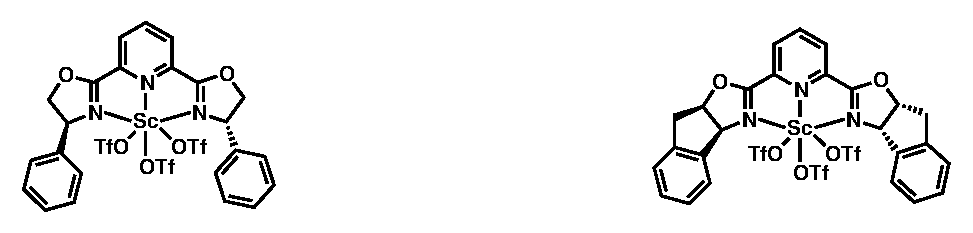
\includegraphics[scale=0.8]{chp_asymmetric/images/evanspybox}
%   \begin{textblock}{5}(-1,-4) \small \textsf{\textit{Evans}
%   \textbf{2001}\crossref{ref:asevans}\textsuperscript{a}}\end{textblock}
%   \begin{textblock}{5}(10,-4) \small \textsf{\textit{Evans}
%   \textbf{2003}\crossref{ref:asevans}\textsuperscript{b}}\end{textblock}  
%   \begin{textblock}{1}(0,-12)
%   \includegraphics[scale=0.35]{chp_asymmetric/images/evanspybox2ortep}\end{textblock}
%   \begin{textblock}{1}(10.5,-13)
%   \includegraphics[scale=0.4]{chp_asymmetric/images/evanspyboxortep}\end{textblock}
%   \caption{Crystal structures of Evan's pybox \ce{Sc(OTf)3} complexes.}
%   \label{fig:evanspybox}
%   \end{figure}  
%  
 We felt confident that by combining scandium (III) salts with the correct chiral ligand, the
 catalyst ligand complex would efficiently direct the stereochemical outcome of the newly forged
 \ce{C-C} bonds. A survey of the Cambridge Structural Database\footnote{{\frenchspacing
 Cambridge Structural Database (WebCSD). http://webcsd.ccdc.cam.ac.uk.proxy.bc.edu (accessed Jan 25, 2013).}} revealed
 four crystal structures containing chiral ligands bound to scandium triflate.
 Among the most well characterized and widely studied are the scandium PyBOX complexes reported by
 the Evans' group (\ref{cmp:asaaaa} and \ref{cmp:asaaab}, \reffigure{xraypage}).\footnote{ (a)
 {\frenchspacing Evans, D.
 A.; Sweeney, Z.
 K.; Rovis, T.; Tedrow, J. S. Highly Enantioselective Syntheses of Homopropargylic Alcohols and Dihydrofurans Catalyzed by a Bis(oxazolinyl)pyridine--Scandium Triflate Complex. \textit{J. Am. Chem. Soc.} \textbf{2001},
 \textit{123}, 12095-12096.} (b) {\frenchspacing Evans, D. A.; Scheidt, K. A.; Fandrick, K. R.; Lam,
 H. W.; Wu, J. Enantioselective Indole Friedel-Crafts Alkylations Catalyzed by
 Bis(oxazolinyl)pyridine--Scandium(III) Triflate Complexes. \textit{J. Am. Chem. Soc.}
 \textbf{2003}, \textit{125}, 10780-10781.} \label{ref:asevans}} Both structures show scandium bound
 with an additional water molecule (omitted from the line drawings for clarity), bringing the
 coordination number to seven.
 Two additional scandium triflate structures, one based on a proline-derived
 \textit{N}-oxide ligand (\ref{cmp:asaaac})\footnote{{\frenchspacing Liu, Y.;
 Shang, D.; Zhou, X.; Liu, X.; Feng, X. Enantioselective Friedel-Crafts Alkylation of Indoles with
 Alkylidene Malonates Catalyzed by \textit{N},\textit{N}-Dioxide-Scandium(III) Complexes:
 Asymmetric Synthesis of $\beta$-Carbolines. \textit{Chem. Eur. J.} \textbf{2009}, \textit{15},
 2055-2058.} \label{ref:asfengstructure}} and one based on a BINOL ligand
 framework\footnote{{\frenchspacing Di Bari, L.; Di Pietro, S.; Pescitelli, G.; Tur, F.; Mansilla,
 J.; Sa\'{a}, J. M. \ce{[Ln(binolam)3].(OTf)3}, a New Class of Propeller-Shaped Lanthanide(III) Salt
 Complexes as Enantioselective Catalysts: Structure, Dynamics and Mechanistic Insight. \textit{Chem.
 Eur. J.} \textbf{2010}, \textit{16}, 14190-14201.}} were reported in 2009 and 2010, respectively. A
 wider search revealed a fifth chiral scandium complex, containing \ce{ScBr3} complexed with a
 bipyridine-based ligand (\ref{cmp:asaaad}).\footnote{{\frenchspacing Ishikawa,
 S.; Hamada, T.; Manabe, K.; Kobayashi, S.
 Catalytic Asymmetric Hydroxymethylation of Silicon Enolates Using an Aqueous Solution of Formaldehyde with a Chiral Scandium Complex. \textit{J. Am. Chem. Soc.}
 \textbf{2004}, \textit{126}, 12236-12237.} \label{ref:askobayashistructure}} 
 
  \begin{figure}[p]
  \centering
  \vspace{1.6in}
  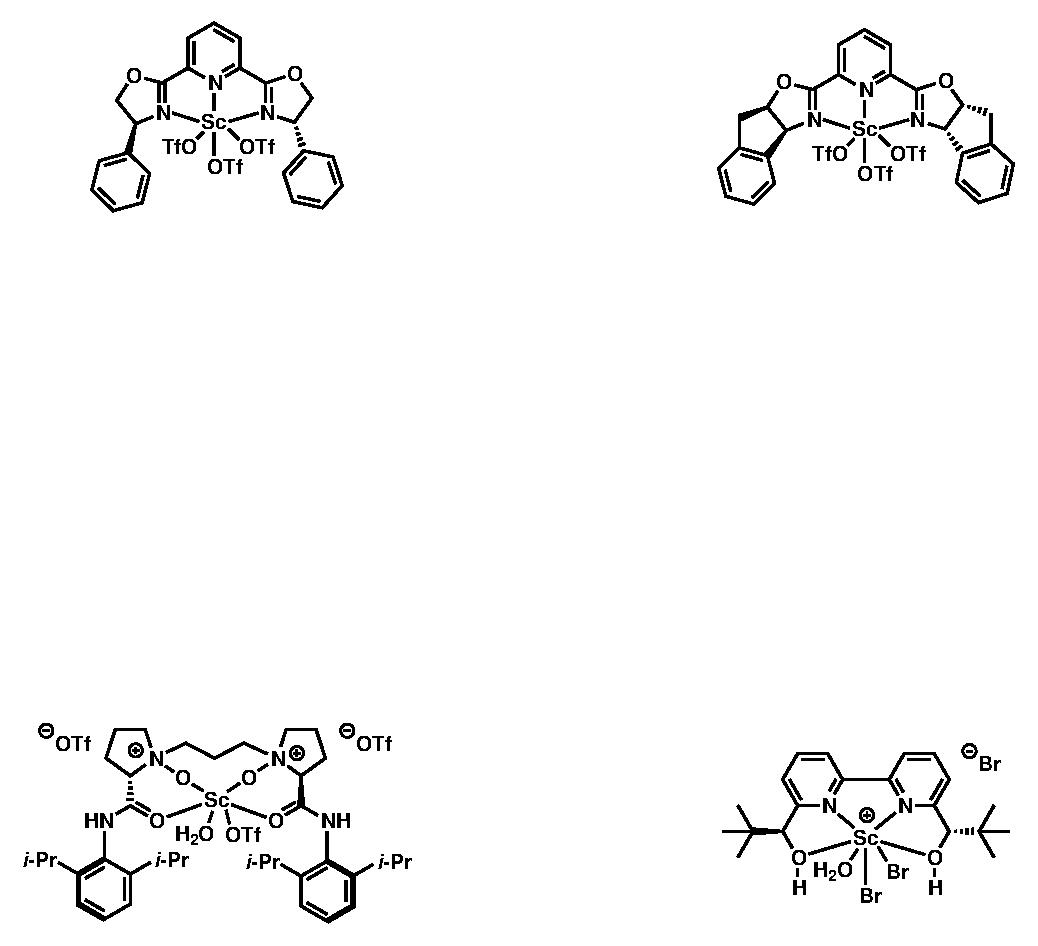
\includegraphics[scale=0.8]{chp_asymmetric/images/xraypage}
  %%%%% references
  \begin{textblock}{5}(2,-12.5) \small \textsf{\textit{Evans}
  \textbf{2001}\crossref{ref:asevans}\textsuperscript{a}}\end{textblock}
  \begin{textblock}{5}(14,-12.5) \small \textsf{\textit{Evans}
  \textbf{2003}\crossref{ref:asevans}\textsuperscript{b}}\end{textblock}
    \begin{textblock}{5}(2.1,0) \small \textsf{\textit{Feng}
   \textbf{2009}\crossref{ref:asfengstructure}}\end{textblock}
   \begin{textblock}{5}(14,0) \small \textsf{\textit{Kobayashi}
   \textbf{2004}\crossref{ref:askobayashistructure}}\end{textblock} 
   %%%% compound numbers
   \begin{textblock}{1}(1.5,-15) \cmp{asaaaa} \end{textblock}
   \begin{textblock}{1}(13.5,-15.5) \cmp{asaaab} \end{textblock}
   \begin{textblock}{1}(0.5, -2.5) \cmp{asaaac} \end{textblock}
   \begin{textblock}{1}(13,-3) \cmp{asaaad} \end{textblock}
   %%%% crystal structures
   \begin{textblock}{1}(0,-24.5)
   \includegraphics[scale=0.35]{chp_asymmetric/images/evanspybox2ortep}\end{textblock}
   \begin{textblock}{1}(10.5,-25.5)
   \includegraphics[scale=0.4]{chp_asymmetric/images/evanspyboxortep}\end{textblock}
   \begin{textblock}{1}(10,-11.5)
   \includegraphics[scale=0.3]{chp_asymmetric/images/kobayashibromideortep}\end{textblock}
    \begin{textblock}{1}(-1,-12.5)
  \includegraphics[scale=0.35]{chp_asymmetric/images/fengoxideortep}\end{textblock}
  \vspace{0.3in}
  \caption{Crystal structures of selected chiral scandium complexes.}
  \label{fig:xraypage}
  \end{figure}
 
 Three of the four
 structures in \reffigure{xraypage} contain a seven
 coordinate pentagonal bipyramidal metal geometry. Scandium (III), because of its filled valence shell
 and lack of \textit{d} electrons, tends to adopt coordination geometries that are based primarily
 on steric constraints rather than traditional orbital overlap based geometries
 observed for the transition metals.\footnote{{\frenchspacing Wu, J. Enantioselective
 Lanthanide-Catalyzed Mukaiyama Aldol, Carbonyl-Ene, Sakurai-Hosomi, and Quinone Diels-Alder Reactions. Ph.D. Dissertation, Harvard University, Cambridge, MA, 2005.} } The
 literature clearly shows precedents for scandium to form well-defined and competent chiral
 catalysts. Chiral scandium complexes have been used to
 catalyze a number of asymmetric \ce{C-C} bond forming reactions.\footnote{For reviews see: (a) {\frenchspacing Kobayashi, S.
 Scandium Triflate in Organic Synthesis. \textit{Eur. J. Org. Chem.} \textbf{1999}, 15-27.} (b)
 {\frenchspacing Mikami, K.; Terada, M.; Matsuzawa, H.
 ``Asymmetric'' Catalysis by Lanthanide Complexes. \textit{Angew. Chem. Int. Ed.} \textbf{2002},
 \textit{41}, 3512-3554.} (c) {\frenchspacing Kobayashi, S.; Sugiura, M.; Kitagawa, H.; Lam, W. W.
 L. Rare-Earth Metal Triflates in Organic Synthesis. \textit{Chem. Rev.} \textbf{2002},
 \textit{102}, 2227-2302.}} 
 


 
%  \begin{figure}[h]
%   \centering
%   \vspace{2.5in}
%   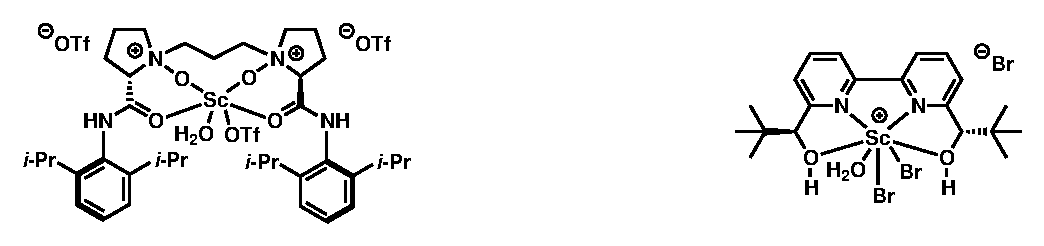
\includegraphics[scale=0.8]{chp_asymmetric/images/fengkobxrays}
%   \begin{textblock}{5}(2.1,0) \small \textsf{\textit{Feng}
%   \textbf{2009}\crossref{ref:asfengstructure}}\end{textblock}
%   \begin{textblock}{5}(14,0) \small \textsf{\textit{Kobayashi}
%   \textbf{2004}\crossref{ref:askobayashistructure}}\end{textblock}  
%   \begin{textblock}{1}(-1,-13)
%   \includegraphics[scale=0.6]{chp_asymmetric/images/fengoxideortep}\end{textblock}
%   \begin{textblock}{1}(10,-11.5)
%   \includegraphics[scale=0.35]{chp_asymmetric/images/kobayashibromideortep}\end{textblock}
%   \vspace{20pt}
%   \caption{Crystal structures of chiral scandium complexes.}
%   \label{fig:fengkobxrays}
%   \end{figure}  
  
  In the sections that follow, an account of how we developed the first catalytic asymmetric
  diazoalkane carbon insertion reactions is presented. The crystallographic data from the literature
  suggests a logical starting point for the development of a new method based on chiral scandium complexes. Ligand constructs
 known to form competent catalysts with Sc(III) salts would be among the first screened for
 asymmetric induction. Before discussing
  experimental details, a brief background on alternative methods for the synthesis of
  $\alpha$-substituted cycloalkanones is given. 
 
 \pagebreak
 \section{Methods for Asymmetric $\alpha$-Functionalization of
 Cycloalkanones}
 
 \subsection{Construction of $\alpha$-Tertiary Centers}
 
 One of the most common methods for \ce{C-C} bond construction involves the
 $\alpha$-functionalization of ketone enolates.
 Some of the first sucessful methods for $\alpha$-functionalized of cycloalkanes in a
 stereocontrolled fashion relied extensively on the pre-formation of chiral imines or hydrazones. In
 1976, Meyers and coworkers reported a highly enantioselective synthesis of 2-alkyl substituted
 cyclohexanones through the formation of a lithio-chelated enamine
 nucleophile (\ref{cmp:asaab}, \refscheme{asmeyers}).\footnote{{\frenchspacing Meyers, A. I.;
 Williams, D.
 R.; Druelinger, M.
 Enantioselective Alkylation of Cyclohexanone via Chiral Lithio-Chelated Enamines. \textit{J. Am.
 Chem. Soc.} \textbf{1976}, \textit{98}, 3032-3033.}} Upon treatment with an alkyl electrophile,
 a stereoselective trap of the electrophile lead to products in up to 97.5:2.5 er
 after careful imine hydrolysis.
 The introduction of a chelating methyl ether moiety rigidified the proposed metalloenamine
 intermediate \ref{cmp:asaab} and led to much higher levels of stereocontrol than previous reports
 with imines that lacked an additional chelating group.\footnote{(a) {\frenchspacing Mea-Jacheet, D.; Horeau, A. Asymmetric Synthesis and Optical purity of 2-Methylcyclohexanone. \textit{Bull. Soc. Chim. Fr.} \textbf{1968}, 4571-4573.} (b) {\frenchspacing Kitamoto, M.; Hiroi, K.; Terashima, S.
 Stereochemical Studies. XXIX. Asymmetric Synthesis of 2-Alkylcyclohexanones via Optically Active
 Lithioenamines. \textit{Chem. Pharm. Bull.} \textbf{1974}, \textit{22}, 459-464.}} 
  \begin{Scheme}[h]
  \centering
  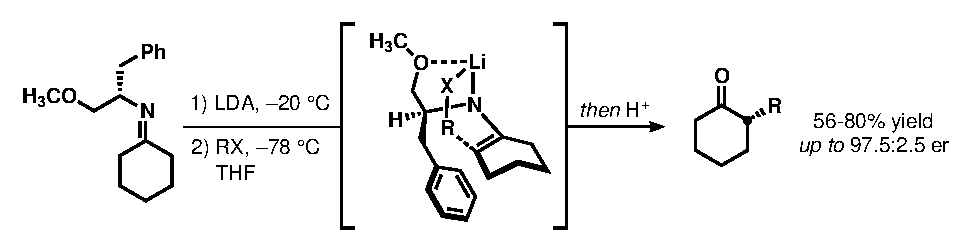
\includegraphics[scale=0.8]{chp_asymmetric/images/meyers}
  \begin{textblock}{1}(7.8,-1) \cmp{asaab} \end{textblock}
  \caption{Meyers auxiliary based approach for $\alpha$-alkylation.}
  \label{sch:asmeyers}
\end{Scheme}   
 
 Around the time of Meyers work, the Enders group introduced the proline derived chiral auxiliary
 (\textit{S})-1-amino-2-methoxymethylpyrrolidine (SAMP, \ref{cmp:asaad}, \refscheme{assamp}), which
 contained a very similar chelating functional group.\footnote{{\frenchspacing Enders, D.; Eichenauer, H.
 Asymmetric Synthesis of $\alpha$-Substituted Ketones by Metalation and Alkylation of Chiral Hydrazones. \textit{Angew.
 Chem. Int. Ed.} \textbf{1976}, \textit{15}, 549-551.}} The SAMP auxiliary and related derivatives
 have been widely utilized for their often very high and predictable levels of stereoinduction and
 for their mild and varied means of cleavage.\footnote{For a recent review see: {\frenchspacing Job, A.; Janeck, C. F.; Bettray, W.;
 Peters, R.; Enders, D. The SAMP-/RAMP-Hydrazone Methodology in Asymmetric Synthesis.
 \textit{Tetrahedron} \textbf{2002}, \textit{58}, 2253-2329.}} In the context of a cycloheptanone
 substrate, the Holmes group sucessfully applied a SAMP hydrazone alkylation strategy to their
 enantioselective synthesis of ($-$)-gloeosporone
 (\ce{->}\ref{cmp:asaac}, \refscheme{assamp}).\footnote{{\frenchspacing Curtis, N.
 R.; Holmes, A. B.; Looney, M. G.; Pearson, N. D.; Slim, G. C. Synthesis of ($-$)-Gloeosporone.
 \textit{Tetrahedron Lett.} \textbf{1991}, \textit{32}, 537-540.}} Cleavage of the auxiliary was
 achieved by treatment with ozone at low temperature, delivering the target cycloheptanone
 \ref{cmp:asaaca} in 97:3 er. 
 \begin{Scheme}[t]
  \centering
  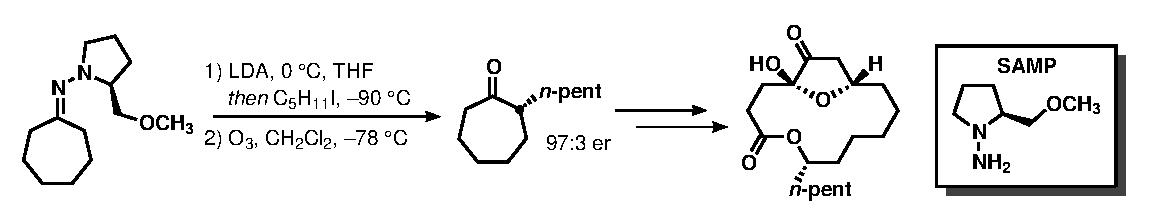
\includegraphics[scale=0.8]{chp_asymmetric/images/samp}
  \begin{textblock}{1}(8.5,-0.5) \cmp{asaaca} \end{textblock}
  \begin{textblock}{1}(15,-1) \cmp{asaac} \end{textblock}
  \begin{textblock}{1}(18,-1) \cmp{asaad} \end{textblock}
  \caption{Application of Ender's SAMP auxiliary in total synthesis.}
  \label{sch:assamp}
\end{Scheme}   
 
More modern strategies have focused on the use of chiral catalysts to control stereochemistry, which
foregoes the need to pre-install a costly chiral auxiliary in the substrate. The formation of an
$\alpha$-tertiary center requires control over either the installation of the $\alpha$-substituent
through an asymmetric alkylation event or control over installation of the $\alpha$-hydrogen. Aside
from stoichiometric auxiliary-based approaches, catalytic methods for enolate alkylation based on
phase transfer catalysts\footnote{{\frenchspacing Dolling, U. H.; Davis, P.; Grabowski, E. J. J.
Efficient Catalytic Asymmetric Alkylations. 1. Enantioselective Synthesis of (+)-Indacrinone
\textit{via} Chiral Phase-Transfer Catalysis. \textit{J. Am. Chem. Soc.} \textbf{1984}, \textit{106}, 446-447.}} and chiral lithium enolates\footnote{{\frenchspacing Imai, M.; Hagihara, A.; Kawasaki, H.; Manabe, K.; Koga, K. Catalytic Asymmetric Benzylation of Achiral Lithium Enolates Using a Chiral Ligand for Lithium in the Presence of an Achiral Ligand. \textit{J. Am. Chem. Soc.}
\textbf{1994}, \textit{116}, 8829-8830.}} have also been demonstrated. Alternative approaches have
examined catalytic methods for the installation of an $\alpha$-hydrogen through an enantioselective
enolate protonation event.\footnote{For a review see:
{\frenchspacing Mohr, J.
T.; Hong, A.
Y.; Stoltz, B.
M.
Enantioselective Protonation. \textit{Nature Chem.} \textbf{2009}, \textit{1}, 359-369.}} Achieving
stereocontrol while delivering a group as small as a proton has been a significant challenge and
the subject of considerable research.
 
In 2005, the Yanagisawa group introduced an asymmetric protonation method utilizing a simple
catalyst system derived from commercially available silver fluoride and (\textit{R})-BINAP.\footnote{{\frenchspacing Yanagisawa, A.; Touge, T.; Arai, T.
Enantioselective Protonation of Silyl Enolates Catalyzed by a
\ce{Binap.AgF} Complex. \textit{Angew. Chem. Int. Ed.} \textbf{2005}, \textit{44}, 1546-1548.}
\label{ref:asyanagisawa}} Starting from a pre-formed silyl enol ether, face selective delivery of
the proton from methanol was proposed to proceed through a silver fluoride BINAP complex that delivered methanol while
concomitantly deprotecting the silyl ether (\ref{cmp:asaae}, \refscheme{asyanagisawaproton}). High
yields and near perfect enantioselectivities were observed across a range of 2-aryl substituted cyclic substrates. The
Yamamoto group also demonstrated a very similar asymmetric protonation reaction with a comparable
substrate scope using a non-commercial chiral phosphoric acid catalyst.\footnote{{\frenchspacing
Cheon, C.
H.; Yamamoto, H.
A Br\o nsted Acid Catalyst for the Enantioselective Protonation Reaction. \textit{J. Am. Chem. Soc.}
 \textbf{2008}, \textit{130}, 9246-9247.}}  
\begin{Scheme}[h]
  \centering
  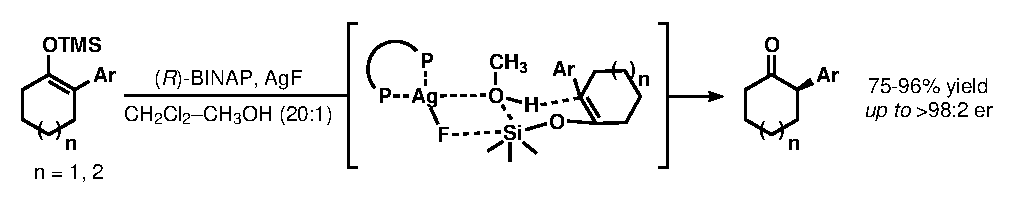
\includegraphics[scale=0.8]{chp_asymmetric/images/yanagisawaproton}
  \begin{textblock}{1}(11,-0.5) \cmp{asaae} \end{textblock}
  \caption{Yanagisawa's asymmetric protonation of silyl enol ethers.}
  \label{sch:asyanagisawaproton}
\end{Scheme}  
 
 
 
 The Stoltz group has also examined enantioselective protonation reactions in the context
 of palladium enolates.\footnote{(a) {\frenchspacing Mohr, J. T.; Nishimata, T.; Behenna, D.
 C.; Stoltz, B.
 M.
 Catalytic Enantioselective Decarboxylative Protonation. \textit{J. Am. Chem. Soc.} \textbf{2006},
 \textit{128}, 11348-11349.} (b) {\frenchspacing Marinescu, S. C.; Nishimata, T.; Mohr, J. T.;
 Stoltz, B. M.
 Homogeneous Pd-Catalyzed Enantioselective Decarboxylative Protonation. \textit{Org. Lett.}
 \textbf{2008}, \textit{10}, 1039-1042.} \label{ref:stoltzprotonation}} When a racemic allyl
 $\beta$-ketoester (\ref{cmp:asaaf}, \refscheme{asstoltzprotonation}) is combined with Pd(0) in the presence of
 PHOX ligand \ref{cmp:asaah}, oxidative addition to the allyl group followed by decarboxylation
 furnishes a chiral palladium enolate intermediate. By adding a superstoichiometric amount of
 Meldrum's acid (\ref{cmp:asaag}, 2.5 equiv), the reaction can be effectively interrupted before
 reductive elimination to deliver $\alpha$-tertiary substituted cycloalkanones in high yields and enantioselectivities. The catalytic cycle is closed by ultimately delivering the allyl fragment to the Meldrum's acid enolate, regenerating the
 Pd(0) catalyst.
  \begin{Scheme}[h]
  \centering
  \includegraphics[scale=0.8]{chp_asymmetric/images/stoltzprotonation}
  \begin{textblock}{1}(1.5,-1.5) \cmp{asaaf} \end{textblock}
  \begin{textblock}{1}(4.9,-1.5) \cmp{asaag} \end{textblock}
  \begin{textblock}{1}(16,-1) \cmp{asaah} \end{textblock}
  \begin{textblock}{1}(8.5,-3.37) \crossrefcmp{asaah} \end{textblock}
  \caption{Stoltz's asymmetric protonation of Pd-enolates.}
  \label{sch:asstoltzprotonation}
\end{Scheme}   
 
 
 Another strategy, not based on enolate alkylation or asymmetric protonation, was developed by the
 Hoveyda group. Enantioselective conjugate addition of alkylzinc reagents to nitroalkenes catalyzed
 by a chiral copper complex, followed by acidic Nef hydrolysis, affords $\alpha$-tertiary
 substituted cycloalkanones (\refscheme{ashoveydaconj}).\footnote{{\frenchspacing Luchaco-Cullis, C.
 A.; Hoveyda, A.
 H.
 Cu-Catalyzed Enantioselective Conjugate Addition of Alkylzincs to Cyclic Nitroalkenes: Catalytic
 Asymmetric Synthesis of Cyclic $\alpha$-Substituted ketones. \textit{J. Am. Chem. Soc.}
 \textbf{2002}, \textit{124}, 8192-8193.}} The hydrolysis, carried out in a subsequent step with
 20\% aqueous sulfuric acid, leads to minimal racemization of the products. Notably, the method
 was amenable to the synthesis of a variety of ring sizes and high levels of enantioselectivity
 were observed from 5 to 12 membered rings.
 
 
 \begin{Scheme}[h]
  \centering \includegraphics[scale=0.8]{chp_asymmetric/images/hoveydaconj}
  \begin{textblock}{1}(13,-1) \cmp{asaai} \end{textblock}
  \begin{textblock}{1}(3.8,-3) \crossrefcmp{asaai} \end{textblock}
  \caption{Hoveyda's conjugate addition to nitroalkenes.}
  \label{sch:ashoveydaconj}
\end{Scheme}   
 
 
 The Shi group introduced a two-step protocol to access optically active
 2-aryl cyclopentanones using an enantioselective epoxidation of
 cyclobutylidene olefins (\refscheme{asshirearrangement}).\footnote{{\frenchspacing Shen, Y.-M.;
 Wang, B.; Shi, Y.
 Enantioselective Synthesis of 2-Aryl Cyclopentanones by Asymmetric Epoxidation and Epoxide Rearrangement. \textit{Angew. Chem.
 Int. Ed.} \textbf{2006}, \textit{45}, 1429-1432.} \label{ref:asshitertiary}} Treatment of
 trisubstituted cyclobutylidene olefins with catalyst \ref{cmp:asaaj} in the presence of Oxone\regtm\  delivered
 the intermediate chiral epoxides in high yields and enantioselectivities. Upon exposure of the
 epoxides to \ce{Et2AlCl}, a facile and highly selective rearrangement to the 2-aryl substituted
 cyclopentanones occurred. Shi also showed that by simply adding lithium iodide during the
 Lewis-acid mediated rearrangement, the opposite enantiomer of the cyclopentanones could be obtained with high
 stereochemical fidelity. This obviates the need to synthesize the opposite enantiomer of catalyst
 \ref{cmp:asaaj}, which can often be challenging if the source of chirality is ultimately derived
 from a chiral pool molecule. This method was extended to the synthesis of $\alpha$-quaternary
 cyclopentanones by starting from tetrasubstituted cyclobutylidene olefins.\footnote{{\frenchspacing Shen, Y.-M.; Wang, B.; Shi, Y. Enantioselective Synthesis of 2-Alkyl-2-Aryl Cyclopentanones by Asymmetric Epoxidation of Tetrasubstituted Cyclobutylidene Olefins and Epoxide Rearrangement. \textit{Tetrahedron Lett.} \textbf{2006}, \textit{47}, 5455-5458.}} 
 \begin{Scheme}[t]
  \centering
  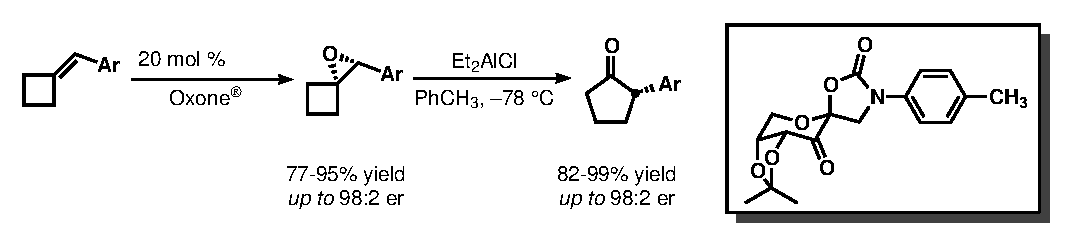
\includegraphics[scale=0.8]{chp_asymmetric/images/shirearrangement}
  \begin{textblock}{1}(16,-1) \cmp{asaaj} \end{textblock}
  \begin{textblock}{1}(4.4,-3.2) \crossrefcmp{asaaj} \end{textblock}
  \caption{Shi's asymmetric epoxidation / rearrangement strategy.}
  \label{sch:asshirearrangement}
\end{Scheme}   
 
  \begin{Scheme}[h]
  \centering
  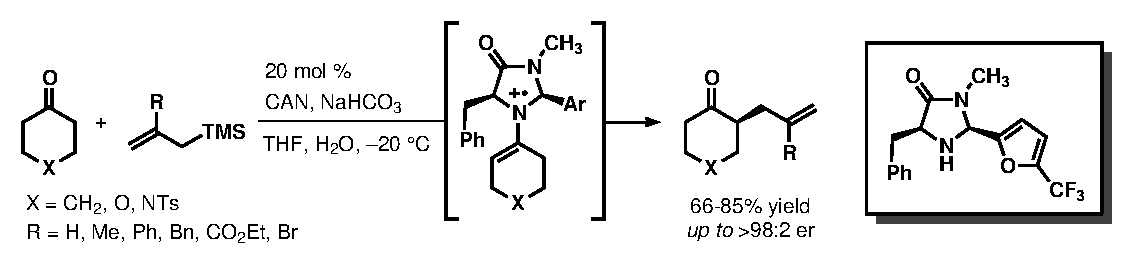
\includegraphics[scale=0.8]{chp_asymmetric/images/macmillansomo}
  \begin{textblock}{1}(9.5,-1) \cmp{asaaja} \end{textblock}
  \begin{textblock}{1}(18.3,-3.2) \cmp{asaajb} \end{textblock}
  \begin{textblock}{1}(6.1,-3.32) \crossrefcmp{asaajb} \end{textblock}
  \caption{Asymmetric allylation with MacMillan's SOMO catalysis.}
  \label{sch:macmillansomo}
\end{Scheme}   
 In 2010 MacMillian reported an intriguing new organocatalytic allylation
 method (\refscheme{macmillansomo}).\footnote{{\frenchspacing Mastracchio, A.; Warkentin, A.
 A.; Walji, A.
 M.; MacMillan, D. W. C. Direct and Enantioselective $\alpha$-Allylation of Ketones \textit{via}
 Singly Occupied Molecular Orbital (SOMO) Catalysis. \textit{Proc. Natl. Acad. Sci. U.S.A.}
 \textbf{2010}, \textit{107}, 20648-20651.} \label{ref:macmillansomo}} Treatment of unfunctionalized
 cycloalkanones with \ref{cmp:asaajb} and CAN facilitates access to a unique three electron
 $\pi$-system (\ref{cmp:asaaja}) through a single electron oxidation event. Face-selective radical
 coupling with substituted allyl trimethylsilanes lead directly to $\alpha$-tertiary substituted
 chiral cycloalkanones with excellent enantioselectivity. 

 
 \subsection{Construction of $\alpha$-Quaternary Centers}
 
 The construction of quaternary centers, especially those possessing all-carbon
 substituents, presents a significant and ongoing challenge for synthetic
 chemists.\footnote{For a reviews on methods for all-carbon quaternary center construction see: (a)
 {\frenchspacing Trost, B. M.; Jiang, C. Catalytic Enantioselective Construction of All-Carbon
 Quaternary Stereocenters. \textit{Synthesis} \textbf{2006}, 369-396.} (b) {\frenchspacing Douglas,
 C.
 J.; Overman, L.
 E.
 Catalytic Asymmetric Synthesis of All-Carbon Quaternary Stereocenters. \textit{Proc. Natl. Acad.
 Sci. U.S.A.} \textbf{2004}, \textit{101}, 5363-5367.}} In their seminal work, Doyle and Jacobsen
 demonstrated a highly enantioselective catalytic asymmetric alkylation of tin enolates to form
 products bearing all-carbon quaternary centers
 (\refscheme{asjacobsentin}).\footnote{{\frenchspacing Doyle, A.
 G.; Jacobsen, E.
 N.
 Enantioselective Alkylations of Tributyltin Enolates Catalyzed by Cr(salen)Cl: Access to Enantiomerically Enriched
 All-Carbon Quaternary Centers. \textit{J. Am. Chem. Soc.} \textbf{2005}, \textit{127}, 62-63.}}
 Tetrasubstituted tin enolates underwent smooth conversion to the $\alpha$-quaternary cycloalkanones
 upon treatment with chromium salen complex \ref{cmp:asaak} and an appropriate alkyl electrophile.
 Cycloalkanones of varying ring sizes were isolated in moderate to high yields with excellent levels of stereocontrol over the newly constructed \ce{C-C} bond. Trisubstituted tin
 enolates that would lead to $\alpha$-tertiary products decomposed under the reaction conditions and
 afforded products in low yields and modest enantioselectivities.
  \begin{Scheme}[h]
  \centering
  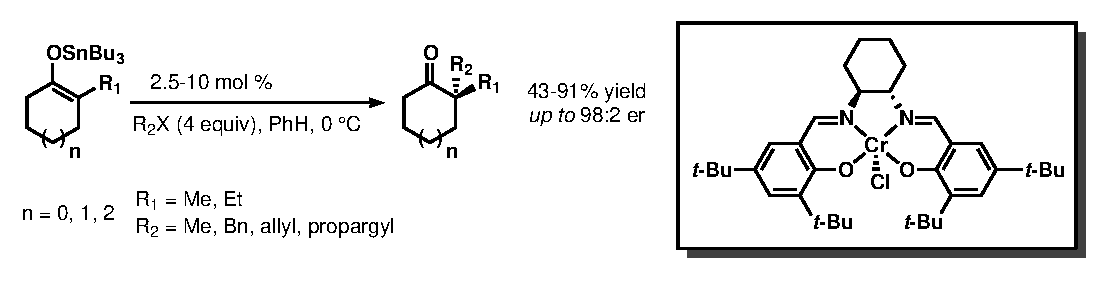
\includegraphics[scale=0.8]{chp_asymmetric/images/jacobsentin}
   \begin{textblock}{1}(12.5,-4) \cmp{asaak} \end{textblock}
  \begin{textblock}{1}(5,-3.35) \crossrefcmp{asaak} \end{textblock}
  \caption{Jacobsen's asymmetric alkylation of tin enolates.}
  \label{sch:asjacobsentin}
\end{Scheme}   
 
The Buchwald\footnote{(a) {\frenchspacing \AA
hman, J.; Wolfe, J.
P.; Troutman, M.
V; Palucki, M.; Buchwald, S. L. Asymmetric Arylation of Ketone Enolates. \textit{J. Am. Chem. Soc.}
 \textbf{1998}, \textit{120}, 1918-1919.} (b) {\frenchspacing Hamada, T.; Chieffi, A.; \AA hman, J.; Buchwald, S. L. An Improved Catalyst for the Asymmetric Arylation of Ketone Enolates. \textit{J. Am. Chem.
 Soc.} \textbf{2002}, \textit{124}, 1261-1268.} \label{ref:asbuchwaldarylation}} and
 Hartwig\footnote{{\frenchspacing Liao, X.; Weng, Z.; Hartwig, J. F. Enantioselective $\alpha$-Arylation of Ketones with Aryl Triflates Catalyzed by Difluorphos Complexes of Palladium
 and Nickel. \textit{J. Am. Chem. Soc.} \textbf{2008}, \textit{130}, 195-200.}} groups introduced similar cross-coupling strategies to access
 all-carbon quaternary centers containing an aromatic substituent. In Buchwald's approach, a two step sequence involving formylation and condensation to prepare an $\alpha$' blocked vinylogous amide
(\ref{cmp:asaal}, \refscheme{asbuchwaldarylation}) was necessary to prevent enolization and coupling
from occuring on the left half of the molecule.
Hartwig focused on indanone and tetralone substrates lacking enolizable $\alpha$' protons
(\refscheme{ashartwigarylation}).
Both methods utilized sodium \textit{tert}-butoxide to generate a sodium enolate that
transmetallated to a chiral Pd(II) or Ni(II) intermediate and ultimately underwent a stereoselective
reductive elimination to forge the new \ce{C-aryl} bond. Buchwald then cleaved the vinylogous amide
protecting group through a dilute acid mediated retro-Claisen condensation. The primary differences
between the two methods were in the choice of chiral ligand and aryl coupling partner. Buchwald
later expanded the substrate scope to include vinyl electrophiles.\footnote{{\frenchspacing Chieffi, A.; Kamikawa, K.; \AA hman, J.; Fox, J. M.; Buchwald, S. L. Catalytic Asymmetric Vinylation of Ketone Enolates. \textit{Org. Lett.}
 \textbf{2001}, \textit{3}, 1897-1900.}}  
   \begin{Scheme}[h]
  \centering
  \includegraphics[scale=0.8]{chp_asymmetric/images/buchwaldarylation}
  \begin{textblock}{1}(2.5,-1.5) \cmp{asaal} \end{textblock}
  \begin{textblock}{1}(17,-0.8) \cmp{asaam} \end{textblock}
  \begin{textblock}{1}(6.1,-3.78) \crossrefcmp{asaam} \end{textblock}
  \caption{Buchwald's asymmetric arylation of $\alpha$'-blocked cycloalkanones.}
  \label{sch:asbuchwaldarylation}
\end{Scheme}   
    \begin{Scheme}[h]
  \centering
  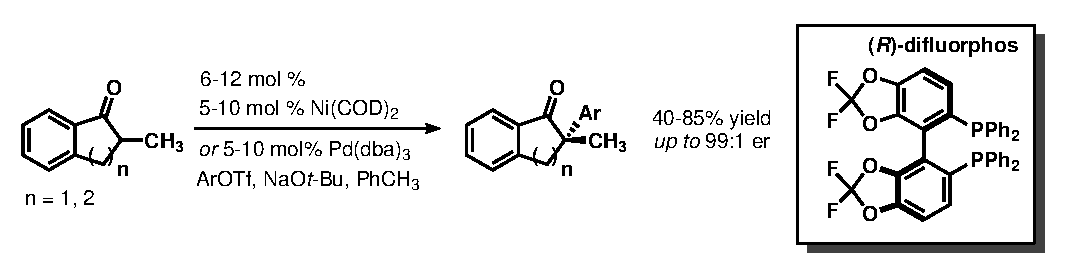
\includegraphics[scale=0.8]{chp_asymmetric/images/hartwigarylation}
  \begin{textblock}{1}(17.5,-0.8) \cmp{asaan} \end{textblock}
  \begin{textblock}{1}(6,-3.35) \crossrefcmp{asaan} \end{textblock}
  \caption{Hartwig's asymmetric arylation of $\alpha$'-blocked cycloalkanones.}
  \label{sch:ashartwigarylation}
\end{Scheme}   
 
 
 The Trost\footnote{{\frenchspacing Trost, B. M.; Schroeder, G. M.
 Palladium-Catalyzed Asymmetric Allylic Alkylation of Ketone Enolates. \textit{J. Am. Chem. Soc.}
 \textbf{2004}, \textit{121}, 6759-6760.}} and Stoltz\footnote{(a) {\frenchspacing Behenna, D.
 C.; Stoltz, B.
 M.
 The Enantioselective Tsuji Allylation. \textit{J. Am. Chem. Soc.} \textbf{2004}, \textit{126}, 15044-15045.} (b)
 {\frenchspacing Mohr, J. T.; Behenna, D. C.; Harned, A. M.; Stoltz, B. M. Deracemization of
 Quaternary Stereocenters by Pd-Catalyzed Enantioconvergent Decarboxylative Allylation of Racemic
 $\beta$-Ketoesters. \textit{Angew. Chem. Int. Ed.} \textbf{2005}, \textit{44}, 6924-6927.}} groups both developed palladium mediated enolate allylation methods that
 generate $\alpha$-keto all-carbon quaternary centers. In Stoltz's work, starting from either the
 $\beta$-keto allyl ester (\ref{cmp:asaao}, \refscheme{stoltzallylation}) or allyl enol carbonate
 (\ref{cmp:asaap}) lead to the same intermediate chiral Pd(II) enolate. Reductive elimination with
 the allyl fragment furnished $\alpha$-quaternary allyl substituted cycloalkanones in high yields
 with excellent levels of enantioselectivity. The mechanistic insight gained through the development of
 this process lead Stoltz to extend this metholodology to allow for the synthesis of
 $\alpha$-tertiary centers through asymmetric protonation as discussed
 previously.\crossref{ref:stoltzprotonation}
  \begin{Scheme}[h]
  \centering
  \includegraphics[scale=0.8]{chp_asymmetric/images/stoltzallylation}
  \begin{textblock}{1}(1.6,-0.9) \cmp{asaao} \end{textblock}
  \begin{textblock}{1}(6.5,-0.9) \cmp{asaap} \end{textblock}
  \caption{Stoltz's asymmetric allylation of Pd-enolates.}
  \label{sch:stoltzallylation}
\end{Scheme}   
 
 With the exception of MacMillan's notable allylation reactions,\crossref{ref:macmillansomo} all of
 the previous examples required a multi-step sequence to install functional group handles that would
 be utilized in the key stereodefining reaction and then ultimately removed to access the target
 cycloalkanone products. We envisioned developing a general strategy to directly access a broad
 range of chiral $\alpha$-substituted cycloalkanones in a single carbon insertion step with aryl--,
 vinyl--, and alkyl-substituted diazoalkanes.
 The versatility and prevalence of the ketone functional group justifies the development of
 methods complementary to those aforementioned.  
 
 \pagebreak
 \section{Discovery of a Catalyst System for Asymmetric $\alpha$-Arylation}
 
 We initially decided to target the enantioselective $\alpha$-arylation of cycloalkanones for two
 primary reasons.
 The Brewer group had recently introduced a mild and operationally simple method for the synthesis of
 aryl-substituted diazoalkanes based on a modified Swern oxidation procedure.\footnote{(a)
 {\frenchspacing Javed, M. I.; Brewer, M. Diazo Preparation \textit{via} Dehydrogenation of
 Hydrazones with Activated DMSO. \textit{Org. Lett.} \textbf{2007}, \textit{9}, 1789-1792.} (b)
 {\frenchspacing Javed, M. I.; Brewer, M. Diphenyldiazomethane. \textit{Org. Synth.} \textbf{2008},
 \textit{85}, 189-195.} \label{ref:asbrewer}}  A simple protocol for preparing the requisite
 diazoalkanes, coupled with the relative stability of aryl-substituted
 diazoalkanes,\footnote{For the relative reactivity of substituted diazoalkanes see \reffigure{nucleophilicity} on page
 \pageref{fig:nucleophilicity}.} made $\alpha$-arylation an ideal proving ground for the first asymmetric insertion
 reactions.

In advance of looking at any catalytic asymmetric reactions, we wanted to run a control experiment
to determine if the products of our reaction would retain their stereochemical information in the
presence of scandium triflate. The Shi group reported earlier that $\alpha$-aryl cyclopentanones
readily racemize on silica gel, presumably through a rather facile enolization
pathway.\crossref{ref:asshitertiary} We began by preparing an optically active sample of
(\textit{R})-2-phenylcycloheptanone according to a three step sequence using the asymmetric
protonation chemistry developed by Yanagisawa
(\refscheme{asracemizationone}).\crossref{ref:asyanagisawa}
  \begin{Scheme}[h]
  \centering
  \includegraphics[scale=0.8]{chp_asymmetric/images/racemizationone}
  \begin{textblock}{1}(0.35,-0.7) \cmp{ascyclohexanone} \end{textblock}
  \begin{textblock}{1}(3.3,-3.3) \cmp{diazoaa} \end{textblock}
  \begin{textblock}{1}(5.8,-0.7) \cmp{xaaa} \end{textblock}
  \begin{textblock}{1}(11.6,-0.7) \cmp{asaaq} \end{textblock}
  \begin{textblock}{1}(18,-0.7) \cmp{asaar} \end{textblock}
  \caption{Preparation of optically active 2-phenylcycloheptanone.}
  \label{sch:asracemizationone}
\end{Scheme}   
Scandium-catalyzed homologation of cyclohexanone with phenyldiazomethane (\ref{cmp:diazoaa})
afforded racemic 2-phenylcycloheptanone (\ref{cmp:xaaa}) in a 65\% distilled yield. Dropwise
addition of 0.95 equivalents of LDA to \ref{cmp:xaaa} followed by trapping with TMSCl selectively
delivered the thermodynamic enol silane \ref{cmp:asaaq} in 85\% yield.
Asymmetric protonation according to the reported conditions provided access
(\textit{R})-2-phenylcycloheptanone (\ref{cmp:asaar}) in 83\% yield and 95:5 er in our
hands.\footnote{The Yanagisawa group reported a 95\% yield and 98.5:1.5 er for the preparation of 
\ref{cmp:asaar}.
See reference \ref{ref:asyanagisawa} for details.} Exposure of \ref{cmp:asaar} to phenyldiazomethane,
\ce{Sc(OTf)3}, or the combination of the two (toluene, 0 \degc, 6 h) resulted in no loss of enantiopurity (95:5 er by chiral SFC analysis). This promising initial result indicated that chiral homologation products should be configurationally
stable under conditions of scandium catalysis. \refscheme{asracemizationone} also
underscores the benefits of eliminating the three step sequence that must precede asymmetric protonation, as products like \ref{cmp:asaar} could
be accessible in a single asymmetric homologation step.


We also wanted to run a simple mechanistic control to determine if the scandium-catalyzed reactions
proceeded through a pathway involving an epoxide intermediate. House had previously shown that
epoxides formed in Lewis acid mediated ring expansion reactions readily underwent rearrangement
to the corresponding aldehydes.\footnote{{\frenchspacing House, H. O.; Grubbs, E. J.; Gannon, W. F.
The Reaction of Ketones with Diazomethane. \textit{J. Am. Chem. Soc.} \textbf{1960}, \textit{82},
4099-4106.}} We had never detected any epoxide or aldehyde byproducts in any scandium catalyzed ring expansion reactions (by $^1$H NMR), but regardless, we carried out the experiment shown in \refscheme{asepoxideexperiment}. Epoxide \ref{cmp:asaara} was obtained
through standard chemistry in an 87\% yield over two steps from cyclohexanone. Subjecting
epoxide \ref{cmp:asaara} to 10 mol \% \ce{Sc(OTf)3} at $-78$ \degc\  for 5 days resulted in $<$2\%
conversion, clearly indicating that it was improbable the scandium catalyzed homologation reactions
involved an epoxide intermediate. The most plausible mechanism was that
previously discussed in the literature, a concerted collapse of a diazonium
betaine to directly deliver the observed ring expanded products
(\refscheme{mechanism}, page \pageref{sch:mechanism}).\crossref{ref:asgutscherev}

 \begin{Scheme}[h]
  \centering
  \includegraphics[scale=0.8]{chp_asymmetric/images/epoxideexperiment}
  \begin{textblock}{1}(3.4,-0.2) \crossrefcmp{ascyclohexanone} \end{textblock}
   \begin{textblock}{1}(9.4,-0.2) \cmp{asaara} \end{textblock}
   \begin{textblock}{1}(14.8,-0.2) \crossrefcmp{xaaa} \end{textblock}
%   \begin{textblock}{1}(11.6,-0.7) \cmp{asaaq} \end{textblock}
%   \begin{textblock}{1}(18,-0.7) \cmp{asaar} \end{textblock}
  \caption{Mechanistic probe of plausible epoxide rearrangement pathway.}
  \label{sch:asepoxideexperiment}
\end{Scheme}   

\subsection{Optimized Conditions for Consistent Reactivity}

\begin{wrapfigure}{r}{2.8in}
  \centering
  \vspace{-40pt}
  \includegraphics[scale=0.3]{chp_asymmetric/images/scandiumhydratedortep}
  %\begin{textblock}{5}(-1,-4) \small \textsf{test}\end{textblock}
  \caption{Crystal structure of \ce{Sc(H2O)9(OTf)3}.}
  \vspace{-25pt}
  \label{fig:asscandiumhydrated}
  \end{wrapfigure}
The newly discovered scandium catalyzed homologation reactions often gave variable and
unpredictable results that appeared to depend on the source of \ce{Sc(OTf)3} and batch of
diazoalkane solution.
In order to obtain meaningful results when optimizing conditions for asymmetric reactions, the reaction
variability would first need to be understood and mitigated. At the time this project began,
no special protocols were in place to purify any of the reaction components. The \ce{Sc(OTf)3} was
often used as received and the aryl-diazoalkanes were prepared by directly following the
reported Brewer procedure.\crossref{ref:asbrewer} In order to mimimize reaction variability, efforts
were undertaken to rigorously purify and dry \textit{all} reaction components: solvents,
\ce{Sc(OTf)3}, ketones, diazoalkanes, and ligands.

Scandium triflate is a deliquescent solid that rapidly absorbs significant quantities of atmospheric
moisture. Crystallographic data from the literature has shown \ce{Sc(OTf)3} to bind up to nine water
molecules (\reffigure{asscandiumhydrated}).\footnote{{\frenchspacing Abbasi, A.; Lindqvist-Reis, P.;
Eriksson, L.; Sandstr\"{o}m, D.; Lidin, S.; Persson, I.; Sandstr\"{o}m, M. Highly Hydrated Cations:
Deficiency, Mobility, and Coordination of Water in Crystalline Nonahydrated Scandium(III),
Yttrium(III), and Lanthanoid(III) Trifluoromethanesulfonates. \textit{Chem. Eur. J.} \textbf{2005},
\textit{11}, 4065-4077.}} Although \ce{Sc(OTf)3} is known to retain catalytic activity even in
aqueous media,\footnote{{\frenchspacing Kobayashi, S.; Hachiya, I. Lanthanide Triflates as
Water-Tolerant Lewis Acids. Activation of Commercial Formaldehyde Solution and Use in the Aldol
Reaction of Silyl Enol Ethers with Aldehydes in Aqueous Media. \textit{J. Org. Chem.} \textbf{1994},
\textit{59}, 3590-3596.}} we had anecdotal evidence that suggested drier conditions lead to higher
reaction efficiencies for diazoalkane insertion reactions.\footnote{Reaction rates can be
approximated visually by the evolution of nitrogen gas and the loss of the characteristic
diazoalkane color.} When Kobayashi first introduced \ce{Sc(OTf)3} in
1993, he reported drying the salt at 200 \degc\ under high vacuum before use.\footnote{{\frenchspacing Kobayashi, S.; Hachiya, I.; Araki, M.; Ishitani, H.
Scandium Trifluoromethanesulfonate (\ce{Sc(OTf)3}). A Novel Reusable Catalyst in the Diels-Alder
Reaction. \textit{Tetrahedron Lett.} \textbf{1993}, \textit{34}, 3755-3758.}} We took this drying
method one step further and dried commercial \ce{Sc(OTf)3} under high vacuum at 200 \degc\  with
inline \ce{P2O5} for 24 hours before taking the salt into an inert atmosphere glove box using
rigorous Schlenk techniques.

Diazoalkane solutions were originally prepared according to the general procedure reported by Brewer.\crossref{ref:asbrewer} In a typical experimental procedure, a
solution of the hydrazone and triethylamine were added dropwise to a cold solution of chlorodimethylsulfonium chloride, formed \textit{in situ} from oxalyl chloride and DMSO (\refscheme{asbrewerswern}).
After stirring for an hour at $-$78 \degc, the reaction mixture was filtered to remove insoluble
triethylammonium chloride and carefully concentrated to remove THF. The neat diazoalkane was then
dissolved in toluene and stored at $-78$ \degc. Following this procedure gave fairly pure
diazoalkane solutions, but we wanted to be sure to remove all traces of Lewis basic impurities. We modified the procedure to include an aqueous workup which
removed any residual triethylamine and DMSO. The oxidation was run for one hour
in a 9:1 \ce{Et2O}:\ce{CH2Cl2} solvent mixture and immediately poured into a separatory funnel
containing an ice cold 50\% solution of aqueous \ce{NH4Cl}. The \ce{NH4Cl} layer was drained and the
organics were washed with \ce{H2O} and saturated \ce{NaHCO3} before drying over solid \ce{K2CO3}. Filtration,
concentration, and finally dissolution in toluene afforded exceptionally pure diazoalkane solutions. 
\begin{Scheme}[h]
  \centering
  \includegraphics[scale=0.8]{chp_asymmetric/images/brewerswern}
  \begin{textblock}{1}(16,-0.7) \crossrefcmp{diazoaa} \end{textblock}
  \caption{Original preparation of aryl-substituted diazoalkanes by Brewer.}
  \label{sch:asbrewerswern}
\end{Scheme}  

Unfortunately, by performing an aqueous workup on the diazoalkanes, we inadvertently introduced an
additional problem. Occasionally we would observe the formation of a white precipitate in some of
the diazoalkane solutions after prolonged storage at $-78$ \degc. After numerous unsuccessful
attempts to isolate and characterize the white precipitate, we realized that it was residual water
from inefficient drying of diazoalkane solution after workup. Although \ce{K2CO3} was not the most
efficient dessicant, the highest yields of diazoalkane were obtained with solutions dried over
\ce{K2CO3}. The residual water was ultimately best removed by carefully gravity filtering the
diazoalkane solution at $-$78 \degc\ in a cold-jacketed dropping funnel, then storing the clear
solution over 3\AA\ molecular sieves.

With rigorously dried \ce{Sc(OTf)3}, pure and dry diazoalkane solutions, distilled ketones, and
solvents passed through an alumina column and stored over 3\AA\ molecular
sieves,\footnote{{\frenchspacing Williams, D.
B.
G.; Lawton, M.
Drying of Organic Solvents: Quantitative Evaluation of the Efficiency of Several Desiccants.
\textit{J. Org. Chem.} \textbf{2010}, \textit{75}, 8351-8354.}} dramatic increases in reaction
efficiency were observed.\footnote{{\frenchspacing Rendina, V. L.; Kaplan, H. Z.; Kingsbury, J. S.
Highly Efficient and Enantioselective $\alpha$-Arylation of Cycloalkanones by Scandium-Catalyzed
Diazoalkane-Carbonyl Homologation. \textit{Synthesis} \textbf{2012}, \textit{44}, 686-693.}
\label{ref:asrendinapsp}} More importantly though, reactions worked in a predictable and
reproducible manner.
When we had prepared racemic 2-phenylcycloheptanone (\ref{cmp:xaaa}) previously,
the reaction was run with 10 mol \% \ce{Sc(OTf)3} and 1.1 equivalents of phenyldiazomethane
(\ref{cmp:diazoaa}) for 16 hours (\refscheme{asracemizationone},
page \pageref{sch:asracemizationone}).
After workup and attempted purification by silica gel chromatography, the desired product was obtained in a quantitative yield but was contaminated with overhomologation byproducts.\footnote{Not isolated, but double insertion was detected by low resolution mass spectrometry. \ce{C20H23O} [M+H]$^+$: 279.1749.} Careful K\"{u}gelrohr distillation delivered analytically pure material in a modest 65\% yield. Under the new drier conditions, running the reaction for 15 minutes with 0.5 mol \% \ce{Sc(OTf)3}, 1.0
equivalents of phenyldiazomethane, and 1.2 equivalents of cyclohexanone, a 92\% isolated yield was
obtained after silica gel chromatography. By modifying the stoichiometry, no further purification
away from overhomologation byproducts was necessary. The reaction rates were so high, an 18 gauge
exit needle was needed to relieve excess pressure generated by the copious amounts of nitrogen gas evolved.
\begin{Scheme}[h]
  \centering
  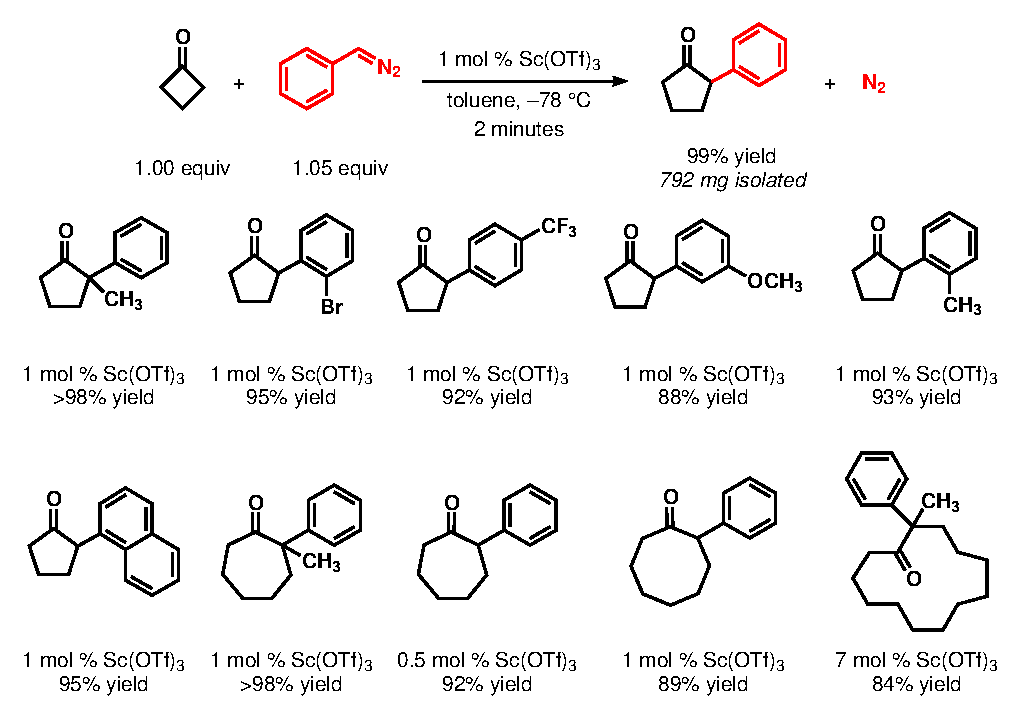
\includegraphics[scale=0.8]{chp_asymmetric/images/rendinapspsubstrates}
  \begin{textblock}{1}(13.5,-10.3) \cmp{xaac} \end{textblock}
  \begin{textblock}{1}(6.5,-10.2) \crossrefcmp{diazoaa} \end{textblock}
  %row 1
  \begin{textblock}{1}(2,-6.6) \cmp{xaab} \end{textblock}
  \begin{textblock}{1}(5.5,-6.6) \cmp{xaad} \end{textblock}
  \begin{textblock}{1}(9,-6.6) \cmp{xaae} \end{textblock}
  \begin{textblock}{1}(12.8,-6.6) \cmp{xaaf} \end{textblock}
  \begin{textblock}{1}(16.5,-6.6) \cmp{xaag} \end{textblock}
  % row 2
\begin{textblock}{1}(2,-1.5) \cmp{xaah} \end{textblock}
\begin{textblock}{1}(5.5,-1.5) \cmp{xaai} \end{textblock}
\begin{textblock}{1}(9,-1.5) \crossrefcmp{xaaa} \end{textblock}
\begin{textblock}{1}(12.8,-1.5) \cmp{xaaj} \end{textblock}
\begin{textblock}{1}(18.2,-3.3) \cmp{xaak} \end{textblock}
  \caption{Highly efficient insertion reactions with aryl-diazoalkanes.}
  \label{sch:asrendinapspsubstrates}
\end{Scheme}  

The newly optimized conditions were successfully applied to a number of ring expansion reactions
with aryl-substituted diazoalkanes (\refscheme{asrendinapspsubstrates}).\crossref{ref:asrendinapsp}
Good scope with regard to the diazoalkane and ketone ring size were demonstrated. Reactions
catalyzed by low loadings of \ce{Sc(OTf)3} (0.5--7 mol \%) were complete in $<$1 hour and gave high
yields in all cases tested. In addition to being reliable and efficient, the reactions could be
scaled to afford gram quantities of homologation products (\ce{->}\ref{cmp:xaac}). With reliable
protocols in place and an understanding that water was the culprit of previous reproducibility
issues, we were prepared to examine asymmetric insertion reactions. 

\subsection{Early Results with Bis(oxazoline) Ligands}

We began by evaluating the PyBOX\crossref{ref:asevans} and bipyridine
diol\crossref{ref:askobayashistructure} ligand frameworks previously reported to form competent
chiral scandium complexes (\refscheme{asinitialligandscreen}). In an inert atmosphere glove box,
\ce{Sc(OTf)3} was stirred in toluene with a slight excess of the ligand for 1.5 hours to pre-form
the ligand-metal complex. During complexation, 25 mol \% THF was added as a cosolvent to help
solubilize the scandium salt. The catalyst mixture was removed from the glove box, connected to a nitrogen manifold, and stirred with cyclohexanone for 15 minutes. After cooling to $-$78 \degc,
phenyldiazomethane (\ref{cmp:diazoaa}) was added in a single portion and the reactions were stirred
until no further evolution of nitrogen gas was observed. An aliquot of the reaction mixture was purified by
preparative thin-layer chromatography and analyzed for optical purity by chiral SFC analysis in
comparison with authentic racemic material. Commercially available PyBOX ligand \ref{cmp:asaas}
delivered \ref{cmp:xaan} in a measurable 56:44 er. The bipyridine diol ligand \ref{cmp:asaat} afforded racemic product. We also tested a
commercially available Salen\footnote{{\frenchspacing Larrow, J. F.; Jacobsen, E. N. Asymmetric
Processes Catalyzed by Chiral (Salen)Metal Complexes. \textit{Topics Organomet. Chem.} \textbf{2004}, \textit{6},
123-152.}} ligand which produced nearly racemic product. Ligands \ref{cmp:asaat} and \ref{cmp:asaau}
were likely not stable under the reaction conditions, as diazoalkanes are known to undergo \ce{O-H}
insertion reactions.\footnote{See the discussion in Chapter \ref{chp:diazobkg} for examples.}
Etherification of the two \ce{O-H} groups would decrease the binding affinity of the ligand and
metal, leading to background reaction by uncomplexed scandium.
\begin{Scheme}[h]
  \centering
  \begin{textblock}{1}(3.1,2.2) \crossrefcmp{ascyclohexanone} \end{textblock}
  \begin{textblock}{1}(6.2,2.2) \crossrefcmp{diazoaa} \end{textblock}
  \begin{textblock}{1}(13.3,2.6) \cmp{xaan} \end{textblock}
  \begin{textblock}{1}(2.6,5.3) \cmp{asaas} \end{textblock}
  \begin{textblock}{1}(8.2,5.3) \cmp{asaat} \end{textblock}
  \begin{textblock}{1}(17,3.2) \cmp{asaau} \end{textblock}
  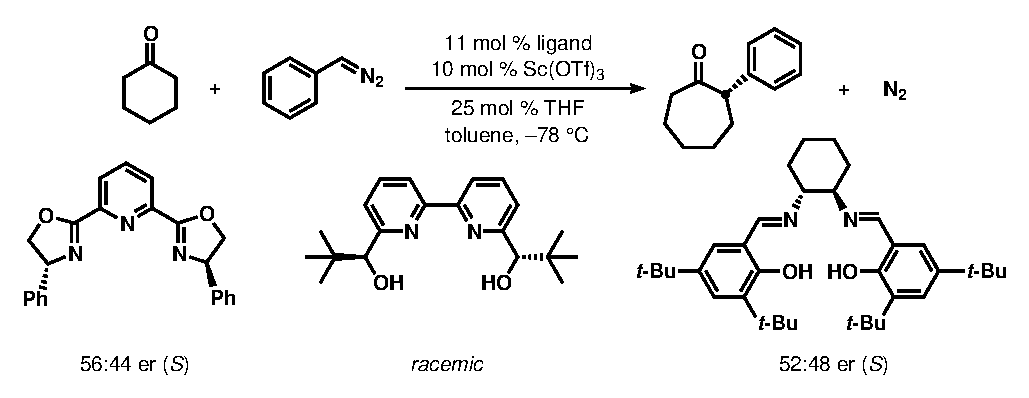
\includegraphics[scale=0.8]{chp_asymmetric/images/initialligandscreen}
  \caption{Initial ligand screening.}
  \label{sch:asinitialligandscreen}
\end{Scheme}  



Previous experiments had shown that Lewis basic impurities could dramatically affect reaction
efficiency. Reactions run with PyBOX ligand \ref{cmp:asaas} visually progressed more slowly than
those without the ligand present. We believed that by excising the bridging pyridine ring, we
could decrease the Lewis basicity of the ligand while simultaneously bringing the ligand blocking
groups closer to the metal center. The well known bis(oxazoline) ligand class retains the blocking
group structure of the PyBOX ligands, but contains a methylene bridge between the two oxazoline
units. While scandium PyBOX crystal structures have been reported, there are no examples of scandium
bis(oxazoline) structures. In contrast, a preponderance of bis(oxazoline) copper
complexes have been reported.\footnote{Nineteen Cu(II) bis(oxazoline) crystal
structures were discussed by Desimoni in a 2006 review. {\frenchspacing Desimoni, G.; Faita, G.;
J\o rgensen, K.
A.
C$_2$-Symmetric Chiral Bis(oxazoline) Ligands in Asymmetric Catalysis. \textit{Chem. Rev.}
\textbf{2006}, \textit{106}, 3561-3651.} \label{ref:asboxreview}} \reffigure{ascoppercomplexes}
shows a direct comparison between copper PyBOX\footnote{{\frenchspacing Evans, D. A.; Kozlowski, M. C.; Murry, J. A.; Burgey,
C. S.; Campos, K. R.; Connell, B. T.; Staples, R. J. C$_2$-Symmetric Copper (II) Complexes as Chiral
Lewis Acids. Scope and Mechanism of Catalytic Enantioselective Aldol Additions of Enolsilanes to
(Benzyloxy)acetaldehyde. \textit{J. Am. Chem. Soc.} \textbf{1999}, \textit{121}, 669-685.}} and
copper BOX\footnote{{\frenchspacing Evans, D. A.; Johnson, J. S.; Burgey, C. S.; Campos,
K. R. Reversal in Enantioselectivity of \textit{tert}-Butyl Versus Phenyl-Substituted Bis(oxazoline)
Copper(II) Catalyzed Hetero Diels-Alder and Ene Reactions. Crystallographic and Mechanistic Studies.
\textit{Tetrahedron Lett.} \textbf{1999}, \textit{40}, 2879-2882.}} hexafluoroantimonate salts
containing the same valine-derived oxazoline units. The BOX complex (right,
\ref{cmp:asaaw}) shows a smaller through space N$_{ox}$\ce{-}N$_{ox}$ distance (1.13 \AA\  shorter)
and a significantly compressed N$_{ox}$\ce{-}Cu\ce{-}N$_{ox}$ internal angle relative to the
corresponding PyBOX complex (left, \ref{cmp:asaav}).
\begin{figure}[t]
\vspace{1.65in}
  \centering
     \begin{textblock}{1}(0.7,1.2) \cmp{asaav} \end{textblock}
   \begin{textblock}{1}(11.7,1.2) \cmp{asaaw} \end{textblock}
  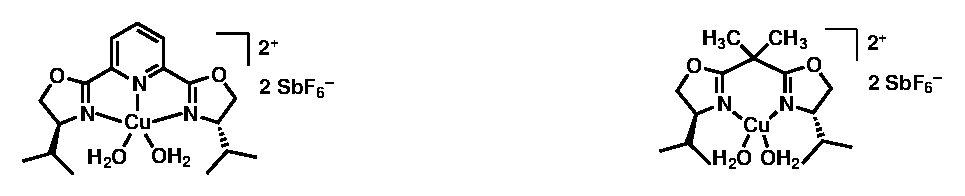
\includegraphics[scale=0.8]{chp_asymmetric/images/evanscopper}
  \begin{textblock}{5}(2,0.5) \small \textsf{N$_{ox}$\ce{-}N$_{ox}$ distance 3.95
  \AA \\ $\angle$ N$_{ox}$\ce{-}Cu\ce{-}N$_{ox}$ 158.4$^\circ$}\end{textblock}
  \begin{textblock}{5}(12.5,0.5) \small \textsf{N$_{ox}$\ce{-}N$_{ox}$ distance 2.82
  \AA \\ $\angle$ N$_{ox}$\ce{-}Cu\ce{-}N$_{ox}$ 91.6$^\circ$}\end{textblock} 
  \begin{textblock}{1}(-1.5,-9)
  \includegraphics[scale=0.3]{chp_asymmetric/images/copperpyboxortep}\end{textblock}
  \begin{textblock}{1}(10,-9)
  \includegraphics[scale=0.3]{chp_asymmetric/images/copperboxortep}\end{textblock}
  \vspace{0.6in}
  \caption{Comparison of copper PyBOX and BOX complexes. Counterions omitted for clarity.}
  \label{fig:ascoppercomplexes}
\end{figure}  


We quickly tested several readily available BOX ligands, hoping the different steric
and electronic properties would translate into increased levels of stereoinduction
(\refscheme{asfirstboxscreen}).
We were pleased to see that ligand \ref{cmp:boxasab} provided much higher levels of selectivity. Different blocking
groups (\ref{cmp:boxasaa}, \ref{cmp:boxasac}) and bis(oxazoline) \ref{cmp:boxasad} resulted in
lower selectivity. Excited by this promising lead, we initiated a broader screen of BOX ligands
(\refscheme{asbigboxscreen}). The bis(oxazoline) framework contains three diversity sites for
C$_2$-symmetric ligands, making it a highly tunable and privileged ligand
class.\crossref{ref:asboxreview} We wanted to simultaneously optimize with regard to both backbone substitution and the amino alcohol derived blocking groups.\footnote{For a lead reference on the
benefits of multi-factor optimization see: {\frenchspacing Lendrem, D.; Owen, M.; Godbert,
S. DOE (Design of Experiments) in Development Chemistry: Potential Obstacles. \textit{Org. Process
Res. Dev.} \textbf{2001}, \textit{5}, 324-327.}}
 \begin{Scheme}[t]
  \centering
   \begin{textblock}{1}(3.1,2.3) \crossrefcmp{ascyclohexanone} \end{textblock}
   \begin{textblock}{1}(6.2,2.3) \crossrefcmp{diazoaa} \end{textblock}
   \begin{textblock}{1}(14,2) \crossrefcmp{xaan} \end{textblock}
   \begin{textblock}{1}(1.6,5.3) \cmp{boxasaa} \end{textblock}
    \begin{textblock}{1}(6.4,5.3) \cmp{boxasab} \end{textblock}
     \begin{textblock}{1}(12,5.3) \cmp{boxasac} \end{textblock}
      \begin{textblock}{1}(17,5.3) \cmp{boxasad} \end{textblock}
  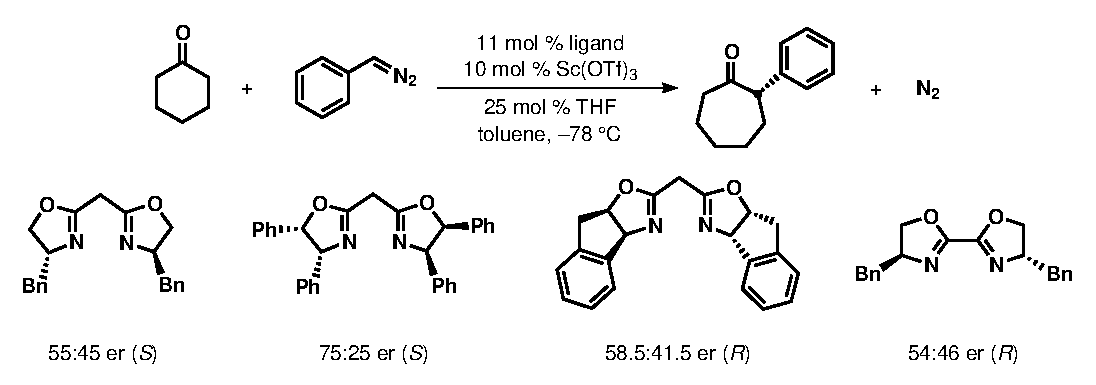
\includegraphics[scale=0.8]{chp_asymmetric/images/firstboxscreen}
  \caption{Screen of commercially available bis(oxazoline) ligands.}
  \label{sch:asfirstboxscreen}
\end{Scheme}

Examination of the results in \refscheme{asbigboxscreen} showed that backbone substitution was
integral to obtaining high levels of induction. Ligands lacking geminal substitution on the bridging
methylene are known to tautomerize, which could adversely impact the ligand-metal
binding. We prepared a series of ligands containing cyclic backbone
substitution to probe the effect of bite angle on enantioselectivity. Davies and coworkers had
prepared a similar series of BOX ligands and observed a strong dependence of enantioselectivity on ligand bite
angle in copper catalyzed Diels-Alder reactions.\footnote{(a) {\frenchspacing Davies, I. W. I. W.;
Gerena, L.; Castonguay, L.; Senanayake, C.
H.; Larsen, R. D.; Verhoevena, T. R.; Reidera, P. J.; Verhoeven, T. R.; Reider, P. J. The Influence
of Ligand Bite Angle on the Enantioselectivity of Copper(II)-Catalysed Diels-Alder Reactions.
\textit{Chem. Commun.} \textbf{1996}, 1753-1754.} (b) {\frenchspacing Davies, I. W.; Deeth, R. J.;
Larsen, R. D.; Reider, P. J. A CLFSE/MM Study on the Role of Ligand Bite-Angle in Cu(II)-Catalyzed
Diels-Alder Reactions. \textit{Tetrahedron Lett.} \textbf{1999}, \textit{40}, 1233-1236.}\label{ref:asdaviesdielsalder}} \begin{Scheme}[p]
  \centering
%% header row
  \begin{textblock}{1}(3,2.3) \crossrefcmp{ascyclohexanone} \end{textblock}
  \begin{textblock}{1}(6.2,2.3) \crossrefcmp{diazoaa} \end{textblock}
  \begin{textblock}{1}(13.3,2.6) \crossrefcmp{xaan} \end{textblock}
%% row 1
   \begin{textblock}{1}(7.4,5.9) \crossrefcmp{boxasaa} \end{textblock}
    \begin{textblock}{1}(11.8,5.9) \crossrefcmp{boxasab} \end{textblock}
     \begin{textblock}{1}(16.5,5.9) \crossrefcmp{boxasac} \end{textblock}
 %% row 2
   \begin{textblock}{1}(2,11) \cmp{ligandac} \end{textblock}
    \begin{textblock}{1}(7.2,11) \cmp{ligandad} \end{textblock}
     \begin{textblock}{1}(12,11) \cmp{ligandae} \end{textblock}
     \begin{textblock}{1}(16.8,11) \cmp{ligandaf} \end{textblock}
 %% row 3
    \begin{textblock}{1}(1.8,15.8) \cmp{boxasae} \end{textblock}
    \begin{textblock}{1}(7,15.8) \cmp{boxasaf} \end{textblock}
     \begin{textblock}{1}(12,15.8) \cmp{ligandal} \end{textblock}
     \begin{textblock}{1}(16.8,15.8) \cmp{boxasag} \end{textblock}
%% row 4
    \begin{textblock}{1}(4.2,20) \cmp{boxasah} \end{textblock}
    \begin{textblock}{1}(9.35,20) \cmp{boxasai} \end{textblock} %% dibenzyl gemdimethyl
     \begin{textblock}{1}(14.65,20) \cmp{ligandaa} \end{textblock} %% indabox
  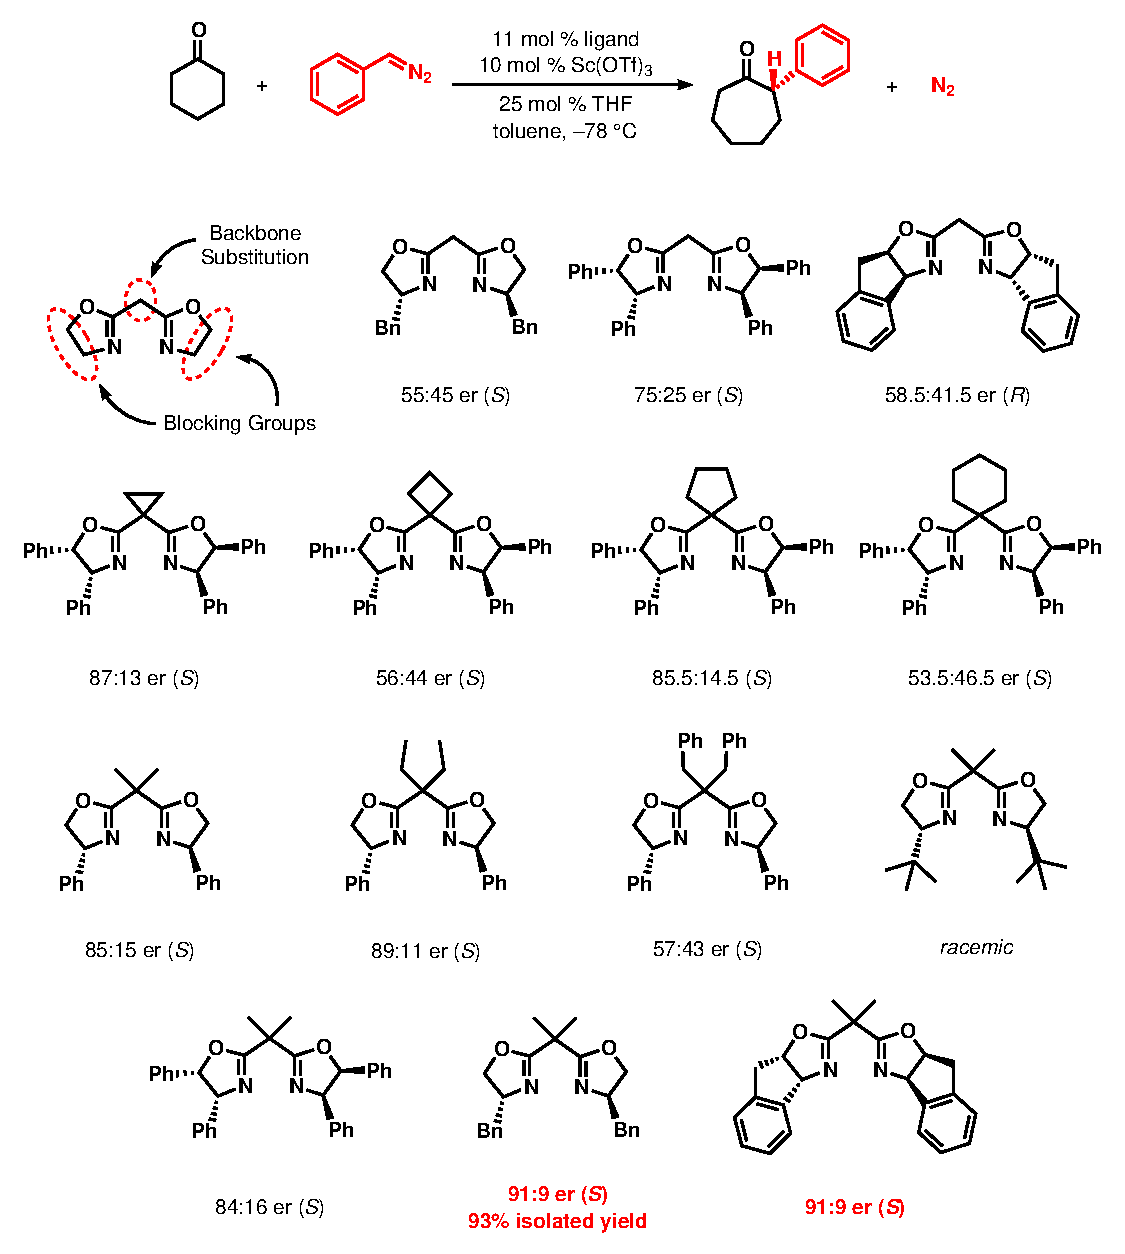
\includegraphics[scale=0.8]{chp_asymmetric/images/bigboxscreen}
  \vspace{10pt}
  \caption{Wider screen of bis(oxazoline) ligands reveals two optimum ligands.}
  \label{sch:asbigboxscreen}
\end{Scheme}
Ligand \ref{cmp:ligandac}, containing a three-membered ring backbone, showed the highest selectivity
(87:13 er) among the series, consistent with the results obtained by Davies. However, no clear trend
emerged from these data. Ligand \ref{cmp:ligandad} showed a significant drop in selectivty (55:45
er), which was regained again with ligand \ref{cmp:ligandae} (85.5:14.5 er). Purity of the ligand
may have been a determining factor, as ligand \ref{cmp:ligandad} was not as easy to crystallize
cleanly as the others in the series. Some of the ligands in \refscheme{asbigboxscreen} have also
been observed to crystallize as a solvate complex with water. Changing the blocking group to a single phenyl ring on each half and placing geminal methyl groups
on the backbone afforded comparable levels of selectivity (ligand \ref{cmp:boxasae}, 85:15 er).
Installing geminal ethyl groups on the backbone increased the selectivity slightly
(\ref{cmp:boxasaf}, 89:11 er), but with geminal benzyl groups the selectivity dropped
(\ref{cmp:ligandal}, 57:43 er). Running with \textit{tert}-leucine derived BOX \ref{cmp:boxasag}
gave completely racemic material. Curiously, phenylalanine derived BOX \ref{cmp:boxasai} and
indanyl BOX \ref{cmp:ligandaa} gave an identical 91:9 er. Material from the reaction with ligand
\ref{cmp:boxasai} was isolated in an excellent 93\% yield.

We hoped at this point that we could spend time further refining and optimizing the reaction
conditions with commercially available BOX ligand \ref{cmp:boxasai} to improve the selectivity beyond 91:9 er.
Significant effort was invested in optimizing the reaction with regard to stoichiometry, solvent, temperature, and even
various additives (\reftable{asoptimization}). Reactions run in \ce{CH2Cl2} afforded lower
selectivities, but the values were consistent regardless of changes with respect to
stoichiometry (entries 1--6). Using coordinating solvents either shut down the reaction in the case of \ce{CH3CN} (entry
7), or gave lower levels of selectivity in the case of \ce{Et2O} (entry 8). Entry 10, run in
toluene at $-$90 \degc, showed the highest selectivity at 92.5:7.5 er. The freezing point of toluene
($-$95 \degc) and the practicality of running reactions at temperatures lower than $-78$ \degc\
prevented us from looking at even lower temperatures. We looked at various additives other than THF
hoping that the appropriate additive could help solubilize or stabilize the chiral catalyst. Adding
25 mol \%  \ce{CH3CN}, \ce{Et2O}, or DME  effectively had no impact on the
selectivity (entries 11--13). Addition of 2,6-lutidine or pyridine had a detrimental effect on both
reaction kinetics and the observed enantioselectivity (entries 14, 15). This may help rationalize
why reactions with PyBOX ligand \ref{cmp:asaas} were sluggish and only moderately selective. We also
found that although THF appeared to help solubilize the catalyst mixture, it was unnecessary to
obtain high levels of selectivity (entry 17). By pre-mixing the catalyst suspension with
cyclohexanone for 15 minutes, the reaction mixture became homogeneous and afforded comparable
levels of enantioselectivity (90:10 er).
Dropping the catalyst loading to 5 mol \% had no effect on the enantioselectivity and increasing the catalyst loading to 20 mol \% gave an identical result (entries 18, 19).

\singlespacing
\ctable[
	caption = Attempts to optimize reaction conditions with bis(oxazoline) ligand \ref{cmp:boxasai}.,
	label = nowidth,
	pos = t,
	label = tbl:asoptimization,
	doinside = \footnotesize,
	botcap,
	notespar
]{ccccccccc}{
	\tnote{\textit{Conditions:} 0.1 M in solvent with 25 mol \% additive, 1.0 equiv
	phenyldiazomethane (\ref{cmp:diazoaa}). Ligand \ref{cmp:boxasai} and \ce{Sc(OTf)3} pre-complexed
	for 1.5 hrs at 23 \degc. Stirred 15 min with cyclohexanone (\ref{cmp:ascyclohexanone}) before cooling.}
	\tnote[b]{Determined by chiral SFC analysis in comparison with authentic racemic material.}
	\tnote[c]{Isolated yield after silica gel chromatography.}
	\tnote[d]{Run with 18 mg of powdered sieves and 25 mol \% THF.}
	\begin{textblock}{1}(3.1,-14) \crossrefcmp{ascyclohexanone} \end{textblock}
	\begin{textblock}{1}(6,-14) \crossrefcmp{diazoaa} \end{textblock}
	\begin{textblock}{1}(10.1,-15.95) \crossrefcmp{boxasai} \end{textblock}
	\begin{textblock}{1}(14.4,-14.2) \crossrefcmp{xaan} \end{textblock}
}{
\multicolumn{9}{c}{
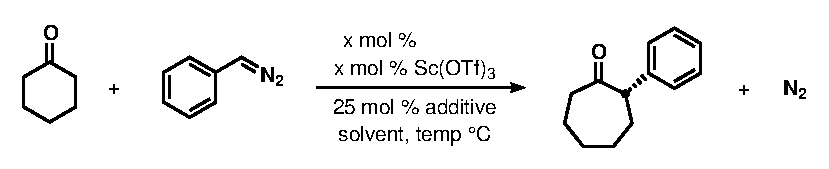
\includegraphics[scale=0.8]{chp_asymmetric/images/conditionscreenhead} \vspace{10pt}
} \\
\FL
%%% begin header line
\multirow{2}{*}{entry\tmark} &  mol \% & mol \% & equiv & \multirow{2}{*}{solvent} & \multirow{2}{*}{additive} & \multirow{2}{*}{temp (\degc)} & \multirow{2}{*}{er (\textit{R}/\textit{S})\tmark[b]} & \multirow{2}{*}{yield (\%)\tmark[c]} \NN
&\ce{Sc(OTf)3} & \ref{cmp:boxasai} & \ref{cmp:ascyclohexanone} & & & & & \ML 
%% end header line, begin data
1 & 10 & 11 & 1.1 & CH$_2$Cl$_2$ & THF & $-$78   & 84.5:15.5 (\textit{S}) & 99 \\
2\tmark[d] & 10 & 11 & 1.2 & CH$_2$Cl$_2$ & 3\AA\ sieves & $-$78   & 84:16 (\textit{S}) & 99 \\
3\tmark[d] & 10 & 11 & 1.2 & CH$_2$Cl$_2$ & 4\AA\ sieves & $-$78   & 84.5:15.5 (\textit{S}) & $>$98 \\
4 & 10 & 11 & 1.5 & CH$_2$Cl$_2$ & THF & $-$78   & 83.5:16.5 (\textit{S}) & $>$98 \\
5 & 10 & 11 & 2.0 & CH$_2$Cl$_2$ & THF & $-$78   & 83.5:16.5 (\textit{S}) & 98 \\
6 & 10 & 11 & 4.0 & CH$_2$Cl$_2$ & THF & $-$78   & 83:17 (\textit{S}) & 95 \\
7 & 10 & 11 & 1.2 & \ce{CH3CN} & $-$ & $-$78   & nd & nr \\
8 & 10 & 11 & 1.2 & Et$_2$O & $-$ & $-$78   & 75:25 (\textit{S}) & nd \\
9 & 10 & 11 & 1.2 & toluene & THF & $-$78   & 91:9 (\textit{S}) & 93 \\
\rowcolor{gray!15} 10 & 10 & 11 & 1.2 & toluene & THF & $-$90   & \textbf{92.5:7.5 (\textit{S})} &
nd \\
11 & 10 & 11 & 1.2 & toluene & CH$_3$CN & $-$78   & 90.5:9.5 (\textit{S}) & nd \\
12 & 10 & 11 & 1.2 & toluene & Et$_2$O & $-$78   & 90.5:9.5 (\textit{S}) & nd \\
13 & 10 & 11 & 1.2 & toluene & DME & $-$78   & 91:9 (\textit{S}) & nd \\
14 & 10 & 11 & 1.2 & toluene & 2,6-lutidine & $-$78   & 72.5:27.5 (\textit{S}) & nd \\
15 & 10 & 11 & 1.2 & toluene & pyridine & $-$78   & 57.5:42.5 (\textit{S}) & nd \\
16 & 10 & 11 & 1.2 & toluene & NaOTf & $-$78   & 90.5:9.5 (\textit{S}) & nd \\
17 & 10 & 11 & 1.2 & toluene & $-$ & $-$78   & 90:10 (\textit{S}) & nd \\
18 & 5 & 5.5 & 1.2 & toluene & THF & $-$78   & 90.5:9.5 (\textit{S}) & nd \\
19 & 20 & 22 & 1.2 & toluene & THF & $-$78   & 90.5:9.5 (\textit{S}) & nd \LL}
\doublespacing

\subsection{Optimal Conditions for Medium Ring Arylation}
  
After struggling to obtain higher selectivities through extensive optimization, we wanted to
glean more information about the catalyst-ligand complex. $^1$H NMR analysis of scandium BOX
mixtures showed significant line broadening and multiple additional signals, consistent with a
poorly defined and fluxional catalyst structure. By constrast, $^1$H NMR analysis of scandium PyBOX
mixtures showed cleanly resolved signals slightly offset from the uncomplexed ligand, consistent with a well
defined monomeric catalyst species in solution. Attempts to obtain a solid state structure of
scandium BOX complexes lead to a number of bis(oxazoline) triflate salt structures
(\ce{->}\ref{cmp:xabf}, \refscheme{boxtriflatesalt}). 
 \begin{Scheme}[h]
 % \centering
  \begin{textblock}{1}(9,1) 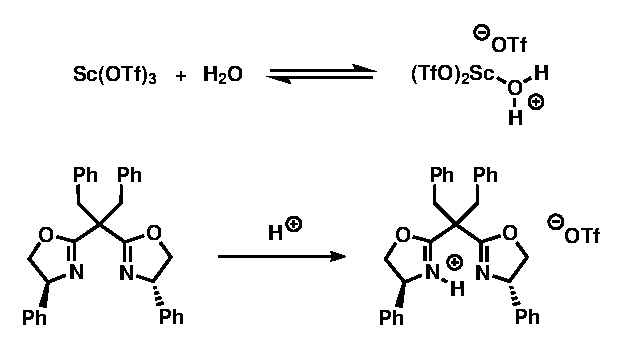
\includegraphics[scale=0.8]{chp_asymmetric/images/triflatesaltformation}
  \end{textblock}
   \begin{textblock}{1}(10.2,6.5) \crossrefcmp{ligandal} \end{textblock}
   \begin{textblock}{1}(16.6,6.5) \cmp{xabf} \end{textblock}
  \includegraphics[scale=0.35]{chp_asymmetric/images/xray/xabf_nolabels}
  \caption{Formation of a triflate salt with attempts to crystallize scandium bis(oxazoline) complexes.}
  \label{sch:boxtriflatesalt}
\end{Scheme}
It is plausible that residual water on the
\ce{Sc(OTf)3}, ligand, or in the solvents, caused water to exchange for one of the triflate ligands,
producing a Br{\o}nsted acid.\footnote{{\frenchspacing Kobayashi, S.; Nagayama, S.; Busujima, T.
Lewis Acid Catalysts Stable in Water. Correlation between Catalytic Activity in Water and Hydrolysis Constants and Exchange Rate
Constants for Substitution of Inner-Sphere Water Ligands. \textit{J. Am. Chem. Soc.} \textbf{1998},
\textit{120}, 8287-8288.}} The crystal structures of scandium PyBOX complexes contain a bound
inner-sphere water which could indicate a higher Br\o nsted basicity of the BOX ligand framework.
The increased basicity serves to funnel the Br{\o}nsted acid equilibrium to \ref{cmp:xabf}. It is
also plausible the the BOX triflate salt was simply less soluble than the corresponding PyBOX triflate salt. A control
experiment with 10 mol \% \ref{cmp:xabf} indicated that it was not a competent catalyst. These data are also consistent with experiments that showed undried \ce{Sc(OTf)3} gave variable and significantly lower levels of
enantioselectivity.


\begin{figure}[b]
\centering
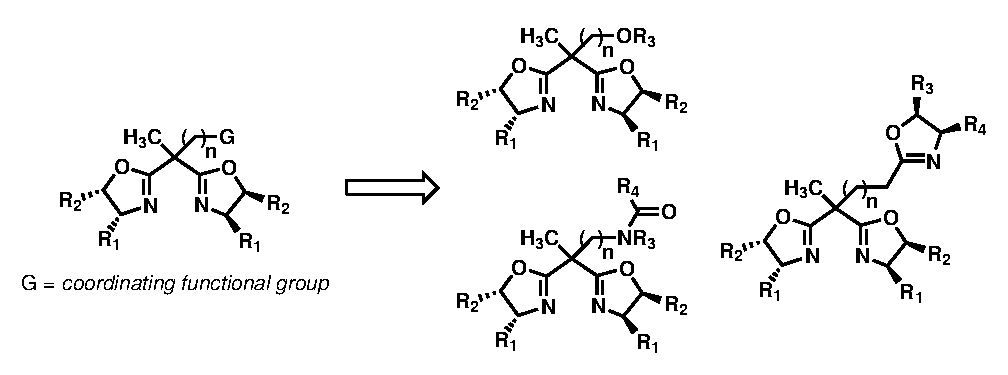
\includegraphics[scale=0.8]{chp_asymmetric/images/coordinationsitehypothesis}
  \caption{Several possibilities for the installation of a third coordinating group.}
  \label{fig:coordinationsitehypothesis}
\end{figure}
As discussed in the introduction, the PyBOX\crossref{ref:asevans} and bipyridine diol
structures\crossref{ref:askobayashistructure} from the literature revealed a 7-coordinate scandium
metal center.
Evans' well-studied scandium PyBOX catalyzed reactions all relied on a model that invoked a
two-point binding interaction between the substrate and metal, thus filling the available
coordination sites.\footnote{For a lead reference see:
{\frenchspacing Evans, D. A.; Fandrick, K. R.; Song, H. J.; Scheidt, K. A.; Xu, R. Enantioselective
Friedel-Crafts Alkylations Catalyzed by Bis(oxazolinyl)pyridine-Scandium(III) Triflate Complexes. \textit{J. Am. Chem. Soc.} \textbf{2007},
\textit{129}, 10029-10041.}} We were concerned that the BOX ligand left too much open space around
the metal center and multiple equivalents of ketone could be bound during turnover. The NMR
experiments also seemed to suggest there was a relatively weak interaction between the ligand and
scandium.  By installing another coordinating functional group in the ligand, we hypothesized that we could increase the
binding affinity for the ligand and fill more space in the coordination sphere. Our hope was that
this would force the substrate into a single binding site around the metal center and ultimately
lead to a more selective reaction. The most simple way to accomplish this would be to append the
third coordinating group to the backbone of the BOX ligand, breaking the $C_2$ symmetry.
\reffigure{coordinationsitehypothesis} illustrates several early ideas we considered. 


The first ligand we were able to access was the methyl ether substituted bis(oxazoline)
\ref{cmp:ligandam} (\refscheme{asmethyletherligand}).
Ligand \ref{cmp:ligandam} was prepared through an iterative alkylation strategy, first adding methyl
iodide and then bromoethyl methyl ether to the unsubstituted BOX framework. We were disappointed to
see a significant drop in enantioselectivity (59:41 er), but regardless, we were still motivated to
pursue alternative ligands to thoroughly test our hypothesis. The Lewis basicity of cyclohexanone and diethyl ether, as
measured by the \ce{BF3} affinity scale, are 76.36 $\pm$ 0.82 and 78.77 $\pm$ 0.38
$\frac{\mathrm{kJ}}{\mathrm{mol}}$ respectively.\footnote{Calculated from the enthalpy of
interaction between \ce{BF3}$_{\mathrm{(g)}}$ and the Lewis base. Laurence, C.; Gal, J. F.
\textit{Lewis Basicity and Affinity Scales: Data and Measurement}; John Wiley \& Sons: West Sussex,
2010; pp 85-109.} The relatively close Lewis basicities of the pendant ether functionality and
cyclohexanone could allow the cyclohexanone (present in 12 catalyst equivalents) to effectively compete for the additional coordination site.
 \begin{Scheme}[h]
  \centering
  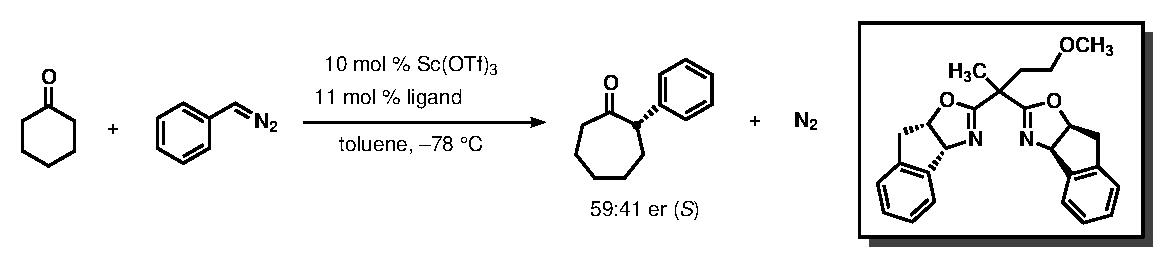
\includegraphics[scale=0.8]{chp_asymmetric/images/methyletherligand}
 \begin{textblock}{1}(17.1,-1) \cmp{ligandam} \end{textblock}
 \begin{textblock}{1}(3.2,-1) \crossrefcmp{diazoaa} \end{textblock}
  \begin{textblock}{1}(0.2,-1) \crossrefcmp{ascyclohexanone} \end{textblock}
  \begin{textblock}{1}(11.5,-1.5) \crossrefcmp{xaan} \end{textblock}
  \begin{textblock}{1}(8.0,-2.87) \crossrefcmp{ligandam} \end{textblock}
  \caption{First attempt to use a BOX ligand with third coordinating group.}
  \label{sch:asmethyletherligand}
\end{Scheme}


\begin{Scheme}[t]
 \centering
  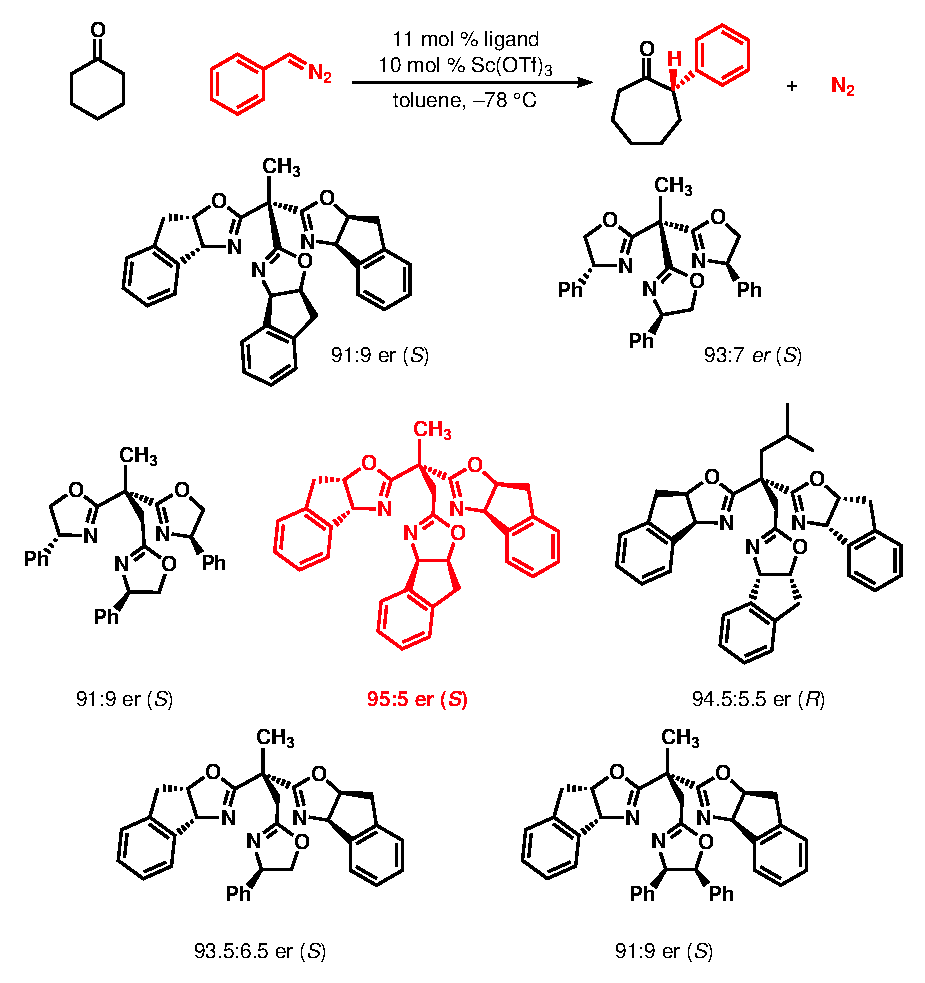
\includegraphics[scale=0.8]{chp_asymmetric/images/bigtrisoxscreen}
  \begin{textblock}{1}(3.1,-14.7) \crossrefcmp{ascyclohexanone} \end{textblock}
   \begin{textblock}{1}(6,-14.9) \crossrefcmp{diazoaa} \end{textblock}
  \begin{textblock}{1}(14,-15) \crossrefcmp{xaan} \end{textblock}
%%% row 1
\begin{textblock}{1}(4.5,-11.5) \cmp{asaax} \end{textblock}
\begin{textblock}{1}(11.7,-11.5) \cmp{asaay} \end{textblock}
%%% row 2
\begin{textblock}{1}(2,-6.5) \cmp{asaaz} \end{textblock}
\begin{textblock}{1}(6.5,-6.5) \cmp{ligandab} \end{textblock}
\begin{textblock}{1}(12.8,-6) \cmp{ligandah} \end{textblock}
%% row 3
\begin{textblock}{1}(6.5,-1) \cmp{ligandai} \end{textblock}
\begin{textblock}{1}(11.7,-1) \cmp{ligandaj} \end{textblock}
  \caption{Screen of C$_3$-symmetric and pseudo C$_3$-symmetric tris(oxazoline) ligands.}
  \label{sch:bigtrisoxscreen}
\end{Scheme}
To increase the binding ability of the third coordinating group we were drawn to the $C_3$-symmetric
tris(oxazoline) ligands reported by Bellemin-Laponnaz and Gade in 2002.\footnote{(a) {\frenchspacing
Bellemin-Laponnaz, S.; Gade, L.
H.
Three 2-Oxazolinyl Rings on One Quaternary Carbon Atom: Preparation of a Novel Tripodal Tris(oxazolinyl)
Ligand and the Tetrameric Molecular Structure of its CuI Complex. \textit{Chem. Commun.}
\textbf{2002}, 1286-1287.} (b) {\frenchspacing Gade, L. H.; Bellemin-Laponnaz, S. S. Exploiting
Threefold Symmetry in Asymmetric Catalysis: The Case of Tris(oxazolinyl)ethanes (``trisox'').
\textit{Chem. Eur. J.} \textbf{2008}, \textit{14}, 4142-4152.}} The $C_3$-symmetric TOX ligands
\ref{cmp:asaax} and \ref{cmp:asaay} were synthesized according to the reported procedures and tested
under our standard reaction conditions (\refscheme{bigtrisoxscreen}). The
indanyl TOX ligand \ref{cmp:asaax} afforded the same selectivity observed with the parent BOX
ligand \ref{cmp:ligandaa} (91:9 er). We were excited to see a
slight increase in selectivity with phenylglycine-derived TOX ligand \ref{cmp:asaay} (93:7 er).  We
also prepared several pseudo $C_3$-symmetric TOX ligands first introduced by Tang in
2002.\footnote{(a) {\frenchspacing Zhou, J.; Tang, Y. Sidearm Effect:
improvement of the Enantiomeric Excess in the Asymmetric Michael Addition of Indoles to Alkylidene Malonates. \textit{J. Am. Chem.
Soc.} \textbf{2002}, \textit{124}, 9030-9031.} (b) {\frenchspacing Zhou, J.; Tang, Y. The
Development and Application of Chiral Trisoxazolines in Asymmetric Catalysis and Molecular
Recognition. \textit{Chem. Soc. Rev.} \textbf{2005}, \textit{34}, 664-676.}} The phenyl blocking
group (ligand \ref{cmp:asaaz}) delivered a 91:9 er, while the indanyl ligand \ref{cmp:ligandab}
finally gave a synthetically viable 95:5 er. We wanted to probe the effect of changing the backbone
substitution and nature of the third coordinating group within the context of the pseudo
C$_3$-symmetric ligand framework. Adding an isobutyl group to the backbone (ligand
\ref{cmp:ligandah}) afforded nearly identical selectivity (94.5:5.5 er) as ligand
\ref{cmp:ligandab}, suggesting the ligand likely binds in a tripodal fashion, placing the alkyl chain away from the site of
reaction.\footnote{For a tripodal structure of TOX bound \ce{ScCl3} (not found in the CSD search)
see:
{\frenchspacing Gade, L.
H.; Marconi, G.; Dro, C.; Ward, B.
D.; Poyatos, M.; Bellemin-Laponnaz, S.; Wadepohl, H.; Sorace, L.; Poneti, G. Shaping and Enforcing Coordination
Spheres: The Implications of $C_3$ and $C_1$ Chirality in the Coordination Chemistry of 1,1,1-Tris(oxazolinyl)ethane (``Trisox''). \textit{Chem. Eur. J.} \textbf{2007}, \textit{13}, 3058-3075.}} The nature of the third coordinating group was important to obtaining high selectivity.
Without the indanyl blocking group  (ligands \ref{cmp:ligandai} and \ref{cmp:ligandaj}) selectivity
dropped.
\vspace{-8pt}
\begin{singlespace}
\ctable[
	caption = Scope of asymmetric $\alpha$-arylation by diazoalkane ring expansion.,
	label = nowidth,
	pos = p,
	label = tbl:assubstrates,
	doinside = \footnotesize,
	botcap,
	notespar
]{>{\centering}m{.6cm}>{\centering}m{1.4cm}>{\centering}m{2cm}>{\centering}m{1cm}>{\centering}m{1.5cm}>{\centering}m{2.4cm}>{\centering}m{1.2cm}>{\centering}m{1.0cm}}{
%	\begin{textblock}{1}(18.2,-23.5) \crossrefcmp{ligandaa} \end{textblock}
	\begin{textblock}{1}(14,-23.5) \crossrefcmp{ligandab} \end{textblock}
\tnote{Yield over two steps from the aldehyde based on $^{19}$F NMR titration with
\textit{o}-\ce{FC6H4CO2H}.}
\tnote[b]{Isolated yield after silica gel chromatography.}
\tnote[c]{By chiral SFC analysis in comparison with authentic racemic material.}
\tnote[d]{Purified by extraction into hexanes.}
\tnote[e]{Run at $-$45 \degc.}
}{
\multicolumn{8}{c}{
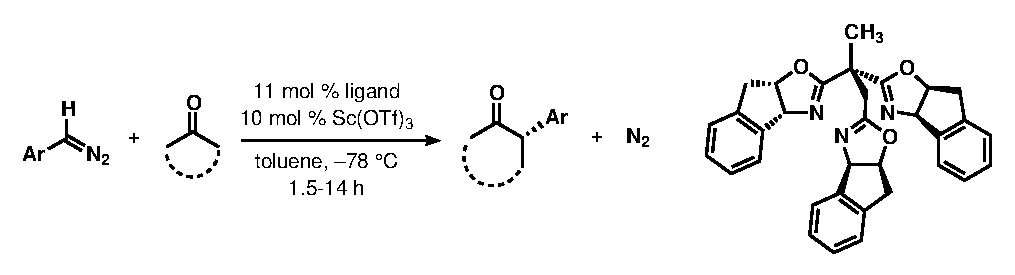
\includegraphics[scale=0.8]{chp_asymmetric/images/substratetablehead} \vspace{0pt}
} \\
\FL
%%% begin header line
\multirow{2}{*}{entry} & \multirow{2}{*}{electrophile} & \multirow{2}{*}{nucleophile} &
\multirow{2}{*}{ligand} & diazoalkane & insertion & \multirow{2}{*}{yield (\%)\tmark[b]} &
\multirow{2}{*}{er\tmark[c]} \NN &&&&yield (\%)\tmark &product&& \ML
%% end header line, begin data
1\tnote[d] & \includegraphics[scale=0.8]{chp_asymmetric/images/cyclobutanone} &
\includegraphics[scale=0.8]{chp_asymmetric/images/phenyldiazomethane} \crossrefcmp{diazoaa} &
\ref{cmp:ligandab} & 75 & \includegraphics[scale=0.8]{chp_asymmetric/images/xaamnobox} \cmp{xaam} & $>$98 & 85.5:14.5 \NN
2 & \includegraphics[scale=0.8]{chp_asymmetric/images/cyclopentanone} &
\includegraphics[scale=0.8]{chp_asymmetric/images/phenyldiazomethane} \crossrefcmp{diazoaa} &
\ref{cmp:ligandab} & 75 & \includegraphics[scale=0.8]{chp_asymmetric/images/phenylhexanone} \cmp{asphenylcyclohex} & $<$2 & nd
\NN & \includegraphics[scale=0.8]{chp_asymmetric/images/cyclohexanone} &
\includegraphics[scale=0.8]{chp_asymmetric/images/diazolabelg} &  &  &
\includegraphics[scale=0.8]{chp_asymmetric/images/heptanonegeneric} &  &  \NN
3 & & \multicolumn{1}{l}{\crossrefcmp{diazoaa} G = H} & \ref{cmp:ligandab} & 75 &
\multicolumn{1}{l}{\crossrefcmp{xaan} G = H} & 94 & 95:5\NN 4 & & \multicolumn{1}{l}{\cmp{diazoah} G
= \textit{p}-CH$_3$} & \ref{cmp:ligandab} & 80 & \multicolumn{1}{l}{\cmp{xaao} G =
\textit{p}-CH$_3$} & 96 & 94:6 \NN 5 & & \multicolumn{1}{l}{\cmp{diazoai} G = \textit{m}-Br} &
\ref{cmp:ligandab} & 68 & \multicolumn{1}{l}{\cmp{xaap} G = \textit{m}-Br} & $>$98 & 94.5:5.5 \NN
 & \includegraphics[scale=0.8]{chp_asymmetric/images/cycloheptanone} &
\includegraphics[scale=0.8]{chp_asymmetric/images/diazolabelg} &  &  &
\includegraphics[scale=0.8]{chp_asymmetric/images/octanonegeneric} &  &  \NN
6 & & \multicolumn{1}{l}{\crossrefcmp{diazoaa} G = H} & \ref{cmp:ligandab} & 75 &
\multicolumn{1}{l}{\cmp{xaal} G = H} & 99 & 98:2 \NN
7 & & \multicolumn{1}{l}{\crossrefcmp{diazoah} G = \textit{p}-CH$_3$} & \ref{cmp:ligandab} & 80 &
\multicolumn{1}{l}{\cmp{xaau} G = \textit{p}-CH$_3$} & $>$98 & 98.5:1.5 \NN
8 & & \multicolumn{1}{l}{\cmp{diazoae} G = \textit{m}-OCH$_3$} & \ref{cmp:ligandab} & 64 &
\multicolumn{1}{l}{\cmp{xaas} G = \textit{m}-OCH$_3$} & $>$98 & 97:3 \NN
9 & & \multicolumn{1}{l}{\cmp{diazoad} G = \textit{p}-CF$_3$} & \ref{cmp:ligandab} & 73 &
\multicolumn{1}{l}{\cmp{xaar} G = \textit{p}-CF$_3$} & 78 & 98:2 \NN
10 & & \multicolumn{1}{l}{\cmp{diazoac} G = \textit{o}-Br} & \ref{cmp:ligandaa} & 74 &
\multicolumn{1}{l}{\cmp{xaaq} G = \textit{o}-Br} & 85 & 92.5:7.5 \NN
11 & & \multicolumn{1}{l}{\cmp{diazoaf} G = \textit{o}-CH$_3$} & \ref{cmp:ligandaa} & 63 &
\multicolumn{1}{l}{\cmp{xaat} G = \textit{o}-CH$_3$} & 97 & 93.5:6.5 \NN
12 &  &
\includegraphics[scale=0.8]{chp_asymmetric/images/onenapdiazo} \cmp{diazoag} & \ref{cmp:ligandaa}  &
63 & \includegraphics[scale=0.8]{chp_asymmetric/images/xaavnobox} \cmp{xaav} & 94  & 93:7  \NN
 13\tnote[e] & \includegraphics[scale=0.8]{chp_asymmetric/images/cyclooctanone} &
\includegraphics[scale=0.8]{chp_asymmetric/images/phenyldiazomethane} \crossrefcmp{diazoaa} &
\ref{cmp:ligandab} & 75 &
\includegraphics[scale=0.8]{chp_asymmetric/images/xaawnobox} \cmp{xaaw} & $>$98 & 93:7    \LL}
\end{singlespace}
With high levels of enantioselectivity for the model substrate now attainable using ligand
\ref{cmp:ligandab}, we started to evaluate the reaction scope with regard to cycloalkanone and
diazoalkane (\reftable{assubstrates}). Homologation of cyclobutanone with
phenyldiazomethane delivered \ref{cmp:xaam} in a lower 85.5:14.5 er (entry 1). The
product was purified through an aqueous workup and hexane extraction because of the tendency for $\alpha$-aryl cyclopentanones
to racemize on silica.\crossref{ref:asshitertiary} As anticipated, the reaction with cyclopentanone
gave a complex mixture of products derived from overhomologation (entry 2). The desired insertion product \ref{cmp:asphenylcyclohex} was
significantly more reactive than the starting
cyclopentanone.\crossref{ref:asgutscherev}$^,$\footnote{{\frenchspacing Maruoka, K.; Concepcion, A.
B.; Yamamoto, H. Selective Homologation of Ketones and Aldehydes with Diazoalkanes Promoted by
Organoaluminum Reagents. \textit{Synthesis} \textbf{1994}, 1283-1290.} \label{ref:asyamamotohomo}}
Alkyl and halogen groups on the diazoalkane were well tolerated, providing \ref{cmp:xaao} and \ref{cmp:xaap} in nearly identical
selectivity to \ref{cmp:xaan} (entries 4 and 5). We were very pleased to see that homologation of
cycloheptanone delivered products with even higher selectivity than that observed with cyclohexanone (entries
6--9). The yield in entry 9 was slightly depressed due to the lower nucleophilicity of diazoalkane
\ref{cmp:diazoad}, which caused the reaction to progress slowly and not reach full conversion even
after 14 hours.
Use of more hindered \textit{ortho}-substituted nucleophiles \ref{cmp:diazoac} and \ref{cmp:diazoaf}
resulted in diminished reactivity with TOX ligand \ref{cmp:ligandab} at the cold temperatures needed
to ensure high enantiocontrol. In these cases, however, the parent BOX ligand \ref{cmp:ligandaa} 
restored a rapid and smooth merger of the reactants presumably due to a less crowded Sc coordination
sphere (\ref{cmp:xaaq} and \ref{cmp:xaat}, 93:7 er, entries 10 and 11). The same trend was observed
when 1-naphthyldiazomethane (\ref{cmp:diazoag}) was used to prepare aryloctanone \ref{cmp:xaav}
(93:7 er, entry 12). Reaction of cyclooctanone proceeded slowly, but full conversion and a 93:7 er was
obtained after 14 hours at $-$45 \degc\  (entry 13). Depending on the ring size, the stoichiometry
was modified to maximize conversion and minimize overhomologation. For entries 3--5,
overhomologation of the cycloheptanone products had been observed in previous studies, therefore
the diazoalkane was used as the limiting reagent. A slight excess (1.2 equivalents) of
cyclohexanone was added to ensure the diazoalkane was completely consumed before having an
opportunity to react with the products. In entries 6--13, overhomologation was not a concern and an
excess of the diazoalkane was used (1.2--1.4 equivalents) to ensure high conversion. Reactions with
larger cycloalkanones and \textit{ortho}-substituted diazoalkanes proceeded slower than 6--
and 4-membered ring expansions, which lead to slight decomposition of the diazoalkane in the
reaction time frame.

\begin{Scheme}[b]
  \centering
  \begin{textblock}{1}(3.5,3.2) \crossrefcmp{diazoaa} \end{textblock}
   \begin{textblock}{1}(8.4,1.75) \crossrefcmp{ligandab} \end{textblock}
   \begin{textblock}{1}(11.8,2.4) \crossrefcmp{xaal} \end{textblock}
  \includegraphics[scale=0.8]{chp_asymmetric/images/heptscaleup}
   \begin{textblock}{1}(13.8,-1.5) \crossrefcmp{ligandab} \end{textblock}
  \caption{Scale-up of cycloheptanone homologation with lower catalyst loading.}
  \label{sch:asscaleup}
\end{Scheme}
The asymmetric homologation reactions could be scaled to provide preparative quantities of
enantioenriched products. We could also drop the catalyst loading to 5 mol \% and still obtain high
yields and selectivies in a reasonable timeframe by increasing the reaction concentration. After
6 hours, aryl octanone \ref{cmp:xaal} was isolated in 94\% yield (235 mg) and 97:3 er with 5 mol \%
\ce{Sc(OTf3)} and 5.5 mol \% ligand \ref{cmp:ligandab} (\refscheme{asscaleup}). Attempts to drop the
catalyst loading further resulted in incomplete conversion even after prolonged reaction times. With
2.5 mol \% \ce{Sc(OTf)3}, \ref{cmp:xaal} was recovered in a 50\% distilled yield (5 mmol scale) and
95:5 er after 22 hours.
 
 \begin{Scheme}[t]
  \centering
   \begin{textblock}{1}(2.5,4.5) \crossrefcmp{xaal} \end{textblock}
   \begin{textblock}{1}(10,3.7) \cmp{xabc} \end{textblock}
      \begin{textblock}{1}(18,1.2) \cmp{xabe} \end{textblock}
   \begin{textblock}{1}(18,5.8) \cmp{xabd} \end{textblock}
  \includegraphics[scale=0.8]{chp_asymmetric/images/absolutestereochem}
  \caption{NMR-based proof of absolute stereochemistry for \ref{cmp:xaal}.}
  \label{sch:asabsolutestereochem}
\end{Scheme}
The absolute stereochemistry of \ref{cmp:xaan} (entry 3,
\reftable{assubstrates}) was assumed to be (\textit{S}) by comparing optical rotation data with that
reported in the asymmetric protonation literature.\footnote{The absolute stereochemistry given in
reference \ref{ref:asyanagisawa} was determined by ``analogy''.}
In order to develop a stereochemical model we needed to confirm the absolute stereochemistry of our medium ring cycloalkanones.
While \ref{cmp:xaal} was obtained as a solid, attempts to crystallize it directly
or various derivatives was largely unsuccessful. We decided to reduce \ref{cmp:xaal} and attempt an
NMR based stereoproof using $\alpha$-acetylmandelate esters
(\refscheme{asabsolutestereochem}).\footnote{{\frenchspacing Trost, B.
M.; Belletire, J. L.; Godleski, S.; McDougal, P. G.; Balkovec, J. M.; Baldwin, J. J.; Christy, M. E.; Ponticello, G. S.; Varga, S. L.; Springer, J. P. On the Use of the \textit{O}-Methylmandelate Ester for Establishment of Absolute Configuration of Secondary Alcohols. \textit{J. Org. Chem.} \textbf{1986}, \textit{51}, 2370-2374.}} A sample of
optically enriched \ref{cmp:xaal} ($>$95:5 er) was reduced with Red-Al in toluene at $-78$ \degc\ to
deliver the \textit{cis}-cyclooctanol \ref{cmp:xabc} in 2.5:1 dr and a 66\% isolated yield of
the major diastereomer.\footnote{Racemic material was converted to the \textit{p}-\ce{NO2} benzoate
ester and crystallized to confirm the relative stereochemistry. See the experimental section and
appendix for details.} Initial attempts to use K-selectride resulted in a more diastereoselective
reduction, but the recovered cyclooctanol was completely racemic. Coupling with (\textit{R})-- and
(\textit{S})-$\alpha$-acetylmandelic acid provided sufficient quantities of $\alpha$-acetylmandelate esters \ref{cmp:xabe} and \ref{cmp:xabd} for NMR analysis. The chemical shifts of the protons in
both diastereomers were assigned through the COSY and HSQC 2D spectra because of overlapping
resonances. The protons indicated as H$_\mathrm{a}$ are diastereotopic and careful analysis of the
spectra was required to ensure the correct signals in \ref{cmp:xabe} and \ref{cmp:xabd} were being compared.
Regardless of how the data are analyzed, the proton signals associated with the carbon bearing
H$_\mathrm{a}$ and H$_\mathrm{a'}$ show a significant upfield shift in the \textit{R} ester,
consistent with an anisotropic shielding effect from the ester conformation shown in structure \ref{cmp:xabe}. Likewise, the
proton labelled H$_\mathrm{b}$ was shielded in the \textit{S} ester \ref{cmp:xabd}. The data used to
make the determination are given in \reftable{asmandelatestereoproof}. From these data, absolute
stereochemistry for the secondary alcohol was assigned as \textit{S}, confirming that the $\alpha$-aryl stereochemistry was also \textit{S}.
\begin{table}[h]
{\small
\begin{tabular}{cccccc}
\toprule
proton & $\delta_S$ (ppm) & $\delta_R$ (ppm) & $\delta_{S-R} (ppm)$ & Hz & group \\
\midrule
H$_\mathrm{a}$ & 1.87 & 1.62 & $+$0.25 & $+$125 & \textbf{\color{red}{A}} \\
H$_\mathrm{c'}$ & 1.78 & 1.58 & $+$0.20 & $+$100 & \textbf{\color{red}{A}} \\
H$_\mathrm{a'}$ & 1.94 & 1.74 & $+$0.20 & $+$100 & \textbf{\color{red}{A}} \\
H$_\mathrm{c}$ & 1.64 & 1.52 & $+$0.12 & $+$60 & \textbf{\color{red}{A}} \\
H$_\mathrm{d'}$ & 2.06 & 2.11 & $-$0.05 & $-$25 & \textbf{\color{blue}{B}} \\
H$_\mathrm{b}$ & 2.96 & 3.10 & $-$0.14 & $-$70 & \textbf{\color{blue}{B}} \\
H$_\mathrm{d}$ & 1.69 & 1.83 & $-$0.14 & $-$70 & \textbf{\color{blue}{B}} \\
\bottomrule
\end{tabular}
}
 \begin{textblock}{1}(13.5,-3.2)  \includegraphics[scale=0.8]{chp_asymmetric/images/prooflabels}
 \end{textblock}
\caption{Data used to determine the absolute stereochemistry of \ref{cmp:xaal}.}
\label{tbl:asmandelatestereoproof}
\end{table}


Before proposing a stereochemical model, we also wanted to gather information about
the approach trajectory of the diazoalkane nucleophile. We designed a diastereoselective
homologation reaction similar to the experiment performed by Yamamoto in 1994
(\refscheme{yamamotodiastereo}, page \pageref{sch:yamamotodiastereo}).\crossref{ref:asyamamotohomo}
Treatment of 4-\textit{tert}-butylcyclohexanone with diazo \ref{cmp:diazoah} in the presence of 10
mol \% \ce{Sc(OTf)3} lead to the highly diastereoselective formation of \textit{trans} insertion
product ($\pm$)-\ref{cmp:xaay} (96.5:3.5 dr, by achiral GC analysis,
\refscheme{asdiastereoselective}).
Crystallization of the major diastereomer confirmed the \textit{trans} relative stereochemistry.
Consistent with the reported data in the literature, the observed diastereoselectivity with
stoichiometric trimethylaluminum was lower (82:18 dr).\crossref{ref:asyamamotohomo} With 10 mol \%
\ce{Sc(OTf)3} and ligand \ref{cmp:ligandab}, an enantio-- and diastereoselective reaction delivered
\ref{cmp:xaay} in 93:7 dr with 92.5:7.5 er for the major diastereomer. The diastereoselectivity can
be rationalized by invoking a model with an axial approach of the diazoalkane. The diazoalkane
likely approaches in an orientation that places the proton over the 6-membered ring to minimize
penalizing steric interactions between the aryl group and ring. The principle of least motion
states that \textit{``those elementary reactions will be favored that involve the least change in
atomic position and electronic configuration''}.\footnote{{\frenchspacing Tee, O. S. Application of
the Principle of Least Motion to Organic Reactions. A Generalized Approach. \textit{J. Am. Chem.
Soc.} \textbf{1969}, \textit{91}, 7144-7149.}} Assuming that the betaine intermediate
undergoes a least motion collapse directly from the drawn conformation and without \ce{C-C} bond
rotation, the observed diastereomer can be correctly predicted. A 120$^{\circ}$ rotation
after the diazoalkane has added would lead to the other diastereomer. However, it would introduce
significant torsional strain. Adding the other enantioface of the diazoalkane in the same orientation (Ar and N$_2$ swapped, H over ring) still predicts to the same relative stereochemistry. \begin{Scheme}[t]
 % \centering
 \begin{textblock}{1}(5,4.5) \crossrefcmp{diazoah} \end{textblock}
 \begin{textblock}{1}(11.5,1.9) \cmp{xaaz} \end{textblock}
  \begin{textblock}{1}(11.5,6.5) \cmp{xaay} \end{textblock}
   \begin{textblock}{1}(12.2,0.2)
   \includegraphics[scale=0.35]{chp_asymmetric/images/xray/xaax_nolabels} \end{textblock}
  \includegraphics[scale=0.8]{chp_asymmetric/images/diastereoselective}
  \caption{Diastereo-- and enantioselective insertion reactions with
  4-\textit{tert}-butylcyclohexanone.}
  \label{sch:asdiastereoselective}
\end{Scheme}

A stereochemical model to predict the absolute stereochemistry was designed based on the
aforementioned principles (\refscheme{stereochemicalmodel}). The enantioselectivity of the reaction
is most likely derived from control over the orientation with which the diazoalkane adds to
the symmetric cycloalkanone substrate. The counterions (omitted for clarity) and ligand
\ref{cmp:ligandab} establish a chiral pocket that forces the diazoalkane to enter over the open side of the ligand (from left).
The diazoalkane adds in an orientation such that the aryl group is directed away out the back of
the chiral pocket and the proton is positioned over the cycloalkanone ring. The newly formed
\ce{C-C} bond resides initially in an axial position, and then concerted collapse with expulsion of nitrogen gas delivers the \textit{S} product. This prediction was in agreement with the observed selectivity.
 \begin{Scheme}[h]
  \centering
   \begin{textblock}{1}(18,3.2) \crossrefcmp{xaaa} \end{textblock}
  \includegraphics[scale=0.8]{chp_asymmetric/images/stereochemicalmodel}
  \caption{Stereochemical model correctly predicts the (\textit{S}) enantiomer of product.}
  \label{sch:stereochemicalmodel}
\end{Scheme}
 
\pagebreak
\section{Additional Developments}
\subsection{Synthesis of a Novel $\pi$-Extended Bis(oxazoline) Ligand}

\begin{figure}[b]
  \centering
   \begin{textblock}{1}(10.2,2.7) \crossrefcmp{ligandaa} \end{textblock}
   \begin{textblock}{1}(1.1,1.3) \cmp{asaba} \end{textblock}
   \begin{textblock}{1}(3.2,2.6) \cmp{asabb} \end{textblock}
   \begin{textblock}{1}(15,2.7) \cmp{xlaai} \end{textblock}
  \includegraphics[scale=0.8]{chp_asymmetric/images/indanylchart}
  \caption{\textit{cis}-Amino indanol \ref{cmp:asaba} and derivatives.}
  \label{fig:asindanylchart}
\end{figure}
Chiral vicinal amino alcohols, both natural and fully synthetic, represent an exceptionally
important class of small molecules. Amino alcohols have long been utilized in asymmetric catalysis
as ligands themselves\footnote{(a) {\frenchspacing Oguni, N.; Omi, T. Enantioselective Addition of Diethylzinc to
Benzaldehyde Catalyzed by a Small Amount of Chiral 2-Amino-1-Alcohols. \textit{Tetrahedron Lett.}
\textbf{1984}, \textit{25}, 2823-2824.} (b) {\frenchspacing Kitamura, M.; Suga, S.; Kawai, K.;
Noyori, R. Catalytic Asymmetric Induction. Highly Enantioselective Addition of Dialkylzincs to
Aldehydes. \textit{J. Am. Chem. Soc.} \textbf{1986}, \textit{108}, 6071-6072.} (c) {\frenchspacing
Kitamura, M.; Okada, S.; Suga, S.; Noyori, R. Enantioselective Addition of Dialkylzincs to Aldehydes
Promoted by Chiral Amino Alcohols. Mechanism and Nonlinear Effect. \textit{J. Am. Chem. Soc.}
\textbf{1989}, \textit{111}, 4028-4036.}} or as precursors to various ligand
classes.\footnote{{\frenchspacing Yoon, T. P.; Jacobsen, E. N. Privileged Chiral Catalysts.
\textit{Science} \textbf{2003}, \textit{299}, 1691-1693.}} As chemists continue to expand the scope
of available catalytic enantioselective transformations, the need for new and rationally designed
synthetic amino alcohols is justified. The \textit{cis}-substituted amino indanol \ref{cmp:asaba}
(\reffigure{asindanylchart}), for instance, was first developed as a subunit of the orally active
HIV protease inhibitor indinavir\footnote{{\frenchspacing Senanayake, C. H. Applications of \textit{cis}-1-Amino-2-indanol
in Asymmetric Synthesis. \textit{Aldrichimica Acta} \textbf{1998}, \textit{31(1)}, 3-15.}}
(Crixivan\regtm). Davies, Senanayake, and others in process research at Merck went on to establish
the derived oxazolidinone \ref{cmp:asabb} and bis(oxazoline) ligands\footnote{For pioneering
studies with BOX ligands see: (a) {\frenchspacing Lowenthal, R. E.; Abiko, A.; Masamune, S.
Asymmetric Catalytic Cyclopropanation of Olefins: Bis-Oxazoline Copper Complexes. \textit{Tetrahedron Lett.}
\textbf{1990}, \textit{31}, 6005-6008.} (b) {\frenchspacing M\"{u}ller, D.; Umbricht, G.; Weber, B.;
Pfaltz, A. C$_2$-Symmetric 4,4�,5,5'-Tetrahydrobi(oxazoles) and
4,4',5,5'-Tetrahydro-2,2'-methylenebis[oxazoles] as Chiral Ligands for Enantioselective Catalysis.
\textit{Helv. Chim. Acta.} \textbf{1991}, \textit{74}, 232-240.} (c) {\frenchspacing Evans, D. A.;
Woerpel, K. A.; Hinman, M. M.; Faul, M. M. Bis(oxazolines) as Chiral Ligands in Metal-Catalyzed
Asymmetric Reactions. Catalytic, Asymmetric Cyclopropanation of Olefins. \textit{J. Am. Chem. Soc.}
\textbf{1991}, \textit{113}, 726-728.} (d) {\frenchspacing Corey, E. J.; Imai, N.; Zhang, H. Y.
Designed Catalyst for Enantioselective Diels-Alder Addition from a C$_2$-Symmetric Chiral
Bis(oxazoline)-Fe(III) Complex. \textit{J. Am. Chem. Soc.} \textbf{1991}, \textit{113}, 728-729.}}
such as \ref{cmp:ligandaa} as highly effective and tunable chiral controllers for catalytic
Diels-Alder reactions.\crossref{ref:asdaviesdielsalder}$^,$\footnote{(a) {\frenchspacing Davies, I.
W.; Senanayake, C. H.; Castonguay, L.; Larsen, R. D.; Verhoeven, T. R.; Reider, P. J. Highly
Diastereoselective Diels-Alder Reaction Mediated by a Chiral Auxiliary Derived from Amino Indanol:
The Role of Conformation on Diastereoselectivity. \textit{Tetrahedron Lett.} \textbf{1995},
\textit{36}, 7619-7622.} (b) {\frenchspacing Davies, I. W.; Senanayake, C. H.; Larsen, R. D.;
Verhoeven, T. R.; Reider, P. J. Application of Indane-derived C$_2$-Symmetric Bis(oxazolines) in
Two-point Binding Asymmetric Diels-Alder Reactions. \textit{Tetrahedron Letters} \textbf{1996},
\textit{37}, 1725-1726.} (c) {\frenchspacing Davies, I. W.; Gerena, L.; Cai, D.; Larsen, R. D.;
Verhoeven, T. R.; Reider, P. J. A Conformational Toolbox of Oxazoline Ligands. \textit{Tetrahedron
Lett.} \textbf{1997}, \textit{38}, 1145-1148.} \label{ref:asdaviesbiglist}} The superiority of these
systems relative to those based on phenylglycinol draws from the fact that the indane ring prevents free rotation about the
\ce{C-Ph} bond, enforcing conformational rigidity.\footnote{{\frenchspacing Sibi, M. P.; Ji, J.
Practical and Efficient Enantioselective Conjugate Radical Additions. \textit{J. Org. Chem.}
\textbf{1997}, \textit{62}, 3800-3801.} See references \ref{ref:asdaviesdielsalder} and
\ref{ref:asdaviesbiglist} also.} Our success with BOX and TOX ligands derived from amino indanol
\ref{cmp:asaba} inspired us to develop a new $\pi$-extended amino alcohol (\ref{cmp:xlaai}) to
address some of the enantioselectivity issues with smaller ring homologations (entry 1,
\reftable{assubstrates}, page \pageref{tbl:assubstrates}).\footnote{{\frenchspacing Rendina, V. L.; Goetz, S. A.;
Neitzel, A. E.; Kaplan, H. Z.; Kingsbury, J. S. Scalable Synthesis of a New Enantiomerically Pure $\pi$-Extended Rigid Amino
Indanol.
\textit{Tetrahedron Lett.} \textbf{2012}, \textit{53}, 15-18.}} We hypothesized that the lower
selectivity observed for  4\ce{->}5 ring expansions was the result of more conformational
freedom of the smaller cycloalkanone within the chiral pocket. By extending the ligand blocking
groups, we hoped to minimize this flexibility and increase enantioselectivity in the arguably more
synthetically useful cyclobutanone homologations.\crossref{ref:asbuchwaldarylation} 
\begin{Scheme}[h]
  \centering
   \begin{textblock}{1}(1.9,2) \cmp{xlaak} \end{textblock}
  \begin{textblock}{1}(6,3) \crossrefcmp{xlaai} \end{textblock}
   \begin{textblock}{1}(9.5,3) \cmp{xlaae} \end{textblock}
    \begin{textblock}{1}(13.5,3) \cmp{xlaad} \end{textblock}
    \begin{textblock}{1}(17,3) \cmp{asabc} \end{textblock}
  \includegraphics[scale=0.8]{chp_asymmetric/images/ligandretro}
  \caption{Retrosynthetic analysis for new $\pi$-extended bis(oxazoline) ligand.}
  \label{sch:asligandretro}
\end{Scheme}



\refscheme{asligandretro} shows a retrosynthesis for the new $\pi$-extended BOX ligand
\ref{cmp:xlaak}. The required 3\textit{H}-benz[\textit{e}]indene (\ref{cmp:xlaae}) was a known
material, but it forms in low yield as a byproduct of the pyrolysis of 2'-methyl-biphenyl-2,3-dicarboxylic anhydride.\footnote{{\frenchspacing Brown, R.; Eastwood, F.; Smith, C.
Pyrolytic Generation of Aryne and Exocyclic Carbene Species: Trapping by an Adjacent
\textit{o}-Tolyl Group. \textit{Aust. J. Chem.} \textbf{1992}, \textit{45}, 1315-1320.}} As such, it
seemed appropriate to target \ref{cmp:xlaae} more efficiently by a simple reduction-elimination
sequence on the known ketone \ref{cmp:xlaad}. In opening attempts to prepare \ref{cmp:xlaad} in one
flask from acryloyl chloride and naphthalene by tandem AlCl$_3$-mediated Friedel-Crafts acylation
and Nazarov cyclization,\footnote{{\frenchspacing Dietrich, U.; Hackmann, M.; Rieger, B.; Klinga,
M.; Leskel\"{a}, M. Control of Stereoerror Formation with High-Activity ``Dual-Side'' Zirconocene
Catalysts: A Novel Strategy To Design the Properties of Thermoplastic Elastic Polypropenes. \textit{J. Am. Chem. Soc.} \textbf{1999}, \textit{121}, 4348-4355.}} tedious column chromatography was needed and the yield was only modest.
Other literature procedures called for expensive starting materials and did not scale well in our
hands.\footnote{(a) {\frenchspacing Hulin, B.; Koreeda, M. A Convenient, Mild Method for the
Cyclization of 3-- and 4-Arylalkanoic Acids \textit{via} Their Trifluoromethanesulfonic Anhydride
Derivatives. \textit{J. Org. Chem.} \textbf{1984}, \textit{49}, 207-209.} (b) {\frenchspacing Kita,
Y.; Higuchi, K.; Yoshida, Y.; Iio, K.; Kitagaki, S.; Ueda, K.; Akai, S.; Fujioka, H.
Enantioselective Total Synthesis of a Potent Antitumor Antibiotic, Fredericamycin A. \textit{J. Am.
Chem. Soc.} \textbf{2001}, \textit{123}, 3214-3222.} (c) {\frenchspacing Wu, X.; Nilsson, P.;
Larhed, M. Microwave-Ehanced Carbonylative Generation of Indanones and 3-Acylaminoindanones.
\textit{J. Org. Chem.} \textbf{2005}, \textit{70}, 346-349.} \label{ref:astlalternatives}}
Therefore, an alternative route was developed from inexpensive 2-methylnaphthalene
(\ref{cmp:asabc}, \refscheme{astlligandone}).

\begin{Scheme}[t]
  \centering
  \begin{textblock}{1}(0.4,3.8) \crossrefcmp{asabc} \end{textblock}
  \begin{textblock}{1}(8,4) \cmp{xlaab} \end{textblock}
  \begin{textblock}{1}(13.1,3.8) \crossrefcmp{xlaad} \end{textblock}
  \begin{textblock}{3}(17.5,3.3) \textsf{\scriptsize{($\pm$)-}}\cmp{xlaaf} \end{textblock}
  \begin{textblock}{3}(17,9.4) \textsf{\scriptsize{(--)-}}\cmp{xlaag} \end{textblock}
  \begin{textblock}{3}(10.5,9.4) \textsf{\scriptsize{(\textit{R},\textit{R})-}}\cmp{xlaal}
  \end{textblock}
  \begin{textblock}{3}(4,9.4) \textsf{\scriptsize{(\textit{R},\textit{S})-}}\crossrefcmp{xlaai}
  \end{textblock}
  \begin{textblock}{1}(1.1,9.45) \cmp{xlaah} \end{textblock}
  \includegraphics[scale=0.8]{chp_asymmetric/images/tlligandone}
  \vspace{5pt}
  \caption{Forward synthetic path for $\pi$-extended amino alcohol \ref{cmp:xlaai}.}
  \label{sch:astlligandone}
\end{Scheme}
The path of synthesis begins from \ref{cmp:asabc} with radical monobromination, displacement of the
crude bromide with the sodium salt of dimethyl malonate, and basic hydrolysis to afford the
homobenzylic diacid \ref{cmp:xlaab} in a 49\% yield over three steps.\footnote{{\frenchspacing An,
Q.; Li, G.; Tao, C.; Li, Y.; Wu, Y.; Zhang, W. A General and Efficient Method to Form Self-Assembled
Cucurbit[\textit{n}]uril Monolayers on Gold Surfaces. \textit{Chem. Commun.} \textbf{2008}, 1989-1991.}} Cationic cyclization\crossref{ref:astlalternatives}$^\mathrm{c}$ to give \ref{cmp:xlaad} was possible in one step using molten \ce{H3PO4}/\ce{P2O5}, but the yield was variable (30--76\%) due to competitive
oligomerization.
 In
practice, we found it preferable to accomplish the transformation by the sequence:
(1) thermal decarboxylation, (2) chlorination, and (3) Friedel-Crafts ring closure
(\ref{cmp:xlaab}\ce{->}\ref{cmp:xlaad}, 78\% yield, three steps).
In just six steps requiring no purification of intermediates, ketone \ref{cmp:xlaad} can be obtained
on decagram scale in an overall 37\% yield and $>$95\% purity as judged by $^1$H NMR analysis.
Reduction and acid-mediated elimination in the same vessel provides the target hydrocarbon
3\textit{H}-benz[\textit{e}]indene (\ref{cmp:xlaae})  in an 85\% yield
as a white crystalline solid after simple filtration through a pad of silica gel. An initial plan to
use the Jacobsen epoxidation\footnote{{\frenchspacing Palucki, M.; Finney, N. S.; Pospisil, P. J.;
G\"uler, M. L.; Ishida, T.; Jacobsen, E. N. The Mechanistic Basis for Electronic Effects on
Enantioselectivity in the (salen)Mn(III)-Catalyzed Epoxidation Reaction. \textit{J. Am. Chem. Soc.}
\textbf{1998}, \textit{120}, 948-954.}} for the control of absolute stereochemistry was complicated
by the propensity for the racemic epoxide (from \textit{m}-CPBA/\ce{NaHCO3} or DMDO) to undergo
spontaneous ring opening/1,2-rearrangement to the homobenzylic
cyclopentanone.\footnote{Rearrangement of the epoxide readily occurred under a variety of
reaction conditions.\\
\includegraphics[scale=0.7]{chp_asymmetric/images/naprearrangement} \label{ref:asepoxiderar}}
Alternative strategies based on catalytic enantioselective dihydroxylation\footnote{(a)
{\frenchspacing Hanessian, S.; Meffre, P.; Girard, M.; Beaudoin, S.; Sanceau, J. Y.; Bennani, Y.
Asymmetric Dihydroxylation of Olefins with a Simple Chiral Ligand. \textit{J. Org. Chem.}
\textbf{1993}, \textit{58}, 1991-1993.} (b) {\frenchspacing Malla Reddy, S.; Srinivasulu, M.; Venkat
Reddy, Y.; Narasimhulu, M.; Venkateswarlu, Y. Catalytic Asymmetric Dihydroxylation of Olefins using
Polysulfone-based Novel Microencapsulated Osmium Tetroxide. \textit{Tetrahedron Lett.} \textbf{2006}, \textit{47}, 5285-5288.}} or diboration\footnote{{\frenchspacing Trudeau, S.; Morgan, J. B.; Shrestha, M.; Morken, J. P.
Rh-Catalyzed Enantioselective Diboration of Simple Alkenes: Reaction Development and Substrate
Scope. \textit{J. Org. Chem.} \textbf{2005}, \textit{70}, 9538-9544.}} could be applicable, but
experimentation with racemic material quickly established chiral esters of bromohydrin
\ref{cmp:xlaaf} as highly crystalline. Thus, indene oxidation with NBS in THF-water (99\% yield)
and coupling with (\textit{S})-naproxen under standard conditions gave a mixture of diasteromeric
esters from which (--)-\ref{cmp:xlaag} crystallized in a 34\% yield as a single diastereomer.
Naproxen was selected as a resolving agent because of the trivial means by which multigram quantities of
 enantiopure material can be obtained from over-the-counter pain relief tablets. The absolute
 configuration of (--)-\ref{cmp:xlaag} was unequivocally assigned by X-ray diffraction (\reffigure{asnaproxenxray}).
 \begin{figure}[t]
  \centering
  \includegraphics[scale=0.35]{chp_asymmetric/images/xray/xlaag_nolabels}
  \caption{X-ray structure of (--)-\ref{cmp:xlaag} confirms the absolute stereochemistry.}
  \label{fig:asnaproxenxray}
\end{figure}
 
 Among several different hydrolytic conditions tested, cleavage
of the resolving agent was best achieved by borane reduction to give the desired
(\textit{R},\textit{R}) bromohydrin \ref{cmp:xlaal} in a 91\% yield with $>$98:2 er by chiral SFC
analysis. The choice of reductive cleavage necessitated the only chromatographic
purification in the entire sequence. While hydrolytic cleavage would have been preferrable,
competitive bromide elimination was prohibitive. Attempts to move unpurified \ref{cmp:xlaal} forward
were not successful. The purified bromohydrin was then subjected to a Ritter
reaction\footnote{{\frenchspacing Davies, I.
W.; Senanayake, C. H.; Larsen, R. D.; Verhoeven, T. R.; Reider, P. J. Application of a Ritter-type Reaction to the Synthesis of Chiral Indane-derived C$_2$-Symmetric Bis(oxazolines). \textit{Tetrahedron Lett.} \textbf{1996}, \textit{37}, 813-814.}} to afford (\textit{R},\textit{S})-\ref{cmp:xlaai} cleanly in a 68\% yield after an acid/base extraction procedure.
The modest yield was accounted for by the recovery of \textit{cis}-acetamide \ref{cmp:xlaah} (in a
$>$2:1 ratio in favor of amino alcohol \ref{cmp:xlaai}).  The byproduct likely forms as a result of
non-stereospecific trapping of the benzylic cation by acetonitrile and subsequent failure to undergo
intramolecular closure to the intermediate oxazoline (\refscheme{asrittermechanism}). The added
stability gained by transient bromonium ion formation, a key feature for stereocontrol in this
reaction, was offset by enhanced delocalization of the cation within the naphthalene ring.
Co-production of acetamide \ref{cmp:xlaah}, together with the aforementioned facile rearrangement of
epoxy-\ref{cmp:xlaae},\crossref{ref:asepoxiderar} lends support to this hypothesis. Noteworthy is
that acetamide hydrolysis does not occur in the absence of the vicinal hydroxyl functionality.\footnote{{\frenchspacing Bruice, T. C.; Marquardt, F. H. Hydroxyl Group Catalysis.
IV. The Mechanism of Intramolecular Participation of the Aliphatic Hydroxyl Group in Amide
Hydrolysis. \textit{J. Am. Chem. Soc.} \textbf{1962}, \textit{84}, 365-370.}}
\begin{Scheme}[t]
  \centering
   \begin{textblock}{3}(14.8,3.3) \textsf{\scriptsize{(\textit{R},\textit{S})-}}\crossrefcmp{xlaai}
   \end{textblock}
   \begin{textblock}{1}(11.7,3.3) \crossrefcmp{xlaah} \end{textblock}
\begin{textblock}{3}(1.1,5.4) \textsf{\scriptsize{(\textit{R},\textit{R})-}}\crossrefcmp{xlaal}
  \end{textblock}
  \includegraphics[scale=0.8]{chp_asymmetric/images/rittermechanism}
  \caption{Mechanistic rationale for formation of acetamide \ref{cmp:xlaal}.}
  \label{sch:asrittermechanism}
\end{Scheme}
\begin{Scheme}[b]
  \centering
  \begin{textblock}{3}(0,3.5) \textsf{\scriptsize{(\textit{R},\textit{S})-}}\crossrefcmp{xlaai}
  \end{textblock}
  \begin{textblock}{1}(8.9,1.9) \cmp{xlaaj} \end{textblock}
  \begin{textblock}{1}(17,2) \crossrefcmp{xlaak} \end{textblock}
  \includegraphics[scale=0.8]{chp_asymmetric/images/tlligandtwo}
  \caption{Transformation of amino alcohol \ref{cmp:xlaai} to corresponding BOX ligand.}
  \label{sch:astlligandtwo}
\end{Scheme}

Our experience with the synthesis of bis(oxazolinyl)methanes had shown that the diethoxyimidate
method of Davies \textit{et al.}\crossref{ref:asdaviesdielsalder}$^\mathrm{a}$ allows expedient
access to the unsubstituted BOX framework.
Coupling of amino alcohol \ref{cmp:xlaai} with commercially available diethyl malonimidate
dihydrochloride furnishes BOX ligand \ref{cmp:xlaaj} in 63\% yield as a white flocculent solid
after washing with hexanes and
methanol (\refscheme{astlligandtwo}). Deprotonation with sodium hydride and subsequent trapping with
methyl iodide lead to the target \textit{gem}-dimethylated ligand \ref{cmp:xlaak} in a 92\% yield
after a hexanes wash.

 \begin{figure}[ht]
  \centering
  \vspace{-15pt}
  \includegraphics[scale=0.55]{chp_asymmetric/images/xray/boxcomplex_nolabels}
  \vspace{-10pt}
  \caption{X-ray structure of \ce{CuCl2.}\ref{cmp:xlaak} complex.}
  \label{fig:astlcopperbox}
\end{figure}
We were eager to test the newly prepared BOX ligand \ref{cmp:xlaak} in our asymmetric homologation
chemistry. The new ligand was sparingly soluble in toluene and in all homologation cases tested,
racemic products were obtained. The ligand was likely unable to complex with scandium because of the
poor solubility in toluene, however, when we tested the same reactions in \ce{CH2Cl2}, racemic
products were again obtained. For further proof of structure and to confirm that \ref{cmp:xlaak}
could act as a viable chiral ligand, we turned to copper(II) salts. Suitable single crystals of
\ce{CuCl2.}\ref{cmp:xlaak} were obtained by vapor diffusion of pentane into a saturated
dichloromethane solution. X-ray diffraction revealed a four-coordinate
distorted square planar 17-electron complex flanked by sizeable naphthalene units
(\reffigure{astlcopperbox}).
Importantly, there was considerable homology between this structure and the analogous
\ce{CuCl2.}(indanyl-box) catalyst with regard to the disposition of groups around the
copper(II) center.\footnote{{\frenchspacing Thorhauge, J.; Roberson, M.; Hazell, R. G.; J\o rgensen,
K. A. On the Intermediates in Chiral Bis(oxazoline)copper(II)-Catalyzed Enantioselective
Reactions--Experimental and Theoretical Investigations. \textit{Chem. Eur. J.} \textbf{2002},
\textit{8}, 1888-1898.}} While \ref{cmp:xlaak} appears to form a competent complex with
copper(II), whether or not the extended blocking groups translate into higher levels of selectivity
in asymmetric reactions remains to be seen.


\subsection{Development of a Fluorine NMR Titration Protocol}
During the course of our studies, we required a rapid and accurate
method to assay the active diazoalkane concentration in toluene stock solutions.
Although a number of methods have been reported in the literature, none offered
a simple procedure that could be executed quickly and with small quantities of
the diazoalkane reagent. Those based on acid-mediated decomposition and collection
of evolved nitrogen gas require large quantities of the diazoalkane and
elaborate experimental setups.\crossref{ref:asbrewer} Spectrophotometric methods require
preparation of calibration standards and calculation of extinction coefficients
for compounds that can readily decompose at room temperature or by light-induced
pathways.\footnote{{\frenchspacing Gassman, P. G.; Greenlee, W. J. Dideuteriodiazomethane.
\textit{Org. Synth.} \textbf{1973}, \textit{53}, 38.}} Esterification with excess benzoic acid and titration of the unreacted carboxylic acid is time-consuming, requiring preparation and
calibration of stock base solutions in order to obtain accurate
results.\footnote{{\frenchspacing Arndt, F. Diazomethane. \textit{Org. Synth.} \textbf{1935},
\textit{15}, 3.}} Esterification with benzoic acid and calculation of concentration on the basis of the unpurified yield of the benzoate ester is also
possible, but at times will provide concentration results of questionable
accuracy due to common diazoalkane impurities.\footnote{Bimolecular decomposition pathways to
produce azine or olefin impurities are common for noncarbonylstabilized diazoalkanes. (a)
{\frenchspacing Overberger, C. G.; Anselme, J. The Thermal and the Photolytic Decomposition of
1-Phenyldiazoethane. \textit{J. Org. Chem.} \textbf{1964}, \textit{29}, 1188-1190.} (b)
{\frenchspacing Abelt, C. J.; Pleier, J. M. Stereoselective Azine Formation in the Decomposition of
Phenyldiazomethanes. \textit{J. Am. Chem. Soc.} \textbf{1989}, \textit{111}, 1795-1799.} (c)
{\frenchspacing Smith, L. I.; Howard, K. L. Diphenyldiazomethane. \textit{Org. Synth.}
\textbf{1944}, \textit{24}, 53.} \label{ref:asdiazodecomp}}

Previously, our preferred method involved quenching a known volume of the
diazoalkane solution with excess benzoic acid and isolating the corresponding
benzoate ester by chromatography. The isolated yield of the
benzoate ester could then be used to calculate the amount of active diazoalkane
in the aliquot. This method was not only time intensive, but inherently flawed.
Assuming the diazoalkane quantitatively converted to the benzoate ester, the
method was still subject to mechanical losses during purification and transfer
steps.\footnote{{\frenchspacing Wernerova, M.; Hudlicky, T. On the Practical Limits of Determining
Isolated Product Yields and Ratios of Stereoisomers: Reflections, Analysis, and Redemption.
\textit{Synlett} \textbf{2010}, 2701-2707.}} A new method, using commercially available 2-fluorobenzoic acid and quantitative $^{19}$F NMR spectroscopy was developed to address some of these shortcomings.\footnote{\frenchspacing{Rendina, V. L.; Kingsbury, J. S. Titration of Nonstabilized Diazoalkane
Solutions by Fluorine NMR. \textit{J. Org. Chem.} \textbf{2012}, \textit{77},
1181-1185.}} The new protocol required minimal experimental time and could be performed safely at
low temperature with only micromolar quantities of the diazoalkane.

In a typical experimental procedure, an accurately weighed quantity of excess
2-fluoro\-benzoic acid was dissolved in 700 $\mu$L of \ce{CDCl3},\footnote{It was found that
2-fluorobenzoic acid dissolved slowly in \ce{CDCl3}, and preparation of a stock solution was
generally more convenient. See the experimental section for details.} enough solvent to prepare a
single NMR sample.
After cooling to $-$78 \degc, which causes the solution to freeze, a 100 $\mu$L aliquot of the
diazoalkane solution was added rapidly in a single portion.\footnote{A 1.00 mL syringe with calibration marks every 0.01 mL used.
The procedure was sufficiently reproducible with this size syringe; howevery, if more accurate
results were desired a 250 $\mu$L syringe was substituted.} Upon warming of the mixture to room
temperature, the reaction was complete as indicated by the absence of the characteristic diazoalkane
color and lack of further nitrogen gas evolution. The reaction mixture was swirled gently to ensure
homogeneity and then transferred without rinsing to a standard NMR tube for analysis. The $^{19}$F
NMR data were recorded with an extended relaxation delay of 10 seconds (d1 = 10). The fluorine $T_1$
values for 2-fluorobenzoic acid and benzyl 2-fluorobenzoate were determined to be 1.14 $\pm$ 0.03
and 1.73 $\pm$ 0.06 seconds respectively. Relaxation delays of 10 seconds were sufficiently long
($>$5 x $T_1$) to ensure integral accuracies of $\pm$1\%.\footnote{{\frenchspacing Saito, T.;
Nakaie, S.; Kinoshita, M.; Ihara, T.; Kinugasa, S.; Nomura, A.; Maeda, T. Practical Guide for Accurate
Quantitative Solution State NMR Analysis. \textit{Metrologia} \textbf{2004}, \textit{41}, 213-218.}} The difference in $^{19}$F NMR chemical shift between the unreacted 2-fluorobenzoic acid and 2-fluorobenzoate esters was approximately 1.0 ppm. The spectra were referenced relative to hexafluorobenzene ($\delta$ $-$164.9 ppm) as an internal standard; however, the use
of a reference standard was not necessary due to the uniform upfield shift of the esters.
Conversion, and ultimately concentration, was calculated on the basis of integration of the two
fluorine signals (Equation \ref{eq:diazoconc}).
\begin{eqnarray}
I_{\mathrm{ester}} &=& \mathrm{integration\  of\  ester} \\
I_{\mathrm{acid}} &=& \mathrm{integration\  of\  acid} \\
m_{\mathrm{acid}} &=& \mathrm{amount\ of\  acid\ (mmol)} \\
V_{\mathrm{aliquot}} &=& \mathrm{volume\ of\ aliquot\ (mL)} \\
concentration\  \mathrm{(M)} &=& \frac{\left(\frac{I_{\mathrm{ester}}}{I_{\mathrm{ester}} +
I_{\mathrm{acid}}} \right) \times m_{\mathrm{acid}}}{V_{\mathrm{aliquot}}} \label{eq:diazoconc}
\end{eqnarray}
\vspace{-25pt}

\reftable{astitration} summarizes our findings for titration of various alkyl, aryl, and vinyl
diazoalkane solutions. In every case, the reaction quickly and cleanly produced the corresponding
2-fluorobenzoate esters.  Noteworthy of the assay is its high reproducibility. Data in
\reftable{astitration} are reported as the average of three trials $\pm$ standard deviations. Prior to the discovery of 2-fluorobenzoic acid, attempts were made to use $^1$H NMR spectroscopy with several substituted benzoic acid derivatives. Although the use of 2,6-dimethoxybenzoic acid was successful in certain cases, it did not
prove to be a general solution because of problems with overlapping resonances.
Recourse to $^{19}$F NMR spectroscopy has avoided this complication in all cases
tested thus far. 
\begin{table}[ht]
\begin{textblock}{1}(1.6,3.13) \textsf{\scriptsize{(\cmp{xtabe})}}\end{textblock}
\begin{textblock}{1}(11,1)
\includegraphics[scale=0.8]{chp_asymmetric/images/titrationchart}\end{textblock}
% row 1
\begin{textblock}{1}(12.8,2.5) \cmp{diazoak} \end{textblock}
\begin{textblock}{1}(16.5,2.5) \crossrefcmp{diazoaa} \end{textblock}
% row 2
\begin{textblock}{1}(13,4.5) \cmp{diazoal} \end{textblock}
\begin{textblock}{1}(17,4.5) \cmp{diazoam} \end{textblock}
% row 3
\begin{textblock}{1}(11.6,6.6) \crossrefcmp{diazoaf} \end{textblock}
\begin{textblock}{1}(14.5,6.6) \crossrefcmp{diazoac} \end{textblock}
\begin{textblock}{1}(17.5,6.6) \crossrefcmp{diazoah} \end{textblock}
% row 4
 \begin{textblock}{1}(12.3,9.3) \crossrefcmp{diazoad} \end{textblock}
 \begin{textblock}{1}(14.8,9.5) \crossrefcmp{diazoae} \end{textblock}
 \begin{textblock}{1}(17.5,9.5) \crossrefcmp{diazoai} \end{textblock}
% row 5
 \begin{textblock}{1}(12.2,12) \crossrefcmp{diazoag} \end{textblock}
 \begin{textblock}{1}(15.5,12) \cmp{diazoab} \end{textblock}
 \begin{textblock}{1}(18,12) \cmp{diazoaj} \end{textblock}
%\vspace{10pt}
\includegraphics[scale=0.8]{chp_asymmetric/images/astitrationhead} \\
{\small
\begin{tabular}{cccc}
\toprule
\multirow{2}{*}{entry} & \multirow{2}{*}{diazoalkane} & 2-fluorobenzoic & benzoic  \\
&&acid (M) & acid (M) \\
\midrule
1 & \ref{cmp:diazoak} & 0.49 $\pm$ 0.05& 0.34 \\
2 & \ref{cmp:diazoal} & 0.133 $\pm$ 0.003& 0.40 \\
3 & \ref{cmp:diazoam} & 0.43 $\pm$ 0.01& 1.26 \\
4 & \ref{cmp:diazoaa} & 1.16 $\pm$ 0.03& 1.23 \\
5 & \ref{cmp:diazoaf} & 1.19 $\pm$ 0.01& 1.33 \\
6 & \ref{cmp:diazoac} & 0.62 $\pm$ 0.01& 0.68 \\
7 & \ref{cmp:diazoah} & 0.60 $\pm$ 0.01& 0.64 \\
8 & \ref{cmp:diazoad} & 0.56 $\pm$ 0.02& 0.69 \\
9 & \ref{cmp:diazoae} & 0.227 $\pm$ 0.002& 0.29 \\
10 & \ref{cmp:diazoai} & 0.826 $\pm$ 0.006& 1.05 \\
11 & \ref{cmp:diazoag} & 0.57 $\pm$ 0.02& 0.64 \\
12 & \ref{cmp:diazoab} & 0.53 $\pm$ 0.02& 0.55 \\
13 & \ref{cmp:diazoaj} & 0.310 $\pm$ 0.009& 0.38 \\
\bottomrule
\end{tabular}
}
%\vspace{-5pt}
\caption{Scope of titration with 2-fluorobenzoic acid and comparison to the gravimetric benzoate
ester method.}
\label{tbl:astitration}
\end{table}

Results for esterification with benzoic acid and weighing of the unpurified benzoate ester after a
basic aqueous workup are also provided in \reftable{astitration} for comparison. With the exception of
methyl benzoate (entry 1), isolation of the benzoate esters leads to concentration values that
exceed those obtained with the new procedure. The volatility of methyl benzoate was likely responsible for
the lower value obtained in entry 1. Certain diazoalkanes can undergo decomposition upon prolonged
storage or warming, and nonvolatile impurities can be introduced during preparative
procedures.\crossref{ref:asdiazodecomp} Either of these complications can account for the higher
concentration values observed with the gravimetric benzoylation method. The new titration procedure
does not require isolation of the esters and was not affected by the presence of typical impurities.

The accuracy of this method, and all methods based on esterification, rely on
quantitative conversion of the diazoalkanes to their corresponding
esters. The concentration of unreacted phenyldiazomethane (\ref{cmp:diazoaa}) was quickly analyzed
in triplicate by $^1$H NMR spectroscopy with 1,3,5-trimethoxybenzene as an internal standard. The
concentration was determined to be 1.25 $\pm$ 0.02 M by this method, in reasonable agreement with
the value in \reftable{astitration} (entry 4). In certain cases, diazonium ions formed after the initial protonation event can undergo spontaneous rearrangement or elimination, ultimately leading to byproducts that would not be observed by $^{19}$F NMR spectroscopy.\footnote{{\frenchspacing Curtin, D. Y.; Gerber, S. M. The Reaction of Aliphatic Diazo Compounds with Acids. \textit{J. Am. Chem. Soc.} \textbf{1952}, \textit{74},
4052-4056.}} When 1-diazo-2,2-dimethylpropane (\ref{cmp:diazoan}) was subjected to 2-fluorobenzoic
acid, rapid rearrangement to the tertiary carbocation occured affording predominantly ester
\ref{cmp:xtabg} and two elimination byproducts (\refscheme{astitrationpiv}). The expected ester
\ref{cmp:xtabf}, resulting from direct substitution, only accounted for 10\% of the product
distribution.
For diazoalkanes that undergo elimination, the use of $^{19}$F NMR spectroscopy alone does not provide accurate concentration values.
The concentration of \ref{cmp:diazoan} could still be determined from the combined $^1$H and
$^{19}$F NMR data, although likely not with the same level of accuracy and
precision as diazoalkanes which cleanly afford a single ester product. 
\begin{Scheme}[t]
  \centering
  \includegraphics[scale=0.8]{chp_asymmetric/images/titrationpiv}
  \begin{textblock}{1}(2,-2.5) \crossrefcmp{xtabe} \end{textblock}
  \begin{textblock}{1}(5.5,-2.8) \cmp{diazoan} \end{textblock}
  \begin{textblock}{1}(16,-2.8) \cmp{xtabf} \end{textblock}
  \begin{textblock}{1}(16,0) \cmp{xtabg} \end{textblock}
  \vspace{5pt}
  \caption{Production of elimination byproducts not observable by $^{19}$F NMR.}
  \label{sch:astitrationpiv}
\end{Scheme}  


\pagebreak
\section{Conclusion}

In conclusion, this chapter has described a number of projects, not solely limited to
diazoalkane ring expansion chemistry. Advances were first made in the procedures for racemic
\ce{Sc(OTf)3}-catalyzed homologation reactions. By carefully purifying and drying all reaction
components, catalyst loadings as low as 0.5 mol \% were readily tolerated and reactions
consistently afforded high chemical yields. With a conscientious and rigorous approach to reaction
development, the first examples of catalytic asymmetric diazoalkane ring expansions were
demonstrated. High enantioselectivities in the context of $\alpha$-aryl medium-ring cycloalkanones
were observed. The lower selectivities with smaller cycloalkanones prompted the development of a
new $\pi$-extended amino alcohol and the corresponding bis(oxazoline) ligands. A scalable and
inexpensive route was designed and provided the new amino alcohol in 4 steps from known compounds
with one chromatography step.
Finally, the need for a safe and convenient means to assay diazoalkane solution concentrations lead to the development of a quantitative $^{19}$F NMR titration protocol.

Future work in this area will certainly focus on extending the substrate scope of asymmetric
homologation reactions. We have taken the first steps towards developing a unified method for the
construction of $\alpha$-keto stereogenic centers. By modifying the diazoalkane nucleophile, access
to $\alpha$-aryl, --vinyl, and --alkyl all-carbon quaternary stereogenic centers could be within
reach. The stigma and hazards of handling diazoalkane reagents may hamper future efforts, and
research should concentrate on finding suitable methods to generate the diazoalkanes \textit{in situ}. Without the
need to prepare or store the hazardous diazoalkane reagents, this chemistry could find much broader
appeal among the chemical community. The fact that the reaction rapidly builds significant molecular
complexity in a single convergent step justifies its further development. 

\pagebreak
\section{Experimental Data}
%%% Compound naming %%%

%%% Asymmetric Homologation Compounds
\def \CMPxaaa{2-phenylcycloheptanone}
\def \CMPxaab{2-methyl-2-phenylcyclopentanone}
\def \CMPxaac{2-phenylcyclopentanone}
\def \CMPxaad{2-(2-bromophenyl)cyclopentanone}
\def \CMPxaae{2-(4-trifluoromethylphenyl)cyclopentanone}
\def \CMPxaaf{2-(3-methoxyphenyl)cyclopentanone}
\def \CMPxaag{2-(2-methylphenyl)cyclopentanone}
\def \CMPxaah{2-(napthalen-1-yl)cyclopentanone}
\def \CMPxaai{2-methyl-2-phenylcycloheptanone}
\def \CMPxaaj{2-phenylcyclooctanone}
\def \CMPxaak{2-methyl-2-phenylcyclotridecanone}
\def \CMPxaal{(\textit{S})-2-phenylcyclooctanone}
\def \CMPxaam{(\textit{S})-2-phenylcyclopentanone}
\def \CMPxaan{(\textit{S})-2-phenylcycloheptanone}
\def \CMPxaao{(\textit{S})-2-(4-methylphenyl)cycloheptanone}
\def \CMPxaap{(\textit{S})-2-(3-bromophenyl)cycloheptanone}
\def \CMPxaaq{(\textit{S})-2-(2-bromophenyl)cyclooctanone}
\def \CMPxaar{(\textit{S})-2-(4-trifluromethylphenyl)cyclooctanone}
\def \CMPxaas{(\textit{S})-2-(3-methoxyphenyl)cyclooctanone}
\def \CMPxaat{(\textit{S})-2-(2-methylphenyl)cyclooctanone}
\def \CMPxaau{(\textit{S})-2-(4-methylphenyl)cyclooctanone}
\def \CMPxaav{(\textit{S})-2-(napthalen-1-yl)cyclooctanone}
\def \CMPxaaw{(\textit{S})-2-(4-phenyl)cyclononanone}
\def
\CMPxaax{($\pm$)-\textit{trans}-5-\textit{tert}-butyl-2-\textit{p}-tolylcycloheptanone} 
\def
\CMPxaay{(2\textit{S},5\textit{R})-5-(\textit{tert}-butyl)-2-\textit{p}-tolylcycloheptanone}
\def
\CMPxaaz{($\pm$)-\textit{cis}-5-\textit{tert}-butyl-2-\textit{p}-tolylcycloheptanone}
\def \CMPxaba{($\pm$)-\textit{cis}-2-phenylcyclooctanol}
\def \CMPxabb{($\pm$)-\textit{cis}-2-phenylcyclooctyl 4-nitrobenzoate}
\def \CMPxabc{(1\textit{S},2\textit{S})-2-phenylcyclooctanol}
\def \CMPxabd{(\textit{S})-((1\textit{S},2\textit{S})-2-phenylcyclooctyl)-$\alpha$-acetyl
 mandelate}
\def
\CMPxabe{(\textit{R})-((1\textit{S},2\textit{S})-2-phenylcyclooctyl)-$\alpha$-acetyl mandelate}

\def \CMPxabf{bis(oxazoline) triflate salt}

%%% Titration Compounds 
\def \CMPxtaaa{benzyl 2-fluorobenzoate}
\def \CMPxtaab{methyl 2-fluorobenzoate}
\def \CMPxtaac{3-phenylpropyl 2-fluorobenzoate}
\def \CMPxtaad{cinnamyl 2-fluorobenzoate}
\def \CMPxtaae{2-methylbenzyl 2-fluorobenzoate}
\def \CMPxtaaf{2-bromobenzyl 2-fluorobenzoate}
\def \CMPxtaag{4-methylbenzyl 2-fluorobenzoate}
\def \CMPxtaah{4-(trifluoromethyl)benzyl 2-fluorobenzoate}
\def \CMPxtaai{3-methoxybenzyl 2-fluorobenzoate}
\def \CMPxtaaj{3-bromobenzyl 2-fluorobenzoate}
\def \CMPxtaak{naphthalen-1-ylmethyl 2-fluorobenzoate}
\def \CMPxtaal{1-phenylethyl 2-fluorobenzoate}
\def \CMPxtaam{furan-2-ylmethyl 2-fluorobenzoate}
\def \CMPxtaan{benzyl benzoate}
\def \CMPxtaao{2-bromobenzyl benzoate}
\def \CMPxtaap{4-(trifluoromethyl)benzyl benzoate}
\def \CMPxtaaq{3-bromobenzyl benzoate}
\def \CMPxtabe{2-fluorobenzoic acid}
\def \CMPxtabf{neopentyl 2-fluorobenzoate}
\def \CMPxtabg{\textit{tert}-amyl 2-fluorobenzoate}

%%% Diazoalkanes

\def \CMPdiazoaa{phenyldiazomethane}
\def \CMPdiazoab{(1-diazoethyl)benzene}
\def \CMPdiazoac{1-bromo-2-(diazomethyl)benzene}
\def \CMPdiazoad{1-(diazomethyl)-4-(trifluoromethyl)benzene}
\def \CMPdiazoae{1-(diazomethyl)-3-methoxybenzene}
\def \CMPdiazoaf{1-(diazomethyl)-2-methylbenzene}
\def \CMPdiazoag{1-(diazomethyl)naphthalene}
\def \CMPdiazoah{1-(diazomethyl)-4-methylbenzene}
\def \CMPdiazoai{1-bromo-3-(diazomethyl)benzene}
\def \CMPdiazoaj{2-(diazomethyl)furan}
\def \CMPdiazoak{diazomethane}
\def \CMPdiazoal{(3-diazopropyl)benzene}
\def \CMPdiazoam{(\textit{E})-(3-diazoprop-1-en-1-yl)benzene}
\def \CMPdiazoan{1-diazo-2,2-dimethylpropane} % pivaldehyde derived

%%% TL Ligand Synthesis Compounds
\def \CMPxlaaa{(\textit{S})-naproxen}
\def \CMPxlaab{2-(naphthalen-2-ylmethyl)malonic acid}
\def \CMPxlaac{3-(naphthalen-2-yl)propanoic acid}
\def \CMPxlaad{2,3-dihydro-1\textit{H}-cyclopenta[\textit{a}]naphthalen-1-one}
\def \CMPxlaae{3\textit{H}-benz[\textit{e}]indene}
\def
\CMPxlaaf{($\pm$)-2-bromo-2,3-dihydro-1\textit{H}-cyclopenta[\textit{a}]naphthalen-1-ol} 
\def \CMPxlaag{($-$)-naproxen ester}
\def
\CMPxlaah{bromo acetamide}
\def
\CMPxlaai{(1\textit{R},2\textit{S})-1-amino-2,3-dihydro-1\textit{H}-cyclopenta[\textit{a}]naphthalen-2-ol}
\def \CMPxlaaj{unsubstituted bis(oxazoline)}
\def \CMPxlaak{bis(oxazoline) ligand}
\def
\CMPxlaal{(1\textit{R},2\textit{R})-2-bromo-2,3-dihydro-1\textit{H}-cyclopenta[\textit{a}]naphthalen-1-ol}

%%% Additional Ligands
\def \CMPligandaa{indabox}			% indanyl bis(oxazoline) gem-dimethyl
\def \CMPligandab{tris(oxazoline) ligand}		% indanyl pseudo tris(oxazoline) methyl
\def \CMPligandac{bis(oxazoline) ligand}		% cyclopropyl tetraphenyl
\def \CMPligandad{bis(oxazoline) ligand}		% cyclobutyl tetraphenyl
\def \CMPligandae{bis(oxazoline) ligand}		% cyclopentyl tetraphenyl
\def \CMPligandaf{bis(oxazoline) ligand}		% cyclohexyl tetraphenyl
\def \CMPligandag{tetra(oxazoline) ligand}		% tetra(oxazoline) byproduct
\def \CMPligandah{tris(oxazoline) ligand}		% indanyl pseudo tris(oxazoline) isobutyl
\def \CMPligandai{tris(oxazoline) ligand}		% indanyl pseudo tris(oxazoline) methyl back phenyl
\def \CMPligandaj{tris(oxazoline) ligand}		% indanyl pseudo tris(oxazoline) methyl back diphenyl
\def \CMPligandak{amido alcohol}				% amido alcohol precursor to dibenzyl bis(oxazoline)
\def \CMPligandal{bis(oxazoline) ligand}		% dibenzyl backbone bis(oxazoline) ligand
\def \CMPligandam{bis(oxazoline) ligand}	%  indanyl bis(oxazoline) ligand methyl methyl ether tether
\def \CMPligandan{bis(oxazoline) ligand}				% indanyl single methyl on back      % For compound systematic names

% Introduction This is the experimental section.
% 
% Temporary compounds:
% \cmp{diazoaa}
% \cmp{diazoab}
% \cmp{diazoac}
% \cmp{diazoad}
% \cmp{diazoae}
% \cmp{diazoaf}
% \cmp{diazoag}
% \cmp{diazoah}
% \cmp{diazoai}
% \cmp{diazoaj}
% \cmp{diazoak}
% \cmp{diazoal}
% \cmp{diazoam}
% 
% 
% \cmp{ligandaa}
% \cmp{ligandab}
% \cmp{ligandac}
% \cmp{ligandad}
% \cmp{ligandae}
% \cmp{ligandaf}
% \cmp{ligandag}
% \cmp{ligandah}
% \cmp{ligandai}
% \cmp{ligandaj}
% \cmp{ligandak}
% \cmp{ligandal}
% \cmp{ligandam}
% \cmp{ligandan}
% 
% 
% 
% \cmp{xaaa}
% \cmp{xaab}
% \cmp{xaac}
% \cmp{xaad}
% \cmp{xaae}
% \cmp{xaaf}
% \cmp{xaag}
% \cmp{xaah}
% \cmp{xaai}
% \cmp{xaaj}
% \cmp{xaak}
% \cmp{xaal}
% \cmp{xaam}
% \cmp{xaan}
% \cmp{xaao}
% \cmp{xaap}
% \cmp{xaaq}
% \cmp{xaar}
% \cmp{xaas}
% \cmp{xaat}
% \cmp{xaau}
% \cmp{xaav}
% \cmp{xaaw}
% \cmp{xaax}
% \cmp{xaay}
% \cmp{xaaz}
% \cmp{xaba}
% \cmp{xabb}
% \cmp{xabc}
% \cmp{xabd}
% \cmp{xabe}
% \cmp{xabf}
% 
% \cmp{xtaaa}
% \cmp{xtaab}
% \cmp{xtaac}
% \cmp{xtaad}
% \cmp{xtaae}
% \cmp{xtaaf}
% \cmp{xtaag}
% \cmp{xtaah}
% \cmp{xtaai}
% \cmp{xtaaj}
% \cmp{xtaak}
% \cmp{xtaal}
% \cmp{xtaam}
% \cmp{xtaan}
% \cmp{xtaao}
% \cmp{xtaap}
% \cmp{xtaaq}
% \cmp{xtabe}
% \cmp{xtabf}
% \cmp{xtabg}
% 
% %% TL ligand temp compounds
% \cmp{xlaaa}
% \cmp{xlaab}
% \cmp{xlaac}
% \cmp{xlaad}
% \cmp{xlaae}
% \cmp{xlaaf}
% \cmp{xlaag}
% \cmp{xlaah}
% \cmp{xlaai}
% \cmp{xlaaj}
% \cmp{xlaak}
% \cmp{xlaal}

\subsection{General Information}
Any practitioner seeking to repeat or adapt experiments reported herein must exercise caution and be
cognizant that all diazoalkanes are likely \textit{toxic} and
\textit{shock-sensitive}.\footnote{{\frenchspacing Lewinn, E. B. Diazomethane Poisoning: Report of A
Fatal Case With Autopsy. \textit{Am. J. Med. Sci.} \textbf{1949}, \textit{218}, 543-548.}} Diazomethane, a lethal yellow gas at ambient temperature, has been the culprit of several unpredictable and violent explosions.\footnote{{\frenchspacing De Boer, T. J.; Backer, H. J. Diazomethane. \textit{Org.
Synth.} \textbf{1956}, \textit{36}, 16.}} Most diazomethane explosions have taken place during
solvent free distillation, and the danger is largely a function of the reagent's
volatility.\footnote{{\frenchspacing Proctor, L. D.; Warr, A. J. Development of a Continuous Process
for the Industrial Generation of Diazomethane. \textit{Org. Process Res. Dev.} \textbf{2002},
\textit{6}, 884-892.}} All of higher molecular weight aryldiazoalkanes prepared in this study exist
as either viscous oils or solids at room temperature, significantly reducing the risk of explosion.
However, the diazoalkanes are best handled in a well-ventilated fume hood as toluene stock
solutions, and care must be taken to store and use stock solutions at $-$78 \degc\  under inert
atmosphere. Only one diazoalkane explosion has ever occured in our laboratories, and it was during
an attempted vacuum distillation of phenyldiazomethane behind a blast shield.\footnote{{\frenchspacing Fulton, J. R.;
Aggarwal, V. K.; De Vicente, J. The Use of Tosylhydrazone Salts as a Safe Alternative for Handling
Diazo Compounds and Their Applications in Organic Synthesis. \textit{Eur. J. Org. Chem.}
\textbf{2005}, 1479-1492.}} In no situation should distillation be used, nor will be necessary, to
purify any of the aryldiazoalkanes mentioned below.
\subsubsection{General Procedures}
Unless stated otherwise, all reactions were carried out in flame-dried glassware under an atmosphere
of nitrogen passed through a tower of finely powdered Drierite\regtm in dry, degassed solvent with
standard Schlenk or vacuum-line techniques. Particularly air-sensitive manipulations were performed
in an MBraun Unilab nitrogen atmosphere glove box. Flash column chromatography was performed
according to the procedure of Still  \textit{et al.}\footnote{{\frenchspacing Still, W. C.; Kahn,
M.; Mitra, A. Rapid Chromatographic Technique for Preparative Separations with Moderate Resolution. \textit{J.
Org. Chem.} \textbf{1978}, \textit{43}, 2923-2925.}} with ZEOPrep 60 Eco 40-63 $\mu$m silica gel.
Analytical thin-layer chromatography (TLC) was performed using 0.25 mm silica gel 60 F254 plates purchased from
EMD Chemicals. TLC plates were visualized by exposure to ultraviolet light and/or ceric ammonium
molybdate, \textit{p}-anisaldehyde, or potassium permanganate stains.
 Preparative thin-layer chromatography was performed on 500 micron (20 x 20 cm) Analtech silica gel
GF plates.
\subsubsection{Materials}
Benzene, toluene, tetrahydrofuran (THF), acetonitrile (\ce{CH3CN}), dichloromethane (\ce{CH2Cl2}),
and diethyl ether (\ce{Et2O}) were dispensed under UHP argon from a Glass Contour solvent
purification system custom manufactured by SG Waters, LLC (Nashua, NH). Deuterated chloroform
(\ce{CDCl3}), deuterated acetonitrile (\ce{CD3CN}), deuterated DMSO (DMSO-\textit{d}$_6$), and
deuterated 1,1,2,2-tetrachloroethane (TCE-\textit{d}$_2$) were purchased from Cambridge Isotope
Labs and used as received. 
Toluene and \ce{CH2Cl2} used for homologation reactions was stored over 3\AA\  sieves in an inert
atmosphere glove box after thoroughly degassing. Scandium triflate (99\%) was purchased from Aldrich
and then finely powdered and dried at 200 \degc\  over \ce{P2O5} for 24 hours under high vacuum
(approximately 0.1 mm Hg) before taking in an inert atmosphere glove box with rigorous Schlenk
techniques.
All ligands used in this study were either purchased from Aldrich, prepared according to literature procedures, or synthesized
 according to the procedures below then dried over \ce{P2O5} under high vacuum just below their
 melting points for at least 24 hours before taking in a glove box. Molecular sieves (3\AA, 4-8
 mesh) were purchased from Aldrich and activated by drying under vacuum (approx.~30 mmHg) at 250
 \degc\ for at least 6 hours prior to use.
2-Fluorobenzoic acid was purchased from Aldrich, sublimed at 100 \degc\  under high vacuum
(approximately 1 mm Hg), and dried \textit{in vacuo} over \ce{P2O5} at room temperature for 24 h
before use. 2,2'-Azobis(isobutyronitrile) (AIBN) was purchased from Aldrich and recrystallized from
methanol. Oxalyl chloride ((COCl)$_2$) was purchased from Alfa Aesar and fractionally distilled
under nitrogen. Dimethylsulfoxide (DMSO) was purchased from Aldrich and vacuum distilled from calcium
hydride. Triethylamine (\ce{Et3N}) was purchased from Aldrich and freshly distilled from calcium
hydride before use. \textit{N}-Bromosuccinimide (NBS) was purchased from Acros Organics,
recrystallized from H$_2$O, dried over \ce{P2O5}, and stored cold away from light. Cyclobutanone was prepared according to the literature procedure\footnote{{\frenchspacing Krumpolc,
M.; Rocek, J. Cyclobutanone. \textit{Org. Synth.} \textbf{1981}, \textit{60}, 20.}} then fractionally distilled and stored over 3\AA\  sieves. Cyclohexanone and cycloheptanone (Aldrich) were distilled
from calcium chloride and stored over 3\AA\ sieves.
Cyclooctanone, 4-\textit{tert}-butylcyclohexanone, and cyclododecanone (Aldrich) were sublimed under
high vacuum then stored as a 1M stock solution in toluene over 3\AA\  sieves in an inert atmosphere
glove box. All aldehydes and ketones used for the synthesis of diazoalkanes were purified by
distillation or recrystallization according to the reported
procedures.\footnote{{\frenchspacing Armarego, W. L. F.; Chai, C. L. \textit{Purification of
Laboratory Chemicals}, 5th ed.; Butterworth-Heinemann: Oxford, 2003.}} Naproxen sodium (CVS generic
brand) was purchased CVS pharmacy (Allston, MA) and used as received. Hydrazine hydrate,
4-nitrobenzoyl chloride, 1-ethyl-3-(3-dimethylaminopropyl)carbodiimide hydrochloride (\ce{EDC.HCl}), (\textit{R})-- and (\textit{S})-$\alpha$-acetylmandelic acid,
Red-Al, and K-selectride, dimethyl malonate, 2-methylnaphthalene, phosphorous pentoxide (\ce{P2O5}),
lithium aluminum hydride (LiAlH$_4$), thionyl chloride (SOCl$_2$), aluminum chloride (AlCl$_3$),
4-(dimethylamino)pyridine (DMAP), \textit{N},\textit{N'}-dicyclohexylcarbodiimide (DCC), anhydrous
1,2-dichloroethane (1,2-DCA), diethyl malonimidate dihydrochloride, and copper (II) chloride
(CuCl$_2$)  were purchased from Aldrich and used as received. Borane-dimethyl sulfide (\ce{BH3.DMS})
was purchased from Alfa Aesar and used without further purification. Methyl iodide (CH$_3$I) was
purchased from Acros Organics and used without further purification. Concentrated hydrochloric acid
(HCl), concentrated sulfuric acid (\ce{H2SO4}), potassium hydroxide (KOH), sodium hydroxide (NaOH),
ammonium chloride (NH$_4$Cl), anhydrous sodium sulfate (\ce{Na2SO4}), magnesium sulfate
(\ce{MgSO4}), Celite\regtm\ 545, methanol (CH$_3$OH), ethyl acetate (EtOAc), and hexanes were purchased from Fisher Scientific and used as received.

\subsubsection{Instrumentation}
Infrared spectra were recorded on a Bruker Alpha-p spectrometer. Bands are reported as strong (s),
medium (m), weak (w), broad strong (bs), broad medium (bm), and broad weak (bw). Optical rotation
data were recorded on a Rudolph research Autopol IV automatic polarimeter and has been reported as
the average of five readings. Melting points were recorded on a Digimelt MPA160 SRS and are uncorrected.
Sonication was performed with a Misonix\regtm\  Sonicator 3000 equipped with a Laude external
circulator.
$^1$H NMR spectra were recorded on a Varian VNMRS (500 MHz), VNMRS (400 MHz), or INOVA (500 MHz)
spectrometer.
Chemical shifts are reported in ppm from tetramethylsilane with the solvent resonance as the internal
standard (CHCl$_3$: $\delta$ 7.26, DMSO-\textit{d}$_{6}$: $\delta$ 2.50). Data are reported as
follows:
chemical shift, multiplicity (s = singlet, d = doublet, t = triplet, q = quartet, dd = doublet of
doublets, ddd = doublet of doublet of doublets, dddd = doublet of doublet of
doublets of doublets, m = multiplet), coupling constants (Hz), and integration. $^{13}$C NMR spectra
were recorded on a Varian VNMRS (125 MHz), VNMRS (100 MHz), or INOVA (125 MHz) spectrometer with complete proton
decoupling.
Chemical shifts are reported in ppm from tetramethylsilane with the solvent as the internal
reference (CDCl$_3$: $\delta$ 77.16, CD$_3$CN: $\delta$ 118.26, DMSO-\textit{d}$_6$: $\delta$ 39.52,
TCE-\textit{d}$_2$: $\delta$ 73.78).
$^{19}$F NMR spectra were recorded on a Varian VNMRS 470 MHz spectrometer with complete carbon
decoupling and are referenced with hexafluorobenzene as an internal standard (\ce{C6F6} in CDCl$_3$: $\delta$ $-$164.9). Supercritical fluid chromatography
(SFC) data were obtained on a Berger Instruments system using Daicel CHIRALPAK\regtm\ 	AS-H or AD-H
columns ($\phi$ 4.6 mm, 25 cm length). Gas chromatography (GC) analysis was performed on an Agilent
Technologies 7890A system equipped with a flame ionization detector and HP-5 column (30 m x 0.320 mm
x 0.25 $\mu$m). High-resolution mass spectra were obtained at the Boston College Mass Spectrometry
Facility.


\pagebreak
%%%%%%%%%%%%%%%%%%%%%%%%%%%%%%%%%%%%%%%%%%%%%%%%%%%%%%%%%%%%%%%%%%%%%%%%%%%%%%%%%%%%%%%%
% Begin experimental procedures for asymmetric homologation chapter.
%%%%%%%%%%%%%%%%%%%%%%%%%%%%%%%%%%%%%%%%%%%%%%%%%%%%%%%%%%%%%%%%%%%%%%%%%%%%%%%%%%%%%%%%
\subsection{Experimental Procedures and Characterization Data}
\begin{wrapfigure}{l}{1.2in}
  \vspace{-25pt}
  \begin{center}
    \includegraphics[scale=0.8]{chp_asymmetric/images/xaaa}
  \end{center}
  \vspace{-30pt}
\end{wrapfigure}
\textit{Representative procedure for racemic homologations:} \\ 
\textbf{\CMPxaaa}\ (\ref{cmp:xaaa}). In an inert atmosphere glovebox scandium triflate (6.2 mg,
0.012 mmol, 0.48 mol \%) was suspended in 0.4 mL of toluene. The suspension was moved to a nitrogen
manifold, and cyclohexanone (311 $\mu$L, 3.00 mmol, 1.19 equiv) was added in a single portion. The solution was stirred for 5 minutes at room temperature then cooled
to $-$78 \degc. Phenyldiazomethane \ref{cmp:diazoaa} (2.10 mL, 2.52 mmol, 1.20 M
in toluene, 1.00 equiv) was added, and the reaction mixture was warmed to 0 \degc. An 18
gauge exit needle was used to relieve excess pressure generated by the copious amounts of
nitrogen gas evolved. After 15 minutes, the pale yellow solution was diluted
with 30 mL of ether, washed with \ce{H2O} (20 mL), brine (20 mL), dried over
\ce{Na2SO4}, filtered, and concentrated. Purification by column chromatography
(8\% ethyl acetate in hexanes v/v) afforded the desired compound \ref{cmp:xaaa} as a
colorless oil (436 mg, 91.9\%) that solidified just below room temperature.\\
R$_f$ = 0.20 (10\% ethyl acetate in hexanes); 
$^1$H NMR (\ce{CDCl3}, 400 MHz) $\delta$ 7.35-7.29 (m, 2H), 7.27-7.21 (m, 3H),
3.73 (dd, \textit{J} =  11.3, 4.1 Hz, 1H), 2.70 (ddd, \textit{J} =  13.3, 13.3, 3.1 Hz, 1H), 2.57-2.49 (m, 1H), 2.20-2.11 (m, 1H), 2.10-1.91 (m, 4H), 1.72-1.58 (m, 1H), 1.54-1.40 (m, 2H); 
$^{13}$C NMR (CDCl$_3$, 100 MHz) $\delta$ 213.6, 140.5, 128.6, 128.0, 127.0,
58.9, 42.8, 32.1, 30.1, 28.7, 25.4; IR (neat) 3028 (w), 2929 (m), 2855 (w), 1702 (s),
1495 (w), 1452 (m), 719 (w), 698 (m) cm$^{-1}$; HRMS (ESI+) Calcd. for
\ce{C13H17O} [M+H]$^+$: 189.1279; Found 189.1277.

\vspace{10pt}
%***************[xaab]%***************%
\begin{wrapfigure}{l}{1.1in}
  \vspace{-25pt}
  \begin{center}
    \includegraphics[scale=0.8]{chp_asymmetric/images/xaab}
  \end{center}
  \vspace{-30pt}
\end{wrapfigure}\noindent \textbf{\CMPxaab}\ (\ref{cmp:xaab}). Prepared according to the
representative procedure above using \ce{Sc(OTf)3} (24.6 mg, 0.0500 mmol, 1.00 mol \%)
suspended in 16.1 mL of \ce{CH2Cl2}, cyclobutanone (411 $\mu$L, 5.50 mmol, 1.10
equiv), and \ref{cmp:diazoab} (11.4 mL, 5.0 mmol, 0.44 M in toluene,
1.00 equiv).
Purification by column chromatography afforded \ref{cmp:xaab} as a colorless oil
(857 mg, 98.3\%). \\
R$_f$ = 0.33 (10\% ethyl acetate in hexanes); $^1$H NMR (500 MHz, \ce{CDCl3})
$\delta$ 7.37-7.30 (m, 4H), 7.25-7.21 (m, 1H), 2.58-2.53 (m, 1H), 2.37-2.33 (m, 2H), 2.05-1.84
 (m, 3H), 1.39 (s, 3H); $^{13}$C NMR (\ce{CDCl3}, 125 MHz) $\delta$ 220.77,
 142.75, 128.69, 126.78, 126.41, 53.23, 38.22, 37.76, 25.16, 18.86; IR (neat)
 2965 (bm), 2870 (bw), 1735 (s), 1496 (m), 1445 (m), 1156 (m), 1056 (m), 760 (m), 670 (m), 545
 (bm) cm$^{-1}$; HRMS (ESI+) Calcd. for \ce{C12H15O} [M+H]$^+$: 175.1123; Found
 175.1128.
%***************[xaab]%***************%

\vspace{10pt}
%***************[xaac]%***************%
\begin{wrapfigure}{l}{1.1in}
  \vspace{-25pt}
  \begin{center}
    \includegraphics[scale=0.8]{chp_asymmetric/images/xaac}
  \end{center}
  \vspace{-30pt}
\end{wrapfigure}\noindent \textbf{\CMPxaac}\ (\ref{cmp:xaac}). Prepared
according to the representative procedure above using \ce{Sc(OTf)3} (24.6 mg,
0.0500 mmol, 1.00 mol
\%) suspended in 6.2 mL of \ce{CH2Cl2}, cyclobutanone (392 $\mu$L, 5.25 mmol,
1.05 equiv), and \ref{cmp:diazoaa} (3.76 mL, 5.00 mmol, 1.33 M in toluene, 1.00
equiv). Purification by column chromatography afforded \ref{cmp:xaac} as a
white solid (794 mg, 99.2\%), mp 37-39 \degc. \\
R$_f$ = 0.33 (20\% ethyl acetate in hexanes); $^1$H NMR (500 MHz, \ce{CDCl3})
$\delta$ 7.36-7.31 (m, 2H), 7.27-7.23 (m, 1H), 7.21-7.18 (m, 2H), 3.33 (dd, \textit{J} =
11.7, 8.8 Hz, 1H), 2.55-2.44 (m, 2H), 2.30 (ddd, \textit{J} = 19.5, 10.7, 8.8
Hz, 1H), 2.21-2.08 (m, 2H), 1.99-1.89 (m, 1H); $^{13}$C NMR (\ce{CDCl3}, 125
MHz) $\delta$ 218.20, 138.57, 128.73, 128.27, 127.03, 55.45, 38.58, 31.89,
21.00; IR (neat) 2961 (bw), 1737 (s), 1495 (m), 1452 (m), 1269 (bw), 1141 (m),
756 (m), 698 (s), 535 (m) cm$^{-1}$; HRMS (ESI+) Calcd.	for	\ce{C11H13O}
[M+H]$^+$: 161.0966; Found 161.0960.
%***************[xaac]%***************%

\vspace{10pt}
%***************[xaad]%***************%
\begin{wrapfigure}{l}{1.1in}
  \vspace{-25pt}
  \begin{center}
    \includegraphics[scale=0.8]{chp_asymmetric/images/xaad}
  \end{center}
  \vspace{-30pt}
\end{wrapfigure}\noindent \textbf{\CMPxaad}\ (\ref{cmp:xaad}). Prepared
according to the representative procedure above using \ce{Sc(OTf)3} (4.9 mg,
0.010 mmol, 1.0 mol \%) suspended in 0.4 mL of \ce{CH2Cl2}, cyclobutanone (82
$\mu$L, 1.1 mmol, 1.1 equiv), and \ref{cmp:diazoac} (1.6 mL, 1.0 mmol, 0.64 M in
toluene, 1.0 equiv). Purification by column chromatography afforded
\ref{cmp:xaad} as a white solid (228 mg, 95.4\%), mp 50-53 \degc. \\
R$_f$ = 0.35 (20\% ethyl acetate in hexanes); $^1$H NMR (500 MHz, \ce{CDCl3})
$\delta$ 7.57 (dd, \textit{J} =  8.0, 1.5 Hz, 1H), 7.27 (ddd, \textit{J} =  7.6, 7.6, 1.5 Hz, 1H),
7.11 (ddd, \textit{J} =  7.6, 7.6, 1.7 Hz, 1H), 7.07 (dd, \textit{J} =  7.6, 1.7
Hz, 1H), 3.80-3.74 (m, 1H), 2.60-2.49 (m, 2H), 2.41-2.32 (m, 1H), 2.22-2.15 (m,
1H), 2.08-1.92 (m, 2H); $^{13}$C NMR (\ce{CDCl3}, 125 MHz) $\delta$ 217.54,
138.90, 133.20, 129.80, 128.67, 127.89, 125.23, 56.32, 38.74, 31.92, 21.03; IR
(neat) 2964 (bm), 2879 (bw), 1740 (s), 1474 (m), 1438 (m), 1163 (m), 1146
(m),1022 (m), 825 (w), 754 (m) cm$^{-1}$; HRMS (ESI+) Calcd. for \ce{C11H12BrO}
[M+H]$^+$: 239.0072; Found 239.0079. 

%***************[xaad]%***************%

\vspace{10pt}
%***************[xaae]%***************%
\begin{wrapfigure}{l}{1.15in}
  \vspace{-25pt}
  \begin{center}
    \includegraphics[scale=0.8]{chp_asymmetric/images/xaae}
  \end{center}
  \vspace{-30pt}
\end{wrapfigure}\noindent \textbf{\CMPxaae}\ (\ref{cmp:xaae}). Prepared
according to the representative procedure above using \ce{Sc(OTf)3} (4.9 mg,
0.010 mmol, 1.0 mol \%) suspended in 1.1 mL of \ce{CH2Cl2}, cyclobutanone (82
$\mu$L, 1.1 mmol, 1.1 equiv), and \ref{cmp:diazoad} (943 $\mu$L, 1.00 mmol, 1.06
M in toluene, 1.00 equiv). Purification by column chromatography afforded
\ref{cmp:xaae} as a white solid (209 mg, 91.6\%), mp 33-35 \degc. \\
R$_f$ = 0.30
(20\% ethyl acetate hexanes); $^1$H NMR (500
MHz, \ce{CDCl3}) $\delta$ 7.59 (d, \textit{J} = 8.3 Hz, 1H), 7.32 (d,
\textit{J} = 8.1 Hz, 1H), 3.39 (dd, \textit{J} = 12.0, 8.8 Hz, 1H), 2.58-2.47 (m, 2H),
2.31 (ddd, \textit{J} = 19.3, 10.5, 8.5 Hz, 1H), 2.24-2.08 (m, 2H), 2.02-1.92
(m, 1H); $^{13}$C NMR (\ce{CDCl3}, 125 MHz) $\delta$ 216.98, 142.41, 129.35 (q,
\textit{J}$_{C\mbox{-}F}$ = 32.2 Hz), 128.64, 125.63 (q,
\textit{J}$_{C\mbox{-}F}$ = 4.1 Hz), 124.31 (q, \textit{J}$_{C\mbox{-}F}$ =
272.0 Hz), 55.19, 38.44, 31.57, 20.94; IR (neat) 2967 (bw), 2883 (bw), 1743 (m),
1619 (w), 1326 (s), 1163 (m), 1120 (bs), 1069 (m), 840 (w) cm$^{-1}$; HRMS
(ESI+) Calcd. for \ce{C12H12F3O} [M+H]$^+$: 229.0840; Found 229.0848.
%***************[xaae]%***************%

\vspace{10pt}
% ***************[xaaf]%***************%
\begin{wrapfigure}{l}{1.25in}
  \vspace{-25pt}
  \begin{center}
    \includegraphics[scale=0.8]{chp_asymmetric/images/xaaf}
  \end{center}
  \vspace{-30pt}
\end{wrapfigure}\noindent \textbf{\CMPxaaf}\ (\ref{cmp:xaaf}). Prepared
according to the representative procedure above using \ce{Sc(OTf)3} (4.9 mg,
0.010 mmol, 1.0 mol \%) suspended in 1.1 mL of \ce{CH2Cl2}, cyclobutanone (82
$\mu$L, 1.1 mmol, 1.1 equiv), and \ref{cmp:diazoae} (943 $\mu$L, 1.00 mmol, 1.06
M in toluene, 1.00 equiv). Purification by column chromatography afforded
\ref{cmp:xaaf} as a colorless oil (167 mg, 87.8\%). \\
R$_f$ = 0.24 (20\% ethyl acetate in hexanes); $^1$H NMR (500 MHz, \ce{CDCl3})
$\delta$ 7.25 (dd, \textit{J} = 7.8, 7.8 Hz, 1H), 6.81-6.77 (m, 2H), 6.75 (dd,
\textit{J} = 2.2, 2.2 Hz, 1H), 3.80 (s, 3H), 3.30 (dd, \textit{J} = 11.7, 9.0
Hz, 1H), 2.54-2.43 (m, 2H), 2.30 (ddd, \textit{J} = 19.5, 11.0, 9.0 Hz, 1H),
2.20-2.07 (m, 2H), 1.98-1.87 (m, 1H); $^{13}$C NMR (\ce{CDCl3}, 125 MHz)
$\delta$ 217.95, 159.85, 140.10, 129.68, 120.58, 114.30, 112.26, 55.39, 55.32,
38.57, 31.85, 20.98; IR (neat) 2961 (bm), 2875 (bw), 1739 (s), 1601 (m), 1583
(m), 1490 (m), 1245 (bm), 1159 (m), 1041 (bm), 779 (bm), 695 (m) cm$^{-1}$; HRMS
(ESI+) Calcd. for \ce{C12H15O2} [M+H]$^+$: 191.1072; Found 191.1081.
%***************[xaaf]%***************%

\vspace{10pt}
%***************[xaag]%***************%
\begin{wrapfigure}{l}{1.1in}
  \vspace{-25pt}
  \begin{center}
    \includegraphics[scale=0.8]{chp_asymmetric/images/xaag}
  \end{center}
  \vspace{-30pt}
\end{wrapfigure}\noindent \textbf{\CMPxaag}\ (\ref{cmp:xaag}). Prepared
according to the representative procedure above using \ce{Sc(OTf)3} (4.9 mg,
0.010 mmol, 1.0 mol \%) suspended in 1.2 mL of \ce{CH2Cl2}, cyclobutanone (82
$\mu$L, 1.1 mmol, 1.1 equiv), and \ref{cmp:diazoaf} (769 $\mu$L, 1.00 mmol,
1.30 M in toluene, 1.00 equiv). Purification by column chromatography afforded
\ref{cmp:xaag} as a colorless oil (162 mg, 93.0\%).\\
R$_f$ = 0.36 (20\% ethyl acetate in hexanes); $^1$H NMR (500 MHz, \ce{CDCl3})
$\delta$ 7.20-7.13 (m, 3H), 7.01-6.99 (m, 1H), 3.53 (dd, \textit{J} = 11.7, 8.0
Hz, 1H), 2.54-2.45 (m, 2H), 2.33 (ddd, \textit{J} = 19.5, 10.8, 8.9 Hz, 1H),
2.32 (s, 3H), 2.22-2.15 (m, 1H), 2.09-1.91 (m, 2H); $^{13}$C NMR (\ce{CDCl3},
125 MHz) $\delta$ 218.81, 137.68, 136.90, 130.67, 127.46, 127.01, 126.40, 53.12,
38.82, 31.82, 21.17, 20.04; IR (neat) 2963 (bm), 2879 (bw), 1740 (s), 1493 (w),
1461 (bw), 1146 (m), 756 (m), 727 (m) cm$^{-1}$; HRMS (ESI+) Calcd. for
\ce{C12H15O} [M+H]$^+$: 175.1123; Found 175.1122. 
%***************[xaag]%***************%

\vspace{10pt}
%***************[xaah]%***************%
\begin{wrapfigure}{l}{1.1in}
  \vspace{-25pt}
  \begin{center}
    \includegraphics[scale=0.8]{chp_asymmetric/images/xaah}
  \end{center}
  \vspace{-30pt}
\end{wrapfigure}\noindent \textbf{\CMPxaah}\ (\ref{cmp:xaah}). Prepared
according to the representative procedure above using \ce{Sc(OTf)3} (4.9 mg,
0.010 mmol, 1.0 mol \%) suspended in 0.3 mL of \ce{CH2Cl2}, cyclobutanone (82
$\mu$L, 1.1 mmol, 1.1 equiv), and \ref{cmp:diazoag} (1.7 mL, 1.0 mmol, 0.58 M in
toluene, 1.0 equiv). Purification by column chromatography afforded
\ref{cmp:xaah} as a white solid (200 mg, 95.1\%), mp 93-95 \degc.\\
R$_f$ = 0.27 (20\% ethyl acetate in hexanes); $^1$H NMR (500 MHz, \ce{CDCl3})
$\delta$ 7.91-7.85 (m, 2H), 7.77 (d, \textit{J} =  8.3 Hz, 1H), 7.53-7.47 (m, 2H), 7.43
(dd, \textit{J} =  8.3, 7.3 Hz, 1H), 7.25 (dd, \textit{J} =  7.3, 1.0 Hz, 1H),
4.08 (dd, \textit{J} =  8.8, 8.8 Hz), 2.68-2.56 (m, 2H), 2.52-2.43 (m, 1H),
2.28-2.17 (m, 2H), 2.13-2.02 (m, 1H); $^{13}$C NMR (\ce{CDCl3}, 125 MHz)
$\delta$ 218.73, 135.58, 134.23, 132.20, 129.10, 127.78, 126.20, 125.78, 125.62,
125.18, 123.75, 52.44, 39.13, 32.56, 21.30; IR (neat) 2964 (bw), 1738 (s), 1510
(w), 1400 (m), 1142 (m), 1114 (m), 798 (m), 778 (s) cm$^{-1}$; HRMS (ESI+)
Calcd. for \ce{C15H15O} [M+H]$^+$: 211.1123; Found 211.1129.
%***************[xaah]%***************%

\vspace{10pt}
%***************[xaai]%***************%
\begin{wrapfigure}{l}{1.1in}
  \vspace{-15pt}
  \begin{center}
    \includegraphics[scale=0.8]{chp_asymmetric/images/xaai}
  \end{center}
  \vspace{-30pt}
\end{wrapfigure}\noindent \textbf{\CMPxaai}\ (\ref{cmp:xaai}). Prepared
according to the representative procedure above using \ce{Sc(OTf)3} (4.9 mg,
0.010 mmol, 1.0 mol \%), cyclohexanone (114 $\mu$L, 1.10 mmol, 1.10 equiv), and
\ref{cmp:diazoab} (2.3 mL, 1.0 mmol, 0.44 M in toluene, 1.0 equiv). Purification
by column chromatography afforded \ref{cmp:xaai} as a colorless oil (206 mg,
quantitative). \\
R$_f$ = 0.43 (10\% ethyl acetate in hexanes); $^1$H NMR (500 MHz, \ce{CDCl3})
$\delta$ 7.34- 7.30 (m, 2H), 7.25-7.20 (m, 3H), 2.55 (ddd, \textit{J} = 13.7,
11.2, 2.7 Hz, 1H), 2.34-2.28 (m, 1H), 2.22-2.17 (m, 2H), 1.99-1.91 (m, 1H),
1.88-1.80 (m, 2H), 1.57-1.39 (m, 2H), 1.35 (s, 3H), 1.33-1.24 (m, 1H); $^{13}$C
NMR (\ce{CDCl3}, 125 MHz) $\delta$ 215.16, 145.09, 128.83, 126.74, 126.09,
55.97, 41.05, 36.77, 30.78, 27.10, 26.68, 24.49; IR (neat) 2930 (bm), 2858 (bw),
1702 (s), 1495 (w), 1458 (m), 764 (m), 700 (m) cm$^{-1}$; HRMS (ESI+) Calcd. for
\ce{C14H19O} [M+H]$^+$: 203.1436; Found 203.1443.
%***************[xaai]%***************%

\vspace{10pt}
%***************[xaaj]%***************%
\begin{wrapfigure}{l}{1.1in}
  \vspace{-30pt}
  \begin{center}
    \includegraphics[scale=0.8]{chp_asymmetric/images/xaaj}
  \end{center}
  \vspace{-35pt}
\end{wrapfigure}\noindent \textbf{\CMPxaaj}\ (\ref{cmp:xaaj}). Prepared
according to the representative procedure above using \ce{Sc(OTf)3} (24.6 mg,
0.0500 mmol, 1.00 mol \%) suspended in 5.8 mL of toluene, cycloheptanone (710
$\mu$L, 6.00 mmol, 1.20 equiv), and \ref{cmp:diazoaa} (4.17 mL, 5.00 mmol, 1.20
M in toluene, 1.00 equiv). Purification by column chromatography afforded
\ref{cmp:xaaj} as a white solid (903 mg, 89.2\%), mp 36-38 \degc. \\
R$_f$ = 0.33 (10\% ethyl acetate in hexanes); $^1$H NMR (\ce{CDCl3}, 400 MHz)
$\delta$ 7.36-7.28 (m, 4H), 7.26-7.20 (m, 1H), 3.79 (dd, \textit{J} = 12.3, 2.7
Hz, 1H), 2.61 (ddd, \textit{J} = 12.5, 12.5, 4.3 Hz, 1H), 2.42- 2.30 (m, 1H),
2.29-2.22 (m, 1H), 2.04-1.86 (m, 3H), 1.83-1.70 (m, 2H), 1.65-1.55 (m, 2H),
1.53-1.37 (m, 2H); $^{13}$C NMR (\ce{CDCl3}, 100 MHz) $\delta$ 216.57, 139.49,
128.64, 127.91, 127.12, 57.53, 40.40, 31.67, 26.98, 26.88, 26.85, 24.76; IR (neat) 2927
(s), 2855 (w), 1698 (s), 1494 (w), 1449 (m), 700 (m) cm$^{-1}$; HRMS (ESI+)
Calcd. for \ce{C14H19O} [M+H]$^+$: 203.1436; Found: 203.1439.
%***************[xaaj]%***************%

\vspace{10pt}
%***************[xaak]%***************%
\begin{wrapfigure}{l}{1.1in}
  \vspace{-23pt}
  \begin{center}
    \includegraphics[scale=0.8]{chp_asymmetric/images/xaak}
  \end{center}
  \vspace{-30pt}
\end{wrapfigure}\noindent \textbf{\CMPxaak}\ (\ref{cmp:xaak}). Prepared
according to to the representative procedure above using \ce{Sc(OTf)3} (24.6 mg,
0.0500 mmol, 7.00 mol \%), however, rather then suspending the \ce{Sc(OTf)3} in
solvent, cyclododecanone (145 mg, 0.715 mmol, 1.00 equiv) was introduced to the
\ce{Sc(OTf)3} as a solution in 1.8 mL of \ce{CH2Cl2}. The rest of the procedure
was carried out as usual with \ref{cmp:diazoab} (1.8 mL, 0.79 mmol, 0.44 M in
toluene, 1.1 equiv). Purification by column chromatography afforded
\ref{cmp:xaak} as a colorless semi-solid (191 mg, 83.8\%). \\
R$_f$ = 0.43 (10\% ethyl acetate in hexanes); $^1$H NMR (500 MHz, \ce{CDCl3})
$\delta$ 7.34-7.29 (m, 2H), 7.27-7.20 (m, 3H), 2.37 (ddd, \textit{J} =  18.3, 9.0, 4.2 Hz,
1H), 2.24 (ddd, \textit{J} =  12.9, 12.9, 3.2 Hz, 1H), 1.98 (dddd, \textit{J} = 
18.3, 4.6, 4.6, 4.6 Hz, 1H), 1.90 (ddd, \textit{J} =  13.2, 13.2, 5.6 Hz, 1H),
1.84-1.76 (m, 1H), 1.61-1.54 (m, 1H), 1.51-1.39 (m, 2H), 1.38-1.22 (m, 11H),
1.36 (s, 3H), 1.21-1.14 (m, 1H), 1.14-1.03 (m, 2H); $^{13}$C NMR (\ce{CDCl3},
125 MHz) $\delta$ 213.65, 145.55, 128.73, 126.79, 126.50, 56.04, 36.86, 36.13,
27.56, 26.92, 26.64, 25.84, 25.72, 25.22, 24.75, 24.24, 22.26, 22.13; IR (neat)
2930 (bs), 2860 (bm), 1706 (s), 1495 (m), 1463 (m), 1445 (m), 763 (m), 700 (m)
cm$^{-1}$; HRMS (ESI+)	Calcd.	for	\ce{C20H31O} [M+H]$^+$:	287.2375;	Found
287.2376.
%***************[xaak]%***************%

\vspace{10pt}
% ***************[xaax]%***************%
%%%%% numbered  as racemic xaay 
\begin{wrapfigure}{l}{1.40in}
  \vspace{-32pt}
  \begin{center}
    \includegraphics[scale=0.8]{chp_asymmetric/images/xaax}
  \end{center}
  \vspace{-35pt}
\end{wrapfigure}\noindent \textbf{\CMPxaax}\ (\ref{cmp:xaay}). Scandium triflate
(49.2 mg, 0.10 mmol, 10 mol \%) was suspended in 8 mL of toluene. To the stirred
suspension, 4-\textit{tert}-butylcyclohexanone (185 mg, 1.20 mmol, 1.20 equiv)
was transferred \textit{via} cannula in 2 mL of toluene without rinsing. After
stirring for 10 minutes at room temperature, the clear solution was cooled to
$-$78 \degc\ and \textit{p}-tolylphenyldiazomethane (1.5 mL, 1.0 mmol, 0.66 M in
toluene, 1.0 equiv) was added \textit{via} syringe. After 1 hour the pale yellow
reaction mixture was diluted with 25 mL of Et$_2$O then washed with 25 mL of
water and 25 mL of brine. The organics were dried over anhydrous Na$_2$SO$_4$
and concentrated to a faint yellow crude solid. Purification by flash column
chromatography (10\% ethyl acetate in hexanes) afforded the \textit{trans}
diastereomer ($\pm$)-\ref{cmp:xaay} as a white solid (227 mg, 87.8\%), mp 90-92 \degc.
Suitable crystals for X-ray analysis were grown by slow evaporation of a supersaturated hexanes solution. GC analysis of the crude reaction mixture showed a 96.5:3.5 dr (HP-5, 150 \degc\ hold 5 min, ramp 5 \degc/min to 200 \degc; t$_R$ = 16.9 min (minor), 17.4 min (major)). \\
R$_f$ = 0.30 (10\% ethyl acetate in hexanes); $^1$H NMR (CDCl$_3$, 400 MHz)
$\delta$ 7.16-7.09 (m, 4H), 3.67 (dd, \textit{J} = 11.9, 3.5 Hz, 1H), 2.68 (ddd,
\textit{J} =  16.2, 13.1, 3.3 Hz, 1H), 2.49 (ddd, \textit{J} = 9.2, 6.3, 2.7 Hz,
1H), 2.32 (s, 3H), 2.23-2.13 (m, 2H), 2.12-2.04 (m, 1H), 2.01-1.90 (m, 1H), 1.49-1.38 (m, 1H), 1.26-1.12 (m, 2H), 0.91 (s, 9H); $^{13}$C NMR (CDCl$_3$, 100 MHz) $\delta$ 214.10, 137.14, 136.66, 129.36, 127.74, 58.60, 52.16, 41.73, 33.67, 32.00, 29.76, 27.80, 26.94, 21.15; IR (neat) 2953 (bm), 2864 (bw), 1695 (s), 1513 (w), 1366 (w), 1235 (w), 828 (w), 797 (w) cm$^{-1}$; HRMS (ESI+) Calcd. for C$_{18}$H$_{27}$O [M+H]$^+$: 259.2062; Found: 259.2062.
%***************[xaax]%***************%

\pagebreak
%***************[xaal]%***************%
\begin{wrapfigure}{l}{1.1in}
  \vspace{-22pt}
  \begin{center}
    \includegraphics[scale=0.8]{chp_asymmetric/images/xaal}
  \end{center}
  \vspace{-30pt}
\end{wrapfigure}\noindent \textit{Representative procedure for asymmetric
homologations:} \\ \textbf{\CMPxaal}\ (\ref{cmp:xaal}). In an inert atmosphere
glove box scandium triflate (30.4 mg, 0.0618 mmol, 5.00 mol \%) was weighed into
a 25 mL scintillation vial. Ligand \ref{cmp:ligandab} (35.0 mg, 0.0679 mmol,
5.50 mol \%) was transferred to the vial containing scandium triflate with 6.2
mL of toluene. The suspension was sealed with a rubber septum and stirred for
1.5 hours then removed from the glove box and to a nitrogen manifold.
Cycloheptanone (146 $\mu$L, 1.24 mmol, 1.00 equiv) was added to the cloudy gray
suspension and stirred for 15 minutes at which point the reaction mixture became
clear and homogeneous. The reaction was cooled to $-$78~\degc\  and
phenyldiazomethane \ref{cmp:diazoaa} (1.20 mL, 1.48 mmol, 1.20 M in
toluene, 1.20 equiv) was added in a single portion. After 6 hours the cold
reaction mixture was quickly poured into 20 mL of water and diluted with 30 mL
of Et$_2$O. The organic layer was washed with 20 mL water, 20 mL of brine,
dried over anhydrous \ce{Na2SO4}, and concentrated to a crude yellow oil.
Purification by column chromatography (10\% ethyl acetate in hexanes) yielded \ref{cmp:xaal} as a white solid (235 mg, 94.0\%) with 97:3 er (AS-H,
50~\degc, 150 psi, 3.0 mL/min, 4\% MeOH, $\lambda$ = 220 nm; t$_R$ = 1.85 min
(minor), 2.07 min (major)). Characterization data were in agreement with those
tabulated above for the racemic compound. \rotation = $-$138.8 (c 1.26,
\ce{CHCl3}). \\
\begin{figure}[h]
\centering
\includegraphics[width=2.75in]{chp_asymmetric/images/sfc/xaal-rac.png}
\includegraphics[width=2.75in]{chp_asymmetric/images/sfc/xaal.png}
\caption{SFC trace for \CMPxaal~(\ref{cmp:xaal})}
\vspace{-10pt}
\end{figure}
%***************[xaal]%***************%

\pagebreak
%***************[xaam]%***************%
\begin{wrapfigure}{l}{1.0in}
  \vspace{-15pt}
  \begin{center}
    \includegraphics[scale=0.8]{chp_asymmetric/images/xaam}
  \end{center}
  \vspace{-25pt}
\end{wrapfigure}\noindent \textbf{\CMPxaam}\ (\ref{cmp:xaam}). Run for 1.5 hours
at $-$78 \degc\  according to the representative procedure with scandium
triflate (7.4 mg, 0.015 mmol, 10 mol \%), ligand \ref{cmp:ligandab} (8.5 mg, 0.016 mmol,
11 mol \%), toluene (1.5 mL), cyclobutanone (16 $\mu$L, 0.18 mmol, 1.2 equiv),
and \ref{cmp:diazoaa} (203 $\mu$L, 0.15 mmol, 0.74 M in toluene, 1.0 equiv). The
crude reaction mixture was not purified by column
chromatography,\footnote{Tertiary $\alpha$-aryl
cyclopentanones are known to racemize on silica gel. See
reference \ref{ref:asshitertiary} for details.} but instead poured into 15 mL of
pentane and filtered through a cotton plug. The organics were washed with 10 mL of water, 10 mL of brine, and dried over \ce{Na2SO4}.
Concentration under high vacuum afforded a crude yellow oil that was taken up in
1.5 mL of hexanes and again filtered through a cotton plug. Concentration
afforded \ref{cmp:xaam} as a pale yellow oil (26.2 mg, quantitative) with
85.5:14.5 er (AS-H, 50 \degc, 150 psi, 1.5 mL/min, 2\% MeOH, $\lambda$ = 220 nm;
t$_R$ = 4.02 min (minor), 4.67 min (major)). Characterization data were in agreement with those tabulated above for the racemic compound. \\
\begin{figure}[h]
\centering
\includegraphics[width=2.75in]{chp_asymmetric/images/sfc/xaam-rac.png}
\includegraphics[width=2.75in]{chp_asymmetric/images/sfc/xaam.png}
\caption{SFC trace for \CMPxaam~(\ref{cmp:xaam})}
\vspace{-10pt}
\end{figure}
%***************[xaam]%***************%

\pagebreak
%***************[xaan]%***************%
\begin{wrapfigure}{l}{1.05in}
  \vspace{-22pt}
  \begin{center}
    \includegraphics[scale=0.8]{chp_asymmetric/images/xaan}
  \end{center}
  \vspace{-30pt}
\end{wrapfigure}\noindent \textbf{\CMPxaan}\ (\ref{cmp:xaan}). Run for 1.5 hours
at $-$78 \degc\  according to the representative procedure with scandium triflate (7.4
mg, 0.015 mmol, 10 mol \%), ligand \ref{cmp:ligandab} (8.5 mg, 0.016 mmol, 11
mol \%), toluene (1.5 mL), cyclohexanone (19 $\mu$L, 0.18 mmol, 1.2 equiv), and
\ref{cmp:diazoaa} (203 $\mu$L, 0.15 mmol, 0.74 M in toluene, 1.0 equiv). The
crude reaction mixture was directly purified by column chromatography to afford
\ref{cmp:xaan} as a colorless oil (26.5 mg, 94.0\%) with 95:5 er (AS-H, 50
\degc, 150 psi, 3.0 mL/min, 2\% MeOH, $\lambda$ = 220 nm; t$_R$ = 2.35 min
(minor), 2.70 min (major)). Characterization data were in agreement with those
tabulated above for the racemic compound. \rotation = $-$138.2 (c 0.80,
CHCl$_3$).
\\
\begin{figure}[h]
\centering
\includegraphics[width=2.75in]{chp_asymmetric/images/sfc/xaan-rac.png}
\includegraphics[width=2.75in]{chp_asymmetric/images/sfc/xaan.png}
\caption{SFC trace for \CMPxaan~(\ref{cmp:xaan})}
\vspace{-10pt}
\end{figure}
%***************[xaan]%***************%

\pagebreak
%***************[xaao]%***************%
\begin{wrapfigure}{l}{1.35in}
  \vspace{-22pt}
  \begin{center}
    \includegraphics[scale=0.8]{chp_asymmetric/images/xaao}
  \end{center}
  \vspace{-30pt}
\end{wrapfigure}\noindent \textbf{\CMPxaao}\ (\ref{cmp:xaao}). Run for 1.5 hours
at $-$78 \degc\  according to the representative procedure with scandium triflate (7.4
mg, 0.015 mmol, 10 mol \%), ligand \ref{cmp:ligandab} (8.5 mg, 0.016 mmol, 11
mol \%), toluene (1.5 mL), cyclohexanone (19 $\mu$L, 0.18 mmol, 1.2 equiv), and
\ref{cmp:diazoah} (227 $\mu$L, 0.15 mmol, 0.66 M in toluene, 1.0 equiv). The
crude reaction mixture was directly purified by column chromatography to afford
\ref{cmp:xaao} as a colorless oil (29.2 mg, 96.4\%) with 94:6 er (AS-H, 50
\degc, 150 psi, 3.0 mL/min, 2\% MeOH, $\lambda$ = 220 nm; t$_R$ = 2.49 min
(minor), 2.90 min (major)).\\
\noindent  \rotation = $-$154.5 ($c$ 0.47, CHCl$_3$); R$_f$ = 0.18 (10\% ethyl
acetate in hexanes); $^1$H NMR (CDCl$_3$, 400 MHz) $\delta$ 7.16-7.10 (m, 4H), 3.69 (dd, \textit{J} = 11.3, 4.1 Hz, 1H), 2.73-2.64 (m, 1H), 2.55-2.47 (m, 1H), 2.32 (s,
3H), 2.18-2.08 (m, 1H), 2.08-1.89 (m, 4H), 1.70-1.56 (m, 1H), 1.52-1.40 (m, 2H); $^{13}$C NMR (CDCl$_3$, 100 MHz) $\delta$ 213.77, 137.46, 136.61, 129.35, 127.80, 58.56, 42.71, 32.04, 30.18, 28.63, 25.51; IR (neat) 3022 (bw), 2927 (bm), 2856 (w), 1702 (s), 1513 (m), 1454 (bm), 1163 (w), 1129 (w), 825 (w), 789 (w) cm$^{-1}$; HRMS (ESI+) Calcd. for C$_{14}$H$_{19}$O [M+H]$^+$: 203.1436; Found 203.1445.
\begin{figure}[h]
\centering
\includegraphics[width=2.75in]{chp_asymmetric/images/sfc/xaao-rac.png}
\includegraphics[width=2.75in]{chp_asymmetric/images/sfc/xaao.png}
\caption{SFC trace for \CMPxaao~(\ref{cmp:xaao})}
\vspace{-10pt}
\end{figure}
%***************[xaao]%***************%

\pagebreak
%***************[xaap]%***************%
\begin{wrapfigure}{l}{1.25in}
  \vspace{-22pt}
  \begin{center}
    \includegraphics[scale=0.8]{chp_asymmetric/images/xaap}
  \end{center}
  \vspace{-30pt}
\end{wrapfigure}\noindent \textbf{\CMPxaap}\ (\ref{cmp:xaap}). Run for 3 hours
at $-$78 \degc\  according to the representative procedure with scandium triflate (7.4
mg, 0.015 mmol, 10 mol \%), ligand \ref{cmp:ligandab} (8.5 mg, 0.016 mmol, 11
mol \%), toluene (1.5 mL), cyclohexanone (19 $\mu$L, 0.18 mmol, 1.2 equiv), and
\ref{cmp:diazoai} (125 $\mu$L, 0.15 mmol, 1.20 M in toluene, 1.0 equiv). The
crude reaction mixture was directly purified by column chromatography to afford
\ref{cmp:xaap} as a colorless oil (41.1 mg, quantitative) with 94.5:5.5 er
(AS-H, 50 \degc, 150 psi, 3.0 mL/min, 3\% MeOH, $\lambda$ = 220 nm; t$_R$ = 3.02
min (minor), 3.58 min (major)).\\
\noindent  \rotation = $-$102.7 ($c$ 1.05, CHCl$_3$); R$_f$ = 0.27 (10\% ethyl
acetate in hexanes); $^1$H NMR (CDCl$_3$, 400 MHz) $\delta$ 7.38-7.34 (m, 2H),
7.20-7.12 (m, 2H), 3.70 (dd, \textit{J} = 11.2, 3.7 Hz, 1H), 2.69-2.60 (m, 1H),
2.59-2.51 (m, 1H), 2.14-1.86 (m, 5H), 1.72-1.59 (m, 1H), 1.54-1.38 (m, 2H);
$^{13}$C NMR (CDCl$_3$, 100 MHz) $\delta$ 212.67, 142.80, 131.11, 130.10,
130.07, 126.83, 122.63, 58.57, 43.06, 32.19, 29.87, 28.82, 25.10; IR (neat) 2928
(m), 2855 (w), 1702 (s), 1593 (w), 1566 (w), 1475 (w), 1454 (w), 1129 (w), 1074
(w), 937 (w), 779 (w), 690 (w) cm$^{-1}$; HRMS (ESI+) Calcd. for
C$_{13}$H$_{16}$BrO [M+H]$^+$: 269.0364; Found: 269.0401. \\
\begin{figure}[h]
\centering
\includegraphics[width=2.75in]{chp_asymmetric/images/sfc/xaap-rac.png}
\includegraphics[width=2.75in]{chp_asymmetric/images/sfc/xaap.png}
\caption{SFC trace for \CMPxaap~(\ref{cmp:xaap})}
\vspace{-10pt}
\end{figure}
%***************[xaap]%***************%

\pagebreak
%***************[xaaq]%***************%
\begin{wrapfigure}{l}{1.2in}
  \vspace{-23pt}
  \begin{center}
    \includegraphics[scale=0.8]{chp_asymmetric/images/xaaq}
  \end{center}
  \vspace{-30pt}
\end{wrapfigure}\noindent \textbf{\CMPxaaq}\ (\ref{cmp:xaaq}). Run for 14 hours
at $-$78 \degc\  according to the representative procedure with scandium triflate (7.4
mg, 0.015 mmol, 10 mol \%), ligand \ref{cmp:ligandaa} (5.9 mg, 0.016 mmol, 11
mol \%), toluene (1.5 mL), cycloheptanone (18 $\mu$L, 0.15 mmol, 1.0 equiv), and
\ref{cmp:diazoac} (370 $\mu$L, 0.21 mmol, 0.57 M in toluene, 1.4 equiv). The
crude reaction mixture was directly purified by column chromatography to afford
\ref{cmp:xaaq} as a colorless oil (35.9 mg, 85.0\%) with 92.5:7.5 er
(AS-H, 50 \degc, 150 psi, 2.0 mL/min, 2\% MeOH, $\lambda$ = 220 nm; t$_R$ = 4.65
min (major), 5.09 min (minor)). \\ 
\rotation = $-$1.9 (c 0.99, CHCl$_3$); R$_f$ = 0.21 (10\% ethyl acetate in
hexanes); $^1$H NMR (CDCl$_3$, 400 MHz) $\delta$ 7.54-7.48 (m, 2H), 7.34-7.28
(m, 1H), 7.12-7.05 (m, 1H), 4.67 (dd, \textit{J} = 11.5, 3.3 Hz, 1H), 2.74 (ddd,
\textit{J} = 14.9, 7.4, 3.1 Hz, 1H), 2.49-2.40 (m, 1H), 2.39-2.25 (m, 1H),
2.15-2.04 (m, 1H), 2.03-1.88 (m, 2H), 1.86-1.66 (m, 3H), 1.65-1.52 (m, 2H),
1.37-1.24 (m, 1H); $^{13}$C NMR (CDCl$_3$, 100 MHz) $\delta$ 215.99, 139.78,
132.55, 130.04, 128.33, 127.68, 124.54, 52.89, 44.67, 35.56, 28.61, 25.74,
25.08, 23.87; IR (neat) 3063 (bw), 2927 (bm), 2856 (bw), 1705 (s), 1467 (m),
1440 (m), 1326 (w), 1157 (w), 1021 (m), 743 (m) cm$^{-1}$; HRMS (ESI+) Calcd.
for \ce{C14H18BrO} [M+H]$^+$: 281.0541; Found: 281.0571. \\
\begin{figure}[h]
\centering
\includegraphics[width=2.75in]{chp_asymmetric/images/sfc/xaaq-rac.png}
\includegraphics[width=2.75in]{chp_asymmetric/images/sfc/xaaq.png}
\caption{SFC trace for \CMPxaaq~(\ref{cmp:xaaq})}
\vspace{-10pt}
\end{figure}
%***************[xaaq]%***************%

\pagebreak
%***************[xaar]%***************%
\begin{wrapfigure}{l}{1.4in}
  \vspace{-12pt}
  \begin{center}
    \includegraphics[scale=0.8]{chp_asymmetric/images/xaar}
  \end{center}
  \vspace{-25pt}
\end{wrapfigure}\noindent \textbf{\CMPxaar}\ (\ref{cmp:xaar}). Run for 14 hours
at $-$78 \degc\  according to the representative procedure with scandium
triflate (7.4 mg, 0.015 mmol, 10 mol \%), ligand \ref{cmp:ligandab} (8.5 mg,
0.016 mmol, 11 mol \%), toluene (1.5 mL), cycloheptanone (18 $\mu$L, 0.15 mmol,
1.0 equiv), and \ref{cmp:diazoad} (320 $\mu$L, 0.21 mmol, 0.66 M in toluene, 1.4
equiv).
The crude reaction mixture was directly purified by column chromatography to
afford \ref{cmp:xaar} as a colorless oil (31.7 mg, 78.3\%) with 98:2 er (AD-H,
50 \degc, 150 psi, 1.0 mL/min, 3\% MeOH, $\lambda$ = 220 nm; t$_R$ = 8.69 min
(minor), 9.44 min (major)). \\
\rotation = $-$93.52 (c 0.88, CHCl$_3$); R$_f$ = 0.18 (10\% ethyl acetate in
hexanes); $^1$H NMR (CDCl$_3$, 400 MHz) $\delta$ 7.56 (d, \textit{J} = 8.0 Hz, 1H), 7.46
(d, \textit{J} = 8.0 Hz, 1H), 3.92 (dd, \textit{J} = 12.1, 2.9 Hz, 1H), 2.55
(ddd, \textit{J} = 12.5, 12.5, 3.7 Hz, 1H), 2.38- 2.22 (m, 2H), 2.10-1.97 (m,
2H), 1.96-1.86 (m, 1H), 1.84-1.69 (m, 2H), 1.64-1.46 (m, 4H); $^{13}$C NMR
(CDCl$_3$, 100 MHz) $\delta$ 215.72, 143.67 (q, \textit{J}$_{C\mbox{-}F}$ = 1.5 Hz), 129.40 (q, \textit{J}$_{C\mbox{-}F}$
= 32.2 Hz), 128.44, 125.50 (q, \textit{J}$_{C\mbox{-}F}$ = 3.7 Hz), 124.30 (q, \textit{J}$_{C\mbox{-}F}$ = 271.5 Hz),
56.73, 41.40, 32.97, 27.22, 26.44, 26.18, 24.75; IR (neat) 2935 (bw), 2860 (bw),
1703 (m), 1617 (w), 1466 (w), 1447 (w), 1419 (w), 1325 (s), 1163 (m), 1122 (m),
1069 (m), 1019 (m), 838 (bw) cm$^{-1}$; HRMS (ESI+) Calcd. for \ce{C15H18F3O}
[M+H]$^+$: 271.1310; Found: 271.1341.  \\
\begin{figure}[h]
\centering
\includegraphics[width=2.75in]{chp_asymmetric/images/sfc/xaar-rac.png}
\includegraphics[width=2.75in]{chp_asymmetric/images/sfc/xaar.png}
\caption{SFC trace for \CMPxaar~(\ref{cmp:xaar})}
\vspace{-10pt}
\end{figure}
%***************[xaar]%***************%

\pagebreak
%***************[xaas]%***************%
\begin{wrapfigure}{l}{1.4in}
  \vspace{-12pt}
  \begin{center}
    \includegraphics[scale=0.8]{chp_asymmetric/images/xaas}
  \end{center}
  \vspace{-25pt}
\end{wrapfigure}\noindent \textbf{\CMPxaas}\ (\ref{cmp:xaas}). Run for 3 hours
at $-$78 \degc\  according to the representative procedure with scandium
triflate (7.4 mg, 0.015 mmol, 10 mol \%), ligand \ref{cmp:ligandab} (8.5 mg, 0.016 mmol,
11 mol \%), toluene (1.5 mL), cycloheptanone (18 $\mu$L, 0.15 mmol, 1.0 equiv),
and \ref{cmp:diazoae} (200 $\mu$L, 0.21 mmol, 1.0 M in toluene, 1.4 equiv). The
crude reaction mixture was directly purified by column chromatography to afford
\ref{cmp:xaas} as a colorless oil (35.1 mg, quantitative) with 97:3 er (AS-H, 50
\degc, 150 psi, 2.0 mL/min, 2\% MeOH, $\lambda$ = 220 nm; t$_R$ = 2.05 min
(minor), 2.26 min (major)). \\
\rotation = $-$116.3 (c 0.99, CHCl$_3$); R$_f$ = 0.16 (10\% ethyl acetate in
hexanes); $^1$H NMR (CDCl$_3$, 400 MHz) $\delta$ 7.24-7.18 (m, 1H), 6.94-6.88
(m, 2H), 6.80-6.75 (m, 1H), 3.80 (s, 3H), 3.75 (dd, \textit{J} =  12.5, 2.7 Hz,
1H), 2.62 (ddd, \textit{J} =  11.7, 4.7 Hz, 1H), 2.41-2.29 (m, 1H), 2.29-2.21
(m, 1H), 2.03- 1.84 (m, 3H), 1.82-1.69 (m, 2H), 1.64-1.53 (m, 2H), 1.53-1.34 (m,
2H); $^{13}$C NMR (CDCl$_3$, 100 MHz) $\delta$ 216.41, 159.79, 140.98, 129.53,
120.21, 113.81, 112.41, 57.60, 55.31, 40.25, 31.44, 27.10, 26.87, 26.80, 24.74;
IR (neat) 2929 (s), 2856 (w), 1697 (s), 1598 (m), 1583 (m), 1491 (m), 1465 (m),
1286 (s), 1048 (m), 767 (w), 696 (w) cm$^{-1}$; HRMS (ESI+) Calcd. for
\ce{C15H21O2} [M+H]$^+$: 233.1542; Found: 233.1560. \\
\begin{figure}[h]
\centering
\includegraphics[width=2.75in]{chp_asymmetric/images/sfc/xaas-rac.png}
\includegraphics[width=2.75in]{chp_asymmetric/images/sfc/xaas.png}
\caption{SFC trace for \CMPxaas~(\ref{cmp:xaas})}
\vspace{-10pt}
\end{figure}
%***************[xaas]%***************%

\pagebreak
%***************[xaat]%***************%
\begin{wrapfigure}{l}{1.15in}
  \vspace{-12pt}
  \begin{center}
    \includegraphics[scale=0.8]{chp_asymmetric/images/xaat}
  \end{center}
  \vspace{-25pt}
\end{wrapfigure}\noindent \textbf{\CMPxaat}\ (\ref{cmp:xaat}). Run for 14 hours
at $-$78 \degc\  according to the representative procedure with scandium
triflate (7.4 mg, 0.015 mmol, 10 mol \%), ligand \ref{cmp:ligandaa} (5.9 mg, 0.016 mmol, 11
mol \%), toluene (1.5 mL), cycloheptanone (18 $\mu$L, 0.15 mmol, 1.0 equiv), and
\ref{cmp:diazoaf} (180 $\mu$L, 0.21 mmol, 1.2 M in toluene, 1.4 equiv). The
crude reaction mixture was directly purified by column chromatography to afford
\ref{cmp:xaat} as a colorless oil (31.3 mg, 96.6\%) with 93.5:6.5 er (AS-H, 50
\degc, 150 psi, 2.5 mL/min, 2\% MeOH, $\lambda$ = 220 nm; t$_R$ = 2.74 min
(minor), 3.11 min (major)). \\
\rotation = $-$98.1 (c 1.26, CHCl$_3$); R$_f$ = 0.21 (10\% ethyl acetate in
hexanes); $^1$H NMR (CDCl$_3$, 400 MHz) $\delta$ 7.45-7.41 (m, 1H), 7.23-7.17
(m, 1H), 7.16-7.10 (m, 2H), 4.06 (dd, \textit{J} = 12.1, 2.7 Hz, 1H), 2.72 (ddd,
\textit{J} = 13.1, 11.7, 4.3 Hz, 1H), 2.46-2.35 (m, 1H), 2.40 (s, 3H), 2.33-2.23
(m, 1H), 2.01- 1.87 (m, 3H), 1.84-1.71 (m, 2H), 1.67-1.46 (m, 4H); $^{13}$C NMR
(CDCl$_3$, 100	MHz) $\delta$ 216.22,	138.06,	136.47, 130.63, 127.04, 126.83,
126.33, 53.04, 40.77, 32.02, 27.21, 27.15, 27.04, 24.91, 20.21; IR (neat) 3096
(w), 3020 (w), 2927 (bs), 2856 (w), 1697 (s), 1488 (w), 1464 (m), 1446 (m), 1325
(m), 1160 (w), 1123 (w), 845 (w), 755 (bm), 730 (m) cm$^{-1}$; HRMS (ESI+)
Calcd. for \ce{C15H21O} [M+H]$^+$: 217.1591; Found: 217.1592.  \\
\begin{figure}[h]
\centering
\includegraphics[width=2.75in]{chp_asymmetric/images/sfc/xaat-rac.png}
\includegraphics[width=2.75in]{chp_asymmetric/images/sfc/xaat.png}
\caption{SFC trace for \CMPxaat~(\ref{cmp:xaat})}
\vspace{-10pt}
\end{figure}
%***************[xaat]%***************%

\pagebreak
%***************[xaau]%***************%
\begin{wrapfigure}{l}{1.4in}
  \vspace{-12pt}
  \begin{center}
    \includegraphics[scale=0.8]{chp_asymmetric/images/xaau}
  \end{center}
  \vspace{-25pt}
\end{wrapfigure}\noindent \textbf{\CMPxaau}\ (\ref{cmp:xaau}). Run for 3 hours
at $-$78 \degc\  according to the representative procedure with scandium
triflate (7.4 mg, 0.015 mmol, 10 mol \%), ligand \ref{cmp:ligandab} (8.5 mg,
0.016 mmol, 11 mol \%), toluene (1.5 mL), cycloheptanone (18 $\mu$L, 0.15 mmol,
1.0 equiv), and \ref{cmp:diazoah} (320 $\mu$L, 0.21 mmol, 0.66 M in toluene, 1.4
equiv). The crude reaction mixture was directly purified by column
chromatography to afford \ref{cmp:xaau} as a colorless oil (32.5 mg,
quantitative) with 98.5:1.5 er (AS-H, 50 \degc, 150 psi, 3.0 mL/min, 4\% MeOH,
$\lambda$ = 220 nm; t$_R$ = 1.90 min (minor), 2.13 min (major)).\\
\rotation = $-$148.9 (c 0.98, CHCl$_3$); R$_f$ = 0.37 (10\% ethyl acetate in
hexanes); $^1$H NMR (CDCl$_3$, 400 MHz) $\delta$ 7.22 (d, \textit{J} = 8.2 Hz,
2H), 7.11 (d, \textit{J} = 8.0 Hz, 2H), 3.74 (dd, \textit{J} = 12.3, 2.7 Hz,
1H), 2.61 (ddd, \textit{J} = 12.7, 11.7, 4.5 Hz, 1H), 2.42-2.29 (m, 1H), 2.31
(s, 3H), 2.26- 2.20 (m, 1H), 2.00-1.85 (m, 3H), 1.81-1.70 (m, 2H), 1.63-1.54 (m,
2H), 1.53-1.36 (m, 2H); $^{13}$C NMR (CDCl$_3$, 100	MHz) $\delta$ 216.75,
136.78, 136.44, 129.37,	127.76, 57.26, 40.16, 31.46, 27.13, 26.92, 26.82, 24.78,
21.13; IR (neat) 3021 (bw), 2926 (bs), 2856 (bm), 1698 (s), 1513 (m), 1465 (w),
1446 (w), 1159 (w), 818 (m) cm$^{-1}$; HRMS (ESI+) Calcd. for \ce{C15H21O}
[M+H]$^+$: 217.1592; Found: 217.1599.  \\
\begin{figure}[h]
\centering
\includegraphics[width=2.75in]{chp_asymmetric/images/sfc/xaau-rac.png}
\includegraphics[width=2.75in]{chp_asymmetric/images/sfc/xaau.png}
\caption{SFC trace for \CMPxaau~(\ref{cmp:xaau})}
\vspace{-10pt}
\end{figure}
%***************[xaau]%***************%

\pagebreak
%***************[xaav]%***************%
\begin{wrapfigure}{l}{1.3in}
  \vspace{-12pt}
  \begin{center}
    \includegraphics[scale=0.8]{chp_asymmetric/images/xaav}
  \end{center}
  \vspace{-25pt}
\end{wrapfigure}\noindent \textbf{\CMPxaav}\ (\ref{cmp:xaav}). Run for 14 hours
at $-$78 \degc\  according to the representative procedure with scandium
triflate (7.4 mg, 0.015 mmol, 10 mol \%), ligand \ref{cmp:ligandaa} (5.9 mg, 0.016
mmol, 11 mol \%), toluene (1.5 mL), cycloheptanone (18 $\mu$L, 0.15 mmol, 1.0
equiv), and \ref{cmp:diazoag} (396 $\mu$L, 0.21 mmol, 0.53 M in toluene, 1.4
equiv). The crude reaction mixture was directly purified by column
chromatography to afford \ref{cmp:xaav} as a pale yellow solid (35.5 mg, 93.9\%)
with 93:7 er (AD-H, 50 \degc, 150 psi, 2.0 mL/min, 3\% MeOH, $\lambda$ = 220 nm;
t$_R$ = 21.52 min (major), 25.15 min (minor)). mp 97- 100 \degc. \\
\rotation = +48.3 (c 0.82, CHCl$_3$); R$_f$ = 0.20 (10\% ethyl acetate in
hexanes); $^1$H NMR (CDCl$_3$, 400 MHz) $\delta$ 8.33-8.28 (m, 1H), 7.87-7.83
(m, 1H), 7.79-7.74 (m, 1H), 7.64-7.60 (m, 1H), 7.60-7.54 (m, 1H), 7.51-7.45 (m,
2H), 4.65 (dd, \textit{J} =  12.1, 2.6 Hz, 1H), 2.82 (ddd, \textit{J} =  12.3,
12.3, 3.9 Hz, 1H), 2.68-2.55 (m, 1H), 2.30 (ddd, \textit{J} =  12.9, 5.7, 3.7
Hz, 1H), 2.11-1.94 (m, 3H), 1.90-1.79 (m, 2H), 1.78-1.63 (m, 2H), 1.61-1.49 (m,
2H); $^{13}$C NMR	(CDCl$_3$,	100	MHz) $\delta$ 215.91,	135.62,	134.07, 131.86,
129.01, 127.75, 126.46, 125.70, 125.59, 124.63, 123.68, 52.49, 39.88, 31.66,
27.41, 27.30, 26.91, 24.92; IR (neat) 3042 (w), 2924 (bm), 2898 (bw), 1689 (s),
1510 (w), 1397 (w), 1117 (m), 800 (m), 780 (bs) cm$^{-1}$; HRMS (ESI+) Calcd.
for \ce{C18H21O} [M+H]$^+$: 253.1592; Found: 253.1622.  \\
\begin{figure}[h]
\centering
\includegraphics[width=2.75in]{chp_asymmetric/images/sfc/xaav-rac.png}
\includegraphics[width=2.75in]{chp_asymmetric/images/sfc/xaav.png}
\caption{SFC trace for \CMPxaav~(\ref{cmp:xaav})}
\vspace{-10pt}
\end{figure}
%***************[xaav]%***************%

\pagebreak
%***************[xaaw]%***************%
\begin{wrapfigure}{l}{1.35in}
  \vspace{-23pt}
  \begin{center}
    \includegraphics[scale=0.8]{chp_asymmetric/images/xaaw}
  \end{center}
  \vspace{-30pt}
\end{wrapfigure}\noindent \textbf{\CMPxaaw}\ (\ref{cmp:xaaw}). Run for 14 hours
at $-$45 \degc\  according to the general procedure with scandium triflate (7.4
mg, 0.015 mmol, 10 mol \%), ligand \ref{cmp:ligandab} (8.5 mg, 0.016 mmol, 11
mol \%), toluene (1.5 mL), cyclooctanone (18.9 mg, 0.15 mmol, 1.0 equiv) in 0.15
mL of toluene, and \ref{cmp:diazoaa} (284 $\mu$L, 0.21 mmol, 0.74 M in toluene,
1.4 equiv). The crude reaction mixture was directly purified by column
chromatography to afford \ref{cmp:xaaw} as a colorless oil (33.0 mg,
quantitative) with 93:7 er (AD-H, 50 \degc, 150 psi, 2.0 mL/min, 2\% MeOH,
$\lambda$ = 220 nm; t$_R$ = 9.04 min (minor), 9.82 min (major)).\\
\rotation = $-$43.9 (c 0.94, CHCl$_3$); R$_f$ = 0.25 (10\% ethyl acetate in
hexanes); $^1$H NMR (CDCl$_3$, 400 MHz) $\delta$ 7.29- 7.14 (m, 5H), 3.88 (dd,
\textit{J} = 11.9, 2.7 Hz, 1H), 2.46-2.34 (m, 1H), 2.34-2.24 (m, 2H), 1.95-1.34
(m, 11H); $^{13}$C NMR (CDCl$_3$, 100 MHz) $\delta$ 216.28, 139.72, 128.68,
128.02, 127.12, 58.94, 41.80, 31.78, 25.97, 25.68, 25.49, 24.22, 24.02; IR
(neat) 3061 (bw), 3026 (bw), 2926 (bm), 1702 (s), 1495 (w), 1451 (m), 698 (s)
cm$^{-1}$; HRMS (ESI+) Calcd. for \ce{C15H21O} [M+H]$^+$: 217.1592; Found:
217.1589.
\\
\begin{figure}[h]
\centering
\includegraphics[width=2.75in]{chp_asymmetric/images/sfc/xaaw-rac.png}
\includegraphics[width=2.75in]{chp_asymmetric/images/sfc/xaaw.png}
\caption{SFC trace for \CMPxaaw~(\ref{cmp:xaaw})}
\vspace{-10pt}
\end{figure}
%***************[xaaw]%***************%

\pagebreak
%***************[xaay]%***************%
\begin{wrapfigure}{l}{1.45in}
  \vspace{-22pt}
  \begin{center}
    \includegraphics[scale=0.8]{chp_asymmetric/images/xaax}
  \end{center}
  \vspace{-30pt}
\end{wrapfigure}\noindent \textbf{\CMPxaay}\ (\ref{cmp:xaay}). Run for 3 hours
at $-$78 \degc\  on 0.15 mmol scale according to the representative procedure.
Purification by flash column chromatography (8\% ethyl acetate in hexanes v/v)
afforded the title compound as a white solid (31.0 mg, 79.9\%) with 92.5:7.5 er
(AS-H, 50 \degc, 150 psi, 3.0 mL/min, 4\% MeOH, $\lambda$ = 220 nm; t$_R$ = 1.98
min (minor), 3.05 min (major)). GC analysis of the crude reaction mixture showed
a 93:7 dr (HP-5, 150 \degc\ hold 5 min, ramp 5 \degc/min to 200 \degc; t$_R$ =
16.9 min (minor), 17.4 min (major)). Characterization data were in agreement with those tabulated above for the racemic compound. \rotation = $-$117.6 ($c$ 1.03, CHCl$_3$).
\\
\begin{figure}[h]
\centering
\includegraphics[width=2.75in]{chp_asymmetric/images/sfc/xaay-rac.png}
\includegraphics[width=2.75in]{chp_asymmetric/images/sfc/xaay.png}
\caption{SFC trace for \CMPxaay~(\ref{cmp:xaay})}
\vspace{-10pt}
\end{figure}
%***************[xaay]%***************%

\pagebreak
%***************[xaaz]%***************%
\begin{wrapfigure}{l}{1.45in}
  \vspace{-22pt}
  \begin{center}
    \includegraphics[scale=0.8]{chp_asymmetric/images/xaaz}
  \end{center}
  \vspace{-30pt}
\end{wrapfigure}\noindent \textbf{\CMPxaaz}\ (\ref{cmp:xaaz}).  To a stirred solution of
4-\textit{tert}-butylcyclohexanone (154 mg, 1.00 mmol) in 6.7 mL of CH$_2$Cl$_2$, trimethylaluminum
(0.27 mL, 0.55 mmol, 2.0 M in toluene) was added at $-$78 \degc. After stirring for an additional 5
minutes, \textit{p}-tolylphenyldiazomethane (0.76 mL, 0.50 mmol, 0.66 M in toluene) was introduced
in a single portion. After 30 minutes at $-$78 \degc, the reaction mixture was warmed to room
temperature and slowly quenched by dropwise addition of water. The solution was diluted with 10 mL
of water and extracted with CH$_2$Cl$_2$ (3 x 10 mL). The organic extracts were dried over anhydrous
Na$_2$SO$_4$ and concentrated to a crude yellow solid. Purification by preparative thin layer
chromatography (2.5\% ethyl acetate in hexanes v/v) afforded sufficient quantities of the minor
\textit{cis} diastereomer ($\pm$)-\ref{cmp:xaaz} for characterization. GC analysis of the crude
reaction mixture showed an 81.5:18.5 dr (HP-5, 150 \degc\ hold 5 min, ramp 5 \degc/min to 200 \degc;
t$_R$ = 16.9 min (minor), 17.4 min (major)).\\
$^1$H NMR (CDCl$_3$, 400 MHz) $\delta$ 7.14 (d, \textit{J} = 8.0 Hz, 2H), 7.08 (d, \textit{J} = 8.0
Hz, 2H), 3.77 (dd, \textit{J} = 5.9, 5.9 Hz, 1H), 2.73-2.65 (m, 1H), 2.62-2.53 (m, 1H), 2.32 (s,
3H), 2.30-2.21 (m, 1H), 2.14-2.06 (m, 1H), 2.01-1.89 (m, 2H), 1.48-1.32 (m, 3H), 0.87 (s, 9H);
$^{13}$C NMR (CDCl$_3$, 100 MHz) $\delta$ 213.64, 137.27, 136.46, 129.31, 128.24, 57.10, 49.56,
41.85, 33.73, 30.30, 27.63, 26.75, 25.14, 21.18; IR (neat) 2953 (bs), 2926 (bs), 2864 (bm), 1705
(m), 1514 (w), 1467 (bw), 1454 (bw), 1367 (w), 803(w)  cm$^{-1}$; HRMS (ESI+) Calcd. for
C$_{18}$H$_{27}$O [M+H]$^+$: 259.2062; Found: 259.2074.
% ***************[xaaz]%***************%

\vspace{10pt}
%***************[xaba]%***************%
% %% numbered as racemic xabc
\begin{wrapfigure}{l}{1.05in}
  \vspace{-20pt}
  \begin{center}
    \includegraphics[scale=0.8]{chp_asymmetric/images/xaba}
  \end{center}
  \vspace{-25pt}
\end{wrapfigure}\noindent \textbf{\CMPxaba}\ (\ref{cmp:xabc}). To a stirred solution of ketone
\ref{cmp:xaaj} (202 mg, 1.00 mmol) in 2.0 mL of THF, K-selectride (5.0 mL, 5.0 mmol, 1.0 M in THF)
was added dropwise at $-$78 \degc.
The reaction mixture was allowed to slowly warm to room temperature. After 24 hours, the pale yellow
solution was cooled to 0 \degc\ and quenched by adding 500 $\mu$L of water followed by 6.0 mL of 3N
aqueous NaOH. While stirring vigorously, 6.0 mL of 35\% H$_2$O$_2$  was added dropwise carefully.
The reaction mixture was warmed to room temperature an allowed to stir for an additional 3 hours.
The aqueous layer was extracted 3 times with 20 mL of Et$_2$O, washed with 50 mL of brine, and dried
over anhydrous Na$_2$SO$_4$. Concentration afforded a crude colorless oil that was purified by flash
column chromatography (18\% ethyl acetate in hexanes) to afford the desired product
($\pm$)-\ref{cmp:xabc} as a colorless oil (148 mg, 72.5\%, 98.2\% brsm) along with the starting
ketone (52.8 mg, 26.1\%). $^1$H NMR analysis of the crude reaction mixture showed $>$98:2 diastereoselectivity.\\
R$_f$ = 0.32 (20\% ethyl acetate in hexanes); $^1$H NMR (CDCl$_3$, 400 MHz) $\delta$ 7.36-7.31 (m,
2H), 7.29-7.20 (m, 3H), 3.91-3.86 (m, 1H), 3.07 (ddd, \textit{J} = 10.2, 2.7, 2.7 Hz, 1H), 2.28-2.17
(m, 1H), 1.89-1.73 (m, 5H), 1.73-1.54 (m, 6H), 1.32 (s, 1H); $^{13}$C NMR (CDCl$_3$, 100 MHz)
$\delta$ 145.35, 128.65, 126.51, 74.04, 47.95, 32.25, 27.98, 27.65, 27.65, 27.08, 26.07, 22.56; IR
(neat) 3431 (bm), 3025 (w), 2918 (bs), 2857 (bm), 1492 (w), 1471 (m), 1031 (m), 749 (m), 701 (s)
cm$^{-1}$; HRMS (ESI+) Calcd. for C$_{14}$H$_{24}$NO [M+NH$_4$]$^+$: 222.1858; Found: 222.1865.
% ***************[xaba]%***************%

\vspace{10pt}
%***************[xabb]%***************%
\begin{wrapfigure}{l}{1.6in}
  \vspace{-25pt}
  \begin{center}
    \includegraphics[scale=0.8]{chp_asymmetric/images/xabb}
        \begin{textblock}{1}(0.4,-1) \cmp{xabb} \end{textblock}
  \end{center}
  \vspace{-30pt}
\end{wrapfigure}\noindent \textbf{\CMPxabb}\ (\ref{cmp:xabb}). To a solution of
($\pm$)-\ref{cmp:xabc} (145 mg, 0.71 mmol) in
3.5 mL of CH$_2$Cl$_2$, DMAP (8.6 mg, 0.071 mmol) and Et$_3$N (148 $\mu$L, 1.06
mmol) were added. The solution was cooled to 0 \degc\ and 4-nitrobenzoyl
chloride (197 mg, 1.06 mmol) was added in a single portion. The reaction was
allowed to warm to room temperature and stirred on for 12 hours. The yellow
suspension was diluted with 25 mL of CH$_2$Cl$_2$, washed with 15 mL of 1 N HCl
and then dried over anhydrous Na$_2$SO$_4$. Concentration afforded a crude
yellow solid that was purified by flash column chromatography (15\% ethyl
acetate in hexanes v/v) to afford the title compound as a white solid (231.8 mg,
92.6\%). mp 93-94 \degc. Suitable crystals for X-ray analysis were grown by slow
evaporation from a 5\% (v/v) solution of Et$_2$O in hexanes.\\
R$_f$ = 0.47 (20\% ethyl acetate in hexanes); $^1$H NMR (CDCl$_3$, 400 MHz)
$\delta$ 8.29 (d, \textit{J} = 9.0 Hz, 2H), 8.10 (d, \textit{J} = 8.8 Hz, 2H),
7.31-7.26 (m, 4H), 7.24-7.19 (m, 1H), 5.54 (ddd, \textit{J} = 9.6, 3.7, 3.7 Hz,
1H), 3.31 (ddd, \textit{J} = 10.8, 3.3, 3.3 Hz, 1H), 2.43-2.32 (m, 1H),
2.18-2.08 (m, 1H), 2.06-1.70 (m, 10H); $^{13}$C NMR (CDCl$_3$, 100 MHz) $\delta$
163.83, 150.51, 143.94, 136.31, 130.65, 128.54, 128.30, 126.63, 123.59, 78.04,
46.70, 29.95, 28.99, 27.25, 26.96, 26.83, 23.41; IR (neat) 3028 (bw), 2926 (bm),
2858 (bw), 1719 (s), 1607 (w), 1527 (s), 1347 (m), 1274 (s), 1118 (m), 1102 (m),
719 (m), 702 (m) cm$^{-1}$; HRMS (ESI+) Calcd. for C$_{21}$H$_{27}$N$_{2}$O$_{4}$ [M+NH$_4$]$^+$: 371.1971; Found: 371.1979.
%***************[xabb]%***************%

\vspace{10pt}
%***************[xabc]%***************%
\begin{wrapfigure}{l}{1.05in}
  \vspace{-22pt}
  \begin{center}
    \includegraphics[scale=0.8]{chp_asymmetric/images/xaba}
  \end{center}
  \vspace{-25pt}
\end{wrapfigure}\noindent \textbf{\CMPxabc}\ (\ref{cmp:xabc}). To a stirred
solution of ketone \ref{cmp:xaal} (102 mg, 0.50 mmol) in 5.4 mL of toluene,
Red-Al (747 $\mu$L, 2.45 mmol, 65\% w/w in toluene) was added \textit{via}
syringe pump over 30 minutes at $-$78 \degc. The reaction mixture was allowed to
warm to room temperature slowly and stirred for an additional 16 hours. The
clear solution was cooled to 0 \degc\ and quenched with water until evolution of
hydrogen gas ceased. The entire reaction mixture was poured into 15 mL of 1 N
HCl and extracted three times with 15 mL of Et$_2$O. The organic extracts were
dried over anhydrous Na$_2$SO$_4$ and concentrated to deliver a crude colorless
oil. Purification by flash column chromatography (18\% ethyl acetate in hexanes
v/v) afforded the desired product as a colorless oil (68.6 mg, 66.3\%). $^1$H
NMR analysis of the crude reaction mixture showed a 2.5:1 mixture of \textit{cis} to
\textit{trans} diastereomers. Characterization data were identical to that
reported above for the racemic material.
%***************[xabc]%***************%

\vspace{10pt}
%***************[xabd]%***************%
\begin{wrapfigure}{l}{1.35in}
  \vspace{-22pt}
  \begin{center}
    \includegraphics[scale=0.8]{chp_asymmetric/images/xabd}
  \end{center}
  \vspace{-25pt}
\end{wrapfigure}\noindent \textbf{\CMPxabd}\ (\ref{cmp:xabd}). A 1-dram vial was
charged with (1\textit{S},2\textit{S})-2-phenylcyclooctanol \ref{cmp:xabc} (16
mg, 0.078 mmol), (\textit{S})-$\alpha$-acetylmandelic acid (17 mg, 0.086 mmol),
\ce{EDC.HCl} (18 mg, 0.094 mmol), and DMAP (4.8 mg, 0.039 mmol). Bench-top
CH$_2$Cl$_2$ (1.0 mL) was added followed by triethylamine (13 $\mu$L, 0.094
mmol). The vial was sealed with a screw-cap and stirred for 18 hours. The
reaction was quenched with 1 mL of water. The aqueous layer was removed and the
remaining organics were washed with 1 mL of saturated NaHCO$_3$, 1 mL of brine,
and finally dried over anhydrous Na$_2$SO$_4$. Purification directly by preparative thin layer chromatography (15\% ethyl acetate in hexanes v/v) afforded sufficient quantities of the title compound for NMR analysis.\\
$^1$H NMR (CDCl$_3$, 500 MHz) $\delta$ 7.44-7.35 (m, 5H), 7.05-7.01 (m, 1H),
6.97-6.93 (m, 2H), 6.73-6.70 (m, 2H), 5.85 (s, 1H), 5.24-5.20 (m, 1H), 2.96
(ddd, \textit{J} = 10.5, 2.9, 2.9 Hz, 1H), 2.14 (s, 3H), 2.10-2.01 (m, 1H),
1.99-1.91 (m, 1H), 1.90-1.83 (m, 1H), 1.82-1.73 (m, 2H), 1.72-1.57 (m, 7H);
$^{13}$C NMR (CDCl$_3$, 125 MHz) $\delta$ 170.43, 168.06, 143.95, 134.11,
129.29, 128.89, 128.23, 128.11, 128.07, 126.07, 77.93, 74.91, 46.01, 30.31,
29.22, 27.65, 26.81, 26.52, 22.82, 20.88; IR (neat) 2922 (bw), 2859 (bw), 1739 (s), 1453 (w), 1371 (m), 1230 (s), 1209 (s), 1177 (s), 1051 (bm), 750 (m), 695 (m) cm$^{-1}$; HRMS (ESI+) Calcd. for C$_{24}$H$_{32}$NO$_4$ [M+NH$_4$]$^+$: 398.2331; Found: 398.2330.
%***************[xabd]%***************%

\vspace{10pt}
%***************[xabe]%***************%
\begin{wrapfigure}{l}{1.35in}
  \vspace{-22pt}
  \begin{center}
    \includegraphics[scale=0.8]{chp_asymmetric/images/xabe}
  \end{center}
  \vspace{-25pt}
\end{wrapfigure}\noindent \textbf{\CMPxabe}\ (\ref{cmp:xabe}). Prepared in an
analogous fashion to the diastereomer above (\ref{cmp:xabd}) with
(\textit{R})-$\alpha$-acetylmandelic acid. The following characterization data
were obtained: \\
$^1$H NMR (CDCl$_3$, 500 MHz) $\delta$ 7.41-7.36 (m, 1H), 7.35-7.33 (m, 4H),
7.28-7.24 (m, 2H), 7.21-7.17 (m, 3H), 5.86 (s, 1H), 5.22 (ddd, \textit{J} = 9.0,
3.7, 3.7 Hz, 1H), 3.10 (ddd, \textit{J} = 10.8, 3.4, 3.4 Hz, 1H), 2.14 (s, 3H), 2.13-2.08 (m, 1H), 1.87-1.80 (m, 1H), 1.79-1.70 (m, 2H), 1.70-1.49 (m, 8H); $^{13}$C NMR (CDCl$_3$, 125 MHz) $\delta$ 170.24, 168.11, 144.04, 134.23, 129.08, 128.75, 128.62, 128.28, 127.61, 126.44, 77.69, 74.74, 46.44, 29.75, 29.35, 27.18, 26.88, 26.53, 22.83, 20.83; IR (neat) 2921 (bm), 2853 (bw), 1739 (s), 1452 (w), 1371 (m), 1228 (s), 1209 (s), 1176 (s), 1051 (bm), 967 (bw), 750 (m), 694 (m) cm$^{-1}$; HRMS (ESI+) Calcd. for C$_{24}$H$_{32}$NO$_4$ [M+NH$_4$]$^+$: 398.2331; Found: 398.2339.
%***************[xabe]%***************%

\pagebreak
% ***************[diazoaa]%***************%
\begin{wrapfigure}{l}{0.95in}
  \vspace{-10pt}
  \begin{center}
    \includegraphics[scale=0.8]{chp_asymmetric/images/diazoaa}
  \end{center}
  \vspace{-30pt}
\end{wrapfigure}\noindent \textit{Representative procedure for preparation of
aryl diazoalkanes:} \\ \textbf{\CMPdiazoaa}\ (\ref{cmp:diazoaa}).
Benzaldehyde (1.05 g, 9.89 mmol) was weighed directly into a pressure tube then
stirred vigorously while hydrazine hydrate (4 mL) was added slowly. The pressure
tube was sealed and heated to 90 \degc \ for 12 hours. The reaction mixture was
poured into 10 mL of brine, extracted with CH$_2$Cl$_2$ (3 x 10 mL), dried over
anhydrous Na$_2$SO$_4$ and concentrated to a colorless oil in a 250 mL round
bottom flask. The crude hydrazone was flushed with argon and kept cold ($-$20
\degc) until use in the oxidation step. In a separate flask, dimethyl sulfoxide
(780 $\mu$L, 10.9 mmol, 1.10 equiv) in 10 mL of CH$_2$Cl$_2$ was cooled to $-$78
\degc\  and oxalyl chloride (910 $\mu$L, 10.4 mmol, 1.05 equiv) was added
dropwise \textit{via} syringe pump over 15 minutes. The oxidant solution was
stirred for an additional 15 minutes. During this time, the crude hydrazone was
dissolved in 90 mL of Et$_2$O, cooled to $-$78 \degc\ and triethylamine (2.9 mL,
20.8 mmol, 2.1 equiv) was added to the stirred solution. The oxidant, kept cold
at $-$78 \degc, was transferred \textit{via} cannula to the solution of
hydrazone and triethylamine which immediately formed a pink solution. After 45
minutes the reaction mixture was quickly extracted in a separatory funnel with
ice cold 50\% aq. NH$_4$Cl (100 mL), H$_2$O (100 mL), and saturated NaHCO$_3$.
The organics were dried by rapidly swirling over K$_2$CO$_3$ on an ice bath for
1 minute. The clear red solution was filtered through a sintered glass funnel
and then immediately concentrated under high vacuum (0.1 mm Hg) on a brine/ice
bath to yield the title compound as a red oil. The resulting oil was cooled to
$-$78 \degc\ and transferred to a 10 mL volumetric flask with toluene. If the
diazo solution was turbid or cloudy it was gravity filtered through a cotton
plug in a cold jacketed dropping funnel held at $-$78 \degc. The clear toluene
solution was stored over 3\AA\ sieves (4-8 mesh) at $-$78 \degc\ and titrated
with 2-fluorobenzoic acid according the the procedure below to give a
concentration of 0.74 M (0.87 g, 7.4 mmol, 75\%
yield).\footnote{Characterization data were obtained from the 2-fluorobenzoate
esters for each diazoalkane due to the hazards associated with handling neat
diazo compounds.}

\noindent \textit{Note:} The above procedure was applicable to all
aryl diazoalkanes prepared in this study except \ref{cmp:diazoag}. The
1-naphthyl hydrazone was sparingly soluble in Et$_2$O, thus resulting in low conversion to the
diazoalkane. Running the entire procedure in CH$_2$Cl$_2$ facilitated smooth and
complete conversion of the hydrazone.
% ***************[diazoaa]%***************%

\vspace{10pt}
%***************[xtaaa]%***************%
\begin{wrapfigure}{l}{1.45in}
  \vspace{-32pt}
  \begin{center}
    \includegraphics[scale=0.8]{chp_asymmetric/images/xtaaa}
    \begin{textblock}{1}(0.5,-2.65) \cmp{xtaaa} \end{textblock}
  \end{center}
  \vspace{-35pt}
\end{wrapfigure}\noindent \textit{Representative procedure for titration of
diazoalkane solutions:}\\ \textbf{\CMPxtaaa}\ (\ref{cmp:xtaaa}). A stock
solution of 2-fluorobenzoic acid in CDCl$_3$ was prepared by weighing 1.2591
grams directly into a 25.00 mL volumetric flask. The flask was diluted to the total
volume with CDCl$_3$, affording a 0.3595 M solution. The stock solution was
sealed with a ground glass stopper and stored in the
dark.\footnote{Alternatively, an accurately weighed sample of 2-fluorobenzoic
acid could be used. We have found that 2-fluorobenzoic acid dissolves slowly in
chloroform and therefore preparing a stock solution was generally more
convenient.} In an oven-dried 1-dram glass vial, the 2-fluorobenzoic acid
solution (700 $\mu$L, 0.252 mmol, 0.359 M in CDCl$_3$, excess) was added and
cooled to $-$78 \degc, causing the solution to freeze. A
100 $\mu$L aliquot of phenyldiazomethane (\ref{cmp:diazoaa}) in toluene was
added in a single portion, and the reaction was allowed to warm to room temperature. Upon reaching
room temperature, the reaction was complete as judged by the absence of color
and gas evolution. Approximately 5 $\mu$L of hexafluorobenzene was added as an
internal standard for spectrum calibration. The homogeneous colorless solution was transferred
\textit{via} glass pipette to an NMR tube for analysis. $^{19}$F NMR data (8 scans) were recorded
with a relaxation delay time of 10 seconds (d1 = 10), and integration of the two signals ($\delta$ = $-$111
acid, $\delta$ = $-$112 ester) showed the aliquot to contain 0.117 mmol of
diazoalkane based on 46.4\% conversion of the acid to the corresponding ester.
The procedure was repeated in triplicate to give a concentration value of 1.16
$\pm$ 0.03 M. The gravimetric benzoate ester method (see below for procedure)
gave a comparable concentration of 1.23 M. For characterization purposes, the
three samples from the $^{19}$F NMR titration procedure were transferred to a separatory funnel with 25 mL of Et$_2$O. The organic layer was washed with 1N NaOH (2 x 15 mL) and saturated NaCl (15 mL), dried over
\ce{Na2SO4}, filtered, and then concentrated. The product was purified by flash
column chromatography on silica gel (10\% ethyl acetate in hexanes v/v) to
afford the desired ester \ref{cmp:xtaaa} as a colorless oil.\\
\noindent R$_f$ = 0.36 (10\% ethyl acetate in hexanes); $^1$H NMR (CDCl$_3$, 500
MHz) $\delta$ 7.97 (ddd, \textit{J} =  7.6, 7.6, 1.7 Hz, 1H), 7.55-7.50 (m, 1H), 7.49-7.45
(m, 2H), 7.41-7.37 (m, 2H), 7.37-7.32 (m, 1H), 7.20 (ddd, \textit{J} =  7.6, 7.6, 1.0 Hz,
1H), 7.14 (ddd, \textit{J} =  10.8, 8.3, 1.0 Hz, 1H), 5.40 (s, 2H); $^{13}$C NMR
(CDCl$_3$, 125 MHz) $\delta$ 164.3 (d, \textit{J}$_{C\mbox{-}F}$ = 3.7 Hz), 162.2 (d, \textit{J}$_{C\mbox{-}F}$ = 260.5
Hz), 135.9, 134.7 (d, \textit{J}$_{C\mbox{-}F}$ = 9.3 Hz), 132.3 (d, \textit{J}$_{C\mbox{-}F}$ = 0.9 Hz), 128.7, 128.4,
128.2, 124.1 (d, \textit{J}$_{C\mbox{-}F}$ = 3.7 Hz), 118.8 (d, \textit{J}$_{C\mbox{-}F}$ = 9.8 Hz), 117.1 (d, \textit{J}$_{C\mbox{-}F}$ = 22.3
Hz), 67.0; $^{19}$F NMR (CDCl$_3$, 470 MHz) $\delta$ $-$112.26 (dddd,
\textit{J}$_{F\mbox{-}H}$ = 7.3, 7.3, 4.4, 4.4 Hz, 1F); IR (neat) 3066, 3034,
2954, 1714, 1612, 1488, 1455, 1292, 1247, 1120, 1075, 1030, 752, 693 cm$^{-1}$; HRMS (ESI+) Calcd. for
\ce{C14H12FO2} [M+H]$^+$: 231.0821; Found 231.0817.
\begin{singlespace}
\begin{table}[htbp]
\begin{textblock}{1}(0,1.3)
\includegraphics[scale=0.8]{chp_asymmetric/images/diazoaa}
\end{textblock}
\flushright
{\small
\begin{tabular}{ccccc} 
\toprule
&Ester&Acid&Percent&Diazoalkane\\
Trial&Integration&Integration&Conversion (\%)&Concentration (M) \\ 
\midrule
1 & 47.04 & 52.96 & 47.04 & 1.18$_4$ \\
2 & 46.42 & 53.58 & 46.42 & 1.16$_8$ \\
3 & 44.82 & 55.18 & 44.82 & 1.12$_8$ \\
\midrule
Stock & 0.3595 M & & Average & 1.16 \\
Solution & 0.252 mmol & & Std. Deviation & 0.03 \\
\bottomrule
\end{tabular}
\caption{Titration results for \CMPdiazoaa~(\ref{cmp:diazoaa})}
}
\end{table}
\end{singlespace}
\noindent \textit{General procedure for titration by isolation of the unpurified
benzoate ester:}
Benzoic acid (150 mg, 1.23 mmol, excess) was dissolved in 3 mL of \ce{CH2Cl2}
and cooled to $-$78 \degc. A 300 $\mu$L aliquot of the diazoalkane solution was
added in a single portion, and the reaction mixture was allowed to warm to room
temperature. After standing at room temperature for 30 minutes the reaction
mixture was transferred to a separatory funnel with 25 mL of Et$_2$O. The
organic layer was washed with 1N NaOH (2 x 15 mL) and saturated NaCl (15 mL),
dried over \ce{Na2SO4}, filtered, and then concentrated. The crude ester was
dried under high vacuum (approx. 1 mm Hg) for 12 hours and weighed to determine
yield. Analytically pure samples for new compounds were obtained by purification
on silica gel (ethyl acetate in hexanes). Characterization data for the
following benzoate esters have been reported previously:

\frenchspacing
\begin{itemize}
  \item \textbf{Methyl benzoate} Tobisu, M.; Yamakawa, K.; Shimasaki,
  T.; Chatani, N. \textit{Chem. Commun.} \textbf{2011}, \textit{47}, 2946-2948.
  \item \textbf{Benzyl benzoate} Tejel, C.; Ciriano, M. A.; Passarelli, V.
  \textit{Chem. Eur. J.} \textbf{2011}, \textit{17}, 91-95.
  \item \textbf{3-Phenylpropyl benzoate} Iranpoor, N.; Firouzabadi,
  H. Khalili, D.; Motevalli, S. \textit{J. Org. Chem.} \textbf{2008},
  \textit{73}, 4882-4887.
   \item \textbf{Cinnamyl benzoate, 1-Phenylethyl benzoate}
  Weng, S.; Ke, C.; Chen, F.; Lyu, Y.; Lin, G. \textit{Tetrahedron.}
  \textbf{2011}, \textit{67}, 1640-1648.
  \item \textbf{2-Methylbenzyl benzoate, 3-Methoxybenzyl benzoate}
  Iranpoor, N.; Firouzabadi, H.; Khalili, D. \textit{Org. Biomol. Chem.}
  \textbf{2010}, \textit{8}, 4436-4443.
  \item \textbf{4-Methylbenzyl benzoate} Kwok, M.; Choi, W.; He, H. S.;
  Toy, P. H. \textit{J. Org. Chem.} \textbf{2003}, \textit{68}, 9831-9834.
  \item \textbf{Naphthalen-1-ylmethyl benzoate} Kesharwani, T.;
  Larock, R. C. \textit{Tetrahedron.} \textbf{2008}, \textit{64}, 6090-6102.
  \item \textbf{Furan-2-ylmethyl benzoate} Chen, P.; Chou, C.
  \textit{Tetrahedron.} \textbf{1997}, \textit{53}, 17115-17126.
\end{itemize}
\nonfrenchspacing
% ***************[xtaaa]%***************%


\pagebreak
%***************[xtaab]%***************%
\begin{wrapfigure}{l}{1.1in}
  \vspace{-20pt}
  \begin{center}
    \includegraphics[scale=0.8]{chp_asymmetric/images/xtaab}
      \begin{textblock}{1}(0.5,-2.65) \cmp{xtaab} \end{textblock}
  \end{center}
  \vspace{-35pt}
\end{wrapfigure}\noindent \textbf{\CMPxtaab}\ (\ref{cmp:xtaab}). Prepared and
isolated according to the representative procedure for titration of diazoalkane
stock solutions. The fluorobenzoate ester method gave an average concentration
of 0.49 $\pm$ 0.05 M. The gravimetric benzoate ester method gave a concentration
of 0.34 M. colorless oil; R$_f$ = 0.28 (10\% ethyl acetate in hexanes); $^1$H
NMR (CDCl$_3$, 500 MHz) $\delta$ 7.94 (ddd, \textit{J} = 7.6, 7.6, 2.0 Hz, 1H),
7.54-7.49 (m, 1H), 7.21 (ddd, \textit{J} = 7.8, 7.8, 1.2 Hz, 1H), 7.14 (ddd,
\textit{J} = 11.0, 8.3, 1.2 Hz, 1H), 3.95 (s, 3H); $^{13}$C NMR (CDCl$_3$, 125
MHz) $\delta$ 164.9 (d, \textit{J}$_{C\mbox{-}F}$ = 3.7 Hz), 162.0 (d,
\textit{J}$_{C\mbox{-}F}$ = 259.6 Hz), 134.5 (d, \textit{J}$_{C\mbox{-}F}$ = 9.3
Hz), 132.2 (d, \textit{J}$_{C\mbox{-}F}$ = 0.9 Hz), 124.0 (d,
\textit{J}$_{C\mbox{-}F}$ = 4.2 Hz), 118.7 (d, \textit{J}$_{C\mbox{-}F}$ = 9.8
Hz), 117.0 (d, \textit{J}$_{C\mbox{-}F}$ = 22.3 Hz), 52.3; $^{19}$F NMR
(CDCl$_3$, 470 MHz) $\delta$ $-$112.73 (dddd, \textit{J}$_{F\mbox{-}H}$ = 5.5,
5.5, 5.5, 5.5 Hz, 1F); IR (neat) 3000, 2955, 1719, 1613, 1489, 1457, 1435, 1301,
1262, 1125, 1086, 756, 693 cm$^{-1}$; HRMS (ESI+) Calcd. for \ce{C8H8FO2}
[M+H]$^+$: 155.0508; Found 155.0513.

\begin{singlespace}
\begin{table}[htbp]
\begin{textblock}{1}(0,1.5)
\includegraphics[scale=0.8]{chp_asymmetric/images/diazoak}
\end{textblock}
\flushright
{\small
\begin{tabular}{ccccc} 
\toprule
&Ester&Acid&Percent&Diazoalkane\\
Trial&Integration&Integration&Conversion (\%)&Concentration (M) \\ 
\midrule
1 & 17.54 & 82.46 & 17.54 & 0.44$_1$ \\
2 & 21.43 & 78.57 & 21.43 & 0.53$_9$ \\
3 & 19.94 & 80.06 & 19.94 & 0.50$_2$ \\
\midrule
Stock & 0.3595 M & & Average & 0.49 \\
Solution & 0.252 mmol & & Std. Deviation & 0.05 \\
\bottomrule
\end{tabular}
\caption{Titration results for \CMPdiazoak~(\ref{cmp:diazoak})}
}
\end{table}
\end{singlespace}
% ***************[xtaab]%***************%

\pagebreak
%***************[xtaac]%***************%
\begin{wrapfigure}{l}{1.45in}
  \vspace{-15pt}
  \begin{center}
    \includegraphics[scale=0.8]{chp_asymmetric/images/xtaac}
          \begin{textblock}{1}(0.4,-2.6) \cmp{xtaac} \end{textblock}
  \end{center}
  \vspace{-35pt}
\end{wrapfigure}\noindent \textbf{\CMPxtaac}\ (\ref{cmp:xtaac}). Prepared and
isolated according to the representative procedure for titration of diazoalkane
stock solutions. The fluorobenzoate ester method gave an average concentration
of 0.133 $\pm$ 0.003 M. The gravimetric benzoate ester method gave a
concentration of 0.40 M. colorless oil; R$_f$ = 0.31 (10\% ethyl acetate in
hexanes); $^1$H NMR (CDCl$_3$, 500 MHz) $\delta$ 7.92 (ddd, \textit{J} = 7.6, 7.6, 1.7 Hz, 1H),
7.55-7.50 (m, 1H), 7.32-7.28 (m, 2H), 7.24-7.18 (m, 4H), 7.15 (ddd, \textit{J} =
11.0, 8.3, 1.0 Hz, 1H), 4.36 (t, \textit{J} = 6.4 Hz, 2H), 2.80 (t, \textit{J} =
7.3 Hz, 2H), 2.13-2.07 (m, 2H); $^{13}$C NMR (CDCl$_3$, 125 MHz) $\delta$ 164.6
(d, \textit{J}$_{C\mbox{-}F}$ = 3.6 Hz), 162.1 (d, \textit{J}$_{C\mbox{-}F}$ =
260.0 Hz), 141.3, 134.5 (d, \textit{J}$_{C\mbox{-}F}$ = 9.2 Hz), 132.2 (d,
\textit{J}$_{C\mbox{-}F}$ = 0.9 Hz), 128.6, 126.2, 124.1 (d, \textit{J}$_{C\mbox{-}F}$ = 4.1 Hz) 119.1 (d,
\textit{J}$_{C\mbox{-}F}$ = 9.7 Hz), 117.1 (d, \textit{J}$_{C\mbox{-}F}$ = 22.6
Hz), 64.7, 32.3, 30.4; $^{19}$F NMR (CDCl$_3$, 470 MHz) $\delta$ $-$112.49
(dddd, \textit{J}$_{F\mbox{-}H}$ = 6.6, 6.6, 4.4, 4.4 Hz, 1F); IR (neat) 3027, 2955,
2927, 1713, 1612, 1488, 1455, 1294, 1249, 1157, 1126, 1082, 1032, 754, 698
cm$^{-1}$; HRMS (ESI+) Calcd. for \ce{C16H16FO2} [M+H]$^+$: 259.1134; Found
259.1135.

\begin{singlespace}
\begin{table}[htbp]
\begin{textblock}{1}(0,1.5)
\includegraphics[scale=0.8]{chp_asymmetric/images/diazoal}
\end{textblock}
\flushright
{\small
\begin{tabular}{ccccc} 
\toprule
&Ester&Acid&Percent&Diazoalkane\\
Trial&Integration&Integration&Conversion (\%)&Concentration (M) \\ 
\midrule
1 & 5.27 & 94.73 & 5.27 & 0.132$_6$ \\
2 & 5.17 & 94.83 & 5.17 & 0.130$_1$ \\
3 & 5.43 & 94.57 & 5.43 & 0.136$_6$ \\
\midrule
Stock & 0.3595 M & & Average & 0.133\\
Solution & 0.252 mmol & & Std. Deviation & 0.003 \\
\bottomrule
\end{tabular}
\caption{Titration results for \CMPdiazoal~(\ref{cmp:diazoal})}
}
\end{table}
\end{singlespace}
% ***************[xtaac]%***************%

\pagebreak
%***************[xtaad]%***************%
\begin{wrapfigure}{l}{1.45in}
  \vspace{-15pt}
  \begin{center}
    \includegraphics[scale=0.8]{chp_asymmetric/images/xtaad}
          \begin{textblock}{1}(0.4,-2.6) \cmp{xtaad} \end{textblock}
  \end{center}
  \vspace{-35pt}
\end{wrapfigure}\noindent \textbf{\CMPxtaad}\ (\ref{cmp:xtaad}). Impurities present in the diazoalkane solution complicated the
isolation of \ref{cmp:xtaad}. An authentic sample for characterization was
prepared by Steglich esterification.\footnote{{\frenchspacing Neises, B.; Steglich, W. Simple Method
for the Esterification of Carboxylic Acids. \textit{Angew. Chem. Int. Ed.} \textbf{1978},
\textit{17}, 522-524.} \label{ref:steglich}} The fluorobenzoate ester method gave an average concentration of 0.43 $\pm$ 0.01 M. The gravimetric benzoate ester method gave a
concentration of 1.26 M. colorless oil; R$_f$ = 0.31 (10\% ethyl acetate in
hexanes); $^1$H NMR (CDCl$_3$, 500 MHz) $\delta$ 7.98 (ddd, \textit{J} = 7.6, 7.6, 1.7 Hz, 1H), 7.56-7.50 (m, 1H), 7.44-7.41 (m, 2H), 7.36-7.31 (m, 2H),
7.29-7.25 (m, 1H), 7.21 (ddd, \textit{J} = 7.6, 7.6, 1.2 Hz, 1H), 7.15 (ddd,
\textit{J} = 10.8, 8.3, 1.0 Hz, 1H), 6.77 (d, \textit{J} = 15.9 Hz, 1H), 6.41
(dt, \textit{J} = 15.9, 6.4 Hz, 1H), 5.01 (dd, \textit{J} = 6.4, 1.5 Hz, 2H);
$^{13}$C NMR (CDCl$_3$, 125 MHz) $\delta$ 164.1 (d, \textit{J}$_{C\mbox{-}F}$ =
3.6 Hz), 162.0 (d, \textit{J}$_{C\mbox{-}F}$ = 260.2 Hz), 136.2, 134.6 (d,
\textit{J}$_{C\mbox{-}F}$ = 8.7 Hz), 134.4, 132.2, 128.6, 128.1, 126.7, 124.0
(d, \textit{J}$_{C\mbox{-}F}$ = 3.6 Hz), 123.0, 118.8 (d,
\textit{J}$_{C\mbox{-}F}$ = 9.7 Hz), 117.0 (d, \textit{J}$_{C\mbox{-}F}$ = 22.5
Hz), 65.8; $^{19}$F NMR (CDCl$_3$, 470 MHz) $\delta$ $-$112.39 (dddd,
\textit{J}$_{F\mbox{-}H}$ = 7.3, 7.3, 5.1, 5.1 Hz, 1F); IR (neat) 3059, 3027,
2943, 1715, 1612, 1488, 1454, 1289, 1247, 1157, 1122, 1075, 1032, 964, 910, 754,
690 cm$^{-1}$; HRMS (ESI+) Calcd. for \ce{C16H17FNO2} [M+NH$_4$]$^+$: 274.1243;
Found 274.1231.

\begin{singlespace}
\begin{table}[htbp]
\begin{textblock}{1}(0,1.5)
\includegraphics[scale=0.8]{chp_asymmetric/images/diazoam}
\end{textblock}
\flushright
{\small
\begin{tabular}{ccccc} 
\toprule
&Ester&Acid&Percent&Diazoalkane\\
Trial&Integration&Integration&Conversion (\%)&Concentration (M) \\ 
\midrule
1 & 17.38 & 82.62 & 17.38 & 0.43$_7$ \\
2 & 17.26 & 82.74 & 17.26 & 0.43$_4$ \\
3 & 16.52 & 83.48 & 16.52 & 0.41$_6$ \\
\midrule
Stock & 0.3595 M & & Average & 0.43 \\
Solution & 0.252 mmol & & Std. Deviation & 0.01 \\
\bottomrule
\end{tabular}
\caption{Titration results for \CMPdiazoam~(\ref{cmp:diazoam})}
}
\end{table}
\end{singlespace}
% ***************[xtaad]%***************%

\pagebreak
%***************[xtaae]%***************%
\begin{wrapfigure}{l}{1.5in}
  \vspace{-18pt}
  \begin{center}
    \includegraphics[scale=0.8]{chp_asymmetric/images/xtaae}
          \begin{textblock}{1}(0.4,-2.65) \cmp{xtaae} \end{textblock}
  \end{center}
  \vspace{-35pt}
\end{wrapfigure}\noindent \textbf{\CMPxtaae}\ (\ref{cmp:xtaae}). Prepared and
isolated according to the representative procedure for titration of diazoalkane
stock solutions. The fluorobenzoate ester method gave an average concentration
of 1.19 $\pm$ 0.01 M. The gravimetric benzoate ester method gave a concentration
of 1.33 M. colorless oil; R$_f$ = 0.28 (10\% ethyl acetate in hexanes); $^1$H
NMR (CDCl$_3$, 500 MHz) $\delta$ 7.96 (ddd, \textit{J} = 7.6, 7.6, 2.0 Hz, 1H),
7.54-7.49 (m, 1H), 7.47-7.43 (m, 1H), 7.29-7.18 (m, 4H), 7.14 (ddd, \textit{J} =
10.8, 8.3, 1.0 Hz, 1H), 5.40 (s, 2H), 2.42 (s, 3H); $^{13}$C NMR (CDCl$_3$, 125
MHz) $\delta$ 164.3 (d, \textit{J}$_{C\mbox{-}F}$ = 3.7 Hz), 162.2 (d,
\textit{J}$_{C\mbox{-}F}$ = 260.1 Hz), 137.2, 134.6 (d,
\textit{J}$_{C\mbox{-}F}$ = 9.4 Hz), 133.8, 132.3 (d, \textit{J}$_{C\mbox{-}F}$
= 0.9 Hz), 130.5, 129.4, 128.7, 126.2, 124.0 (d, \textit{J}$_{C\mbox{-}F}$ = 4.2
Hz), 118.8 (d, \textit{J}$_{C\mbox{-}F}$ = 9.7 Hz), 117.1 (d,
\textit{J}$_{C\mbox{-}F}$ = 22.3 Hz), 65.6, 19.0; $^{19}$F NMR (CDCl$_3$, 470
MHz) $\delta$ $-$112.23 (dddd, \textit{J}$_{F\mbox{-}H}$ = 7.3, 7.3, 5.1, 5.1
Hz, 1F); IR (neat) 3025, 2957, 1716, 1613, 1488, 1456, 1292, 1248, 1123, 1077, 755,
691 cm$^{-1}$; HRMS (ESI+) Calcd. for \ce{C15H14FO2} [M+H]$^+$: 245.0978; Found
245.0989.

\begin{singlespace}
\begin{table}[htbp]
\begin{textblock}{1}(0,1.5)
\includegraphics[scale=0.8]{chp_asymmetric/images/diazoaf}
\end{textblock}
\flushright
{\small
\begin{tabular}{ccccc} 
\toprule
&Ester&Acid&Percent&Diazoalkane\\
Trial&Integration&Integration&Conversion (\%)&Concentration (M) \\ 
\midrule
1 & 47.79 & 52.21 & 47.79 & 1.20$_2$ \\
2 & 46.88 & 53.12 & 46.88 & 1.18$_0$ \\
3 & 47.34 & 52.66 & 47.34 & 1.19$_1$ \\
\midrule
Stock & 0.3595 M & & Average & 1.19 \\
Solution & 0.252 mmol & & Std. Deviation & 0.01 \\
\bottomrule
\end{tabular}
\caption{Titration results for \CMPdiazoaf~(\ref{cmp:diazoaf})}
}
\end{table}
\end{singlespace}
% ***************[xtaae]%***************%

\pagebreak
%***************[xtaaf]%***************%
\begin{wrapfigure}{l}{1.55in}
  \vspace{-18pt}
  \begin{center}
    \includegraphics[scale=0.8]{chp_asymmetric/images/xtaaf}
          \begin{textblock}{1}(0.4,-2.65) \cmp{xtaaf} \end{textblock}
  \end{center}
  \vspace{-35pt}
\end{wrapfigure}\noindent \textbf{\CMPxtaaf}\ (\ref{cmp:xtaaf}). Prepared and
isolated according to the representative procedure for titration of diazoalkane
stock solutions. The fluorobenzoate ester method gave an average concentration
of 0.62 $\pm$ 0.01 M. The gravimetric benzoate ester method gave a concentration
of 0.68 M. white solid; mp 39-41 \degc; R$_f$ = 0.27 (10\% ethyl acetate in
hexanes); $^1$H NMR (CDCl$_3$, 500 MHz) $\delta$ 8.00 (ddd, \textit{J} = 7.6, 7.6, 1.7 Hz, 1H),
7.60 (dd, \textit{J} = 7.8, 1.2 Hz, 1H), 7.58-7.52 (m, 2H),7.35 (ddd, \textit{J}
= 7.6, 7.6, 1.2 Hz, 1H), 7.24-7.19 (m, 2H), 7.16 (ddd, \textit{J} = 10.8, 8.3,
1.0 Hz, 1H), 5.46 (s, 2H); $^{13}$C NMR (CDCl$_3$, 125 MHz) $\delta$ 164.0 (d,
\textit{J}$_{C\mbox{-}F}$ = 3.2 Hz), 162.2 (d, \textit{J}$_{C\mbox{-}F}$ = 260.5
Hz), 135.2, 134.8 (d, \textit{J}$_{C\mbox{-}F}$ = 9.2 Hz), 133.0, 132.4 (d,
\textit{J}$_{C\mbox{-}F}$ = 0.9 Hz), 129.9, 129.8, 127.7, 124.2 (d,
\textit{J}$_{C\mbox{-}F}$ = 3.7 Hz), 123.3, 118.6 (d, \textit{J}$_{C\mbox{-}F}$
= 9.7 Hz), 117.2 (d, \textit{J}$_{C\mbox{-}F}$ = 22.1 Hz), 66.6; $^{19}$F NMR
(CDCl$_3$, 470 MHz) $\delta$ $-$112.06 (dddd, \textit{J}$_{F\mbox{-}H}$ = 7.3,
7.3, 5.1, 5.1 Hz, 1F); IR (neat) 3071, 2952, 1717, 1612, 1488, 1455, 1291, 1247,
1158, 1120, 1029, 748, 691 cm$^{-1}$; HRMS (ESI+) Calcd. for \ce{C14H11BrFO2}
[M+H]$^+$: 308.9926; Found 308.9923.

\begin{singlespace}
\begin{table}[htbp]
\begin{textblock}{1}(0,1.5)
\includegraphics[scale=0.8]{chp_asymmetric/images/diazoac}
\end{textblock}
\flushright
{\small
\begin{tabular}{ccccc} 
\toprule
&Ester&Acid&Percent&Diazoalkane\\
Trial&Integration&Integration&Conversion (\%)&Concentration (M) \\ 
\midrule
1 & 24.42 & 75.58 & 24.42 & 0.61$_4$ \\
2 & 24.46 & 75.54 & 24.46 & 0.61$_5$ \\
3 & 25.11 & 74.89 & 25.11 & 0.63$_2$ \\
\midrule
Stock & 0.3595 M & & Average & 0.62 \\
Solution & 0.252 mmol & & Std. Deviation & 0.01 \\
\bottomrule
\end{tabular}
\caption{Titration results for \CMPdiazoac~(\ref{cmp:diazoac})}
}
\end{table}
\end{singlespace}
% ***************[xtaaf]%***************%

\pagebreak
%***************[xtaag]%***************%
\begin{wrapfigure}{l}{1.7in}
  \vspace{-18pt}
  \begin{center}
    \includegraphics[scale=0.8]{chp_asymmetric/images/xtaag}
          \begin{textblock}{1}(0.4,-2.65) \cmp{xtaag} \end{textblock}
  \end{center}
  \vspace{-35pt}
\end{wrapfigure}\noindent \textbf{\CMPxtaag}\ (\ref{cmp:xtaag}). Prepared and
isolated according to the representative procedure for titration of diazoalkane
stock solutions. The fluorobenzoate ester method gave an average concentration
of 0.60 $\pm$ 0.01 M. The gravimetric benzoate ester method gave a concentration
of 0.64 M. colorless oil; R$_f$ = 0.31 (10\% ethyl acetate in hexanes); $^1$H
NMR (CDCl$_3$, 500 MHz) $\delta$ 7.95 (ddd, \textit{J} = 7.6, 7.6, 2.0 Hz, 1H),
7.54-7.48 (m, 1H), 7.36 (d, \textit{J} = 8.1 Hz, 2H), 7.21-7.11 (m, 4H), 5.35
(s, 2H), 2.36 (s, 3H); $^{13}$C NMR (CDCl$_3$, 125 MHz) $\delta$ 164.4 (d,
\textit{J}$_{C\mbox{-}F}$ = 3.7 Hz), 162.2 (d, \textit{J}$_{C\mbox{-}F}$ = 260.5
Hz), 138.2, 134.6 (d, \textit{J}$_{C\mbox{-}F}$ = 9.3 Hz), 132.9, 132.3 (d,
\textit{J}$_{C\mbox{-}F}$ = 1.0 Hz), 129.4, 128.4, 124.0 (d,
\textit{J}$_{C\mbox{-}F}$ = 3.7 Hz), 118.9 (d, \textit{J}$_{C\mbox{-}F}$ = 9.7
Hz), 117.1 (d, \textit{J}$_{C\mbox{-}F}$ = 22.4 Hz), 67.0, 21.3; $^{19}$F NMR
(CDCl$_3$, 470 MHz) $\delta$ $-$112.38 (dddd, \textit{J}$_{F\mbox{-}H}$ = 6.6,
6.6, 6.6, 6.6 Hz, 1F); IR (neat) 3027, 2951, 1725, 1613, 1488, 1456, 1295, 1250,
1123, 1078, 807, 757 cm$^{-1}$; HRMS (ESI+) Calcd. for \ce{C15H14FO2} [M+H]$^+$:
245.0978; Found 245.0971.

\begin{singlespace}
\begin{table}[htbp]
\begin{textblock}{1}(0,1.5)
\includegraphics[scale=0.8]{chp_asymmetric/images/diazoah}
\end{textblock}
\flushright
{\small
\begin{tabular}{ccccc} 
\toprule
&Ester&Acid&Percent&Diazoalkane\\
Trial&Integration&Integration&Conversion (\%)&Concentration (M) \\ 
\midrule
1 & 24.39 & 75.61 & 24.39 & 0.61$_4$ \\
2 & 23.46 & 76.54 & 23.46 & 0.59$_0$ \\
3 & 23.79 & 76.21 & 23.79 & 0.59$_9$ \\
\midrule
Stock & 0.3595 M & & Average & 0.60 \\
Solution & 0.252 mmol & & Std. Deviation & 0.01 \\
\bottomrule
\end{tabular}
\caption{Titration results for \CMPdiazoah~(\ref{cmp:diazoah})}
}
\end{table}
\end{singlespace}
% ***************[xtaag]%***************%

\pagebreak
%***************[xtaah]%***************%
\begin{wrapfigure}{l}{1.7in}
  \vspace{-18pt}
  \begin{center}
    \includegraphics[scale=0.8]{chp_asymmetric/images/xtaah}
          \begin{textblock}{1}(0.4,-2.65) \cmp{xtaah} \end{textblock}
  \end{center}
  \vspace{-35pt}
\end{wrapfigure}\noindent \textbf{\CMPxtaah}\ (\ref{cmp:xtaah}). Prepared and
isolated according to the representative procedure for titration of diazoalkane
stock solutions. The fluorobenzoate ester method gave an average concentration
of 0.56 $\pm$ 0.02 M. The gravimetric benzoate ester method gave a concentration
of 0.69 M. white solid; mp 45-47 \degc. R$_f$ = 0.25 (10\% ethyl acetate in
hexanes); $^1$H NMR (CDCl$_3$, 500 MHz) $\delta$ 7.98 (ddd, \textit{J} = 7.6, 7.6, 2.0 Hz, 1H),
7.65 (d, \textit{J} = 8.3 Hz, 2H), 7.58 (d, \textit{J} = 8.1 Hz, 2H), 7.56-7.52
(m, 1H), 7.22 (ddd, \textit{J} = 7.8, 7.8, 1.2 Hz, 1H), 7.16 (ddd,
\textit{J}$_{C\mbox{-}F}$ = 10.8. 9.3, 1.0 Hz, 1H), 5.44 (s, 2H); $^{13}$C NMR
(CDCl$_3$, 125 MHz) $\delta$ 164.2 (d, \textit{J}$_{C\mbox{-}F}$ = 4.2 Hz),
162.2 (d, \textit{J}$_{C\mbox{-}F}$ = 260.5 Hz), 139.3 (d,
\textit{J}$_{C\mbox{-}F}$ = 0.9 Hz), 135.0 (d, \textit{J}$_{C\mbox{-}F}$ = 9.3
Hz), 132.4, 130.6 (q, \textit{J}$_{C\mbox{-}F}$ = 32.6 Hz), 128.2, 125.7 (q,
\textit{J}$_{C\mbox{-}F}$ = 3.7 Hz), 124.2 (d, \textit{J}$_{C\mbox{-}F}$ = 3.7
Hz), 124.2 (q, \textit{J}$_{C\mbox{-}F}$ = 272.2 Hz), 118.4 (d,
\textit{J}$_{C\mbox{-}F}$ = 9.8 Hz), 117.2 (d, \textit{J}$_{C\mbox{-}F}$ = 22.3
Hz), 66.1; $^{19}$F NMR (CDCl$_3$, 470 MHz) $\delta$ $-$65.82 (s, 3F), $-$111.92
(dddd, \textit{J}$_{F\mbox{-}H}$ = 7.3, 7.3, 5.1, 5.1 Hz, 1F); IR (neat) 3086,
2956, 1722, 1614, 1489, 1457, 1326, 1295, 1251, 1164, 1124, 1067, 824, 757
cm$^{-1}$; HRMS (ESI+) Calcd. for \ce{C15H11F4O2} [M+H]$^+$: 299.0695; Found
299.0682.

\begin{singlespace}
\begin{table}[htbp]
\begin{textblock}{1}(0,1.5)
\includegraphics[scale=0.8]{chp_asymmetric/images/diazoad}
\end{textblock}
\flushright
{\small
\begin{tabular}{ccccc} 
\toprule
&Ester&Acid&Percent&Diazoalkane\\
Trial&Integration&Integration&Conversion (\%)&Concentration (M) \\ 
\midrule
1 & 22.88 & 77.12 & 22.88 & 0.57$_6$ \\
2 & 13.20 & 45.86 & 22.35 & 0.56$_2$ \\
3 & 21.14 & 78.86 & 21.14 & 0.53$_2$ \\
\midrule
Stock & 0.3595 M & & Average & 0.56 \\
Solution & 0.252 mmol & & Std. Deviation & 0.02 \\
\bottomrule
\end{tabular}
\caption{Titration results for \CMPdiazoad~(\ref{cmp:diazoad})}
}
\end{table}
\end{singlespace}
% ***************[xtaah]%***************%

\pagebreak
%***************[xtaai]%***************%
\begin{wrapfigure}{l}{1.8in}
  \vspace{-18pt}
  \begin{center}
    \includegraphics[scale=0.8]{chp_asymmetric/images/xtaai}
          \begin{textblock}{1}(0.4,-2.65) \cmp{xtaai} \end{textblock}
  \end{center}
  \vspace{-35pt}
\end{wrapfigure}\noindent \textbf{\CMPxtaai}\ (\ref{cmp:xtaai}). Impurities present in the diazoalkane solution complicated the
isolation of \ref{cmp:xtaai}. An authentic sample for characterization was
prepared by Steglich esterification.\crossref{ref:steglich} The fluorobenzoate
ester method gave an average concentration of 0.227 $\pm$ 0.002 M. The
gravimetric benzoate ester method gave a concentration of 0.29 M. colorless oil;
R$_f$ = 0.21 (10\% ethyl acetate in hexanes); $^1$H NMR (CDCl$_3$, 500 MHz) $\delta$
7.97 (ddd, \textit{J} = 7.6, 7.6, 1.7 Hz, 1H), 7.55-7.50 (m, 1H), 7.32-7.28 (m,
1H), 7.20 (ddd, \textit{J} = 7.6, 7.6, 1.0 Hz, 1H), 7.15 (ddd, \textit{J} =
10.9, 8.5, 1.1 Hz, 1H), 7.06-7.00 (m, 2H), 6.88 (dd, \textit{J} = 8.3, 2.7 Hz,
1H), 5.37 (s, 2H), 3.83 (s, 3H); $^{13}$C NMR (CDCl$_3$, 125 MHz) $\delta$ 164.2
(d, \textit{J}$_{C\mbox{-}F}$ = 3.7 Hz), 162.1 (d, \textit{J}$_{C\mbox{-}F}$ =
260.0 Hz), 159.8, 137.4, 134.7 (d, \textit{J}$_{C\mbox{-}F}$ = 8.8 Hz), 132.3,
129.7, 124.0 (d, \textit{J}$_{C\mbox{-}F}$ = 4.2 Hz), 120.2, 118.7 (d,
\textit{J}$_{C\mbox{-}F}$ = 9.6 Hz), 117.1 (d, \textit{J}$_{C\mbox{-}F}$ = 22.1
Hz), 113.8, 113.5, 66.8, 55.3; $^{19}$F NMR (CDCl$_3$, 470 MHz) $\delta$
$-$112.23 (dddd, \textit{J}$_{F\mbox{-}H}$ = 7.3, 7.3, 5.1, 5.1 Hz, 1F); IR
(neat) 3002, 2954, 2837, 1717, 1612, 1488, 1455, 1373, 1291, 1247, 1156, 1121, 1077, 1050,
867, 754, 690 cm$^{-1}$; HRMS (ESI+) Calcd. for \ce{C15H17FNO3} [M+NH$_4$]$^+$:
278.1192; Found 278.1182.

\begin{singlespace}
\begin{table}[htbp]
\begin{textblock}{1}(0,1.5)
\includegraphics[scale=0.8]{chp_asymmetric/images/diazoae}
\end{textblock}
\flushright
{\small
\begin{tabular}{ccccc} 
\toprule
&Ester&Acid&Percent&Diazoalkane\\
Trial&Integration&Integration&Conversion (\%)&Concentration (M) \\ 
\midrule
1 & 9.03 & 90.97 & 9.03 & 0.227$_7$ \\
2 & 9.08 & 90.92 & 9.08 & 0.229$_0$ \\
3 & 8.89 & 91.11 & 8.89 & 0.224$_2$ \\
\midrule
Stock & 0.3602 M & & Average & 0.227 \\
Solution & 0.252 mmol & & Std. Deviation & 0.002 \\
\bottomrule
\end{tabular}
\caption{Titration results for \CMPdiazoae~(\ref{cmp:diazoae})}
}
\end{table}
\end{singlespace}
% ***************[xtaai]%***************%

\pagebreak
%***************[xtaaj]%***************%
\begin{wrapfigure}{l}{1.65in}
  \vspace{-16pt}
  \begin{center}
    \includegraphics[scale=0.8]{chp_asymmetric/images/xtaaj}
          \begin{textblock}{1}(0.4,-2.55) \cmp{xtaaj} \end{textblock}
  \end{center}
  \vspace{-35pt}
\end{wrapfigure}\noindent \textbf{\CMPxtaaj}\ (\ref{cmp:xtaaj}). Prepared and
isolated according to the representative procedure for titration of diazoalkane
stock solutions. The fluorobenzoate ester method gave an average concentration
of 0.826 $\pm$ 0.006 M. The gravimetric benzoate ester method gave a
concentration of 1.05 M. white solid; mp 30-32 \degc; R$_f$ = 0.35 (10\% ethyl
acetate in hexanes); $^1$H NMR (CDCl$_3$, 500 MHz) $\delta$ 7.97 (ddd, \textit{J} = 7.6,
7.6, 2.0 Hz, 1H), 7.62-7.60 (m, 1H), 7.57-7.51 (m, 1H), 7.49-7.45 (m, 1H),
7.41-7.37 (m, 1H), 7.28-7.24 (m, 1H), 7.22 (ddd, \textit{J} = 7.8, 7.8, 1.2 Hz,
1H), 7.16 (ddd, \textit{J}$_{C\mbox{-}F}$ = 10.8, 8.3, 1.0 Hz, 1H), 5.35 (s,
2H); $^{13}$C NMR (CDCl$_3$, 125 MHz) $\delta$ 164.2 (d,
\textit{J}$_{C\mbox{-}F}$ = 3.7 Hz), 162.2 (d, \textit{J}$_{C\mbox{-}F}$ = 260.5
Hz), 138.1, 134.9 (d, \textit{J}$_{C\mbox{-}F}$ = 9.2 Hz), 132.3 (d,
\textit{J}$_{C\mbox{-}F}$ = 1.0 Hz), 131.4, 131.1, 130.3, 126.7, 124.2 (d,
\textit{J}$_{C\mbox{-}F}$ = 4.2 Hz), 122.7, 118.5 (d, \textit{J}$_{C\mbox{-}F}$
= 9.6 Hz), 117.2 (d, \textit{J}$_{C\mbox{-}F}$ = 22.6 Hz), 66.0; $^{19}$F NMR
(CDCl$_3$, 470 MHz) $\delta$ $-$111.98-$-$112.08 (m, 1F); IR (neat) 3067, 2952,
1716, 1612, 1487, 1455, 1291, 1246, 1120, 1071, 753, 689 cm$^{-1}$; HRMS (ESI+)
Calcd. for \ce{C14H11BrFO2} [M+H]$^+$: 308.9926; Found 308.9918.

\begin{singlespace}
\begin{table}[htbp]
\begin{textblock}{1}(0,1.5)
\includegraphics[scale=0.8]{chp_asymmetric/images/diazoai}
\end{textblock}
\flushright
{\small
\begin{tabular}{ccccc} 
\toprule
&Ester&Acid&Percent&Diazoalkane\\
Trial&Integration&Integration&Conversion (\%)&Concentration (M) \\ 
\midrule
1 & 32.91 & 67.09 & 32.91 & 0.829$_8$ \\
2 & 32.48 & 67.52 & 32.48 & 0.819$_0$ \\
3 & 32.93 & 67.07 & 32.93 & 0.830$_3$ \\
\midrule
Stock & 0.3602 M & & Average & 0.826 \\
Solution & 0.252 mmol & & Std. Deviation & 0.006 \\
\bottomrule
\end{tabular}
\caption{Titration results for \CMPdiazoai~(\ref{cmp:diazoai})}
}
\end{table}
\end{singlespace}
% ***************[xtaaj]%***************%

\pagebreak
%***************[xtaak]%***************%
\begin{wrapfigure}{l}{1.55in}
  \vspace{-20pt}
  \begin{center}
    \includegraphics[scale=0.8]{chp_asymmetric/images/xtaak}
          \begin{textblock}{1}(0.4,-2.75) \cmp{xtaak} \end{textblock}
  \end{center}
  \vspace{-35pt}
\end{wrapfigure}\noindent \textbf{\CMPxtaak}\ (\ref{cmp:xtaak}). Prepared and
isolated according to the representative procedure for titration of diazoalkane
stock solutions. The fluorobenzoate ester method gave an average concentration
of 0.57 $\pm$ 0.02 M. The gravimetric benzoate ester method gave a concentration
of 0.64 M. white solid; mp 40-43 \degc; R$_f$ = 0.25 (10\% ethyl acetate in
hexanes); $^1$H NMR (CDCl$_3$, 500 MHz) $\delta$ 8.14 (d, \textit{J} = 8.6 Hz,
1H), 7.93 (ddd, \textit{J} = 7.6, 7.6, 1.7 Hz, 1H), 7.92-7.86 (m, 2H), 7.67 (d,
\textit{J} = 6.6 Hz, 1H), 7.59 (ddd, \textit{J} = 8.3, 6.9, 1.2 Hz, 1H),
7.56-7.46 (m, 3H), 7.16 (ddd, \textit{J} = 7.6, 7.6, 1.0 Hz, 1H), 7.12 (ddd,
\textit{J} = 10.8, 9.3, 1.0 Hz, 1H), 5.85 (s, 2H); $^{13}$C NMR (CDCl$_3$, 125
MHz) $\delta$ 164.3 (d, \textit{J}$_{C\mbox{-}F}$ = 4.1 Hz), 162.2 (d,
\textit{J}$_{C\mbox{-}F}$ = 260.5 Hz), 134.7 (d, \textit{J}$_{C\mbox{-}F}$ = 9.2
Hz), 133.9, 132.3, 131.8, 131.4, 129.5, 128.8, 127.6, 126.7, 126.1, 125.4, 124.1
(d, \textit{J}$_{C\mbox{-}F}$ = 4.1 Hz), 123.8, 118.8 (d,
\textit{J}$_{C\mbox{-}F}$ = 9.2 Hz), 117.1 (d, \textit{J}$_{C\mbox{-}F}$ = 22.6
Hz), 65.5; $^{19}$F NMR (CDCl$_3$, 470 MHz) $\delta$ $-$112.26 (dddd,
\textit{J}$_{F\mbox{-}H}$ = 7.4, 7.4, 5.2, 5.2 Hz, 1F); IR (neat) 3054, 2960,
1724, 1613, 1488, 1456, 1295, 1248, 1122, 1076, 756 cm$^{-1}$; HRMS (ESI+)
Calcd. for \ce{C18H17FNO2} [M+NH$_4$]$^+$: 298.1243; Found 298.1248.

\begin{singlespace}
\begin{table}[htbp]
\begin{textblock}{1}(0,1.5)
\includegraphics[scale=0.8]{chp_asymmetric/images/diazoag}
\end{textblock}
\flushright
{\small
\begin{tabular}{ccccc} 
\toprule
&Ester&Acid&Percent&Diazoalkane\\
Trial&Integration&Integration&Conversion (\%)&Concentration (M) \\ 
\midrule
1 & 22.09 & 77.91 & 22.09 & 0.55$_6$ \\
2 & 23.37 & 76.63 & 23.37 & 0.58$_8$ \\
3 & 22.47 & 77.53 & 22.47 & 0.56$_5$ \\
\midrule
Stock & 0.3595 M & & Average & 0.57 \\
Solution & 0.252 mmol & & Std. Deviation & 0.02 \\
\bottomrule
\end{tabular}
\caption{Titration results for \CMPdiazoag~(\ref{cmp:diazoag})}
}
\end{table}
\end{singlespace}

% ***************[xtaak]%***************%

\pagebreak
%***************[xtaal]%***************%
\begin{wrapfigure}{l}{1.4in}
  \vspace{-18pt}
  \begin{center}
    \includegraphics[scale=0.8]{chp_asymmetric/images/xtaal}
          \begin{textblock}{1}(0.4,-2.55) \cmp{xtaal} \end{textblock}
  \end{center}
  \vspace{-35pt}
\end{wrapfigure}\noindent \textbf{\CMPxtaal}\ (\ref{cmp:xtaal}). Prepared and
isolated according to the representative procedure for titration of diazoalkane
stock solutions. The fluorobenzoate ester method gave an average concentration
of 0.53 $\pm$ 0.02 M. The gravimetric benzoate ester method gave a concentration
of 0.55 M. colorless oil; R$_f$ = 0.37 (10\% ethyl acetate in hexanes); $^1$H
NMR (CDCl$_3$, 500 MHz) $\delta$ 7.96 (ddd, \textit{J} = 7.6, 7.6, 1.7 Hz, 1H),
7.54-7.49 (m, 1H), 7.48-7.44 (m, 2H), 7.40-7.35 (m, 2H), 7.33-7.28 (m, 1H), 7.20
(ddd, \textit{J} = 7.8, 7.8, 1.2 Hz, 1H), 7.14 (ddd, J= 10.8, 8.3, 1.0 Hz, 1H),
6.15 (q, \textit{J} = 6.6 Hz, 1H), 1.68 (d, \textit{J} = 6.6 Hz, 3H); $^{13}$C
NMR (CDCl$_3$, 125 MHz) $\delta$ 163.8 (d, \textit{J}$_{C\mbox{-}F}$ = 3.2 Hz),
162.2 (d, \textit{J}$_{C\mbox{-}F}$ = 260.1 Hz), 141.7, 134.5 (d,
\textit{J}$_{C\mbox{-}F}$ = 9.3 Hz), 132.3, 128.7, 128.0, 126.2, 124.0 (d, \textit{J}$_{C\mbox{-}F}$ = 4.2 Hz), 119.2 (d,
\textit{J}$_{C\mbox{-}F}$ = 9.6 Hz), 117.1 (d, \textit{J}$_{C\mbox{-}F}$ = 22.6
Hz), 73.6, 22.7; $^{19}$F NMR (CDCl$_3$, 470 MHz) $\delta$ $-$112.27 (dddd,
\textit{J}$_{F\mbox{-}H}$ = 7.3, 7.3, 5.1, 5.1 Hz, 1F); IR (neat) 3035, 2982,
2932, 1710, 1613, 1488, 1455, 1291, 1248, 1126, 1061, 1030, 754, 697, 540
cm$^{-1}$; HRMS (ESI+) Calcd. for \ce{C15H17FNO2} [M+NH$_4$]$^+$: 262.1243;
Found 262.1247.

\begin{singlespace}
\begin{table}[htbp]
\begin{textblock}{1}(0,1.5)
\includegraphics[scale=0.8]{chp_asymmetric/images/diazoab}
\end{textblock}
\flushright
{\small
\begin{tabular}{ccccc} 
\toprule
&Ester&Acid&Percent&Diazoalkane\\
Trial&Integration&Integration&Conversion (\%)&Concentration (M) \\ 
\midrule
1 & 20.39 & 79.61 & 20.39 & 0.51$_4$ \\
2 & 21.98 & 78.02 & 21.98 & 0.55$_4$ \\
3 & 20.74 & 79.26 & 20.74 & 0.52$_3$ \\
\midrule
Stock & 0.3602 M & & Average & 0.53 \\
Solution & 0.252 mmol & & Std. Deviation & 0.02 \\
\bottomrule
\end{tabular}
\caption{Titration results for \CMPdiazoab~(\ref{cmp:diazoab})}
}
\end{table}
\end{singlespace}
% ***************[xtaal]%***************%

\pagebreak
%***************[xtaam]%***************%
\begin{wrapfigure}{l}{1.40in}
  \vspace{-18pt}
  \begin{center}
    \includegraphics[scale=0.8]{chp_asymmetric/images/xtaam}
          \begin{textblock}{1}(0.4,-2.55) \cmp{xtaam} \end{textblock}
  \end{center}
  \vspace{-35pt}
\end{wrapfigure}\noindent \textbf{\CMPxtaam}\ (\ref{cmp:xtaam}). Prepared and
isolated according to the representative procedure for titration of diazoalkane
stock solutions.\footnote{The titration reaction with
\CMPdiazoaj~(\ref{cmp:diazoaj}) produced two distinct products on the $^{19}$F
NMR spectrum in a 6.5:1 ratio. We believe the additional product was the result of S$_{N}$$'$ addition, however attempts to isolate the compound led to decomposition. The
titre reported is the result of integration of both signals.\\
\includegraphics[scale=0.7]{chp_asymmetric/images/xtaamscheme}} The
fluorobenzoate ester method gave an average concentration of 0.310 $\pm$ 0.009
M. The gravimetric benzoate ester method gave a concentration of 0.38 M. pale
yellow oil; R$_f$ = 0.24 (10\% ethyl acetate in hexanes); $^1$H NMR (CDCl$_3$, 500 MHz) $\delta$ 7.94 (ddd, \textit{J} = 7.7, 7.7, 1.7 Hz, 1H),
7.54-7.49 (m, 1H), 7.45 (dd, \textit{J} = 2.0, 1.0 Hz, 1H), 7.19(ddd, \textit{J}
= 7.8, 7.8, 1.2 Hz, 1H), 7.13 (ddd, \textit{J} = 10.7, 8.3, 0.7 Hz, 1H),
6.51-6.49 (m, 1H), 6.39 (dd, \textit{J} = 3.4, 1.9 Hz, 1H), 5.32 (s, 2H);
$^{13}$C NMR (CDCl$_3$, 125MHz) $\delta$ 163.9 (d, \textit{J}$_{C\mbox{-}F}$ =
3.7 Hz), 162.1 (d, \textit{J}$_{C\mbox{-}F}$ = 260.5 Hz), 149.3, 143.4, 134.7
(d, \textit{J}$_{C\mbox{-}F}$ = 9.2 Hz), 132.2, 124.0 (d, \textit{J}$_{C\mbox{-}F}$
= 4.1 Hz), 118.5 (d, \textit{J}$_{C\mbox{-}F}$ = 9.7 Hz), 117.0 (d,
\textit{J}$_{C\mbox{-}F}$ = 22.1 Hz), 111.0, 110.7, 58.7; $^{19}$F NMR
(CDCl$_3$, 470 MHz) $\delta$ $-$112.40 (dddd, \textit{J}$_{F\mbox{-}H}$ = 6.6,
6.6, 4.4, 4.4 Hz, 1F); IR (neat) 3124, 2956, 1719, 1613, 1488, 1455, 1292, 1246,
1118, 1070, 918, 819, 751, 599 cm$^{-1}$; HRMS (ESI+) Calcd. for \ce{C12H13FNO3}
[M+NH$_4$]$^+$: 238.0879; Found 238.0876.

\begin{singlespace}
\begin{table}[htbp]
\begin{textblock}{1}(0,1.5)
\includegraphics[scale=0.8]{chp_asymmetric/images/diazoaj}
\end{textblock}
\flushright
{\small
\begin{tabular}{ccccc} 
\toprule
&Ester&Acid&Percent&Diazoalkane\\
Trial&Integration&Integration&Conversion (\%)&Concentration (M) \\ 
\midrule
1 & 11.90 & 88.10 & 11.90 & 0.299$_4$ \\
2 & 12.50 & 87.50 & 12.50 & 0.314$_5$ \\
3 & 12.52 & 87.48 & 12.52 & 0.315$_0$ \\
\midrule
Stock & 0.3595 M & & Average & 0.310 \\
Solution & 0.252 mmol & & Std. Deviation & 0.009 \\
\bottomrule
\end{tabular}
\caption{Titration results for \CMPdiazoaj~(\ref{cmp:diazoaj})}
}
\end{table}
\end{singlespace}
% ***************[xtaam]%***************%

\pagebreak
%***************[xtabf]%***************%
\begin{wrapfigure}{l}{1.3in}
  \vspace{-18pt}
  \begin{center}
    \includegraphics[scale=0.8]{chp_asymmetric/images/xtabf}
  \end{center}
  \vspace{-35pt}
\end{wrapfigure}\noindent \textbf{\CMPxtabf}\ (\ref{cmp:xtabf}). An authentic
sample for comparison purposes was prepared according to the Steglich
esterification procedure.\crossref{ref:steglich}
colorless oil; R$_f$ = 0.39 (10\% ethyl acetate in hexanes); $^1$H NMR (CDCl$_3$, 500 MHz) $\delta$ 7.96 (ddd, \textit{J} = 7.6, 7.6, 2.0 Hz, 1H),
7.55-7.49 (m, 1H), 7.21 (ddd, \textit{J} = 7.6, 7.6, 1.0 Hz, 1H), 7.14 (ddd,
\textit{J} = 11.0, 8.3, 1.0 Hz, 1H), 4.03 (s, 2H), 1.04 (s, 9H); $^{13}$C NMR
(CDCl$_3$, 125MHz) $\delta$ 164.68 (d, \textit{J}$_{C\mbox{-}F}$ = 3.7 Hz),
162.1 (d, \textit{J}$_{C\mbox{-}F}$ = 260.1 Hz), 134.4 (d,
\textit{J}$_{C\mbox{-}F}$ = 9.2 Hz), 132.2 (d, \textit{J}$_{C\mbox{-}F}$ = 0.9
Hz), 124.0 (d, \textit{J}$_{C\mbox{-}F}$ = 3.6 Hz), 119.1 (d,
\textit{J}$_{C\mbox{-}F}$ = 9.7 Hz), 117.1 (d, \textit{J}$_{C\mbox{-}F}$ = 22.5
Hz), 74.8, 31.5, 26.6; $^{19}$F NMR (CDCl$_3$, 470 MHz) $\delta$ $-$112.18
(dddd, \textit{J}$_{F\mbox{-}H}$ = 7.3, 7.3, 4.4, 4.4 Hz, 1F); IR (neat) 2959, 2871,
1713, 1613, 1456, 1296, 1126, 1083, 754, 691 cm$^{-1}$; HRMS (ESI+) Calcd. for
\ce{C12H16FO2} [M+H]$^+$: 211.1134; Found 211.1137.
% ***************[xtabf]%***************%

\vspace{10pt}
%***************[xtabg]%***************%
\begin{wrapfigure}{l}{1.30in}
  \vspace{-30pt}
  \begin{center}
    \includegraphics[scale=0.8]{chp_asymmetric/images/xtabg}
  \end{center}
  \vspace{-40pt}
\end{wrapfigure}\noindent \textbf{\CMPxtabg}\ (\ref{cmp:xtabg}). An authentic
sample for comparison purposes was prepared according to the Steglich
esterification procedure.\crossref{ref:steglich} colorless oil;
R$_f$ = 0.44 (10\% ethyl acetate in hexanes); $^1$H NMR (CDCl$_3$, 500 MHz) $\delta$ 7.86 (ddd, \textit{J} = 7.6, 7.6, 1.7 Hz, 1H),
7.50-7.44 (m, 1H), 7.17 (ddd, \textit{J} = 7.8, 7.8, 1.2 Hz, 1H), 7.10 (ddd,
\textit{J} = 10.8, 8.3, 1.0 Hz, 1H), 1.91 (q, \textit{J} = 7.6 Hz, 2H), 1.57 (s,
6H), 0.98 (t, \textit{J} = 7.6 Hz, 3H); $^{13}$C NMR (CDCl$_3$, 125MHz) $\delta$
163.7 (d, \textit{J}$_{C\mbox{-}F}$ = 3.7 Hz), 162.0 (d,
\textit{J}$_{C\mbox{-}F}$ = 259.1 Hz), 133.9 (d, \textit{J}$_{C\mbox{-}F}$ = 8.7
Hz), 132.0 (d, \textit{J}$_{C\mbox{-}F}$ = 0.9 Hz), 123.9 (d,
\textit{J}$_{C\mbox{-}F}$ = 3.7 Hz), 120.7 (d, \textit{J}$_{C\mbox{-}F}$ = 9.7
Hz), 117.0 (d, \textit{J}$_{C\mbox{-}F}$ = 22.5 Hz), 84.5, 33.9, 25.8, 8.3;
$^{19}$F NMR (CDCl$_3$, 470 MHz) $\delta$ $-$113.25 (dddd,
\textit{J}$_{F\mbox{-}H}$ = 7.3, 7.3, 5.1, 5.1 Hz, 1F); IR (neat) 2976, 2933,
1708, 1613, 1487, 1369, 1126, 838, 755 cm$^{-1}$; HRMS (ESI+) Calcd. for
\ce{C12H16FO2} [M+H]$^+$: 211.1134; Found 211.1129.
% ***************[xtabg]%***************%

\pagebreak
% ***************[xtaao]%***************%
\begin{wrapfigure}{l}{1.40in}
  \vspace{-15pt}
  \begin{center}
    \includegraphics[scale=0.8]{chp_asymmetric/images/xtaao}
           \begin{textblock}{1}(0.4,-2.55) \cmp{xtaao} \end{textblock}
  \end{center}
  \vspace{-35pt}
\end{wrapfigure}\noindent \textbf{\CMPxtaao}\ (\ref{cmp:xtaao}). Benzoic acid (150 mg, 1.23 mmol,
excess) was dissolved in 3 mL of \ce{CH2Cl2} and cooled to $-$78 \degc. A 300 $\mu$L aliquot of the
diazoalkane solution was added in a single portion, and the reaction mixture was allowed to warm to room
temperature. After standing at room temperature for 30 minutes the reaction mixture was transferred
to a separatory funnel with 25 mL of Et$_2$O. The organic layer was washed with 1N NaOH (2 x 15 mL)
and saturated NaCl (15 mL), dried over Na$_2$SO$_4$, filtered, and then concentrated. The crude
ester was dried under high vacuum (approx. 1 mm Hg) for 12 hours and weighed to determine yield.
An analytically pure sample was obtained by purification on silica gel (ethyl acetate in hexanes)
to afford \ref{cmp:xtaao} as a white solid, mp 33-35 \degc. \\ 
R$_f$ = 0.30 (10\% ethyl acetate in hexanes); $^1$H NMR (CDCl$_3$, 500
MHz) $\delta$ 8.12-8.09 (m, 2H), 7.61 (dd, \textit{J} = 8.1, 1.2 Hz, 1H), 7.58 (tt, \textit{J} = 7.3, 1.5
Hz, 1H), 7.51 (dd, \textit{J} = 7.6, 1.5 Hz, 1H), 7.48-7.44 (m, 2H), 7.34 (ddd,
\textit{J} = 7.6, 7.6, 1.2 Hz, 1H), 7.22 (ddd, \textit{J} = 7.6, 7.6, 1.5 Hz,
1H), 5.46 (s, 2H); $^{13}$C NMR (CDCl$_3$, 125 MHz) $\delta$ 166.3, 135.6,
133.3, 133.0, 130.1, 130.0, 129.9, 129.9, 128.6, 127.7, 123.6, 66.4; IR (neat)
3034, 2956, 1717, 1450, 1374, 1264, 1176, 1096, 1069, 1025, 748, 706 cm$^{-1}$;
HRMS (ESI+) Calcd. for \ce{C14H15BrNO2} [M+NH$_4$]$^+$: 308.0286; Found 308.0278.
% ***************[xtaao]%***************%

\vspace{10pt}
% ***************[xtaap]%***************%
\begin{wrapfigure}{l}{1.7in}
  \vspace{-30pt}
  \begin{center}
    \includegraphics[scale=0.8]{chp_asymmetric/images/xtaap}
           \begin{textblock}{1}(0.4,-2.65) \cmp{xtaap} \end{textblock}
  \end{center}
  \vspace{-40pt}
\end{wrapfigure}\noindent \textbf{\CMPxtaap}\ (\ref{cmp:xtaap}). Prepared and
isolated according to the general procedure for titration of diazoalkanes by the
gravimetric benzoate ester method. white solid; mp 29-30 \degc; R$_f$ = 0.30
(10\% ethyl acetate in hexanes); $^1$H NMR (CDCl$_3$, 500 MHz) $\delta$ 8.10-8.07 (m,
2H), 7.65 (d, \textit{J} = 8.3 Hz, 2H), 7.61-7.55 (m, 3H), 7.49-7.44 (m, 2H),
5.43 (s, 2H); $^{13}$C NMR (CDCl$_3$, 125 MHz) $\delta$ 166.4, 140.2 (q,
\textit{J}$_{C\mbox{-}F}$ = 1.4 Hz), 133.4, 130.6 (q, \textit{J}$_{C\mbox{-}F}$
= 32.1 Hz), 129.9, 129.9, 128.6, 128.2, 125.7 (q, \textit{J}$_{C\mbox{-}F}$ =
3.7 Hz), 124.2 (q, \textit{J}$_{C\mbox{-}F}$ = 272.1 Hz), 65.8; IR (neat) 3065
(bw), 2949 (bw), 1720 (s), 1452 (w), 1323 (s), 1266 (bs), 1163 (m), 1106 (bs),
1064 (s), 1018 (m), 824 (m), 708 (s), 593 (m) cm$^{-1}$; HRMS (ESI+) Calcd. for
\ce{C15H12F3O2} [M+H]$^+$: 281.0789; Found 281.0776.
% ***************[xtaap]%***************%

\vspace{10pt}
% ***************[xtaaq]%***************%
\begin{wrapfigure}{l}{1.65in}
  \vspace{-30pt}
  \begin{center}
    \includegraphics[scale=0.8]{chp_asymmetric/images/xtaaq}
           \begin{textblock}{1}(0.4,-2.55) \cmp{xtaaq} \end{textblock}
  \end{center}
  \vspace{-40pt}
\end{wrapfigure}\noindent \textbf{\CMPxtaaq}\ (\ref{cmp:xtaaq}). Prepared and
isolated according to the general procedure for titration of diazoalkanes by the
gravimetric benzoate ester method. colorless oil; R$_f$ = 0.38 (10\% ethyl
acetate in hexanes); $^1$H NMR (CDCl$_3$, 500 MHz) $\delta$ 8.10-8.06 (m, 2H),
7.61-7.56 (m, 2H), 7.49-7.44 (m, 3H), 7.39-7.36 (m, 1H), 7.28-7.24 (m, 1H), 5.33
(s, 2H); $^{13}$C NMR (CDCl$_3$, 125 MHz) $\delta$ 166.4, 138.4, 133.3, 131.5,
131.2, 130.3, 130.0, 129.8, 128.6, 126.8, 122.8, 65.8; IR (neat) 3062 (bw), 3042
(bw), 2952 (bw), 1716 (s), 1601 (m), 1571 (m), 1450 (m), 1263 (bs), 1175 (m),
1095 (bs), 1068 (s), 1026 (m), 776 (m), 707 (bs) cm$^{-1}$; HRMS (ESI+) Calcd.
for \ce{C14H12BrO2} [M+H]$^+$: 291.0021; Found 291.0031.

% ***************[xtaaq]%***************%

\vspace{10pt}
% ***************[xlaaa]%***************%
\begin{wrapfigure}{l}{1.7in}
  \vspace{-30pt}
  \begin{center}
    \includegraphics[scale=0.8]{chp_asymmetric/images/xlaaa}
           \begin{textblock}{1}(0.4,-2.55) \cmp{xlaaa} \end{textblock}
  \end{center}
  \vspace{-30pt}
\end{wrapfigure}
\noindent \textit{Procedure for isolation of (S)-naproxen from pills:}\\
\textbf{\CMPxlaaa}\ (\ref{cmp:xlaaa}).
With a ceramic mortar and pestle, 150 generic naproxen sodium pills (220 mg/ea, 33.0 g, 131 mmol) were ground to a
fine powder. The resulting light blue powder was suspended in 750 mL of methanol, stirred
vigorously for 1 hour, then filtered through
Celite$\textsuperscript{\textregistered}$ 545 and concentrated \textit{in vacuo}
to afford naproxen sodium as a white solid. The crude naproxen sodium was
dissolved in 1000 mL of H$_2$O then 500 mL of CH$_2$Cl$_2$ was added. With
stirring, concentrated HCl was added slowly until the aqueous solution pH was
$<$ 2. The product was extracted with CH$_2$Cl$_2$ (3 x 500 mL), dried over
anhydrous MgSO$_4$, filtered, and concentrated to afford pure \ref{cmp:xlaaa} as
a white solid (28.4 g, 94.3\%). Characterization data were in agreement with the
literature values.\footnote{{\frenchspacing Smith, C. R.; RajanBabu, T. V. Catalytic Asymmetric
Synthesis Using Feedstocks: An Enantioselective Route to 2-Arylpropionic Acids and 1-Arylethyl
Amines \textit{via} Hydrovinylation of Vinyl Arenes. \textit{J. Org. Chem.} \textbf{2009}, \textit{74}, 3066-3072.}}

\noindent $^1$H NMR (CDCl$_3$, 500 MHz) $\delta$ 7.71-7.67 (m, 3H), 7.41 (dd, \textit{J} = 8.5, 1.7 Hz, 1H), 7.14
(dd, \textit{J} = 8.8, 2.4 Hz, 1H), 7.11 (d, \textit{J} = 2.7 Hz, 1H), 3.91 (s, 3H),
3.87 (q, \textit{J} = 7.2 Hz, 1H), 1.59 (d, 7.2 Hz, 3H); $^{13}$C NMR (CDCl$_3$,
125 MHz) $\delta$ 180.23, 157.86, 135.04, 133.97, 129.45, 129.04, 127.38,
126.33, 126.28, 119.19, 105.74, 55.46, 45.33, 18.31; HRMS (ESI+) Calcd. for
C$_{14}$H$_{15}$O$_{3}$ [M+H]$^+$: 231.1021; Found 231.1029.
% ***************[xlaaa]%***************%

\vspace{10pt}
% ***************[xlaab]%***************%
\begin{wrapfigure}{l}{1.4in}
  \vspace{-22pt}
  \begin{center}
    \includegraphics[scale=0.8]{chp_asymmetric/images/xlaab}
  \end{center}
  \vspace{-30pt}
\end{wrapfigure}
\noindent \textbf{\CMPxlaab}\ (\ref{cmp:xlaab}). (a) A 2 L two-neck
flask equipped with a reflux condenser and glass stopper was flame dried under
vacuum, back-filled with argon, and charged with 2-methylnaphthalene (35.6 g,
250 mmol, 1.00 equiv). Benzene (500 mL) was added, followed by NBS (46.7 g, 262
mmol, 1.05 equiv) and AIBN (2.05 g, 12.5 mmol, 0.05 equiv). The flask was
evacuated and back-filled with argon three times, protected from light with
aluminum foil, and carefully brought to reflux. After 12 hours, the flask was cooled to room
temperature and the contents were filtered into a separatory funnel, rinsing
with 250 mL of ethyl acetate. The organics were washed with saturated
Na$_2$S$_2$O$_3$ (500 mL), saturated NaHCO$_3$ (500 mL), and saturated NaCl (500
mL), dried over Na$_2$SO$_4$, filtered, and concentrated to give a crude tan solid that
was immediately dissolved in dry THF (125 mL) and used in the subsequent step
without further purification. \\ 
(b) Sodium hydride (11.0 g, 276 mmol, 1.10 equiv, 60.2\% in oil) was suspended
in THF and cooled to 0 \degc. Dimethyl malonate (30.0 mL, 262 mmol, 1.05 equiv)
was added dropwise over a 30 minute period and the reaction was stirred for an additional
30 minutes at 0 \degc. The crude solid from (a) in THF was added in a single
portion causing the immediate formation of a white precipitate. The cloudy white
suspension was warmed to room temperature and stirred for an additional 2 hours. Et$_2$O (500
mL) was added and the reaction mixture was filtered through a pad of
Celite$\textsuperscript{\textregistered}$ 545. Concentration afforded a crude
orange oil that was used in the next step without further purification. \\ 
(c) The oil obtained in step (b) was dissolved in methanol
(500 mL). KOH (56.1 g, 1.00 mol, 4.00 equiv) was slowly added as a
solid. The reaction mixture was heated to reflux for 18 hours, cooled to 0
\degc, and then diluted with Et$_2$O (500 mL). The solid was collected on a
sintered glass funnel, washed with Et$_2$O (500 mL) and hexanes (1000 mL), then dissolved
in 250 mL H$_2$O and cooled to 0 \degc. Concentrated HCl was added to
adjust the pH to $<$2. The product was extracted with ethyl acetate (3 x 500
mL), washed with H$_2$O (250 mL), and saturated NaCl (250 mL), dried over
MgSO$_4$, filtered, and concentrated to afford an orange oil. Hexane (500 mL)
was added causing the immediate precipitation of an off-white solid. The solid
was collected by filtration to afford the title compound (29.6
g, 48.5\%, 3 steps), mp 148-151 \degc\  (dec.). \\
$^1$H NMR (DMSO-\textit{d$_6$}, 500 MHz) $\delta$ 12.76 (broad s, 2H),
7.88-7.85 (m, 1H), 7.84-7.81 (m, 2H), 7.72 (s, 1H), 7.50-7.44 (m, 2H), 7.42 (dd, \textit{J} = 8.3,
1.7 Hz, 1H), 3.70 (t, \textit{J} = 7.8 Hz, 1H), 3.20 (d, \textit{J} = 7.8 Hz, 1H); $^{13}$C NMR
(DMSO-\textit{d$_6$}, 125 MHz) $\delta$ 170.29, 136.25, 133.03, 131.85, 127.78, 127.50, 127.42, 127.40, 126.95, 126.08, 125.54, 53.37,
34.44; IR (neat) 3265 (bw), 3053 (bw), 2867 (bw), 1756 (bs), 1697 (m), 1656
(bs), 1435 (m), 1306 (bm), 1219 (m), 1140 (bs), 899 (s), 863 (m), 834 (m), 812
(s), 738 (s), 691 (m) cm$^{-1}$; HRMS (ESI+) Calcd. for C$_{14}$H$_{13}$O$_{4}$
[M+H]$^+$: 245.0814; Found 245.0819.
% ***************[xlaab]%***************%

\vspace{10pt}
% ***************[xlaac]%***************%
\begin{wrapfigure}{l}{1.0in}
  \vspace{-22pt}
  \begin{center}
    \includegraphics[scale=0.8]{chp_asymmetric/images/xlaac}
           \begin{textblock}{1}(0.4,-2.85) \cmp{xlaac} \end{textblock}
  \end{center}
  \vspace{-25pt}
\end{wrapfigure}
\noindent \textbf{\CMPxlaac}\ (\ref{cmp:xlaac}). Neat diacid \ref{cmp:xlaab}
(5.09 g, 20.8 mmol) was heated to 160 \degc\ until no further evolution of gas was
observed (approx. 1.5 hours). After cooling to room temperature \ref{cmp:xlaac}
was recovered as an off-white solid (4.11 g, 98.6\%), mp 131-134 \degc. Characterization data were in agreement with the literature
values.\footnote{{\frenchspacing Newcomb, L. F.; Haque, T. S.; Gellman, S. H. Searching for Minimum
Increments of Hydrophobic Collapse: Flexible Dinaphthyl Carboxylates. \textit{J. Am. Chem. Soc.}
\textbf{1995}, \textit{117}, 6509-6519.}} \\
$^1$H NMR (CDCl$_3$, 500 MHz) $\delta$ 7.84-7.79 (m, 3H), 7.67 (s, 1H),
7.51-7.44 (m, 2H), 7.36 (dd, \textit{J} = 8.6, 1.7 Hz, 1H), 3.15 (t, \textit{J}
= 7.6 Hz, 2H), 2.80 (t, \textit{J} = 7.6 Hz, 2H); $^{13}$C NMR (CDCl$_3$, 125
MHz) $\delta$ 179.38, 137.74, 133.70, 132.32, 128.34, 127.76, 127.66, 127.00, 126.59, 126.20, 125.59, 35.64, 30.83; HRMS (ESI+) Calcd. for C$_{13}$H$_{11}$O [M$-$OH]$^+$: 183.0810; Found 183.0816.
% ***************[xlaac]%***************%

\vspace{10pt}
% ***************[xlaad]%***************%
\begin{wrapfigure}{l}{1.0in}
  \vspace{-15pt}
  \begin{center}
    \includegraphics[scale=0.8]{chp_asymmetric/images/xlaad}
  \end{center}
  \vspace{-30pt}
\end{wrapfigure}
\noindent \textbf{\CMPxlaad}\ (\ref{cmp:xlaad}). Unpurified monoacid
\ref{cmp:xlaac} (23.9 g, 119 mmol, 1.00 equiv) was dissolved in
SOCl$_2$ (87.0 mL, 1.20 mol, 10.0 equiv) and heated to 70 \degc\  for 2.5 hours. After cooling to room temperature, excess SOCl$_2$ was removed \textit{in vacuo} to afford the desired acid chloride as a white solid that was used immediately without
further purification. To the same flask, CH$_2$Cl$_2$ (595 mL) was added
and the resulting solution was cooled to $-$78 \degc. AlCl$_3$ (17.4 g, 131
mmol, 1.10 equiv) was added under a stream of nitrogen. The reaction mixture was warmed to room
temperature, stirred for an additional hour, and then quenched by the careful
addition of crushed ice chips. Aqueous 1N HCl (500 mL) was added and the solution was transferred to a separatory funnel. The product was extracted with CH$_2$Cl$_2$ (3 x 300 mL),
dried over MgSO$_4$, filtered through a pad of
Celite$\textsuperscript{\textregistered}$ 545 topped with a thin layer of silica
gel, and concentrated to afford the desired cyclopentanone \ref{cmp:xlaad} as a
white solid (16.6 g, 76.4\%, two steps), mp 101-103 \degc. \\
$^1$H NMR (CDCl$_3$, 500 MHz) $\delta$ 9.17 (d, \textit{J} = 8.3 Hz, 1H), 8.04
(d, \textit{J} = 8.5 Hz, 1H), 7.89 (d, \textit{J} = 8.0 Hz, 1H), 7.69-7.65 (m,
1H), 7.58-7.54 (m, 1H), 7.53 (d, \textit{J} = 8.3 Hz, 1H), 3.25-3.21 (m, 2H),
2.84-2.80 (m, 2H); $^{13}$C NMR (CDCl$_3$, 125 MHz) $\delta$ 207.46, 158.44,
135.67, 132.60, 131.00, 129.42, 128.85, 128.09, 126.58, 124.06, 123.95, 36.92,
26.19; IR (neat) 2915 (bw), 1690 (bs), 1436 (m), 1302 (m), 1167 (m), 1103 (m),
835 (s), 770 (s), 639 (m), 577 (m), 542 (m) cm$^{-1}$; HRMS (ESI+) Calcd. for
C$_{13}$H$_{11}$O [M+H]$^+$: 183.0810; Found 183.0818.
% ***************[xlaad]%***************%

\vspace{10pt}
% ***************[xlaae]%***************%
\begin{wrapfigure}{l}{1.0in}
  \vspace{-25pt}
  \begin{center}
    \includegraphics[scale=0.8]{chp_asymmetric/images/xlaae}
  \end{center}
  \vspace{-30pt}
\end{wrapfigure}
\noindent \textbf{\CMPxlaae}\ (\ref{cmp:xlaae}). In a drybox, LiAlH$_4$ (2.92 g, 76.9
mmol, 0.499 equiv) was weighed into a 500 mL round bottom flask equipped
with a magnetic stirbar. Upon removal from the drybox, 308 mL of THF was added,
and the resulting gray suspension was cooled to 0 \degc. Under a stream of
nitrogen, ketone \ref{cmp:xlaad} (28.05 g, 154 mmol, 1.00 equiv) was added
in a single portion. The reaction mixture was warmed to room temperature, stirred for
an additional 1.5 hours, then re-cooled to 0 \degc. H$_2$O was added dropwise
until no further evolution of hydrogen gas was apparent. Aqueous 1 N HCl (385
mL, 385 mmol, 2.50 equiv) was then added, and the biphasic reaction
mixture was brought to reflux and stirred vigorously for 12 hours. The
reaction mixture was transferred to a separatory funnel and the product was extracted with Et$_2$O (3 x 500 mL). The combined organics were
washed with saturated NaCl (1000 mL), dried over Na$_2$SO$_4$, filtered, and
concentrated to afford a crude yellow oil. The crude oil was filtered through a
plug of silica with hexanes as the eluant to afford the desired product as a
white crystalline solid (21.8 g, 85.1\%), mp 33-35 \degc.\\
R$_f$ = 0.33 (hexanes); $^1$H NMR (CDCl$_3$, 500 MHz) $\delta$ 8.20 (d,
\textit{J} = 8.3 Hz, 1H), 7.97 (d, \textit{J} = 8.0 Hz, 1H), 7.77 (d, \textit{J}
= 8.0 Hz, 1H), 7.70 (d, \textit{J} = 8.3 Hz, 1H), 7.61-7.51 (m, 3H), 6.81-6.79
(m, 1H), 3.63-3.61 (m, 2H); $^{13}$C NMR (CDCl$_3$, 125 MHz) $\delta$ 141.36,
141.10, 134.41, 132.70, 129.68, 128.49, 127.96, 125.69, 125.01, 124.88, 123.94,
122.56, 40.49; IR (neat) 3019 (bw), 2896 (bw), 2882 (bw), 1516 (w), 1327 (m),
1191 (w), 1169 (w), 954 (m), 803 (s), 779 (m), 738 (w), 705 (s) cm$^{-1}$; HRMS (ESI+) Calcd. for C$_{13}$H$_{11}$ [M+H]$^+$: 167.0861; Found 167.0864.
% ***************[xlaae]%***************%

\vspace{10pt}
% ***************[xlaaf]%***************%
\begin{wrapfigure}{l}{1.0in}
  \vspace{-30pt}
  \begin{center}
    \includegraphics[scale=0.8]{chp_asymmetric/images/xlaaf}
  \end{center}
  \vspace{-30pt}
\end{wrapfigure}
\noindent \textbf{\CMPxlaaf}\ (\ref{cmp:xlaaf}). To an ice-cold solution of olefin
\ref{cmp:xlaae} (1.00 g, 6.02 mmol, 1.00 equiv) in a 1:1 (v/v) solvent
mixture of THF:H$_2$O (10 mL total), NBS (1.12 g, 6.32 mmol, 1.05 equiv) was added
slowly as a solid. The reaction was protected from light with aluminum foil and
aged at 0 \degc\  with vigorous stirring for a total of 3 hours. The resulting
yellow reaction mixture was quenched with 5 mL of sodium thiosulfate, warmed to room temperature, and transferred to a separatory funnel. 
The product was extracted with CH$_2$Cl$_2$ (3 x 15 mL) and concentrated to
afford a white solid. The crude white solid was taken up in 30 mL of ethyl
acetate, washed with 25 mL of 1N NaOH, dried over Na$_2$SO$_4$, filtered, and
concentrated to afford the title compound as a white solid (1.56 g, 98.7\%), mp
135-138 \degc. \\
R$_f$ = 0.35 (28\% ethyl acetate in hexanes); $^1$H NMR (CDCl$_3$, 500 MHz)
$\delta$ 8.18 (d, \textit{J} = 8.5 Hz, 1H), 7.89 (d, \textit{J} = 8.3 Hz, 1H),
7.85 (d, \textit{J} = 8.3 Hz, 1H), 7.59-7.55 (m, 1H), 7.52-7.48 (m, 1H), 7.38
(d, \textit{J} = 8.5 Hz, 1H), 5.89 (dd, \textit{J} = 6.5, 3.2 Hz, 1H), 4.57
(ddd, \textit{J} = 7.1, 4.2, 3.2 Hz, 1H), 3.91 (dd, \textit{J} = 17.1, 6.8 Hz,
1H), 3.40 (dd, \textit{J} = 17.1, 4.1 Hz, 1H), 2.23 (d, \textit{J} = 6.5 Hz,
1H); $^{13}$C NMR (CDCl$_3$, 125 MHz) $\delta$ 138.57, 136.08, 133.45, 130.50,
130.18, 128.80, 127.13, 125.84, 123.89, 122.92, 84.01, 54.45, 42.06; IR (neat) 3297 (bm), 3189 (bm), 2948 (w), 2844 (w), 1429 (m), 1331 (m), 1090 (s), 814 (s), 800 (s), 743 (s) cm$^{-1}$; HRMS (ESI+) Calcd. for C$_{13}$H$_{10}$Br [M-OH]$^+$: 244.9966; Found 244.9967.
% ***************[xlaaf]%***************%

\vspace{10pt}
% ***************[xlaag]%***************%
\begin{wrapfigure}{l}{2.1in}
  \vspace{-30pt}
  \begin{center}
    \includegraphics[scale=0.8]{chp_asymmetric/images/xlaag}
  \end{center}
  \vspace{-30pt}
\end{wrapfigure}
\noindent \textbf{\CMPxlaag}\ (\ref{cmp:xlaag}). To a solution of DCC (8.49 g, 41.1
mmol, 1.05 equiv) in CH$_2$Cl$_2$ (200 mL), DMAP (479 mg, 3.92 mmol, 0.100
equiv) was added followed by \CMPxlaaa\  \ref{cmp:xlaaa} (9.46 g, 41.1 mmol,
1.05 equiv).
Bromohydrin \ref{cmp:xlaaf} (10.3 g, 39.2 mmol, 1.00 equiv) was added as a
solid. After 4 hours, the reaction mixture was filtered through
Celite$\textsuperscript{\textregistered}$ 545 and concentrated to a white solid.
Recrystallization from approximately 10:1 (v/v) ethyl acetate:hexanes provided
needles (hot filtration to remove residual DCU was required). The solid was
washed with ice-cold ethyl acetate (50 mL) and then hexanes (100 mL) to give the
title compound as a single diastereomer (6.30 g, 33.8\%), mp 153-155 \degc. \\
\rotation = $-$71.3 (c 1.02, CHCl$_3$); R$_f$ = 0.24 (15\% ethyl acetate in
hexanes); $^1$H NMR (CDCl$_3$, 500 MHz) $\delta$ 7.83 (d, \textit{J} = 8.3 Hz,
1H), 7.79 (d, \textit{J} = 8.3 Hz, 1H), 7.64-7.56 (m, 3H), 7.37 (d, \textit{J} =
8.5 Hz, 1H), 7.34 (dd, \textit{J} = 8.5, 2.0 Hz, 1H), 7.31 (ddd, \textit{J} =
8.1, 6.8, 1.0 Hz, 1H), 7.21 (d, \textit{J} = 7.6 Hz, 1H), 7.14-7.10 (m, 2H),
6.90 (ddd, \textit{J} = 8.3, 7.1, 1.2 Hz, 1H), 6.76 (d, \textit{J} = 1.2 Hz,
1H), 4.62 (ddd, \textit{J} = 6.3, 2.0, 2.0 Hz, 1H), 3.95 (dd, \textit{J} = 17.6,
6.3 Hz, 1H), 3.94 (s, 3H), 3.85 (q, \textit{J} = 7.1 Hz, 1H), 3.43 (dd,
\textit{J} = 17.6, 2.0 Hz, 1H), 1.61 (d, \textit{J} = 7.1 Hz, 3H); $^{13}$C NMR
(TCE, 125 MHz) $\delta$ 174.47, 157.45, 140.49, 134.81, 133.50, 132.69, 131.85, 130.89, 129.74, 129.22, 128.61, 128.34, 127.15, 126.88,
126.10, 125.84, 125.63, 123.28, 122.73, 118.89, 105.51, 84.30, 55.37, 50.31,
45.06, 43.05, 18.08; IR (neat) 2995 (w), 2931 (w), 1734 (s), 1602 (m), 1222 (s),
1665 (s), 1144 (s), 1090 (m), 962 (m), 860 (m), 816 (s) cm$^{-1}$; HRMS (ESI+)
Calcd. for C$_{27}$H$_{23}$BrO$_{3}$ [M]$^{+\cdot}$: 474.0831; Found 474.0830.
% ***************[xlaag]%***************%

\vspace{10pt}
% ***************[xlaal]%***************% Chiral Bromohydrin
\begin{wrapfigure}{l}{1.0in}
  \vspace{-30pt}
  \begin{center}
    \includegraphics[scale=0.8]{chp_asymmetric/images/xlaaf}
  \end{center}
  \vspace{-35pt}
\end{wrapfigure}
\noindent \textbf{\CMPxlaal} \\(\ref{cmp:xlaal}). To a suspension of ester
\ref{cmp:xlaag} (1.00 g, 2.11 mmol, 1.0 equiv) in THF (1.0 mL),
\ce{BH3.DMS} (0.26 mL, 2.8 mmol, 1.3 equiv) was added. The reaction was
heated to 70 \degc, at which point the cloudy white suspension became a 
homogeneous clear solution. After 16 hours, the reaction was cooled to 0 \degc\ 
and H$_2$O (2 mL) was added slowly. The mixture was transferred to a separatory
funnel, diluted with additional H$_2$O (75 mL), and the product was extracted
with CH$_2$Cl$_2$ (3 x 100 mL). The organic extracts were dried over
Na$_2$SO$_4$, filtered, and concentrated to a colorless oil. Purification by
flash column chromatography (25\% ethyl acetate in hexanes v/v) afforded the
desired product as a white solid (506 mg, 91.2\%) with $>$98\% ee by comparision with
authentic racemic material (AD-H, 50 \degc, 150 psi, 6.0 mL/min, 8\% MeOH,
$\lambda$ = 220 nm; t$_R$ = 5.33 min (minor), 6.38 min (major)), mp 117-119 \degc. \rotation = $-$88.9 (c 1.02, CHCl$_3$). Other
characterization data were identical to the racemic sample. \\
\begin{figure}[h]
\centering
\includegraphics[width=2.75in]{chp_asymmetric/images/sfc/xlaal-rac.png}
\includegraphics[width=2.75in]{chp_asymmetric/images/sfc/xlaal.png}
\caption{SFC trace for \CMPxlaal~(\ref{cmp:xlaal})}
\vspace{-10pt}
\end{figure}
% ***************[xlaal]%***************%

\vspace{10pt}
% ***************[xlaai]%***************%
\begin{wrapfigure}{l}{1.1in}
  \vspace{-22pt}
  \begin{center}
    \includegraphics[scale=0.8]{chp_asymmetric/images/xlaai}
  \end{center}
  \vspace{-30pt}
\end{wrapfigure}
\noindent \textbf{\CMPxlaai}\\ (\ref{cmp:xlaai}). A solution of bromohydrin
\ref{cmp:xlaal} (228 mg, 0.867 mmol, 1.00 equiv) in a 1:1 (v/v) solvent mixture
of CH$_2$Cl$_2$:CH$_3$CN (1.7 mL total) was cooled to 0 \degc.
Concentrated H$_2$SO$_4$ (70 $\mu$L, 1.3 mmol, 1.5 equiv) was introduced
dropwise over one hour. The reaction was aged for an hour at 0 \degc\  and
one additional hour at room temperature. H$_2$O (3.5 mL) then was added, and the
reaction was heated to 60 \degc\  for 16 hours. The entire contents of the
flask were transferred to a separatory funnel, rinsing with both
CH$_2$Cl$_2$ and H$_2$O. The aqueous layer was washed with CH$_2$Cl$_2$ (2 x
25 mL) and the combined organics were dried over Na$_2$SO$_4$, filtered, and
concentrated to afford acetamide byproduct \ref{cmp:xlaah} as a
yellow solid. The acidic aqueous layer was adjusted to a pH of 11 by the
addition of 1 M NaOH. The product was extracted with CH$_2$Cl$_2$ (3 x 25 mL), dried over
Na$_2$SO$_4$, filtered, and concentrated to afford the title compound as a
pure white solid (118 mg, 68.3\%), mp 117-120 \degc. \\
\rotation = $+$259.6 (c 1.16, CHCl$_3$); $^1$H NMR (CDCl$_3$, 500 MHz) $\delta$
7.99 (d, \textit{J} = 8.3 Hz, 1H), 7.88 (d, \textit{J} = 8.0 Hz, 1H), 7.77 (d,
\textit{J} = 8.3 Hz, 1H), 7.57-7.53 (m, 1H), 7.49-7.45 (m, 1H), 7.35 (d,
\textit{J} = 8.3 Hz, 1H), 4.74 (broad s, 1H), 4.58-4.51 (m, 1H), 4.38 (broad d,
\textit{J} = 7.6 Hz, 1H), 3.33 (dd, \textit{J} = 16.0, 7.3 Hz, 1H), 2.99 (dd,
\textit{J} = 16.0, 6.8 Hz, 1H), 1.59 (broad s, 2H); $^{13}$C NMR (CDCl$_3$, 125
MHz) $\delta$ 138.92, 138.47, 133.32, 130.14, 129.12, 129.06, 126.73, 125.26,
123.81, 123.33, 71.54, 55.70, 40.50; IR (neat) 3310 (w), 3048 (bm), 2836 (bm),
2726 (bm), 1592 (bm), 1340 (m), 1090 (s), 989 (m), 922 (m), 807 (s), 739 (s),
624 (m) cm$^{-1}$; HRMS (ESI+) Calcd. for C$_{13}$H$_{14}$NO [M+H]$^+$:
200.1075; Found 200.1081.
% ***************[xlaai]%***************%

\vspace{10pt}
% ***************[xlaah]%***************%
\begin{wrapfigure}{l}{1.15in}
  \vspace{-25pt}
  \begin{center}
    \includegraphics[scale=0.8]{chp_asymmetric/images/xlaah}
  \end{center}
  \vspace{-30pt}
\end{wrapfigure}
\noindent \textbf{\CMPxlaah}\ (\ref{cmp:xlaah}). This byproduct was obtained from a
racemic Ritter reaction according to the procedure above. Further purification
of the crude yellow solid by flash column chromatography (50\% ethyl acetate in
hexanes v/v) afforded an analytically pure white solid (m.p. 200 \degc\ dec.)
with the following characterization data:\\
R$_f$ = 0.37 (50\% ethyl acetate in hexanes); $^1$H NMR (CDCl$_3$, 500
MHz) $\delta$ 7.97 (d, \textit{J} = 8.3 Hz, 1H), 7.88 (d, \textit{J} = 8.8 Hz, 1H), 7.82 (d, \textit{J} = 8.3 Hz, 1H), 7.56-7.47 (m,
2H), 7.36 (d, \textit{J} = 8.3 Hz, 1H), 6.13 (dd, \textit{J} = 10.0, 6.4 Hz,
1H), 5.90 (broad d, \textit{J} = 9.6 Hz, 1H), 5.01 (ddd, \textit{J} = 7.1, 6.3, 6.3 Hz, 1H), 3.64 (dd, \textit{J} = 16.6, 7.1 Hz, 1H), 3.50 (dd, \textit{J} = 16.6, 6.3 Hz, 1H), 2.12 (s, 3H); $^{13}$C NMR (CDCl$_3$, 125 MHz) $\delta$ 169.84, 138.57, 134.72, 133.34, 129.99, 129.85, 128.85, 127.28, 125.89, 123.64, 122.56, 55.59, 53.44, 42.46, 23.44; IR (neat) 3282 (bm), 3055 (bw), 2948 (bw), 2848 (w), 1645 (s),
1539 (bm), 1368 (m), 1304 (m), 1275 (m), 815 (s), 777 (m), 682 (m), 596 (m) cm$^{-1}$; HRMS (ESI+) Calcd. for C$_{15}$H$_{15}$BrNO [M+H]$^+$: 304.0337;
Found 304.0336. 
% ***************[xlaah]%***************%

\vspace{10pt}
% ***************[xlaaj]%***************%
\begin{wrapfigure}{l}{1.6in}
  \vspace{-30pt}
  \begin{center}
    \includegraphics[scale=0.8]{chp_asymmetric/images/xlaaj}
  \end{center}
  \vspace{-30pt}
\end{wrapfigure}
\noindent \textbf{\CMPxlaaj}\ (\ref{cmp:xlaaj}). Amino alcohol
\ref{cmp:xlaai} (393 mg, 1.97 mmol, 2.00 equiv) and diethyl malonimidate
dihydrochloride (228 mg, 0.987 mmol, 1.0 equiv) were suspended in 1,2-DCA (5
mL). The reaction mixture was heated to reflux and after 1 hour Et$_3$N (140
$\mu$L, 0.987 mmol, 1.00 equiv) was added. After refluxing for an additional 3.5
hours the reaction mixture was cooled to room temperature and rinsed into a
separatory funnel containing 50 mL of H$_2$O. The product was extracted with
CH$_2$Cl$_2$ (3 x 50 mL), dried over Na$_2$SO$_4$, and concentrated to afford a
pale yellow solid. $^1$H NMR analysis of the unpurified solid indicated 75\%
conversion. The product mixture was therefore resubjected according to the
aforementioned conditions with 76.0 mg imidate salt and 34 $\mu$L Et$_3$N. After
workup and concentration, the crude solid was washed with 100 mL of hexanes and
15 mL of MeOH to afford the desired product as a pure white, flocculent solid
(268 mg, 63.1\%), mp 300 \degc\  (decomp.).
\rotation = $+$577.1 (c 0.13, CHCl$_3$); $^1$H NMR (CDCl$_3$, 500 MHz) $\delta$
8.25 (d, \textit{J} = 8.3 Hz, 2H), 7.84 (d, \textit{J} = 8.3 Hz, 2H), 7.77 (d, \textit{J} = 8.3 Hz,  2H),
7.57-7.53 (m, 2H), 7.48-7.44 (m, 2H), 7.34 (d, \textit{J} = 8.3 Hz, 2H), 6.00
(d, \textit{J} = 8.0 Hz, 2H), 5.51-5.46 (m, 2H), 3.54 (dd, \textit{J} = 18.0,
7.1 Hz, 2H), 3.35 (d, \textit{J} = 18.0 Hz, 2H), 3.31 (s, 2H); $^{13}$C NMR
(CDCl$_3$, 125 MHz) $\delta$ 162.18, 137.07, 136.92, 133.25, 130.19, 129.58, 128.38, 126.95, 125.68, 124.87, 123.20, 83.59, 76.50,
40.84, 29.12; IR (neat) 3050 (w), 2988 (w), 2916 (w), 1660 (bs), 1433 (m), 1381
(m), 1348 (m), 1166 (s), 1001 (s), 798 (s), 766 (s), 734 (s) cm$^{-1}$; HRMS
(ESI+) Calcd. for C$_{29}$H$_{23}$N$_2$O$_{2}$ [M+H]$^+$:
431.1760; Found 431.1764.  
% ***************[xlaaj]%***************%

\vspace{10pt}
% ***************[xlaak]%***************%
\begin{wrapfigure}{l}{1.6in}
  \vspace{-22pt}
  \begin{center}
    \includegraphics[scale=0.8]{chp_asymmetric/images/xlaak}
  \end{center}
  \vspace{-30pt}
\end{wrapfigure}
\noindent \textbf{\CMPxlaak}\ (\ref{cmp:xlaak}). Unsubstituted
bis(oxazoline) \ref{cmp:xlaaj} (254 mg, 0.591 mmol, 1.00 equiv) was suspended in
THF (6 mL) and cooled to 0 \degc. NaH (70.5 mg, 1.77 mmol, 2.99 equiv, 60.2\% in oil)
was added as a solid in a single portion. The suspension was stirred at 0 \degc\ 
for 1 hour, and then CH$_3$I (110 $\mu$L, 1.77 mmol, 2.99 equiv) was
introduced dropwise. The reaction mixture was warmed to room temperature, stirred for 30
minutes, and sonicated at 60 W continuously for 80 minutes. The suspension
was transferred to a separatory funnel and diluted slowly with H$_2$O (20 mL).
The product was extracted with CH$_2$Cl$_2$ (3 x 30 mL), dried over MgSO$_4$,
filtered, and concentrated to a white solid. The solid was transferred to a sintered glass
Hirsch funnel and washed with 50 mL of hexanes before being dried \textit{in
vacuo} to afford ligand \ref{cmp:xlaak} as a flocculent white solid (250 mg,
92.1\%), mp 260-261 \degc. \\
\rotation = $+$601.0 (c 0.40, CH$_2$Cl$_2$); $^1$H NMR (CDCl$_3$, 500 MHz)
$\delta$ 8.31 (d, \textit{J} = 8.1 Hz, 2H), 7.85 (d, \textit{J} = 8.0 Hz, 2H),
7.78 (d, \textit{J} = 8.3 Hz, 2H), 7.55 (ddd, \textit{J} = 8.1, 6.8, 1.2 Hz,
2H), 7.47 (ddd, \textit{J} = 8.1, 6.8, 1.2 Hz 2H), 7.35 (d, \textit{J} = 8.3 Hz,
2H), 5.95 (d, \textit{J} = 8.0 Hz, 2H), 5.37 (ddd, \textit{J} = 8.1, 7.1, 1.6
Hz, 2H), 3.45 (dd, \textit{J} = 17.8, 7.1 Hz, 2H), 3.18 (dd, \textit{J} = 17.8,
1.6 Hz, 2H), 1.38 (s, 6H); $^{13}$C NMR (CDCl$_3$, 50 \degc, 125 MHz) $\delta$
169.26, 137.68, 136.92, 133.37, 130.61, 129.34, 128.27, 126.61, 125.56, 125.42, 123.20, 83.20,
76.51, 40.80, 38.88, 24.06; IR (neat) 3050 (bw), 2977 (bw), 2913 (bw), 1650 (s),
1228 (m), 1146 (s), 1113 (s), 1019 (s), 810 (s), 773 (s) cm$^{-1}$; HRMS (ESI+)
Calcd. for C$_{31}$H$_{27}$N$_2$O$_{2}$ [M+H]$^+$:
459.2072; Found 459.2067.
% ***************[xlaak]%***************%

\vspace{10pt}
% ***************[ligandac]%***************%
\begin{wrapfigure}{l}{1.5in}
  \vspace{-20pt}
  \begin{center}
    \includegraphics[scale=0.8]{chp_asymmetric/images/ligandac}
  \end{center}
  \vspace{-35pt}
\end{wrapfigure}
\noindent \textit{Representative procedure for preparation of bis(oxazoline)
ligands with modified bite angles:}\\\textbf{\CMPligandac}\ (\ref{cmp:ligandac}).
2,2'-Methylenebis[(4\textit{R},5\textit{S})-4,5-diphenyl-2-oxazoline] (75.0 mg, 0.164 mmol, 1.00 equiv) was suspended in THF and cooled to 0 \degc. NaH (15.9 mg, 0.399 mmol, 2.49 equiv, 60.2\% in oil) was added in a single portion under a stream of nitrogen. 1,2- dibromoethane (21 $\mu$L, 0.24 mmol, 1.5 equiv) was added dropwise and the reaction mixture was warmed to room temperature. The reaction was stirred at room temperature for 16 hours then poured into H$_2$O (10 mL). The product was extracted
with \ce{CH2Cl2} (3 x 10 mL), dried over \ce{Na2SO4}, filtered, and concentrated to a white solid.
Purification by flash column chromatography (44:55:1 hexanes: ethyl acetate: NH$_4$OH v/v/v)
afforded the desired product as a white solid (42.8 mg, 55.2\%), mp 166-168 \degc. \\
$^1$H NMR (500 MHz, CDCl$_3$) $\delta$ 7.04-6.94 (m, 20H), 5.96 (d, \textit{J} =  10.3 Hz, 2H), 5.60
(d, \textit{J} =  10.3 Hz, 2H), 1.84-1.74 (m, 4H); $^{13}$C NMR (CDCl$_3$, 125 MHz) $\delta$ 167.21, 137.81,
136.48, 127.97, 127.73, 127.70, 127.46, 127.01, 126.70, 86.20, 74.01, 19.05, 15.93; IR (neat) 3063 (bw), 2927 (bw), 1662 (s), 1454 (m), 1353 (bm), 1164 (m), 1103
(m), 974 (bm), 909 (bm), 727 (bs), 695 (s), 584 (bm) cm$^{-1}$; HRMS (ESI+) Calcd. for
\ce{C33H29N2O2} [M+H]$^+$: 485.2229; Found 485.2216.
% ***************[ligandac]%***************%

\vspace{10pt}
% ***************[ligandad]%***************%
\begin{wrapfigure}{l}{1.5in}
  \vspace{-20pt}
  \begin{center}
    \includegraphics[scale=0.8]{chp_asymmetric/images/ligandad}
  \end{center}
  \vspace{-25pt}
\end{wrapfigure}
\noindent \textbf{\CMPligandad}\ (\ref{cmp:ligandad}).  Prepared according to the procedure above
on 0.262 mmol scale with 1,3-diiodopropane and purified by flash column chromatography (54:45:1
hexanes: ethyl acetate: NH$_4$OH v/v/v) to afford the desired product as a white solid (45.0 mg,
34.7\%), mp 142-145 \degc. \\
$^1$H NMR (500 MHz, CDCl$_3$) $\delta$ 7.04-7.00 (m, 10H), 6.99-6.94 (m, 10H), 6.01 (d, \textit{J} = 10.0 Hz,
2H), 5.66 (d, \textit{J} = 10.0, 2H), 3.12-3.04 (m, 2H), 2.96-2.87 (m, 2H), 2.30 (ddd, \textit{J} = 15.9, 7.8, 7.8 Hz, 2H);
$^{13}$C NMR (CDCl$_3$, 125 MHz) $\delta$ 169.20, 137.73, 136.46, 128.04, 127.77, 127.76, 127.52,
127.07, 126.75, 86.64, 74.09, 43.09, 30.76, 17.23; IR (neat) 3063 (bw), 2950 (bw), 1655 (s), 1496 (m), 1454 (m),
1332 (bm), 1122 (bm), 1076 (m), 966 (bm), 910 (bm), 929 (s), 696 (s), 584 (bm) cm$^{-1}$; HRMS
(ESI+) Calcd. for \ce{C34H31N2O2} [M+H]$^+$: 499.2389; Found 499.2387.
% ***************[ligandad]%***************%

\vspace{10pt}
% ***************[ligandae]%***************%
\begin{wrapfigure}{l}{1.5in}
  \vspace{-25pt}
  \begin{center}
    \includegraphics[scale=0.8]{chp_asymmetric/images/ligandae}
  \end{center}
  \vspace{-35pt}
\end{wrapfigure}
\noindent \textbf{\CMPligandae}\ (\ref{cmp:ligandae}). Prepared according to the procedure above on
0.164 mmol scale with 1,4-diiodobutane and purified by flash column chromatography (59:40:1 hexanes:
ethyl acetate: NH$_4$OH v/v/v) to afford the desired product as a white solid (62.2 mg, 75.9\%), mp
167-169 \degc.\\
$^1$H NMR (500 MHz, CDCl$_3$) $\delta$ 7.03-7.00 (m, 10H), 6.97-6.94 (m, 10H), 5.96 (d, \textit{J} =
10.3 Hz, 2H), 5.60 (d, \textit{J} = 10.3 Hz, 2H), 2.77-2.68 (m, 2H), 2.64-2.55 (m, 2H), 2.04-1.93
(m, 4H); $^{13}$C NMR (CDCl$_3$, 125 MHz) $\delta$ 169.97, 137.80, 136.50, 128.02, 127.75, 127.72,
127.48, 127.02, 126.73, 86.45, 73.96, 50.17, 36.08, 25.49; IR (neat) 3063 (bw), 2956 (bw), 1651 (m),
1496 (m), 1453 (m), 1318 (bm), 1212 (bm), 1154 (m), 995 (bm), 909 (m), 726 (bs), 695 (s), 583 (m)
cm$^{-1}$; HRMS (ESI+) Calcd. for \ce{C35H33N2O2} [M+H]$^+$: 513.2542; Found 513.2553.
% ***************[ligandae]%***************%

\vspace{10pt}
% ***************[ligandaf]%***************%
\begin{wrapfigure}{l}{1.5in}
  \vspace{-28pt}
  \begin{center}
    \includegraphics[scale=0.8]{chp_asymmetric/images/ligandaf}
  \end{center}
  \vspace{-30pt}
\end{wrapfigure}
\noindent \textbf{\CMPligandaf}\ (\ref{cmp:ligandaf}). Prepared according to the procedure above on
0.131 mmol scale with 1,5-diiodopentane and purified by flash column chromatography (59:40:1 hexanes: ethyl acetate: NH$_4$OH v/v/v) to afford the desired product as a
white solid (60.1 mg, 90.2\%), mp 153-156 \degc.\\
$^1$H NMR (500 MHz, CDCl$_3$) $\delta$ 7.04-7.00 (m, 10H), 7.00-6.91 (m, 10H), 5.95 (d, \textit{J} =
10.3 Hz, 2H), 5.65 (d, \textit{J} = 10.3 Hz, 2H), 2.52-2.38 (m, 4H), 1.96-1.76 (m, 4H), 1.64 (ddd,
\textit{J} = 11.7, 5.6, 5.6 Hz, 2H); $^{13}$C NMR (CDCl$_3$, 125 MHz) $\delta$ 169.44, 137.87,
136.57, 128.09, 127.72, 127.68, 127.44, 126.95, 126.72, 85.83, 74.11, 44.41, 32.91, 25.61, 23.00; IR
(neat) 3063 (bw), 2936 (bm), 1650 (m), 1496 (m), 1453 (m), 1318 (bm), 1206 (bm), 1124 (m), 976 (bm),
908 (m), 728 (bs), 695 (s), 582 (m) cm$^{-1}$; HRMS (ESI+) Calcd. for \ce{C36H35N2O2} [M+H]$^+$:
527.2699; Found 527.2699.
% ***************[ligandaf]%***************%

\vspace{10pt}
% ***************[ligandab]%***************%
\begin{wrapfigure}{l}{1.8in}
  \vspace{-18pt}
  \begin{center}
    \includegraphics[scale=0.8]{chp_asymmetric/images/ligandab}
  \end{center}
  \vspace{-35pt}
\end{wrapfigure}
\noindent \textit{Representative procedure for preparation of pseudo C3-symmetric tris(oxazoline)
ligands:}\\ \textbf{\CMPligandab}\ (\ref{cmp:ligandab}).
To a stirred suspension of the parent unsubstituted bis(oxazoline) ligand\footnote{[3a\textit{R}-[2(3'a\textit{R}*,8'a\textit{S}*),3'a$\beta$,8'a$\beta$]]-(+)-2,2'-Methylenebis[3a,8a-dihydro-8\textit{H}-indeno[1,2-\textit{d}]oxazole] is now commercially available but could alternatively be prepared in a single step
from (1\textit{R}, 2\textit{S})-1-amino-2-indanol according to the literature procedure.
{\frenchspacing Carloni, S.; Borzatta, V.; Tanzi, G.; Sartori, G.; Maggi, R. Catalysts Based on Metal Complexes for
the Synthesis of Optically Active Chrysanthemic Acid. U.S. Patent 2008/0021237 A1, January 24,
2008.} \label{ref:indanylbox}} (1.16 g, 3.50 mmol) in 15 mL THF, NaH (146 mg, 3.67 mmol, 1.05 equiv,
60.2\% in oil) was added in a single portion. The reaction mixture was heated to 50 \degc\ for 15 minutes then allowed to cool to room temperature. In a separate 1 dram vial, methyl iodide (497 mg, 3.50 mmol, 1.00 equiv) was weighed and dissolved in 1.5 mL of THF. The solution of methyl iodide was transferred \textit{via} cannula to the peach-colored reaction mixture followed by rinsing with THF (2 x 0.5 mL).  The reaction was
stirred at room temperature for 30 minutes before adding a second equivalent of NaH (146 mg, 3.67
mmol, 1.05 equiv). After stirring for an additional 30 minutes,
(3a\textit{R},8a\textit{S})-2-(chloromethyl)-8,8a-dihydro-3a\textit{H}-indeno[1,2-\textit{d}]oxazole\footnote{Prepared
in two steps from chloroacetonitrile and (1\textit{R}, 2\textit{S})-1-amino-2-indanol according to
known procedures. {\frenchspacing Ye, M. C.; Li, B.; Zhou, J.; Sun, X. L.; Tang, Y. Modular
Synthesis of Chiral Homo-- and Heterotrisoxazolines. Improving the Enantioselectivity in the
Asymmetric Michael Addition of Indole to Benzylidene Malonate. \textit{J. Org. Chem.} \textbf{2005}, \textit{70}, 6108-6110.}}  (872 mg, 4.20 mmol, 1.20 equiv) was added and the reaction was stirred for 18 hours.  The reaction mixture was poured into 50\% aqueous NH$_4$Cl (50 mL), extracted with CH$_2$Cl$_2$ (3 x 50 mL) and dried over Na$_2$SO$_4$.
Concentration delivered a crude yellow foam that was purified by silica gel chromatography
(94:5:1 ethyl acetate: methanol: NH$_4$OH v/v/v). Trituration of the
resulting solid with 10 mL MeOH followed by vacuum drying for 20 hours at 80 \degc\ over \ce{P2O5}
afforded \ref{cmp:ligandab} as a white solid (1.33 g, 75.6\% yield), mp 117-120 \degc.\\
\rotation =  +378 (c 1.02, CHCl$_3$); R$_f$ = 0.40 (5\% MeOH, 1\% NH$_4$OH in ethyl acetate); $^1$H
NMR (500 MHz, CDCl$_3$) $\delta$ 7.52-7.48 (m, 1H), 7.45-7.42 (m, 1H), 7.34-7.30 (m, 1H), 7.28-7.12 (m, 9H), 5.57 (d, \textit{J} = 8.0 Hz, 1H), 5.48 (d, \textit{J} = 7.9 Hz, 1H),
5.26 (ddd, 7.9, 7.9, 1.8 Hz, 1H), 5.18 (d, \textit{J} = 8.0 Hz, 1H), 5.12 (ddd, \textit{J} = 8.0,
8.0, 1.7 Hz, 1H), 4.08 (ddd, \textit{J} = 8.0, 6.9, 1.5 Hz, 1H), 3.35-3.24 (m, 2H), 3.11-2.90 (m,
3H), 2.84-2.74 (m, 3H), 1.44 (s, 3H); $^{13}$C NMR (100 MHz, CD$_3$CN, 50 \degc) $\delta$ 167.88,
167.78, 164.54, 143.69, 143.28, 143.14, 141.60, 141.34, 141.24, 128.15, 126.44, 126.43, 126.38, 126.36, 126.33, 126.31,
 84.35, 83.54, 77.64, 77.55, 41.83, 40.52, 40.49, 40.35, 35.50, 21.68; IR (neat): 2969 (bw), 2919
 (bw), 1661 (s), 1647 (s), 1478 (m), 1456 (m), 1425 (m), 1220 (m), 1160(s), 1097 (s), 997 (s), 856
 (m), 756 (s) cm$^{-1}$; HRMS (ESI+) Calcd. for C$_{33}$H$_{30}$N$_3$O$_3$ [M+H]$^{+}$: 516.2297; Found: 516.2275.
% ***************[ligandab]%***************%

\vspace{10pt}
% ***************[ligandag]%***************%
\begin{wrapfigure}{l}{2.0in}
  \vspace{-30pt}
  \begin{center}
    \includegraphics[scale=0.8]{chp_asymmetric/images/ligandag}
           \begin{textblock}{1}(0.4,-5.6) \cmp{ligandag} \end{textblock}
  \end{center}
  \vspace{-30pt}
\end{wrapfigure}
\noindent \textbf{\CMPligandag}\ (\ref{cmp:ligandag}). Isolated  during the preparation of
\ref{cmp:ligandab}. Homologation of cyclohexanone with 10 mol \% \ce{Sc(OTf)3} and 11 mol \%
\ref{cmp:ligandag} afforded a 68.5:31.5 er.
white solid, mp 135-140 \degc.\\
$^1$H NMR (500 MHz, CDCl$_3$) $\delta$ 7.40-7.37 (m, 4H), 7.23-7.14 (m, 10H), 7.11-7.07 (m, 2H),
5.34 (d, \textit{J} = 7.6 Hz, 2H), 5.26 (d, J = 7.6 Hz, 2H), 4.76 (ddd, \textit{J} = 8.1, 6.7, 1.5
Hz, 2H), 4.51 (ddd, \textit{J} = 8.6, 7.0, 1.7 Hz, 2H), 3.22-3.13 (m, 6H), 3.02 (d, \textit{J} =
17.8 Hz, 2H), 2.95 (dd, \textit{J} = 17.8, 7.3 Hz, 2H), 2.39 (d, \textit{J} = 18.1 Hz, 2H); $^{13}$C
NMR (CDCl$_3$, 125 MHz) $\delta$ 165.44, 164.14, 142.42, 141.91, 140.09, 139.70, 128.23, 128.14,
127.25, 127.24, 125.68, 125.58, 125.14, 125.08, 83.19, 82.31, 76.52, 76.32, 43.15, 39.75, 39.40,
30.87; IR (neat) 3025 (bw), 2919 (bm), 1650 (s), 1479 (m), 1459 (m), 1427 (m), 1163 (m), 1002 (bs),
908 (m), 927 (bs), 644 (m) cm$^{-1}$; HRMS (ESI+) Calcd. for \ce{C43H37N4O4} [M+H]$^+$: 673.2815;
Found 673.2800.

% ***************[ligandag]%***************%

\pagebreak
% ***************[ligandah]%***************%
\begin{wrapfigure}{l}{1.8in}
  \vspace{-15pt}
  \begin{center}
    \includegraphics[scale=0.8]{chp_asymmetric/images/ligandah}
  \end{center}
  \vspace{-25pt}
\end{wrapfigure}
\noindent \textbf{\CMPligandah}\ (\ref{cmp:ligandah}). Prepared according to the representative
procedure above to afford \ref{cmp:ligandah} as a white solid, mp 192-194 \degc. \\
$^1$H NMR (500 MHz, CDCl$_3$) $\delta$ 7.52-7.48 (m, 1H), 7.45-7.42 (m, 1H), 7.34-7.32 (m, 1H),
7.28-7.21 (m, 5H), 7.20-7.14 (m, 4H), 5.53 (d, \textit{J} = 7.8 Hz, 1H), 5.48 (d, \textit{J} = 7.8
Hz, 1H), 5.25 (d, \textit{J} = 7.8 Hz, 1H), 5.17 (ddd, \textit{J} = 8.6, 7.1, 1.7 Hz, 1H), 5.03 (ddd,
\textit{J} = 7.6, 6.6, 1.2 Hz, 1H), 4.47 (ddd, \textit{J} = 8.1, 6.9, 1.5 Hz, 1H) 3.25-3.14 (m, 2H),
3.09-2.99 (m, 2H), 2.93- 2.79 (m, 4H), 1.89 (dd, \textit{J} = 14.7, 6.6 Hz, 1H), 1.83 (dd,
\textit{J} = 14.2, 6.1 Hz, 1H), 1.66-1.56 (m, 1H), 0.73 (d, \textit{J} = 6.6 Hz, 3H), 0.38 (d,
\textit{J} = 6.6 Hz, 3H); $^{13}$C NMR (CDCl$_3$, 125 MHz) $\delta$ 167.40, 167.33, 164.19, 142.32,
142.02, 141.67, 140.35, 139.89, 139.75, 128.30, 128.26, 127.39, 127.30, 127.27, 125.75, 125.67,
125.54, 125.23, 125.09, 125.01, 83.44, 83.03, 82.48, 76.68, 76.50, 76.36, 44.18, 40.23, 39.88,
39.68, 39.30, 31.36, 23.84, 23.61, 23.02; IR (neat) 3021 (w), 2950 (bm), 1656 (bs), 1458 (m), 1278
(m), 1194 (m), 1151 (m), 1007 (s), 847 (bm), 747 (bs), 598 (m) cm$^{-1}$ ; HRMS (ESI+) Calcd. for
\ce{C36H36N3O3} [M+H]$^+$: 558.2757; Found 558.2763.
% ***************[ligandah]%***************%

\vspace{10pt}
% ***************[ligandai]%***************%
\begin{wrapfigure}{l}{1.8in}
  \vspace{-30pt}
  \begin{center}
    \includegraphics[scale=0.8]{chp_asymmetric/images/ligandai}
  \end{center}
  \vspace{-30pt}
\end{wrapfigure}
\noindent \textbf{\CMPligandai}\ (\ref{cmp:ligandai}).  Prepared according to the representative
procedure above to afford \ref{cmp:ligandai} as a white solid, mp 69-73 \degc. \\
$^1$H NMR (500 MHz, CDCl$_3$) $\delta$ 7.51-7.46 (m, 2H), 7.29-7.16 (m, 9H), 7.10-7.08 (m, 2H),
5.59- 5.52 (m, 2H), 5.32-5.26 (m, 2H), 4.86 (ddd, \textit{J} = 10.3, 8.3, 0.0 Hz, 1H), 3.64 (dd,
\textit{J} = 10.0, 8.6 Hz, 1H), 3.56 (dd, \textit{J} = 8.1, 8.1 Hz, 1H), 3.35-3.26 (m, 2H),
3.06-2.95 (m, 4H), 1.56 (s, 3H); $^{13}$C NMR (CDCl$_3$, 125 MHz) $\delta$ 167.62, 167.25, 164.87,
142.42, 141.99, 141.77, 140.34, 139.76, 128.63, 128.48, 128.37, 127.48, 127.42, 127.25, 126.59,
125.74, 125.71, 125.22, 125.08, 83.60, 83.57, 76.71, 76.61, 73.98, 69.53, 40.89, 39.79, 39.65,
34.82, 21.12; IR (neat) 3068 (bw), 2939 (bw), 1649 (s), 1162 (m), 1097 (bm), 989 (m), 907 (m), 727
(bs), 644 (m), 613 (m) cm$^{-1}$; HRMS (ESI+) Calcd. for \ce{C32H30N3O3} [M+H]$^+$: 504.2287; Found
504.2309.

% ***************[ligandai]%***************%

\vspace{10pt}
% ***************[ligandaj]%***************%
\begin{wrapfigure}{l}{1.8in}
  \vspace{-20pt}
  \begin{center}
    \includegraphics[scale=0.8]{chp_asymmetric/images/ligandaj}
  \end{center}
  \vspace{-25pt}
\end{wrapfigure}
\noindent \textbf{\CMPligandaj}\ (\ref{cmp:ligandaj}). Prepared according to the representative
procedure above to afford \ref{cmp:ligandaj} as a white solid, mp 104-107 \degc. \\
$^1$H NMR (500 MHz, CDCl$_3$) $\delta$ 7.52-7.49 (m, 2H), 7.28-7.26 (m, 1H), 7.24-7.20 (m, 1H),
7.11- 7.06 (m, 1H), 7.01-6.96 (m, 3H), 6.95-6.91 (m, 3H), 6.81-6.78 (m, 1H), 6.74-6.71 (m, 2H),
6.70- 6.66 (m, 2H), 5.60-5.53 (m, 2H), 5.33-5.28 (m, 2H), 5.21 (d, \textit{J} = 10.5 Hz, 1H), 4.82
(d, \textit{J} = 10.5 Hz, 1H), 3.32 (dd, \textit{J} = 17.8, 6.8 Hz, 1H), 3.26-3.16 (m, 3H), 3.01 (d,
\textit{J} = 17.6 Hz, 1H), 2.95 (d, \textit{J} = 17.8 Hz, 1H), 1.67 (s, 3H); $^{13}$C NMR (CDCl$_3$,
125 MHz) $\delta$ 167.71, 167.21, 164.96, 141.80, 141.78, 140.17, 139.78, 137.79, 136.87, 128.52,
128.34, 127.81, 127.51, 127.45, 127.10, 127.09, 126.77, 126.31, 125.75, 125.53, 125.26, 125.21,
84.50, 83.72, 83.62, 76.80, 76.65, 74.09, 40.98, 39.79, 39.68, 35.19, 21.33; IR (neat) 3066 (bw),
2937 (bw), 1648 (s), 1455 (m), 1299 (bm), 1162 (m), 1098 (m), 991 (bm), 908 (m), 727 (bs), 697 (s),
645 (m) cm$^{-1}$; HRMS (ESI+) Calcd. for \ce{C38H34N3O3} [M+H]$^+$: 580.2600; Found 580.2626.
% ***************[ligandaj]%***************%

\vspace{10pt}
% ***************[ligandak]%***************%
\begin{wrapfigure}{l}{1.7in}
  \vspace{-20pt}
  \begin{center}
    \includegraphics[scale=0.8]{chp_asymmetric/images/ligandak}
           \begin{textblock}{1}(0.4,-1) \cmp{ligandak} \end{textblock}
  \end{center}
  \vspace{-25pt}
\end{wrapfigure}
\noindent \textbf{\CMPligandak}\ (\ref{cmp:ligandak}). Dibenzylmalonic acid (1.21 g, 4.27 mmol,
1.00 equiv) and DMF (66 $\mu$L, 0.85 mmol, 0.20 equiv) were suspended in 4.3 mL of \ce{CH2Cl2} and
cooled to 0 \degc. Oxalyl chloride (0.74 mL, 8.5 mmol, 2.0 equiv) was added dropwise and the
reaction mixture was allowed to stir for four hours. In a separate vessel,
(\textit{S})-phenylglycinol (1.17 g, 8.54 mmol, 2.00 equiv) and Et$_3$N (3.0 mL, 21 mmol, 4.7 equiv)
were dissolved in 10 mL of \ce{CH2Cl2}. The now formed acid chloride in \ce{CH2Cl2} was transferred
dropwise to the solution of amino alcohol via cannula, followed by rinsing with \ce{CH2Cl2} (2 x 2.5
mL). The reaction mixture was allowed to stir for 16 hours then transferred to a separatory funnel.
The organic layer was washed with aqueous 1N HCl (25 mL), saturated NaHCO$_3$ (25 mL), and saturated
NaCl (25 mL), back extracting with 25 mL of \ce{CH2Cl2} from each aqueous wash. The combined
organics were dried over \ce{Na2SO4}, filtered, and concentrated to deliver a crude solid. The crude
solid was suspended in boiling hexanes (25 mL) and then collected by filtration on a sintered glass
funnel to afford the desired product as a white solid (1.88 g, 84.3\%), mp 127-131 \degc. \\
$^1$H NMR (500 MHz, CDCl$_3$) $\delta$ 7.89 (d, \textit{J} = 7.3 Hz, 2H), 7.27-7.13 (m, 12H),
7.11-7.07 (m, 4H), 7.01-6.96 (m, 4H), 5.04-5.00 (m, 2H), 3.70 (d, \textit{J} = 5.1 Hz, 4H), 3.46 (d,
\textit{J} = 14.4 Hz, 2H), 3.33 (d, \textit{J} = 14.4 Hz, 2H); $^{13}$C NMR (CDCl$_3$, 125 MHz)
$\delta$ 172.61, 138.58, 136.31, 129.72, 128.76, 128.54, 127.74, 127.13, 126.90, 66.11, 59.12, 56.02, 43.81; IR (neat) 3332 (bw), 3062 (w), 3030 (w), 2932 (bw), 2876 (bw), 1660 (bm), 1636 (bm), 1515 (bm), 1454 (m), 1237 (bw), 1029 (bm), 908 (m), 729 (s), 697 (s) cm$^{-1}$; HRMS (ESI+) Calcd. for \ce{C33H35N2O4}
[M+H]$^+$: 523.2597; Found 523.2611.
% ***************[ligandak]%***************%

\vspace{10pt}
% ***************[ligandal]%***************%
\begin{wrapfigure}{l}{1.3in}
  \vspace{-30pt}
  \begin{center}
    \includegraphics[scale=0.8]{chp_asymmetric/images/ligandal}
  \end{center}
  \vspace{-30pt}
\end{wrapfigure}
\noindent \textbf{\CMPligandal}\ (\ref{cmp:ligandal}). Prepared from \CMPligandak\ 
\ref{cmp:ligandak} according to the literature procedure\footnote{{\frenchspacing Evans, D. A.;
Woerpel, K. A.; Nosse, B.; Schall, A.; Shinde, Y.; Jezek, E.; Haque, M. M.; Chhor, R. B.;
Reiser, O. Synthesis of ($-$)-(\textit{S},\textit{S})-Bis(4-isopropyloxazoline). \textit{Org.
Synth.} \textbf{2006}, \textit{83}, 97-102.}} to afford \ref{cmp:ligandal} as a white solid, mp 115-117 \degc.
\\
$^1$H NMR (500 MHz, CDCl$_3$) $\delta$ 7.39-7.34 (m, 4H), 7.32-7.24 (m, 12H), 7.03-6.99 (m, 4H),
5.18 (dd, \textit{J} = 9.0, 9.0 Hz, 2H), 4.63 (dd, \textit{J} = 10.3, 8.3 Hz, 2H), 4.03 (dd,
\textit{J} = 8.6, 8.6 Hz, 2H), 3.55 (d, \textit{J} = 14.2 Hz, 2H), 3.48 (d, \textit{J} = 14.2 Hz, 2H); $^{13}$C NMR (CDCl$_3$, 125 MHz) $\delta$ 167.93, 141.95,
136.93, 130.76, 128.64, 128.34, 127.54, 126.94, 126.93, 75.08, 69.74, 48.86, 39.38; IR (neat) 3086
(bw), 3029 (bw), 2897 (bw), 1650 (m), 1493 (m), 1453 (m), 1174 (m), 1013 (m), 907 (m), 927 (bs), 696
(s), 535 (m) cm$^{-1}$; HRMS (ESI+) Calcd. for \ce{C33H31N2O2} [M+H]$^+$: 487.2386; Found 487.2375.
% ***************[ligandal]%***************%

\pagebreak
% ***************[ligandan]%***************%
\begin{wrapfigure}{l}{1.5in}
  \vspace{-18pt}
  \begin{center}
    \includegraphics[scale=0.8]{chp_asymmetric/images/ligandan}
     \begin{textblock}{1}(2.1,-1.2) \cmp{ligandan} \end{textblock}
  \end{center}
  \vspace{-30pt}
\end{wrapfigure}
\noindent \textbf{\CMPligandan}\ (\ref{cmp:ligandan}). The corresponding unsubstituted
bis(oxazoline) ligand \ref{cmp:boxasac}\crossref{ref:indanylbox} (2.50 g, 7.57 mmol, 1.00 equiv) and
NaH (317 mg, 7.95 mmol, 1.05 equiv, 60.2\% in oil) were suspended in 30 mL of THF. The suspension was heated to 50 \degc for
15 minutes, producing a clear colorless solution. The reaction mixture was cooled to room temperature and methyl iodide (1.07 g,
7.57 mmol, 1.00 equiv) was added. After allowing to stir for an additional hour at room temperature,
the reaction was quenched by pouring into H$_2$O (50 mL). The product was extracted with \ce{CH2Cl2}
(3 x 100 mL), washed with saturated NaCl (300 mL), dried over \ce{Na2SO4}, filtered, and
concentrated to a crude solid. Recrystallization from ethyl acetate (2 crops) delivered the desired
product as a white solid (2.12 g, 81.2\%). Characterization data were in agreement with the
literature values.\footnote{{\frenchspacing Foltz, C.; Enders, M.; Bellemin-Laponnaz, S.; Wadepohl,
H.; Gade, L. H. Using a Tripod as a Chiral Chelating Ligand: Chemical Exchange Between Equivalent
Molecular Structures in Palladium Catalysis with 1,1,1-Tris(oxazolinyl)ethane (``Trisox''). \textit{Chem. Eur. J.} \textbf{2007}, \textit{13}, 5994-6008.}} \\
$^1$H NMR (CDCl$_3$, 500 MHz) $\delta$ 7.50-7.45 (m, 2H), 7.27-7.21 (m, 6H), 5.57-5.51 (m, 2H),
5.33-5.26 (m, 2H), 3.45 (q, \textit{J} = 7.3 Hz, 1H), 3.38-3.31 (m, 2H), 3.09-3.01 (m, 2H), 1.38 (d,
\textit{J} = 7.1 Hz, 3H); $^{13}$C NMR (CDCl$_3$, 125 MHz) $\delta$ 165.99, 167.98, 141.84, 141.76,
139.78, 139.72, 128.50, 128.48, 127.45, 127.46, 125.64, 125.61, 125.22, 83.42, 83.33, 76.55, 39.75, 39.70, 34.15, 14.82; HRMS (ESI+) Calcd.
for \ce{C22H21N2O2} [M+H]$^+$: 345.1603; Found 345.1601.
% ***************[ligandan]%***************%

\vspace{10pt}
% ***************[ligandam]%***************%
\begin{wrapfigure}{l}{1.5in}
  \vspace{-25pt}
  \begin{center}
    \includegraphics[scale=0.8]{chp_asymmetric/images/ligandam}
  \end{center}
  \vspace{-30pt}
\end{wrapfigure}
\noindent \textbf{\CMPligandam}\ (\ref{cmp:ligandam}). To a suspension of methylated bis(oxazoline)
\ref{cmp:ligandan} (344 mg, 1.00 mmol, 1.00 equiv), NaH (59.8 mg, 1.50 mmol, 1.50 equiv, 60.2\% in
oil) was added as a solid under a stream of nitrogen. The reaction mixture was heated to 50 \degc\  
for 30 minutes then cooled to room temperature before introducing 2-bromoethyl methyl ether (282
$\mu$L, 3.00 mmol, 3.00 equiv) dropwise. The suspension was stirred for an additional 18 hours
then poured into 50 mL of 50\% (v/v) aqueous NH$_4$Cl. The product was extracted with \ce{CH2Cl2}
(3 x 50 mL) and the combined organics were washed with saturated NaCl (150 mL). The saturated NaCl
layer was extracted one additional time with \ce{CH2Cl2} (50 mL) and all organic extracts were
combined and dried over \ce{Na2SO4}, filtered, and concentrated to afford a yellow solid. The
resulting solid was triturated with boiling \ce{Et2O} (5 mL), then washed on a sintered glass filter
with pentane (3 x  10 mL) to deliver \ref{cmp:ligandam} as a pale yellow solid (325 mg, 80.8\%), mp
150-152 \degc. \\
$^1$H NMR (CDCl$_3$, 500 MHz) $\delta$ 7.51-7.47 (m, 2H), 7.27-7.21 (m, 6H), 5.55-5.51 (m, 2H),
5.27-5.23 (m, 2H), 3.34-3.27 (m, 2H), 3.25-3.19 (m, 1H), 3.14-3.08 (m, 1H), 3.05-2.96 (m, 2H), 2.94
(s, 3H), 2.16-2.12 (m, 2H), 1.42 (s, 3H); $^{13}$C NMR (CDCl$_3$, 125 MHz) $\delta$ 168.44, 168.29,
142.04, 141.90, 139.83, 139.78, 128.40, 128.35, 127.41, 127.36, 125.71, 125.69, 125.15, 125.08,
83.35, 83.15, 76.52, 76.44, 68.56, 58.24, 40.89, 39.65, 39.59, 35.72, 21.30; IR (neat)
3065 (bw), 2969 (bw), 2809 (w), 1642 (s), 1479 (w), 1458 (bw), 1118 (bs), 990 (m), 907
(m), 729 (bs) cm$^{-1}$; HRMS (ESI+) Calcd.
for \ce{C25H27N2O3} [M+H]$^+$: 403.2022; Found 403.2029.
% ***************[ligandam]%***************%

%%%%%%%%%%%%%%%%%%%%%%%%%%%%%%%%%%%%%%%%%%%%%%%%%%%%%%%%%%%%%%%%%%%%%%%%%%%%%%%%%%%%%%%%
% End of experimental procedures for asymmetric homologation chapter.
%%%%%%%%%%%%%%%%%%%%%%%%%%%%%%%%%%%%%%%%%%%%%%%%%%%%%%%%%%%%%%%%%%%%%%%%%%%%%%%%%%%%%%%%

\pagebreak
\subsection{NMR Spectral Data}

%=-=-=-=-=-=-=-=-=-=-=-=-=-=-=-=-=-=-=-=-=-=-=-=-=-=-=-=-=-=-=-=-=-=-=-=-=-=-=-=-=
% Homologation Compounds
%=-=-=-=-=-=-=-=-=-=-=-=-=-=-=-=-=-=-=-=-=-=-=-=-=-=-=-=-=-=-=-=-=-=-=-=-=-=-=-=-=

%=[xaaa]=-=-=-=-=-=-=-=-=-=-=-=-=-=-=-=-=-=-=-=-=-=-=-=-=-=-=-=-=-=-=-=-=-=-=-=-=-=-=
\begin{textblock}{20}(0,0)
\begin{figure}[htb]
\caption{$^1$H NMR of \CMPxaaa\ (\ref{cmp:xaaa})}
\includegraphics[scale=0.75, trim = 0mm 0mm 0mm 5mm,
clip]{chp_asymmetric/images/nmr/xaaaH}
\vspace{-100pt}
\end{figure}
\end{textblock}
\begin{textblock}{1}(2,1)
\includegraphics[scale=0.8, angle=90]{chp_asymmetric/images/xaaa}
\end{textblock}
\clearpage
%%%
\begin{textblock}{20}(0,0)
\begin{figure}[htb]
\caption{$^{13}$C NMR of  \CMPxaaa\ (\ref{cmp:xaaa})}
\includegraphics[scale=0.75, trim = 0mm 0mm 0mm 5mm,
clip]{chp_asymmetric/images/nmr/xaaaC}
\vspace{-100pt}
\end{figure}
\end{textblock}
\begin{textblock}{1}(2,1)
\includegraphics[scale=0.8, angle=90]{chp_asymmetric/images/xaaa}
\end{textblock}
\clearpage
%=-=-=-=-=-=-=-=-=-=-=-=-=-=-=-=-=-=-=-=-=-=-=-=-=-=-=-=-=-=-=-=-=-=-=-=-=-=-=-=-=

%=[xaab]=-=-=-=-=-=-=-=-=-=-=-=-=-=-=-=-=-=-=-=-=-=-=-=-=-=-=-=-=-=-=-=-=-=-=-=-=-=-=
\begin{textblock}{20}(0,0)
\begin{figure}[htb]
\caption{$^1$H NMR of \CMPxaab\ (\ref{cmp:xaab})}
\includegraphics[scale=0.75, trim = 0mm 0mm 0mm 5mm,
clip]{chp_asymmetric/images/nmr/xaabH}
\vspace{-100pt}
\end{figure}
\end{textblock}
\begin{textblock}{1}(2,1)
\includegraphics[scale=0.8, angle=90]{chp_asymmetric/images/xaab}
\end{textblock}
\clearpage
%%%
\begin{textblock}{20}(0,0)
\begin{figure}[htb]
\caption{$^{13}$C NMR of  \CMPxaab\ (\ref{cmp:xaab})}
\includegraphics[scale=0.75, trim = 0mm 0mm 0mm 5mm,
clip]{chp_asymmetric/images/nmr/xaabC}
\vspace{-100pt}
\end{figure}
\end{textblock}
\begin{textblock}{1}(2,1)
\includegraphics[scale=0.8, angle=90]{chp_asymmetric/images/xaab}
\end{textblock}
\clearpage
%=-=-=-=-=-=-=-=-=-=-=-=-=-=-=-=-=-=-=-=-=-=-=-=-=-=-=-=-=-=-=-=-=-=-=-=-=-=-=-=-=

%=[xaac]=-=-=-=-=-=-=-=-=-=-=-=-=-=-=-=-=-=-=-=-=-=-=-=-=-=-=-=-=-=-=-=-=-=-=-=-=-=-=
\begin{textblock}{20}(0,0)
\begin{figure}[htb]
\caption{$^1$H NMR of \CMPxaac\ (\ref{cmp:xaac})}
\includegraphics[scale=0.75, trim = 0mm 0mm 0mm 5mm,
clip]{chp_asymmetric/images/nmr/xaacH}
\vspace{-100pt}
\end{figure}
\end{textblock}
\begin{textblock}{1}(2,1)
\includegraphics[scale=0.8, angle=90]{chp_asymmetric/images/xaac}
\end{textblock}
\clearpage
%%%
\begin{textblock}{20}(0,0)
\begin{figure}[htb]
\caption{$^{13}$C NMR of  \CMPxaac\ (\ref{cmp:xaac})}
\includegraphics[scale=0.75, trim = 0mm 0mm 0mm 5mm,
clip]{chp_asymmetric/images/nmr/xaacC}
\vspace{-100pt}
\end{figure}
\end{textblock}
\begin{textblock}{1}(2,1)
\includegraphics[scale=0.8, angle=90]{chp_asymmetric/images/xaac}
\end{textblock}
\clearpage
%=-=-=-=-=-=-=-=-=-=-=-=-=-=-=-=-=-=-=-=-=-=-=-=-=-=-=-=-=-=-=-=-=-=-=-=-=-=-=-=-=

%=[xaad]=-=-=-=-=-=-=-=-=-=-=-=-=-=-=-=-=-=-=-=-=-=-=-=-=-=-=-=-=-=-=-=-=-=-=-=-=-=-=
\begin{textblock}{20}(0,0)
\begin{figure}[htb]
\caption{$^1$H NMR of \CMPxaad\ (\ref{cmp:xaad})}
\includegraphics[scale=0.75, trim = 0mm 0mm 0mm 5mm,
clip]{chp_asymmetric/images/nmr/xaadH}
\vspace{-100pt}
\end{figure}
\end{textblock}
\begin{textblock}{1}(2,1)
\includegraphics[scale=0.8, angle=90]{chp_asymmetric/images/xaad}
\end{textblock}
\clearpage
%%%
\begin{textblock}{20}(0,0)
\begin{figure}[htb]
\caption{$^{13}$C NMR of  \CMPxaad\ (\ref{cmp:xaad})}
\includegraphics[scale=0.75, trim = 0mm 0mm 0mm 5mm,
clip]{chp_asymmetric/images/nmr/xaadC}
\vspace{-100pt}
\end{figure}
\end{textblock}
\begin{textblock}{1}(2,1)
\includegraphics[scale=0.8, angle=90]{chp_asymmetric/images/xaad}
\end{textblock}
\clearpage
%=-=-=-=-=-=-=-=-=-=-=-=-=-=-=-=-=-=-=-=-=-=-=-=-=-=-=-=-=-=-=-=-=-=-=-=-=-=-=-=-=

%=[xaae]=-=-=-=-=-=-=-=-=-=-=-=-=-=-=-=-=-=-=-=-=-=-=-=-=-=-=-=-=-=-=-=-=-=-=-=-=-=-=
\begin{textblock}{20}(0,0)
\begin{figure}[htb]
\caption{$^1$H NMR of \CMPxaae\ (\ref{cmp:xaae})}
\includegraphics[scale=0.75, trim = 0mm 0mm 0mm 5mm,
clip]{chp_asymmetric/images/nmr/xaaeH}
\vspace{-100pt}
\end{figure}
\end{textblock}
\begin{textblock}{1}(2,1)
\includegraphics[scale=0.8, angle=90]{chp_asymmetric/images/xaae}
\end{textblock}
\clearpage
%%%
\begin{textblock}{20}(0,0)
\begin{figure}[htb]
\caption{$^{13}$C NMR of  \CMPxaae\ (\ref{cmp:xaae})}
\includegraphics[scale=0.75, trim = 0mm 0mm 0mm 5mm,
clip]{chp_asymmetric/images/nmr/xaaeC}
\vspace{-100pt}
\end{figure}
\end{textblock}
\begin{textblock}{1}(2,1)
\includegraphics[scale=0.8, angle=90]{chp_asymmetric/images/xaae}
\end{textblock}
\clearpage
%=-=-=-=-=-=-=-=-=-=-=-=-=-=-=-=-=-=-=-=-=-=-=-=-=-=-=-=-=-=-=-=-=-=-=-=-=-=-=-=-=

%=[xaaf]=-=-=-=-=-=-=-=-=-=-=-=-=-=-=-=-=-=-=-=-=-=-=-=-=-=-=-=-=-=-=-=-=-=-=-=-=-=-=
\begin{textblock}{20}(0,0)
\begin{figure}[htb]
\caption{$^1$H NMR of \CMPxaaf\ (\ref{cmp:xaaf})}
\includegraphics[scale=0.75, trim = 0mm 0mm 0mm 5mm,
clip]{chp_asymmetric/images/nmr/xaafH}
\vspace{-100pt}
\end{figure}
\end{textblock}
\begin{textblock}{1}(2,1)
\includegraphics[scale=0.8, angle=90]{chp_asymmetric/images/xaaf}
\end{textblock}
\clearpage
%%%
\begin{textblock}{20}(0,0)
\begin{figure}[htb]
\caption{$^{13}$C NMR of  \CMPxaaf\ (\ref{cmp:xaaf})}
\includegraphics[scale=0.75, trim = 0mm 0mm 0mm 5mm,
clip]{chp_asymmetric/images/nmr/xaafC}
\vspace{-100pt}
\end{figure}
\end{textblock}
\begin{textblock}{1}(2,1)
\includegraphics[scale=0.8, angle=90]{chp_asymmetric/images/xaaf}
\end{textblock}
\clearpage
%=-=-=-=-=-=-=-=-=-=-=-=-=-=-=-=-=-=-=-=-=-=-=-=-=-=-=-=-=-=-=-=-=-=-=-=-=-=-=-=-=

%=[xaag]=-=-=-=-=-=-=-=-=-=-=-=-=-=-=-=-=-=-=-=-=-=-=-=-=-=-=-=-=-=-=-=-=-=-=-=-=-=-=
\begin{textblock}{20}(0,0)
\begin{figure}[htb]
\caption{$^1$H NMR of \CMPxaag\ (\ref{cmp:xaag})}
\includegraphics[scale=0.75, trim = 0mm 0mm 0mm 5mm,
clip]{chp_asymmetric/images/nmr/xaagH}
\vspace{-100pt}
\end{figure}
\end{textblock}
\begin{textblock}{1}(2,1)
\includegraphics[scale=0.8, angle=90]{chp_asymmetric/images/xaag}
\end{textblock}
\clearpage
%%%
\begin{textblock}{20}(0,0)
\begin{figure}[htb]
\caption{$^{13}$C NMR of  \CMPxaag\ (\ref{cmp:xaag})}
\includegraphics[scale=0.75, trim = 0mm 0mm 0mm 5mm,
clip]{chp_asymmetric/images/nmr/xaagC}
\vspace{-100pt}
\end{figure}
\end{textblock}
\begin{textblock}{1}(2,1)
\includegraphics[scale=0.8, angle=90]{chp_asymmetric/images/xaag}
\end{textblock}
\clearpage
%=-=-=-=-=-=-=-=-=-=-=-=-=-=-=-=-=-=-=-=-=-=-=-=-=-=-=-=-=-=-=-=-=-=-=-=-=-=-=-=-=

%=[xaah]=-=-=-=-=-=-=-=-=-=-=-=-=-=-=-=-=-=-=-=-=-=-=-=-=-=-=-=-=-=-=-=-=-=-=-=-=-=-=
\begin{textblock}{20}(0,0)
\begin{figure}[htb]
\caption{$^1$H NMR of \CMPxaah\ (\ref{cmp:xaah})}
\includegraphics[scale=0.75, trim = 0mm 0mm 0mm 5mm,
clip]{chp_asymmetric/images/nmr/xaahH}
\vspace{-100pt}
\end{figure}
\end{textblock}
\begin{textblock}{1}(2,1)
\includegraphics[scale=0.8, angle=90]{chp_asymmetric/images/xaah}
\end{textblock}
\clearpage
%%%
\begin{textblock}{20}(0,0)
\begin{figure}[htb]
\caption{$^{13}$C NMR of  \CMPxaah\ (\ref{cmp:xaah})}
\includegraphics[scale=0.75, trim = 0mm 0mm 0mm 5mm,
clip]{chp_asymmetric/images/nmr/xaahC}
\vspace{-100pt}
\end{figure}
\end{textblock}
\begin{textblock}{1}(2,1)
\includegraphics[scale=0.8, angle=90]{chp_asymmetric/images/xaah}
\end{textblock}
\clearpage
%=-=-=-=-=-=-=-=-=-=-=-=-=-=-=-=-=-=-=-=-=-=-=-=-=-=-=-=-=-=-=-=-=-=-=-=-=-=-=-=-=

%=[xaai]=-=-=-=-=-=-=-=-=-=-=-=-=-=-=-=-=-=-=-=-=-=-=-=-=-=-=-=-=-=-=-=-=-=-=-=-=-=-=
\begin{textblock}{20}(0,0)
\begin{figure}[htb]
\caption{$^1$H NMR of \CMPxaai\ (\ref{cmp:xaai})}
\includegraphics[scale=0.75, trim = 0mm 0mm 0mm 5mm,
clip]{chp_asymmetric/images/nmr/xaaiH}
\vspace{-100pt}
\end{figure}
\end{textblock}
\begin{textblock}{1}(2,1)
\includegraphics[scale=0.8, angle=90]{chp_asymmetric/images/xaai}
\end{textblock}
\clearpage
%%%
\begin{textblock}{20}(0,0)
\begin{figure}[htb]
\caption{$^{13}$C NMR of  \CMPxaai\ (\ref{cmp:xaai})}
\includegraphics[scale=0.75, trim = 0mm 0mm 0mm 5mm,
clip]{chp_asymmetric/images/nmr/xaaiC}
\vspace{-100pt}
\end{figure}
\end{textblock}
\begin{textblock}{1}(2,1)
\includegraphics[scale=0.8, angle=90]{chp_asymmetric/images/xaai}
\end{textblock}
\clearpage
%=-=-=-=-=-=-=-=-=-=-=-=-=-=-=-=-=-=-=-=-=-=-=-=-=-=-=-=-=-=-=-=-=-=-=-=-=-=-=-=-=

%=[xaaj]=-=-=-=-=-=-=-=-=-=-=-=-=-=-=-=-=-=-=-=-=-=-=-=-=-=-=-=-=-=-=-=-=-=-=-=-=-=-=
\begin{textblock}{20}(0,0)
\begin{figure}[htb]
\caption{$^1$H NMR of \CMPxaaj\ (\ref{cmp:xaaj})}
\includegraphics[scale=0.75, trim = 0mm 0mm 0mm 5mm,
clip]{chp_asymmetric/images/nmr/xaajH}
\vspace{-100pt}
\end{figure}
\end{textblock}
\begin{textblock}{1}(2,1)
\includegraphics[scale=0.8, angle=90]{chp_asymmetric/images/xaaj}
\end{textblock}
\clearpage
%%%
\begin{textblock}{20}(0,0)
\begin{figure}[htb]
\caption{$^{13}$C NMR of  \CMPxaaj\ (\ref{cmp:xaaj})}
\includegraphics[scale=0.75, trim = 0mm 0mm 0mm 5mm,
clip]{chp_asymmetric/images/nmr/xaajC}
\vspace{-100pt}
\end{figure}
\end{textblock}
\begin{textblock}{1}(2,1)
\includegraphics[scale=0.8, angle=90]{chp_asymmetric/images/xaaj}
\end{textblock}
\clearpage
%=-=-=-=-=-=-=-=-=-=-=-=-=-=-=-=-=-=-=-=-=-=-=-=-=-=-=-=-=-=-=-=-=-=-=-=-=-=-=-=-=

%=[xaak]=-=-=-=-=-=-=-=-=-=-=-=-=-=-=-=-=-=-=-=-=-=-=-=-=-=-=-=-=-=-=-=-=-=-=-=-=-=-=
\begin{textblock}{20}(0,0)
\begin{figure}[htb]
\caption{$^1$H NMR of \CMPxaak\ (\ref{cmp:xaak})}
\includegraphics[scale=0.75, trim = 0mm 0mm 0mm 5mm,
clip]{chp_asymmetric/images/nmr/xaakH}
\vspace{-100pt}
\end{figure}
\end{textblock}
\begin{textblock}{1}(2,1)
\includegraphics[scale=0.8, angle=90]{chp_asymmetric/images/xaak}
\end{textblock}
\clearpage
%%%
\begin{textblock}{20}(0,0)
\begin{figure}[htb]
\caption{$^{13}$C NMR of  \CMPxaak\ (\ref{cmp:xaak})}
\includegraphics[scale=0.75, trim = 0mm 0mm 0mm 5mm,
clip]{chp_asymmetric/images/nmr/xaakC}
\vspace{-100pt}
\end{figure}
\end{textblock}
\begin{textblock}{1}(2,1)
\includegraphics[scale=0.8, angle=90]{chp_asymmetric/images/xaak}
\end{textblock}
\clearpage
%=-=-=-=-=-=-=-=-=-=-=-=-=-=-=-=-=-=-=-=-=-=-=-=-=-=-=-=-=-=-=-=-=-=-=-=-=-=-=-=-=

%=[xaax]=-=-=-=-=-=-=-=-=-=-=-=-=-=-=-=-=-=-=-=-=-=-=-=-=-=-=-=-=-=-=-=-=-=-=-=-=-=-=
%%% numbered as racemic xaay
\begin{textblock}{20}(0,0)
\begin{figure}[htb]
\caption{$^1$H NMR of \CMPxaax\ (\ref{cmp:xaay})}
\includegraphics[scale=0.75, trim = 0mm 0mm 0mm 5mm,
clip]{chp_asymmetric/images/nmr/xaaxH}
\vspace{-100pt}
\end{figure}
\end{textblock}
\begin{textblock}{1}(2,6)
\includegraphics[scale=0.8, angle=90]{chp_asymmetric/images/xaax}
\end{textblock}
\clearpage
%%%
\begin{textblock}{20}(0,0)
\begin{figure}[htb]
\caption{$^{13}$C NMR of  \CMPxaax\ (\ref{cmp:xaay})}
\includegraphics[scale=0.75, trim = 0mm 0mm 0mm 5mm,
clip]{chp_asymmetric/images/nmr/xaaxC}
\vspace{-100pt}
\end{figure}
\end{textblock}
\begin{textblock}{1}(2,7)
\includegraphics[scale=0.8, angle=90]{chp_asymmetric/images/xaax}
\end{textblock}
\clearpage
%=-=-=-=-=-=-=-=-=-=-=-=-=-=-=-=-=-=-=-=-=-=-=-=-=-=-=-=-=-=-=-=-=-=-=-=-=-=-=-=-=

%=[xaao]=-=-=-=-=-=-=-=-=-=-=-=-=-=-=-=-=-=-=-=-=-=-=-=-=-=-=-=-=-=-=-=-=-=-=-=-=-=-=
\begin{textblock}{20}(0,0)
\begin{figure}[htb]
\caption{$^1$H NMR of \CMPxaao\ (\ref{cmp:xaao})}
\includegraphics[scale=0.75, trim = 0mm 0mm 0mm 5mm,
clip]{chp_asymmetric/images/nmr/xaaoH}
\vspace{-100pt}
\end{figure}
\end{textblock}
\begin{textblock}{1}(2,1)
\includegraphics[scale=0.8, angle=90]{chp_asymmetric/images/xaao}
\end{textblock}
\clearpage
%%%
\begin{textblock}{20}(0,0)
\begin{figure}[htb]
\caption{$^{13}$C NMR of  \CMPxaao\ (\ref{cmp:xaao})}
\includegraphics[scale=0.75, trim = 0mm 0mm 0mm 5mm,
clip]{chp_asymmetric/images/nmr/xaaoC}
\vspace{-100pt}
\end{figure}
\end{textblock}
\begin{textblock}{1}(2,7)
\includegraphics[scale=0.8, angle=90]{chp_asymmetric/images/xaao}
\end{textblock}
\clearpage
%=-=-=-=-=-=-=-=-=-=-=-=-=-=-=-=-=-=-=-=-=-=-=-=-=-=-=-=-=-=-=-=-=-=-=-=-=-=-=-=-=

%=[xaap]=-=-=-=-=-=-=-=-=-=-=-=-=-=-=-=-=-=-=-=-=-=-=-=-=-=-=-=-=-=-=-=-=-=-=-=-=-=-=
\begin{textblock}{20}(0,0)
\begin{figure}[htb]
\caption{$^1$H NMR of \CMPxaap\ (\ref{cmp:xaap})}
\includegraphics[scale=0.75, trim = 0mm 0mm 0mm 5mm,
clip]{chp_asymmetric/images/nmr/xaapH}
\vspace{-100pt}
\end{figure}
\end{textblock}
\begin{textblock}{1}(2,1)
\includegraphics[scale=0.8, angle=90]{chp_asymmetric/images/xaap}
\end{textblock}
\clearpage
%%%
\begin{textblock}{20}(0,0)
\begin{figure}[htb]
\caption{$^{13}$C NMR of  \CMPxaap\ (\ref{cmp:xaap})}
\includegraphics[scale=0.75, trim = 0mm 0mm 0mm 5mm,
clip]{chp_asymmetric/images/nmr/xaapC}
\vspace{-100pt}
\end{figure}
\end{textblock}
\begin{textblock}{1}(2,7)
\includegraphics[scale=0.8, angle=90]{chp_asymmetric/images/xaap}
\end{textblock}
\clearpage
%=-=-=-=-=-=-=-=-=-=-=-=-=-=-=-=-=-=-=-=-=-=-=-=-=-=-=-=-=-=-=-=-=-=-=-=-=-=-=-=-=

%=[xaaq]=-=-=-=-=-=-=-=-=-=-=-=-=-=-=-=-=-=-=-=-=-=-=-=-=-=-=-=-=-=-=-=-=-=-=-=-=-=-=
\begin{textblock}{20}(0,0)
\begin{figure}[htb]
\caption{$^1$H NMR of \CMPxaaq\ (\ref{cmp:xaaq})}
\includegraphics[scale=0.75, trim = 0mm 0mm 0mm 5mm,
clip]{chp_asymmetric/images/nmr/xaaqH}
\vspace{-100pt}
\end{figure}
\end{textblock}
\begin{textblock}{1}(2,1)
\includegraphics[scale=0.8, angle=90]{chp_asymmetric/images/xaaq}
\end{textblock}
\clearpage
%%%
\begin{textblock}{20}(0,0)
\begin{figure}[htb]
\caption{$^{13}$C NMR of  \CMPxaaq\ (\ref{cmp:xaaq})}
\includegraphics[scale=0.75, trim = 0mm 0mm 0mm 5mm,
clip]{chp_asymmetric/images/nmr/xaaqC}
\vspace{-100pt}
\end{figure}
\end{textblock}
\begin{textblock}{1}(2,9)
\includegraphics[scale=0.8, angle=90]{chp_asymmetric/images/xaaq}
\end{textblock}
\clearpage
%=-=-=-=-=-=-=-=-=-=-=-=-=-=-=-=-=-=-=-=-=-=-=-=-=-=-=-=-=-=-=-=-=-=-=-=-=-=-=-=-=

%=[xaar]=-=-=-=-=-=-=-=-=-=-=-=-=-=-=-=-=-=-=-=-=-=-=-=-=-=-=-=-=-=-=-=-=-=-=-=-=-=-=
\begin{textblock}{20}(0,0)
\begin{figure}[htb]
\caption{$^1$H NMR of \CMPxaar\ (\ref{cmp:xaar})}
\includegraphics[scale=0.75, trim = 0mm 0mm 0mm 5mm,
clip]{chp_asymmetric/images/nmr/xaarH}
\vspace{-100pt}
\end{figure}
\end{textblock}
\begin{textblock}{1}(2,1)
\includegraphics[scale=0.8, angle=90]{chp_asymmetric/images/xaar}
\end{textblock}
\clearpage
%%%
\begin{textblock}{20}(0,0)
\begin{figure}[htb]
\caption{$^{13}$C NMR of  \CMPxaar\ (\ref{cmp:xaar})}
\includegraphics[scale=0.75, trim = 0mm 0mm 0mm 5mm,
clip]{chp_asymmetric/images/nmr/xaarC}
\vspace{-100pt}
\end{figure}
\end{textblock}
\begin{textblock}{1}(8,20.5)
\includegraphics[scale=0.8, angle=90]{chp_asymmetric/images/xaar}
\end{textblock}
\clearpage
%=-=-=-=-=-=-=-=-=-=-=-=-=-=-=-=-=-=-=-=-=-=-=-=-=-=-=-=-=-=-=-=-=-=-=-=-=-=-=-=-=

%=[xaat]=-=-=-=-=-=-=-=-=-=-=-=-=-=-=-=-=-=-=-=-=-=-=-=-=-=-=-=-=-=-=-=-=-=-=-=-=-=-=
\begin{textblock}{20}(0,0)
\begin{figure}[htb]
\caption{$^1$H NMR of \CMPxaat\ (\ref{cmp:xaat})}
\includegraphics[scale=0.75, trim = 0mm 0mm 0mm 5mm,
clip]{chp_asymmetric/images/nmr/xaatH}
\vspace{-100pt}
\end{figure}
\end{textblock}
\begin{textblock}{1}(2,1)
\includegraphics[scale=0.8, angle=90]{chp_asymmetric/images/xaat}
\end{textblock}
\clearpage
%%%
\begin{textblock}{20}(0,0)
\begin{figure}[htb]
\caption{$^{13}$C NMR of  \CMPxaat\ (\ref{cmp:xaat})}
\includegraphics[scale=0.75, trim = 0mm 0mm 0mm 5mm,
clip]{chp_asymmetric/images/nmr/xaatC}
\vspace{-100pt}
\end{figure}
\end{textblock}
\begin{textblock}{1}(2,8)
\includegraphics[scale=0.8, angle=90]{chp_asymmetric/images/xaat}
\end{textblock}
\clearpage
%=-=-=-=-=-=-=-=-=-=-=-=-=-=-=-=-=-=-=-=-=-=-=-=-=-=-=-=-=-=-=-=-=-=-=-=-=-=-=-=-=

%=[xaat]=-=-=-=-=-=-=-=-=-=-=-=-=-=-=-=-=-=-=-=-=-=-=-=-=-=-=-=-=-=-=-=-=-=-=-=-=-=-=
\begin{textblock}{20}(0,0)
\begin{figure}[htb]
\caption{$^1$H NMR of \CMPxaat\ (\ref{cmp:xaat})}
\includegraphics[scale=0.75, trim = 0mm 0mm 0mm 5mm,
clip]{chp_asymmetric/images/nmr/xaatH}
\vspace{-100pt}
\end{figure}
\end{textblock}
\begin{textblock}{1}(2,1)
\includegraphics[scale=0.8, angle=90]{chp_asymmetric/images/xaat}
\end{textblock}
\clearpage
%%%
\begin{textblock}{20}(0,0)
\begin{figure}[htb]
\caption{$^{13}$C NMR of  \CMPxaat\ (\ref{cmp:xaat})}
\includegraphics[scale=0.75, trim = 0mm 0mm 0mm 5mm,
clip]{chp_asymmetric/images/nmr/xaatC}
\vspace{-100pt}
\end{figure}
\end{textblock}
\begin{textblock}{1}(2,8)
\includegraphics[scale=0.8, angle=90]{chp_asymmetric/images/xaat}
\end{textblock}
\clearpage
%=-=-=-=-=-=-=-=-=-=-=-=-=-=-=-=-=-=-=-=-=-=-=-=-=-=-=-=-=-=-=-=-=-=-=-=-=-=-=-=-=

%=[xaau]=-=-=-=-=-=-=-=-=-=-=-=-=-=-=-=-=-=-=-=-=-=-=-=-=-=-=-=-=-=-=-=-=-=-=-=-=-=-=
\begin{textblock}{20}(0,0)
\begin{figure}[htb]
\caption{$^1$H NMR of \CMPxaau\ (\ref{cmp:xaau})}
\includegraphics[scale=0.75, trim = 0mm 0mm 0mm 5mm,
clip]{chp_asymmetric/images/nmr/xaauH}
\vspace{-100pt}
\end{figure}
\end{textblock}
\begin{textblock}{1}(2,1)
\includegraphics[scale=0.8, angle=90]{chp_asymmetric/images/xaau}
\end{textblock}
\clearpage
%%%
\begin{textblock}{20}(0,0)
\begin{figure}[htb]
\caption{$^{13}$C NMR of  \CMPxaau\ (\ref{cmp:xaau})}
\includegraphics[scale=0.75, trim = 0mm 0mm 0mm 5mm,
clip]{chp_asymmetric/images/nmr/xaauC}
\vspace{-100pt}
\end{figure}
\end{textblock}
\begin{textblock}{1}(2,1)
\includegraphics[scale=0.8, angle=90]{chp_asymmetric/images/xaau}
\end{textblock}
\clearpage
%=-=-=-=-=-=-=-=-=-=-=-=-=-=-=-=-=-=-=-=-=-=-=-=-=-=-=-=-=-=-=-=-=-=-=-=-=-=-=-=-=

%=[xaav]=-=-=-=-=-=-=-=-=-=-=-=-=-=-=-=-=-=-=-=-=-=-=-=-=-=-=-=-=-=-=-=-=-=-=-=-=-=-=
\begin{textblock}{20}(0,0)
\begin{figure}[htb]
\caption{$^1$H NMR of \CMPxaav\ (\ref{cmp:xaav})}
\includegraphics[scale=0.75, trim = 0mm 0mm 0mm 5mm,
clip]{chp_asymmetric/images/nmr/xaavH}
\vspace{-100pt}
\end{figure}
\end{textblock}
\begin{textblock}{1}(2,1)
\includegraphics[scale=0.8, angle=90]{chp_asymmetric/images/xaav}
\end{textblock}
\clearpage
%%%
\begin{textblock}{20}(0,0)
\begin{figure}[htb]
\caption{$^{13}$C NMR of  \CMPxaav\ (\ref{cmp:xaav})}
\includegraphics[scale=0.75, trim = 0mm 0mm 0mm 5mm,
clip]{chp_asymmetric/images/nmr/xaavC}
\vspace{-100pt}
\end{figure}
\end{textblock}
\begin{textblock}{1}(2,9)
\includegraphics[scale=0.8, angle=90]{chp_asymmetric/images/xaav}
\end{textblock}
\clearpage
%=-=-=-=-=-=-=-=-=-=-=-=-=-=-=-=-=-=-=-=-=-=-=-=-=-=-=-=-=-=-=-=-=-=-=-=-=-=-=-=-=

%=[xaaw]=-=-=-=-=-=-=-=-=-=-=-=-=-=-=-=-=-=-=-=-=-=-=-=-=-=-=-=-=-=-=-=-=-=-=-=-=-=-=
\begin{textblock}{20}(0,0)
\begin{figure}[htb]
\caption{$^1$H NMR of \CMPxaaw\ (\ref{cmp:xaaw})}
\includegraphics[scale=0.75, trim = 0mm 0mm 0mm 5mm,
clip]{chp_asymmetric/images/nmr/xaawH}
\vspace{-100pt}
\end{figure}
\end{textblock}
\begin{textblock}{1}(2,1)
\includegraphics[scale=0.8, angle=90]{chp_asymmetric/images/xaaw}
\end{textblock}
\clearpage
%%%
\begin{textblock}{20}(0,0)
\begin{figure}[htb]
\caption{$^{13}$C NMR of  \CMPxaaw\ (\ref{cmp:xaaw})}
\includegraphics[scale=0.75, trim = 0mm 0mm 0mm 5mm,
clip]{chp_asymmetric/images/nmr/xaawC}
\vspace{-100pt}
\end{figure}
\end{textblock}
\begin{textblock}{1}(2,1)
\includegraphics[scale=0.8, angle=90]{chp_asymmetric/images/xaaw}
\end{textblock}
\clearpage
%=-=-=-=-=-=-=-=-=-=-=-=-=-=-=-=-=-=-=-=-=-=-=-=-=-=-=-=-=-=-=-=-=-=-=-=-=-=-=-=-=

%=[xaba]=-=-=-=-=-=-=-=-=-=-=-=-=-=-=-=-=-=-=-=-=-=-=-=-=-=-=-=-=-=-=-=-=-=-=-=-=-=-=
%%% numbered as racemic xabc
\begin{textblock}{20}(0,0)
\begin{figure}[htb]
\caption{$^1$H NMR of \CMPxaba\ (\ref{cmp:xabc})}
\includegraphics[scale=0.75, trim = 0mm 0mm 0mm 5mm,
clip]{chp_asymmetric/images/nmr/xabaH}
\vspace{-100pt}
\end{figure}
\end{textblock}
\begin{textblock}{1}(2,1)
\includegraphics[scale=0.8, angle=90]{chp_asymmetric/images/xaba}
\end{textblock}
\clearpage
%%%
\begin{textblock}{20}(0,0)
\begin{figure}[htb]
\caption{$^{13}$C NMR of  \CMPxaba\ (\ref{cmp:xabc})}
\includegraphics[scale=0.75, trim = 0mm 0mm 0mm 5mm,
clip]{chp_asymmetric/images/nmr/xabaC}
\vspace{-100pt}
\end{figure}
\end{textblock}
\begin{textblock}{1}(2,1)
\includegraphics[scale=0.8, angle=90]{chp_asymmetric/images/xaba}
\end{textblock}
\clearpage
%=-=-=-=-=-=-=-=-=-=-=-=-=-=-=-=-=-=-=-=-=-=-=-=-=-=-=-=-=-=-=-=-=-=-=-=-=-=-=-=-=

%=[xabb]=-=-=-=-=-=-=-=-=-=-=-=-=-=-=-=-=-=-=-=-=-=-=-=-=-=-=-=-=-=-=-=-=-=-=-=-=-=-=
\begin{textblock}{20}(0,0)
\begin{figure}[htb]
\caption{$^1$H NMR of \CMPxabb\ (\ref{cmp:xabb})}
\includegraphics[scale=0.75, trim = 0mm 0mm 0mm 5mm,
clip]{chp_asymmetric/images/nmr/xabbH}
\vspace{-100pt}
\end{figure}
\end{textblock}
\begin{textblock}{1}(2,1)
\includegraphics[scale=0.8, angle=90]{chp_asymmetric/images/xabb}
\end{textblock}
\clearpage
%%%
\begin{textblock}{20}(0,0)
\begin{figure}[htb]
\caption{$^{13}$C NMR of  \CMPxabb\ (\ref{cmp:xabb})}
\includegraphics[scale=0.75, trim = 0mm 0mm 0mm 5mm,
clip]{chp_asymmetric/images/nmr/xabbC}
\vspace{-100pt}
\end{figure}
\end{textblock}
\begin{textblock}{1}(2,1)
\includegraphics[scale=0.8, angle=90]{chp_asymmetric/images/xabb}
\end{textblock}
\clearpage
%=-=-=-=-=-=-=-=-=-=-=-=-=-=-=-=-=-=-=-=-=-=-=-=-=-=-=-=-=-=-=-=-=-=-=-=-=-=-=-=-=

%=[xabd]=-=-=-=-=-=-=-=-=-=-=-=-=-=-=-=-=-=-=-=-=-=-=-=-=-=-=-=-=-=-=-=-=-=-=-=-=-=-=
\begin{textblock}{20}(0,0)
\begin{figure}[htb]
\caption{$^1$H NMR of \CMPxabd\ (\ref{cmp:xabd})}
\includegraphics[scale=0.75, trim = 0mm 0mm 0mm 5mm,
clip]{chp_asymmetric/images/nmr/xabdH}
\vspace{-100pt}
\end{figure}
\end{textblock}
\begin{textblock}{1}(2,1)
\includegraphics[scale=0.8, angle=90]{chp_asymmetric/images/xabd}
\end{textblock}
\clearpage
%%%
\begin{textblock}{20}(0,0)
\begin{figure}[htb]
\caption{$^{13}$C NMR of  \CMPxabd\ (\ref{cmp:xabd})}
\includegraphics[scale=0.75, trim = 0mm 0mm 0mm 5mm,
clip]{chp_asymmetric/images/nmr/xabdC}
\vspace{-100pt}
\end{figure}
\end{textblock}
\begin{textblock}{1}(2,1)
\includegraphics[scale=0.8, angle=90]{chp_asymmetric/images/xabd}
\end{textblock}
\clearpage
%=-=-=-=-=-=-=-=-=-=-=-=-=-=-=-=-=-=-=-=-=-=-=-=-=-=-=-=-=-=-=-=-=-=-=-=-=-=-=-=-=


%=-=-=-=-=-=-=-=-=-=-=-=-=-=-=-=-=-=-=-=-=-=-=-=-=-=-=-=-=-=-=-=-=-=-=-=-=-=-=-=-=
% Titration Compounds
%=-=-=-=-=-=-=-=-=-=-=-=-=-=-=-=-=-=-=-=-=-=-=-=-=-=-=-=-=-=-=-=-=-=-=-=-=-=-=-=-=

%=[xtabe]=-=-=-=-=-=-=-=-=-=-=-=-=-=-=-=-=-=-=-=-=-=-=-=-=-=-=-=-=-=-=-=-=-=-=-=-=-=-=
\begin{textblock}{20}(0,0)
\begin{figure}[htb]
\caption{$^{19}$F NMR of  \CMPxtabe\ (\ref{cmp:xtabe})}
\includegraphics[scale=0.75, trim = 0mm 0mm 0mm 5mm,
clip]{chp_asymmetric/images/nmr/xtabeF}
\vspace{-100pt}
\end{figure}
\end{textblock}
\begin{textblock}{1}(4,2.75)
\includegraphics[scale=0.8, angle=90]{chp_asymmetric/images/xtabe}
\end{textblock}
\clearpage
%=-=-=-=-=-=-=-=-=-=-=-=-=-=-=-=-=-=-=-=-=-=-=-=-=-=-=-=-=-=-=-=-=-=-=-=-=-=-=-=-=

%=[xtaaa]=-=-=-=-=-=-=-=-=-=-=-=-=-=-=-=-=-=-=-=-=-=-=-=-=-=-=-=-=-=-=-=-=-=-=-=-=-=-=
\begin{textblock}{20}(0,0)
\begin{figure}[htb]
\caption{$^1$H NMR of \CMPxtaaa\ (\ref{cmp:xtaaa})}
\includegraphics[scale=0.75, trim = 0mm 0mm 0mm 5mm,
clip]{chp_asymmetric/images/nmr/xtaaaH}
\vspace{-100pt}
\end{figure}
\end{textblock}
\begin{textblock}{1}(2,2)
\includegraphics[scale=0.8, angle=90]{chp_asymmetric/images/xtaaa}
\end{textblock}
\clearpage
%%%
\begin{textblock}{20}(0,0)
\begin{figure}[htb]
\caption{$^{13}$C NMR of  \CMPxtaaa\ (\ref{cmp:xtaaa})}
\includegraphics[scale=0.75, trim = 0mm 0mm 0mm 5mm,
clip]{chp_asymmetric/images/nmr/xtaaaC}
\vspace{-100pt}
\end{figure}
\end{textblock}
\begin{textblock}{1}(9,2.75)
\includegraphics[scale=0.8, angle=90]{chp_asymmetric/images/xtaaa}
\end{textblock}
\clearpage
%%%
\begin{textblock}{20}(0,0)
\begin{figure}[htb]
\caption{$^{19}$F NMR of  \CMPxtaaa\ (\ref{cmp:xtaaa})}
\includegraphics[scale=0.75, trim = 0mm 0mm 0mm 5mm,
clip]{chp_asymmetric/images/nmr/xtaaaF}
\vspace{-100pt}
\end{figure}
\end{textblock}
\begin{textblock}{1}(4.5,2.25)
\includegraphics[scale=0.8, angle=90]{chp_asymmetric/images/xtaaa}
\end{textblock}
\clearpage
%=-=-=-=-=-=-=-=-=-=-=-=-=-=-=-=-=-=-=-=-=-=-=-=-=-=-=-=-=-=-=-=-=-=-=-=-=-=-=-=-=

%=[xtaab]=-=-=-=-=-=-=-=-=-=-=-=-=-=-=-=-=-=-=-=-=-=-=-=-=-=-=-=-=-=-=-=-=-=-=-=-=-=-=
\begin{textblock}{20}(0,0)
\begin{figure}[htb]
\caption{$^1$H NMR of \CMPxtaab\ (\ref{cmp:xtaab})}
\includegraphics[scale=0.75, trim = 0mm 0mm 0mm 5mm,
clip]{chp_asymmetric/images/nmr/xtaabH}
\vspace{-100pt}
\end{figure}
\end{textblock}
\begin{textblock}{1}(2,2)
\includegraphics[scale=0.8, angle=90]{chp_asymmetric/images/xtaab}
\end{textblock}
\clearpage
%%%
\begin{textblock}{20}(0,0)
\begin{figure}[htb]
\caption{$^{13}$C NMR of  \CMPxtaab\ (\ref{cmp:xtaab})}
\includegraphics[scale=0.75, trim = 0mm 0mm 0mm 5mm,
clip]{chp_asymmetric/images/nmr/xtaabC}
\vspace{-100pt}
\end{figure}
\end{textblock}
\begin{textblock}{1}(8,3.25)
\includegraphics[scale=0.8, angle=90]{chp_asymmetric/images/xtaab}
\end{textblock}
\clearpage
%%%
\begin{textblock}{20}(0,0)
\begin{figure}[htb]
\caption{$^{19}$F NMR of  \CMPxtaab\ (\ref{cmp:xtaab})}
\includegraphics[scale=0.75, trim = 0mm 0mm 0mm 5mm,
clip]{chp_asymmetric/images/nmr/xtaabF}
\vspace{-100pt}
\end{figure}
\end{textblock}
\begin{textblock}{1}(4,2.75)
\includegraphics[scale=0.8, angle=90]{chp_asymmetric/images/xtaab}
\end{textblock}
\clearpage
%=-=-=-=-=-=-=-=-=-=-=-=-=-=-=-=-=-=-=-=-=-=-=-=-=-=-=-=-=-=-=-=-=-=-=-=-=-=-=-=-=

%=[xtaac]=-=-=-=-=-=-=-=-=-=-=-=-=-=-=-=-=-=-=-=-=-=-=-=-=-=-=-=-=-=-=-=-=-=-=-=-=-=-=
\begin{textblock}{20}(0,0)
\begin{figure}[htb]
\caption{$^1$H NMR of \CMPxtaac\ (\ref{cmp:xtaac})}
\includegraphics[scale=0.75, trim = 0mm 0mm 0mm 5mm,
clip]{chp_asymmetric/images/nmr/xtaacH}
\vspace{-100pt}
\end{figure}
\end{textblock}
\begin{textblock}{1}(2,2)
\includegraphics[scale=0.8, angle=90]{chp_asymmetric/images/xtaac}
\end{textblock}
\clearpage
%%%
\begin{textblock}{20}(0,0)
\begin{figure}[htb]
\caption{$^{13}$C NMR of  \CMPxtaac\ (\ref{cmp:xtaac})}
\includegraphics[scale=0.75, trim = 0mm 0mm 0mm 5mm,
clip]{chp_asymmetric/images/nmr/xtaacC}
\vspace{-100pt}
\end{figure}
\end{textblock}
\begin{textblock}{1}(2,9)
\includegraphics[scale=0.8, angle=90]{chp_asymmetric/images/xtaac}
\end{textblock}
\clearpage
%%%
\begin{textblock}{20}(0,0)
\begin{figure}[htb]
\caption{$^{19}$F NMR of  \CMPxtaac\ (\ref{cmp:xtaac})}
\includegraphics[scale=0.75, trim = 0mm 0mm 0mm 5mm,
clip]{chp_asymmetric/images/nmr/xtaacF}
\vspace{-100pt}
\end{figure}
\end{textblock}
\begin{textblock}{1}(5,2.5)
\includegraphics[scale=0.8, angle=90]{chp_asymmetric/images/xtaac}
\end{textblock}
\clearpage
%=-=-=-=-=-=-=-=-=-=-=-=-=-=-=-=-=-=-=-=-=-=-=-=-=-=-=-=-=-=-=-=-=-=-=-=-=-=-=-=-=

%=[xtaad]=-=-=-=-=-=-=-=-=-=-=-=-=-=-=-=-=-=-=-=-=-=-=-=-=-=-=-=-=-=-=-=-=-=-=-=-=-=-=
\begin{textblock}{20}(0,0)
\begin{figure}[htb]
\caption{$^1$H NMR of \CMPxtaad\ (\ref{cmp:xtaad})}
\includegraphics[scale=0.75, trim = 0mm 0mm 0mm 5mm,
clip]{chp_asymmetric/images/nmr/xtaadH}
\vspace{-100pt}
\end{figure}
\end{textblock}
\begin{textblock}{1}(2,2)
\includegraphics[scale=0.8, angle=90]{chp_asymmetric/images/xtaad}
\end{textblock}
\clearpage
%%%
\begin{textblock}{20}(0,0)
\begin{figure}[htb]
\caption{$^{13}$C NMR of  \CMPxtaad\ (\ref{cmp:xtaad})}
\includegraphics[scale=0.75, trim = 0mm 0mm 0mm 5mm,
clip]{chp_asymmetric/images/nmr/xtaadC}
\vspace{-100pt}
\end{figure}
\end{textblock}
\begin{textblock}{1}(9,2.75)
\includegraphics[scale=0.8, angle=90]{chp_asymmetric/images/xtaad}
\end{textblock}
\clearpage
%%%
\begin{textblock}{20}(0,0)
\begin{figure}[htb]
\caption{$^{19}$F NMR of  \CMPxtaad\ (\ref{cmp:xtaad})}
\includegraphics[scale=0.75, trim = 0mm 0mm 0mm 5mm,
clip]{chp_asymmetric/images/nmr/xtaadF}
\vspace{-100pt}
\end{figure}
\end{textblock}
\begin{textblock}{1}(4.5,2.25)
\includegraphics[scale=0.8, angle=90]{chp_asymmetric/images/xtaad}
\end{textblock}
\clearpage
%=-=-=-=-=-=-=-=-=-=-=-=-=-=-=-=-=-=-=-=-=-=-=-=-=-=-=-=-=-=-=-=-=-=-=-=-=-=-=-=-=

%=[xtaae]=-=-=-=-=-=-=-=-=-=-=-=-=-=-=-=-=-=-=-=-=-=-=-=-=-=-=-=-=-=-=-=-=-=-=-=-=-=-=
\begin{textblock}{20}(0,0)
\begin{figure}[htb]
\caption{$^1$H NMR of \CMPxtaae\ (\ref{cmp:xtaae})}
\includegraphics[scale=0.75, trim = 0mm 0mm 0mm 5mm,
clip]{chp_asymmetric/images/nmr/xtaaeH}
\vspace{-100pt}
\end{figure}
\end{textblock}
\begin{textblock}{1}(2,2)
\includegraphics[scale=0.8, angle=90]{chp_asymmetric/images/xtaae}
\end{textblock}
\clearpage
%%%
\begin{textblock}{20}(0,0)
\begin{figure}[htb]
\caption{$^{13}$C NMR of  \CMPxtaae\ (\ref{cmp:xtaae})}
\includegraphics[scale=0.75, trim = 0mm 0mm 0mm 5mm,
clip]{chp_asymmetric/images/nmr/xtaaeC}
\vspace{-100pt}
\end{figure}
\end{textblock}
\begin{textblock}{1}(2,9)
\includegraphics[scale=0.8, angle=90]{chp_asymmetric/images/xtaae}
\end{textblock}
\clearpage
%%%
\begin{textblock}{20}(0,0)
\begin{figure}[htb]
\caption{$^{19}$F NMR of  \CMPxtaae\ (\ref{cmp:xtaae})}
\includegraphics[scale=0.75, trim = 0mm 0mm 0mm 5mm,
clip]{chp_asymmetric/images/nmr/xtaaeF}
\vspace{-100pt}
\end{figure}
\end{textblock}
\begin{textblock}{1}(4.5,2)
\includegraphics[scale=0.8, angle=90]{chp_asymmetric/images/xtaae}
\end{textblock}
\clearpage
%=-=-=-=-=-=-=-=-=-=-=-=-=-=-=-=-=-=-=-=-=-=-=-=-=-=-=-=-=-=-=-=-=-=-=-=-=-=-=-=-=

%=[xtaaf]=-=-=-=-=-=-=-=-=-=-=-=-=-=-=-=-=-=-=-=-=-=-=-=-=-=-=-=-=-=-=-=-=-=-=-=-=-=-=
\begin{textblock}{20}(0,0)
\begin{figure}[htb]
\caption{$^1$H NMR of \CMPxtaaf\ (\ref{cmp:xtaaf})}
\includegraphics[scale=0.75, trim = 0mm 0mm 0mm 5mm,
clip]{chp_asymmetric/images/nmr/xtaafH}
\vspace{-100pt}
\end{figure}
\end{textblock}
\begin{textblock}{1}(2,2)
\includegraphics[scale=0.8, angle=90]{chp_asymmetric/images/xtaaf}
\end{textblock}
\clearpage
%%%
\begin{textblock}{20}(0,0)
\begin{figure}[htb]
\caption{$^{13}$C NMR of  \CMPxtaaf\ (\ref{cmp:xtaaf})}
\includegraphics[scale=0.75, trim = 0mm 0mm 0mm 5mm,
clip]{chp_asymmetric/images/nmr/xtaafC}
\vspace{-100pt}
\end{figure}
\end{textblock}
\begin{textblock}{1}(10,2.75)
\includegraphics[scale=0.8, angle=90]{chp_asymmetric/images/xtaaf}
\end{textblock}
\clearpage
%%%
\begin{textblock}{20}(0,0)
\begin{figure}[htb]
\caption{$^{19}$F NMR of  \CMPxtaaf\ (\ref{cmp:xtaaf})}
\includegraphics[scale=0.75, trim = 0mm 0mm 0mm 5mm,
clip]{chp_asymmetric/images/nmr/xtaafF}
\vspace{-100pt}
\end{figure}
\end{textblock}
\begin{textblock}{1}(4.5,2)
\includegraphics[scale=0.8, angle=90]{chp_asymmetric/images/xtaaf}
\end{textblock}
\clearpage
%=-=-=-=-=-=-=-=-=-=-=-=-=-=-=-=-=-=-=-=-=-=-=-=-=-=-=-=-=-=-=-=-=-=-=-=-=-=-=-=-=

%=[xtaag]=-=-=-=-=-=-=-=-=-=-=-=-=-=-=-=-=-=-=-=-=-=-=-=-=-=-=-=-=-=-=-=-=-=-=-=-=-=-=
\begin{textblock}{20}(0,0)
\begin{figure}[htb]
\caption{$^1$H NMR of \CMPxtaag\ (\ref{cmp:xtaag})}
\includegraphics[scale=0.75, trim = 0mm 0mm 0mm 5mm,
clip]{chp_asymmetric/images/nmr/xtaagH}
\vspace{-100pt}
\end{figure}
\end{textblock}
\begin{textblock}{1}(2,2)
\includegraphics[scale=0.8, angle=90]{chp_asymmetric/images/xtaag}
\end{textblock}
\clearpage
%%%
\begin{textblock}{20}(0,0)
\begin{figure}[htb]
\caption{$^{13}$C NMR of  \CMPxtaag\ (\ref{cmp:xtaag})}
\includegraphics[scale=0.75, trim = 0mm 0mm 0mm 5mm,
clip]{chp_asymmetric/images/nmr/xtaagC}
\vspace{-100pt}
\end{figure}
\end{textblock}
\begin{textblock}{1}(2,9)
\includegraphics[scale=0.8, angle=90]{chp_asymmetric/images/xtaag}
\end{textblock}
\clearpage
%%%
\begin{textblock}{20}(0,0)
\begin{figure}[htb]
\caption{$^{19}$F NMR of  \CMPxtaag\ (\ref{cmp:xtaag})}
\includegraphics[scale=0.75, trim = 0mm 0mm 0mm 5mm,
clip]{chp_asymmetric/images/nmr/xtaagF}
\vspace{-100pt}
\end{figure}
\end{textblock}
\begin{textblock}{1}(4.5,2)
\includegraphics[scale=0.8, angle=90]{chp_asymmetric/images/xtaag}
\end{textblock}
\clearpage
%=-=-=-=-=-=-=-=-=-=-=-=-=-=-=-=-=-=-=-=-=-=-=-=-=-=-=-=-=-=-=-=-=-=-=-=-=-=-=-=-=

%=[xtaah]=-=-=-=-=-=-=-=-=-=-=-=-=-=-=-=-=-=-=-=-=-=-=-=-=-=-=-=-=-=-=-=-=-=-=-=-=-=-=
\begin{textblock}{20}(0,0)
\begin{figure}[htb]
\caption{$^1$H NMR of \CMPxtaah\ (\ref{cmp:xtaah})}
\includegraphics[scale=0.75, trim = 0mm 0mm 0mm 5mm,
clip]{chp_asymmetric/images/nmr/xtaahH}
\vspace{-100pt}
\end{figure}
\end{textblock}
\begin{textblock}{1}(2,2)
\includegraphics[scale=0.8, angle=90]{chp_asymmetric/images/xtaah}
\end{textblock}
\clearpage
%%%
\begin{textblock}{20}(0,0)
\begin{figure}[htb]
\caption{$^{13}$C NMR of  \CMPxtaah\ (\ref{cmp:xtaah})}
\includegraphics[scale=0.75, trim = 0mm 0mm 0mm 5mm,
clip]{chp_asymmetric/images/nmr/xtaahC}
\vspace{-100pt}
\end{figure}
\end{textblock}
\begin{textblock}{1}(2,9)
\includegraphics[scale=0.8, angle=90]{chp_asymmetric/images/xtaah}
\end{textblock}
\clearpage
%%%
\begin{textblock}{20}(0,0)
\begin{figure}[htb]
\caption{$^{19}$F NMR of  \CMPxtaah\ (\ref{cmp:xtaah})}
\includegraphics[scale=0.75, trim = 0mm 0mm 0mm 5mm,
clip]{chp_asymmetric/images/nmr/xtaahF}
\vspace{-100pt}
\end{figure}
\end{textblock}
\begin{textblock}{1}(4.5,2)
\includegraphics[scale=0.8, angle=90]{chp_asymmetric/images/xtaah}
\end{textblock}
\clearpage
%=-=-=-=-=-=-=-=-=-=-=-=-=-=-=-=-=-=-=-=-=-=-=-=-=-=-=-=-=-=-=-=-=-=-=-=-=-=-=-=-=

%=[xtaai]=-=-=-=-=-=-=-=-=-=-=-=-=-=-=-=-=-=-=-=-=-=-=-=-=-=-=-=-=-=-=-=-=-=-=-=-=-=-=
\begin{textblock}{20}(0,0)
\begin{figure}[htb]
\caption{$^1$H NMR of \CMPxtaai\ (\ref{cmp:xtaai})}
\includegraphics[scale=0.75, trim = 0mm 0mm 0mm 5mm,
clip]{chp_asymmetric/images/nmr/xtaaiH}
\vspace{-100pt}
\end{figure}
\end{textblock}
\begin{textblock}{1}(2,2)
\includegraphics[scale=0.8, angle=90]{chp_asymmetric/images/xtaai}
\end{textblock}
\clearpage
%%%
\begin{textblock}{20}(0,0)
\begin{figure}[htb]
\caption{$^{13}$C NMR of  \CMPxtaai\ (\ref{cmp:xtaai})}
\includegraphics[scale=0.75, trim = 0mm 0mm 0mm 5mm,
clip]{chp_asymmetric/images/nmr/xtaaiC}
\vspace{-100pt}
\end{figure}
\end{textblock}
\begin{textblock}{1}(10,2.5)
\includegraphics[scale=0.8, angle=90]{chp_asymmetric/images/xtaai}
\end{textblock}
\clearpage
%%%
\begin{textblock}{20}(0,0)
\begin{figure}[htb]
\caption{$^{19}$F NMR of  \CMPxtaai\ (\ref{cmp:xtaai})}
\includegraphics[scale=0.75, trim = 0mm 0mm 0mm 5mm,
clip]{chp_asymmetric/images/nmr/xtaaiF}
\vspace{-100pt}
\end{figure}
\end{textblock}
\begin{textblock}{1}(4.5,2)
\includegraphics[scale=0.8, angle=90]{chp_asymmetric/images/xtaai}
\end{textblock}
\clearpage
%=-=-=-=-=-=-=-=-=-=-=-=-=-=-=-=-=-=-=-=-=-=-=-=-=-=-=-=-=-=-=-=-=-=-=-=-=-=-=-=-=

%=[xtaaj]=-=-=-=-=-=-=-=-=-=-=-=-=-=-=-=-=-=-=-=-=-=-=-=-=-=-=-=-=-=-=-=-=-=-=-=-=-=-=
\begin{textblock}{20}(0,0)
\begin{figure}[htb]
\caption{$^1$H NMR of \CMPxtaaj\ (\ref{cmp:xtaaj})}
\includegraphics[scale=0.75, trim = 0mm 0mm 0mm 5mm,
clip]{chp_asymmetric/images/nmr/xtaajH}
\vspace{-100pt}
\end{figure}
\end{textblock}
\begin{textblock}{1}(2,2)
\includegraphics[scale=0.8, angle=90]{chp_asymmetric/images/xtaaj}
\end{textblock}
\clearpage
%%%
\begin{textblock}{20}(0,0)
\begin{figure}[htb]
\caption{$^{13}$C NMR of  \CMPxtaaj\ (\ref{cmp:xtaaj})}
\includegraphics[scale=0.75, trim = 0mm 0mm 0mm 5mm,
clip]{chp_asymmetric/images/nmr/xtaajC}
\vspace{-100pt}
\end{figure}
\end{textblock}
\begin{textblock}{1}(10,2.75)
\includegraphics[scale=0.8, angle=90]{chp_asymmetric/images/xtaaj}
\end{textblock}
\clearpage
%%%
\begin{textblock}{20}(0,0)
\begin{figure}[htb]
\caption{$^{19}$F NMR of  \CMPxtaaj\ (\ref{cmp:xtaaj})}
\includegraphics[scale=0.75, trim = 0mm 0mm 0mm 5mm,
clip]{chp_asymmetric/images/nmr/xtaajF}
\vspace{-100pt}
\end{figure}
\end{textblock}
\begin{textblock}{1}(4.5,2)
\includegraphics[scale=0.8, angle=90]{chp_asymmetric/images/xtaaj}
\end{textblock}
\clearpage
%=-=-=-=-=-=-=-=-=-=-=-=-=-=-=-=-=-=-=-=-=-=-=-=-=-=-=-=-=-=-=-=-=-=-=-=-=-=-=-=-=

%=[xtaak]=-=-=-=-=-=-=-=-=-=-=-=-=-=-=-=-=-=-=-=-=-=-=-=-=-=-=-=-=-=-=-=-=-=-=-=-=-=-=
\begin{textblock}{20}(0,0)
\begin{figure}[htb]
\caption{$^1$H NMR of \CMPxtaak\ (\ref{cmp:xtaak})}
\includegraphics[scale=0.75, trim = 0mm 0mm 0mm 5mm,
clip]{chp_asymmetric/images/nmr/xtaakH}
\vspace{-100pt}
\end{figure}
\end{textblock}
\begin{textblock}{1}(2,2)
\includegraphics[scale=0.8, angle=90]{chp_asymmetric/images/xtaak}
\end{textblock}
\clearpage
%%%
\begin{textblock}{20}(0,0)
\begin{figure}[htb]
\caption{$^{13}$C NMR of  \CMPxtaak\ (\ref{cmp:xtaak})}
\includegraphics[scale=0.75, trim = 0mm 0mm 0mm 5mm,
clip]{chp_asymmetric/images/nmr/xtaakC}
\vspace{-100pt}
\end{figure}
\end{textblock}
\begin{textblock}{1}(11,3)
\includegraphics[scale=0.8, angle=90]{chp_asymmetric/images/xtaak}
\end{textblock}
\clearpage
%%%
\begin{textblock}{20}(0,0)
\begin{figure}[htb]
\caption{$^{19}$F NMR of  \CMPxtaak\ (\ref{cmp:xtaak})}
\includegraphics[scale=0.75, trim = 0mm 0mm 0mm 5mm,
clip]{chp_asymmetric/images/nmr/xtaakF}
\vspace{-100pt}
\end{figure}
\end{textblock}
\begin{textblock}{1}(4.5,2)
\includegraphics[scale=0.8, angle=90]{chp_asymmetric/images/xtaak}
\end{textblock}
\clearpage
%=-=-=-=-=-=-=-=-=-=-=-=-=-=-=-=-=-=-=-=-=-=-=-=-=-=-=-=-=-=-=-=-=-=-=-=-=-=-=-=-=

%=[xtaal]=-=-=-=-=-=-=-=-=-=-=-=-=-=-=-=-=-=-=-=-=-=-=-=-=-=-=-=-=-=-=-=-=-=-=-=-=-=-=
\begin{textblock}{20}(0,0)
\begin{figure}[htb]
\caption{$^1$H NMR of \CMPxtaal\ (\ref{cmp:xtaal})}
\includegraphics[scale=0.75, trim = 0mm 0mm 0mm 5mm,
clip]{chp_asymmetric/images/nmr/xtaalH}
\vspace{-100pt}
\end{figure}
\end{textblock}
\begin{textblock}{1}(2,2)
\includegraphics[scale=0.8, angle=90]{chp_asymmetric/images/xtaal}
\end{textblock}
\clearpage
%%%
\begin{textblock}{20}(0,0)
\begin{figure}[htb]
\caption{$^{13}$C NMR of  \CMPxtaal\ (\ref{cmp:xtaal})}
\includegraphics[scale=0.75, trim = 0mm 0mm 0mm 5mm,
clip]{chp_asymmetric/images/nmr/xtaalC}
\vspace{-100pt}
\end{figure}
\end{textblock}
\begin{textblock}{1}(2,9)
\includegraphics[scale=0.8, angle=90]{chp_asymmetric/images/xtaal}
\end{textblock}
\clearpage
%%%
\begin{textblock}{20}(0,0)
\begin{figure}[htb]
\caption{$^{19}$F NMR of  \CMPxtaal\ (\ref{cmp:xtaal})}
\includegraphics[scale=0.75, trim = 0mm 0mm 0mm 5mm,
clip]{chp_asymmetric/images/nmr/xtaalF}
\vspace{-100pt}
\end{figure}
\end{textblock}
\begin{textblock}{1}(4.5,2)
\includegraphics[scale=0.8, angle=90]{chp_asymmetric/images/xtaal}
\end{textblock}
\clearpage
%=-=-=-=-=-=-=-=-=-=-=-=-=-=-=-=-=-=-=-=-=-=-=-=-=-=-=-=-=-=-=-=-=-=-=-=-=-=-=-=-=

%=[xtaam]=-=-=-=-=-=-=-=-=-=-=-=-=-=-=-=-=-=-=-=-=-=-=-=-=-=-=-=-=-=-=-=-=-=-=-=-=-=-=
\begin{textblock}{20}(0,0)
\begin{figure}[htb]
\caption{$^1$H NMR of \CMPxtaam\ (\ref{cmp:xtaam})}
\includegraphics[scale=0.75, trim = 0mm 0mm 0mm 5mm,
clip]{chp_asymmetric/images/nmr/xtaamH}
\vspace{-100pt}
\end{figure}
\end{textblock}
\begin{textblock}{1}(2,2)
\includegraphics[scale=0.8, angle=90]{chp_asymmetric/images/xtaam}
\end{textblock}
\clearpage
%%%
\begin{textblock}{20}(0,0)
\begin{figure}[htb]
\caption{$^{13}$C NMR of  \CMPxtaam\ (\ref{cmp:xtaam})}
\includegraphics[scale=0.75, trim = 0mm 0mm 0mm 5mm,
clip]{chp_asymmetric/images/nmr/xtaamC}
\vspace{-100pt}
\end{figure}
\end{textblock}
\begin{textblock}{1}(9,2.75)
\includegraphics[scale=0.8, angle=90]{chp_asymmetric/images/xtaam}
\end{textblock}
\clearpage
%%%
\begin{textblock}{20}(0,0)
\begin{figure}[htb]
\caption{$^{19}$F NMR of  \CMPxtaam\ (\ref{cmp:xtaam})}
\includegraphics[scale=0.75, trim = 0mm 0mm 0mm 5mm,
clip]{chp_asymmetric/images/nmr/xtaamF}
\vspace{-100pt}
\end{figure}
\end{textblock}
\begin{textblock}{1}(4.5,2.25)
\includegraphics[scale=0.8, angle=90]{chp_asymmetric/images/xtaam}
\end{textblock}
\clearpage
%=-=-=-=-=-=-=-=-=-=-=-=-=-=-=-=-=-=-=-=-=-=-=-=-=-=-=-=-=-=-=-=-=-=-=-=-=-=-=-=-=

%=[xtaao]=-=-=-=-=-=-=-=-=-=-=-=-=-=-=-=-=-=-=-=-=-=-=-=-=-=-=-=-=-=-=-=-=-=-=-=-=-=-=
\begin{textblock}{20}(0,0)
\begin{figure}[htb]
\caption{$^1$H NMR of \CMPxtaao\ (\ref{cmp:xtaao})}
\includegraphics[scale=0.75, trim = 0mm 0mm 0mm 5mm,
clip]{chp_asymmetric/images/nmr/xtaaoH}
\vspace{-100pt}
\end{figure}
\end{textblock}
\begin{textblock}{1}(2,2)
\includegraphics[scale=0.8, angle=90]{chp_asymmetric/images/xtaao}
\end{textblock}
\clearpage
%%%
\begin{textblock}{20}(0,0)
\begin{figure}[htb]
\caption{$^{13}$C NMR of  \CMPxtaao\ (\ref{cmp:xtaao})}
\includegraphics[scale=0.75, trim = 0mm 0mm 0mm 5mm,
clip]{chp_asymmetric/images/nmr/xtaaoC}
\vspace{-100pt}
\end{figure}
\end{textblock}
\begin{textblock}{1}(2,2)
\includegraphics[scale=0.8, angle=90]{chp_asymmetric/images/xtaao}
\end{textblock}
\clearpage
%=-=-=-=-=-=-=-=-=-=-=-=-=-=-=-=-=-=-=-=-=-=-=-=-=-=-=-=-=-=-=-=-=-=-=-=-=-=-=-=-=

%=[xtaap]=-=-=-=-=-=-=-=-=-=-=-=-=-=-=-=-=-=-=-=-=-=-=-=-=-=-=-=-=-=-=-=-=-=-=-=-=-=-=
\begin{textblock}{20}(0,0)
\begin{figure}[htb]
\caption{$^1$H NMR of \CMPxtaap\ (\ref{cmp:xtaap})}
\includegraphics[scale=0.75, trim = 0mm 0mm 0mm 5mm,
clip]{chp_asymmetric/images/nmr/xtaapH}
\vspace{-100pt}
\end{figure}
\end{textblock}
\begin{textblock}{1}(2,2)
\includegraphics[scale=0.8, angle=90]{chp_asymmetric/images/xtaap}
\end{textblock}
\clearpage
%%%
\begin{textblock}{20}(0,0)
\begin{figure}[htb]
\caption{$^{13}$C NMR of  \CMPxtaap\ (\ref{cmp:xtaap})}
\includegraphics[scale=0.75, trim = 0mm 0mm 0mm 5mm,
clip]{chp_asymmetric/images/nmr/xtaapC}
\vspace{-100pt}
\end{figure}
\end{textblock}
\begin{textblock}{1}(9,2.5)
\includegraphics[scale=0.8, angle=90]{chp_asymmetric/images/xtaap}
\end{textblock}
\clearpage
%=-=-=-=-=-=-=-=-=-=-=-=-=-=-=-=-=-=-=-=-=-=-=-=-=-=-=-=-=-=-=-=-=-=-=-=-=-=-=-=-=

%=[xtaaq]=-=-=-=-=-=-=-=-=-=-=-=-=-=-=-=-=-=-=-=-=-=-=-=-=-=-=-=-=-=-=-=-=-=-=-=-=-=-=
\begin{textblock}{20}(0,0)
\begin{figure}[htb]
\caption{$^1$H NMR of \CMPxtaaq\ (\ref{cmp:xtaaq})}
\includegraphics[scale=0.75, trim = 0mm 0mm 0mm 5mm,
clip]{chp_asymmetric/images/nmr/xtaaqH}
\vspace{-100pt}
\end{figure}
\end{textblock}
\begin{textblock}{1}(2,2)
\includegraphics[scale=0.8, angle=90]{chp_asymmetric/images/xtaaq}
\end{textblock}
\clearpage
%%%
\begin{textblock}{20}(0,0)
\begin{figure}[htb]
\caption{$^{13}$C NMR of  \CMPxtaaq\ (\ref{cmp:xtaaq})}
\includegraphics[scale=0.75, trim = 0mm 0mm 0mm 5mm,
clip]{chp_asymmetric/images/nmr/xtaaqC}
\vspace{-100pt}
\end{figure}
\end{textblock}
\begin{textblock}{1}(2,2)
\includegraphics[scale=0.8, angle=90]{chp_asymmetric/images/xtaaq}
\end{textblock}
\clearpage
%=-=-=-=-=-=-=-=-=-=-=-=-=-=-=-=-=-=-=-=-=-=-=-=-=-=-=-=-=-=-=-=-=-=-=-=-=-=-=-=-=

%=[xtabf]=-=-=-=-=-=-=-=-=-=-=-=-=-=-=-=-=-=-=-=-=-=-=-=-=-=-=-=-=-=-=-=-=-=-=-=-=-=-=
\begin{textblock}{20}(0,0)
\begin{figure}[htb]
\caption{$^1$H NMR of \CMPxtabf\ (\ref{cmp:xtabf})}
\includegraphics[scale=0.75, trim = 0mm 0mm 0mm 5mm,
clip]{chp_asymmetric/images/nmr/xtabfH}
\vspace{-100pt}
\end{figure}
\end{textblock}
\begin{textblock}{1}(2,6)
\includegraphics[scale=0.8, angle=90]{chp_asymmetric/images/xtabf}
\end{textblock}
\clearpage
%%%
\begin{textblock}{20}(0,0)
\begin{figure}[htb]
\caption{$^{13}$C NMR of  \CMPxtabf\ (\ref{cmp:xtabf})}
\includegraphics[scale=0.75, trim = 0mm 0mm 0mm 5mm,
clip]{chp_asymmetric/images/nmr/xtabfC}
\vspace{-100pt}
\end{figure}
\end{textblock}
\begin{textblock}{1}(2,9)
\includegraphics[scale=0.8, angle=90]{chp_asymmetric/images/xtabf}
\end{textblock}
\clearpage
%%%
\begin{textblock}{20}(0,0)
\begin{figure}[htb]
\caption{$^{19}$F NMR of  \CMPxtabf\ (\ref{cmp:xtabf})}
\includegraphics[scale=0.75, trim = 0mm 0mm 0mm 5mm,
clip]{chp_asymmetric/images/nmr/xtabfF}
\vspace{-100pt}
\end{figure}
\end{textblock}
\begin{textblock}{1}(4.5,2.25)
\includegraphics[scale=0.8, angle=90]{chp_asymmetric/images/xtabf}
\end{textblock}
\clearpage
%=-=-=-=-=-=-=-=-=-=-=-=-=-=-=-=-=-=-=-=-=-=-=-=-=-=-=-=-=-=-=-=-=-=-=-=-=-=-=-=-=

%=[xtabg]=-=-=-=-=-=-=-=-=-=-=-=-=-=-=-=-=-=-=-=-=-=-=-=-=-=-=-=-=-=-=-=-=-=-=-=-=-=-=
\begin{textblock}{20}(0,0)
\begin{figure}[htb]
\caption{$^1$H NMR of \CMPxtabg\ (\ref{cmp:xtabg})}
\includegraphics[scale=0.75, trim = 0mm 0mm 0mm 5mm,
clip]{chp_asymmetric/images/nmr/xtabgH}
\vspace{-100pt}
\end{figure}
\end{textblock}
\begin{textblock}{1}(2,2)
\includegraphics[scale=0.8, angle=90]{chp_asymmetric/images/xtabg}
\end{textblock}
\clearpage
%%%
\begin{textblock}{20}(0,0)
\begin{figure}[htb]
\caption{$^{13}$C NMR of  \CMPxtabg\ (\ref{cmp:xtabg})}
\includegraphics[scale=0.75, trim = 0mm 0mm 0mm 5mm,
clip]{chp_asymmetric/images/nmr/xtabgC}
\vspace{-100pt}
\end{figure}
\end{textblock}
\begin{textblock}{1}(2,9)
\includegraphics[scale=0.8, angle=90]{chp_asymmetric/images/xtabg}
\end{textblock}
\clearpage
%%%
\begin{textblock}{20}(0,0)
\begin{figure}[htb]
\caption{$^{19}$F NMR of  \CMPxtabg\ (\ref{cmp:xtabg})}
\includegraphics[scale=0.75, trim = 0mm 0mm 0mm 5mm,
clip]{chp_asymmetric/images/nmr/xtabgF}
\vspace{-100pt}
\end{figure}
\end{textblock}
\begin{textblock}{1}(4.5,2.25)
\includegraphics[scale=0.8, angle=90]{chp_asymmetric/images/xtabg}
\end{textblock}
\clearpage
%=-=-=-=-=-=-=-=-=-=-=-=-=-=-=-=-=-=-=-=-=-=-=-=-=-=-=-=-=-=-=-=-=-=-=-=-=-=-=-=-=

%=-=-=-=-=-=-=-=-=-=-=-=-=-=-=-=-=-=-=-=-=-=-=-=-=-=-=-=-=-=-=-=-=-=-=-=-=-=-=-=-=
% TL Ligand Synthesis Compounds
%=-=-=-=-=-=-=-=-=-=-=-=-=-=-=-=-=-=-=-=-=-=-=-=-=-=-=-=-=-=-=-=-=-=-=-=-=-=-=-=-=

%=[xlaaa]=-=-=-=-=-=-=-=-=-=-=-=-=-=-=-=-=-=-=-=-=-=-=-=-=-=-=-=-=-=-=-=-=-=-=-=-=-=-=
\begin{textblock}{20}(0,0)
\begin{figure}[htb]
\caption{$^1$H NMR of \CMPxlaaa\ (\ref{cmp:xlaaa})}
\includegraphics[scale=0.75, trim = 0mm 0mm 0mm 5mm,
clip]{chp_asymmetric/images/nmr/xlaaaH}
\vspace{-100pt}
\end{figure}
\end{textblock}
\begin{textblock}{1}(2,1)
\includegraphics[scale=0.8, angle=90]{chp_asymmetric/images/xlaaa}
\end{textblock}
\clearpage
%=-=-=-=-=-=-=-=-=-=-=-=-=-=-=-=-=-=-=-=-=-=-=-=-=-=-=-=-=-=-=-=-=-=-=-=-=-=-=-=-=

%=[xlaab]=-=-=-=-=-=-=-=-=-=-=-=-=-=-=-=-=-=-=-=-=-=-=-=-=-=-=-=-=-=-=-=-=-=-=-=-=-=-=
\begin{textblock}{20}(0,0)
\begin{figure}[htb]
\caption{$^1$H NMR of \CMPxlaab\ (\ref{cmp:xlaab})}
\includegraphics[scale=0.75, trim = 0mm 0mm 0mm 5mm,
clip]{chp_asymmetric/images/nmr/xlaabH}
\vspace{-100pt}
\end{figure}
\end{textblock}
\begin{textblock}{1}(2,1)
\includegraphics[scale=0.8, angle=90]{chp_asymmetric/images/xlaab}
\end{textblock}
\clearpage
%%%
\begin{textblock}{20}(0,0)
\begin{figure}[htb]
\caption{$^{13}$C NMR of  \CMPxlaab\ (\ref{cmp:xlaab})}
\includegraphics[scale=0.75, trim = 0mm 0mm 0mm 5mm,
clip]{chp_asymmetric/images/nmr/xlaabC}
\vspace{-100pt}
\end{figure}
\end{textblock}
\begin{textblock}{1}(2,1)
\includegraphics[scale=0.8, angle=90]{chp_asymmetric/images/xlaab}
\end{textblock}
\clearpage
%=-=-=-=-=-=-=-=-=-=-=-=-=-=-=-=-=-=-=-=-=-=-=-=-=-=-=-=-=-=-=-=-=-=-=-=-=-=-=-=-=

%=[xlaac]=-=-=-=-=-=-=-=-=-=-=-=-=-=-=-=-=-=-=-=-=-=-=-=-=-=-=-=-=-=-=-=-=-=-=-=-=-=-=
\begin{textblock}{20}(0,0)
\begin{figure}[htb]
\caption{$^1$H NMR of \CMPxlaac\ (\ref{cmp:xlaac})}
\includegraphics[scale=0.75, trim = 0mm 0mm 0mm 5mm,
clip]{chp_asymmetric/images/nmr/xlaacH}
\vspace{-100pt}
\end{figure}
\end{textblock}
\begin{textblock}{1}(2,1)
\includegraphics[scale=0.8, angle=90]{chp_asymmetric/images/xlaac}
\end{textblock}
\clearpage
%%%
\begin{textblock}{20}(0,0)
\begin{figure}[htb]
\caption{$^{13}$C NMR of  \CMPxlaac\ (\ref{cmp:xlaac})}
\includegraphics[scale=0.75, trim = 0mm 0mm 0mm 5mm,
clip]{chp_asymmetric/images/nmr/xlaacC}
\vspace{-100pt}
\end{figure}
\end{textblock}
\begin{textblock}{1}(2,1)
\includegraphics[scale=0.8, angle=90]{chp_asymmetric/images/xlaac}
\end{textblock}
\clearpage
%=-=-=-=-=-=-=-=-=-=-=-=-=-=-=-=-=-=-=-=-=-=-=-=-=-=-=-=-=-=-=-=-=-=-=-=-=-=-=-=-=

%=[xlaad]=-=-=-=-=-=-=-=-=-=-=-=-=-=-=-=-=-=-=-=-=-=-=-=-=-=-=-=-=-=-=-=-=-=-=-=-=-=-=
\begin{textblock}{20}(0,0)
\begin{figure}[htb]
\caption{$^1$H NMR of \CMPxlaad\ (\ref{cmp:xlaad})}
\includegraphics[scale=0.75, trim = 0mm 0mm 0mm 5mm,
clip]{chp_asymmetric/images/nmr/xlaadH}
\vspace{-100pt}
\end{figure}
\end{textblock}
\begin{textblock}{1}(2,1)
\includegraphics[scale=0.8, angle=90]{chp_asymmetric/images/xlaad}
\end{textblock}
\clearpage
%%%
\begin{textblock}{20}(0,0)
\begin{figure}[htb]
\caption{$^{13}$C NMR of  \CMPxlaad\ (\ref{cmp:xlaad})}
\includegraphics[scale=0.75, trim = 0mm 0mm 0mm 5mm,
clip]{chp_asymmetric/images/nmr/xlaadC}
\vspace{-100pt}
\end{figure}
\end{textblock}
\begin{textblock}{1}(2,1)
\includegraphics[scale=0.8, angle=90]{chp_asymmetric/images/xlaad}
\end{textblock}
\clearpage
%=-=-=-=-=-=-=-=-=-=-=-=-=-=-=-=-=-=-=-=-=-=-=-=-=-=-=-=-=-=-=-=-=-=-=-=-=-=-=-=-=

%=[xlaae]=-=-=-=-=-=-=-=-=-=-=-=-=-=-=-=-=-=-=-=-=-=-=-=-=-=-=-=-=-=-=-=-=-=-=-=-=-=-=
\begin{textblock}{20}(0,0)
\begin{figure}[htb]
\caption{$^1$H NMR of \CMPxlaae\ (\ref{cmp:xlaae})}
\includegraphics[scale=0.75, trim = 0mm 0mm 0mm 5mm,
clip]{chp_asymmetric/images/nmr/xlaaeH}
\vspace{-100pt}
\end{figure}
\end{textblock}
\begin{textblock}{1}(2,1)
\includegraphics[scale=0.8, angle=90]{chp_asymmetric/images/xlaae}
\end{textblock}
\clearpage
%%%
\begin{textblock}{20}(0,0)
\begin{figure}[htb]
\caption{$^{13}$C NMR of  \CMPxlaae\ (\ref{cmp:xlaae})}
\includegraphics[scale=0.75, trim = 0mm 0mm 0mm 5mm,
clip]{chp_asymmetric/images/nmr/xlaaeC}
\vspace{-100pt}
\end{figure}
\end{textblock}
\begin{textblock}{1}(2,1)
\includegraphics[scale=0.8, angle=90]{chp_asymmetric/images/xlaae}
\end{textblock}
\clearpage
%=-=-=-=-=-=-=-=-=-=-=-=-=-=-=-=-=-=-=-=-=-=-=-=-=-=-=-=-=-=-=-=-=-=-=-=-=-=-=-=-=

%=[xlaaf]=-=-=-=-=-=-=-=-=-=-=-=-=-=-=-=-=-=-=-=-=-=-=-=-=-=-=-=-=-=-=-=-=-=-=-=-=-=-=
\begin{textblock}{20}(0,0)
\begin{figure}[htb]
\caption{$^1$H NMR of \CMPxlaaf\ (\ref{cmp:xlaaf})}
\includegraphics[scale=0.75, trim = 0mm 0mm 0mm 5mm,
clip]{chp_asymmetric/images/nmr/xlaafH}
\vspace{-100pt}
\end{figure}
\end{textblock}
\begin{textblock}{1}(2,1)
\includegraphics[scale=0.8, angle=90]{chp_asymmetric/images/xlaaf}
\end{textblock}
\clearpage
%%%
\begin{textblock}{20}(0,0)
\begin{figure}[htb]
\caption{$^{13}$C NMR of  \CMPxlaaf\ (\ref{cmp:xlaaf})}
\includegraphics[scale=0.75, trim = 0mm 0mm 0mm 5mm,
clip]{chp_asymmetric/images/nmr/xlaafC}
\vspace{-100pt}
\end{figure}
\end{textblock}
\begin{textblock}{1}(2,1)
\includegraphics[scale=0.8, angle=90]{chp_asymmetric/images/xlaaf}
\end{textblock}
\clearpage
%=-=-=-=-=-=-=-=-=-=-=-=-=-=-=-=-=-=-=-=-=-=-=-=-=-=-=-=-=-=-=-=-=-=-=-=-=-=-=-=-=

%=[xlaag]=-=-=-=-=-=-=-=-=-=-=-=-=-=-=-=-=-=-=-=-=-=-=-=-=-=-=-=-=-=-=-=-=-=-=-=-=-=-=
\begin{textblock}{20}(0,0)
\begin{figure}[htb]
\caption{$^1$H NMR of \CMPxlaag\ (\ref{cmp:xlaag})}
\includegraphics[scale=0.75, trim = 0mm 0mm 0mm 5mm,
clip]{chp_asymmetric/images/nmr/xlaagH}
\vspace{-100pt}
\end{figure}
\end{textblock}
\begin{textblock}{1}(2,1)
\includegraphics[scale=0.8, angle=90]{chp_asymmetric/images/xlaag}
\end{textblock}
\clearpage
%%%
\begin{textblock}{20}(0,0)
\begin{figure}[htb]
\caption{$^{13}$C NMR of  \CMPxlaag\ (\ref{cmp:xlaag})}
\includegraphics[scale=0.75, trim = 0mm 0mm 0mm 5mm,
clip]{chp_asymmetric/images/nmr/xlaagC}
\vspace{-100pt}
\end{figure}
\end{textblock}
\begin{textblock}{1}(2,1)
\includegraphics[scale=0.8, angle=90]{chp_asymmetric/images/xlaag}
\end{textblock}
\clearpage
%=-=-=-=-=-=-=-=-=-=-=-=-=-=-=-=-=-=-=-=-=-=-=-=-=-=-=-=-=-=-=-=-=-=-=-=-=-=-=-=-=

%=[xlaai]=-=-=-=-=-=-=-=-=-=-=-=-=-=-=-=-=-=-=-=-=-=-=-=-=-=-=-=-=-=-=-=-=-=-=-=-=-=-=
\begin{textblock}{20}(0,0)
\begin{figure}[htb]
\caption{$^1$H NMR of \CMPxlaai\ (\ref{cmp:xlaai})}
\includegraphics[scale=0.75, trim = 0mm 0mm 0mm 5mm,
clip]{chp_asymmetric/images/nmr/xlaaiH}
\vspace{-100pt}
\end{figure}
\end{textblock}
\begin{textblock}{1}(2,1)
\includegraphics[scale=0.8, angle=90]{chp_asymmetric/images/xlaai}
\end{textblock}
\clearpage
%%%
\begin{textblock}{20}(0,0)
\begin{figure}[htb]
\caption{$^{13}$C NMR of  \CMPxlaai\ (\ref{cmp:xlaai})}
\includegraphics[scale=0.75, trim = 0mm 0mm 0mm 5mm,
clip]{chp_asymmetric/images/nmr/xlaaiC}
\vspace{-100pt}
\end{figure}
\end{textblock}
\begin{textblock}{1}(2,1)
\includegraphics[scale=0.8, angle=90]{chp_asymmetric/images/xlaai}
\end{textblock}
\clearpage
%=-=-=-=-=-=-=-=-=-=-=-=-=-=-=-=-=-=-=-=-=-=-=-=-=-=-=-=-=-=-=-=-=-=-=-=-=-=-=-=-=

%=[xlaah]=-=-=-=-=-=-=-=-=-=-=-=-=-=-=-=-=-=-=-=-=-=-=-=-=-=-=-=-=-=-=-=-=-=-=-=-=-=-=
\begin{textblock}{20}(0,0)
\begin{figure}[htb]
\caption{$^1$H NMR of \CMPxlaah\ (\ref{cmp:xlaah})}
\includegraphics[scale=0.75, trim = 0mm 0mm 0mm 5mm,
clip]{chp_asymmetric/images/nmr/xlaahH}
\vspace{-100pt}
\end{figure}
\end{textblock}
\begin{textblock}{1}(2,1)
\includegraphics[scale=0.8, angle=90]{chp_asymmetric/images/xlaah}
\end{textblock}
\clearpage
%%%
\begin{textblock}{20}(0,0)
\begin{figure}[htb]
\caption{$^{13}$C NMR of  \CMPxlaah\ (\ref{cmp:xlaah})}
\includegraphics[scale=0.75, trim = 0mm 0mm 0mm 5mm,
clip]{chp_asymmetric/images/nmr/xlaahC}
\vspace{-100pt}
\end{figure}
\end{textblock}
\begin{textblock}{1}(2,1)
\includegraphics[scale=0.8, angle=90]{chp_asymmetric/images/xlaah}
\end{textblock}
\clearpage
%=-=-=-=-=-=-=-=-=-=-=-=-=-=-=-=-=-=-=-=-=-=-=-=-=-=-=-=-=-=-=-=-=-=-=-=-=-=-=-=-=

%=[xlaaj]=-=-=-=-=-=-=-=-=-=-=-=-=-=-=-=-=-=-=-=-=-=-=-=-=-=-=-=-=-=-=-=-=-=-=-=-=-=-=
\begin{textblock}{20}(0,0)
\begin{figure}[htb]
\caption{$^1$H NMR of \CMPxlaaj\ (\ref{cmp:xlaaj})}
\includegraphics[scale=0.75, trim = 0mm 0mm 0mm 5mm,
clip]{chp_asymmetric/images/nmr/xlaajH}
\vspace{-100pt}
\end{figure}
\end{textblock}
\begin{textblock}{1}(2,1)
\includegraphics[scale=0.8, angle=90]{chp_asymmetric/images/xlaaj}
\end{textblock}
\clearpage
%%%
\begin{textblock}{20}(0,0)
\begin{figure}[htb]
\caption{$^{13}$C NMR of  \CMPxlaaj\ (\ref{cmp:xlaaj})}
\includegraphics[scale=0.75, trim = 0mm 0mm 0mm 5mm,
clip]{chp_asymmetric/images/nmr/xlaajC}
\vspace{-100pt}
\end{figure}
\end{textblock}
\begin{textblock}{1}(2,1)
\includegraphics[scale=0.8, angle=90]{chp_asymmetric/images/xlaaj}
\end{textblock}
\clearpage
%=-=-=-=-=-=-=-=-=-=-=-=-=-=-=-=-=-=-=-=-=-=-=-=-=-=-=-=-=-=-=-=-=-=-=-=-=-=-=-=-=

%=[xlaak]=-=-=-=-=-=-=-=-=-=-=-=-=-=-=-=-=-=-=-=-=-=-=-=-=-=-=-=-=-=-=-=-=-=-=-=-=-=-=
\begin{textblock}{20}(0,0)
\begin{figure}[htb]
\caption{$^1$H NMR of \CMPxlaak\ (\ref{cmp:xlaak})}
\includegraphics[scale=0.75, trim = 0mm 0mm 0mm 5mm,
clip]{chp_asymmetric/images/nmr/xlaakH}
\vspace{-100pt}
\end{figure}
\end{textblock}
\begin{textblock}{1}(2,1)
\includegraphics[scale=0.8, angle=90]{chp_asymmetric/images/xlaak}
\end{textblock}
\clearpage
%%%
\begin{textblock}{20}(0,0)
\begin{figure}[htb]
\caption{$^{13}$C NMR of  \CMPxlaak\ (\ref{cmp:xlaak})}
\includegraphics[scale=0.75, trim = 0mm 0mm 0mm 5mm,
clip]{chp_asymmetric/images/nmr/xlaakC}
\vspace{-100pt}
\end{figure}
\end{textblock}
\begin{textblock}{1}(2,1)
\includegraphics[scale=0.8, angle=90]{chp_asymmetric/images/xlaak}
\end{textblock}
\clearpage
%=-=-=-=-=-=-=-=-=-=-=-=-=-=-=-=-=-=-=-=-=-=-=-=-=-=-=-=-=-=-=-=-=-=-=-=-=-=-=-=-=

%=-=-=-=-=-=-=-=-=-=-=-=-=-=-=-=-=-=-=-=-=-=-=-=-=-=-=-=-=-=-=-=-=-=-=-=-=-=-=-=-=
% Misc Ligand Compounds
%=-=-=-=-=-=-=-=-=-=-=-=-=-=-=-=-=-=-=-=-=-=-=-=-=-=-=-=-=-=-=-=-=-=-=-=-=-=-=-=-=

%=[ligandac]=-=-=-=-=-=-=-=-=-=-=-=-=-=-=-=-=-=-=-=-=-=-=-=-=-=-=-=-=-=-=-=-=-=-=-=-=-=-=
\begin{textblock}{20}(0,0)
\begin{figure}[htb]
\caption{$^1$H NMR of \CMPligandac\ (\ref{cmp:ligandac})}
\includegraphics[scale=0.75, trim = 0mm 0mm 0mm 5mm,
clip]{chp_asymmetric/images/nmr/ligandacH}
\vspace{-100pt}
\end{figure}
\end{textblock}
\begin{textblock}{1}(2,1)
\includegraphics[scale=0.8, angle=90]{chp_asymmetric/images/ligandac}
\end{textblock}
\clearpage
%%%
\begin{textblock}{20}(0,0)
\begin{figure}[htb]
\caption{$^{13}$C NMR of  \CMPligandac\ (\ref{cmp:ligandac})}
\includegraphics[scale=0.75, trim = 0mm 0mm 0mm 5mm,
clip]{chp_asymmetric/images/nmr/ligandacC}
\vspace{-100pt}
\end{figure}
\end{textblock}
\begin{textblock}{1}(2,1)
\includegraphics[scale=0.8, angle=90]{chp_asymmetric/images/ligandac}
\end{textblock}
\clearpage
%=-=-=-=-=-=-=-=-=-=-=-=-=-=-=-=-=-=-=-=-=-=-=-=-=-=-=-=-=-=-=-=-=-=-=-=-=-=-=-=-=

%=[ligandad]=-=-=-=-=-=-=-=-=-=-=-=-=-=-=-=-=-=-=-=-=-=-=-=-=-=-=-=-=-=-=-=-=-=-=-=-=-=-=
\begin{textblock}{20}(0,0)
\begin{figure}[htb]
\caption{$^1$H NMR of \CMPligandad\ (\ref{cmp:ligandad})}
\includegraphics[scale=0.75, trim = 0mm 0mm 0mm 5mm,
clip]{chp_asymmetric/images/nmr/ligandadH}
\vspace{-100pt}
\end{figure}
\end{textblock}
\begin{textblock}{1}(2,1)
\includegraphics[scale=0.8, angle=90]{chp_asymmetric/images/ligandad}
\end{textblock}
\clearpage
%%%
\begin{textblock}{20}(0,0)
\begin{figure}[htb]
\caption{$^{13}$C NMR of  \CMPligandad\ (\ref{cmp:ligandad})}
\includegraphics[scale=0.75, trim = 0mm 0mm 0mm 5mm,
clip]{chp_asymmetric/images/nmr/ligandadC}
\vspace{-100pt}
\end{figure}
\end{textblock}
\begin{textblock}{1}(2,1)
\includegraphics[scale=0.8, angle=90]{chp_asymmetric/images/ligandad}
\end{textblock}
\clearpage
%=-=-=-=-=-=-=-=-=-=-=-=-=-=-=-=-=-=-=-=-=-=-=-=-=-=-=-=-=-=-=-=-=-=-=-=-=-=-=-=-=

%=[ligandae]=-=-=-=-=-=-=-=-=-=-=-=-=-=-=-=-=-=-=-=-=-=-=-=-=-=-=-=-=-=-=-=-=-=-=-=-=-=-=
\begin{textblock}{20}(0,0)
\begin{figure}[htb]
\caption{$^1$H NMR of \CMPligandae\ (\ref{cmp:ligandae})}
\includegraphics[scale=0.75, trim = 0mm 0mm 0mm 5mm,
clip]{chp_asymmetric/images/nmr/ligandaeH}
\vspace{-100pt}
\end{figure}
\end{textblock}
\begin{textblock}{1}(2,1)
\includegraphics[scale=0.8, angle=90]{chp_asymmetric/images/ligandae}
\end{textblock}
\clearpage
%%%
\begin{textblock}{20}(0,0)
\begin{figure}[htb]
\caption{$^{13}$C NMR of  \CMPligandae\ (\ref{cmp:ligandae})}
\includegraphics[scale=0.75, trim = 0mm 0mm 0mm 5mm,
clip]{chp_asymmetric/images/nmr/ligandaeC}
\vspace{-100pt}
\end{figure}
\end{textblock}
\begin{textblock}{1}(2,1)
\includegraphics[scale=0.8, angle=90]{chp_asymmetric/images/ligandae}
\end{textblock}
\clearpage
%=-=-=-=-=-=-=-=-=-=-=-=-=-=-=-=-=-=-=-=-=-=-=-=-=-=-=-=-=-=-=-=-=-=-=-=-=-=-=-=-=

%=[ligandaf]=-=-=-=-=-=-=-=-=-=-=-=-=-=-=-=-=-=-=-=-=-=-=-=-=-=-=-=-=-=-=-=-=-=-=-=-=-=-=
\begin{textblock}{20}(0,0)
\begin{figure}[htb]
\caption{$^1$H NMR of \CMPligandaf\ (\ref{cmp:ligandaf})}
\includegraphics[scale=0.75, trim = 0mm 0mm 0mm 5mm,
clip]{chp_asymmetric/images/nmr/ligandafH}
\vspace{-100pt}
\end{figure}
\end{textblock}
\begin{textblock}{1}(2,1)
\includegraphics[scale=0.8, angle=90]{chp_asymmetric/images/ligandaf}
\end{textblock}
\clearpage
%%%
\begin{textblock}{20}(0,0)
\begin{figure}[htb]
\caption{$^{13}$C NMR of  \CMPligandaf\ (\ref{cmp:ligandaf})}
\includegraphics[scale=0.75, trim = 0mm 0mm 0mm 5mm,
clip]{chp_asymmetric/images/nmr/ligandafC}
\vspace{-100pt}
\end{figure}
\end{textblock}
\begin{textblock}{1}(2,1)
\includegraphics[scale=0.8, angle=90]{chp_asymmetric/images/ligandaf}
\end{textblock}
\clearpage
%=-=-=-=-=-=-=-=-=-=-=-=-=-=-=-=-=-=-=-=-=-=-=-=-=-=-=-=-=-=-=-=-=-=-=-=-=-=-=-=-=

%=[ligandag]=-=-=-=-=-=-=-=-=-=-=-=-=-=-=-=-=-=-=-=-=-=-=-=-=-=-=-=-=-=-=-=-=-=-=-=-=-=-=
\begin{textblock}{20}(0,0)
\begin{figure}[htb]
\caption{$^1$H NMR of \CMPligandag\ (\ref{cmp:ligandag})}
\includegraphics[scale=0.75, trim = 0mm 0mm 0mm 5mm,
clip]{chp_asymmetric/images/nmr/ligandagH}
\vspace{-100pt}
\end{figure}
\end{textblock}
\begin{textblock}{1}(2,1)
\includegraphics[scale=0.8, angle=90]{chp_asymmetric/images/ligandag}
\end{textblock}
\clearpage
%%%
\begin{textblock}{20}(0,0)
\begin{figure}[htb]
\caption{$^{13}$C NMR of  \CMPligandag\ (\ref{cmp:ligandag})}
\includegraphics[scale=0.75, trim = 0mm 0mm 0mm 5mm,
clip]{chp_asymmetric/images/nmr/ligandagC}
\vspace{-100pt}
\end{figure}
\end{textblock}
\begin{textblock}{1}(2,1)
\includegraphics[scale=0.8, angle=90]{chp_asymmetric/images/ligandag}
\end{textblock}
\clearpage
%=-=-=-=-=-=-=-=-=-=-=-=-=-=-=-=-=-=-=-=-=-=-=-=-=-=-=-=-=-=-=-=-=-=-=-=-=-=-=-=-=

%=[ligandah]=-=-=-=-=-=-=-=-=-=-=-=-=-=-=-=-=-=-=-=-=-=-=-=-=-=-=-=-=-=-=-=-=-=-=-=-=-=-=
\begin{textblock}{20}(0,0)
\begin{figure}[htb]
\caption{$^1$H NMR of \CMPligandah\ (\ref{cmp:ligandah})}
\includegraphics[scale=0.75, trim = 0mm 0mm 0mm 5mm,
clip]{chp_asymmetric/images/nmr/ligandahH}
\vspace{-100pt}
\end{figure}
\end{textblock}
\begin{textblock}{1}(2,1)
\includegraphics[scale=0.8, angle=90]{chp_asymmetric/images/ligandah}
\end{textblock}
\clearpage
%%%
\begin{textblock}{20}(0,0)
\begin{figure}[htb]
\caption{$^{13}$C NMR of  \CMPligandah\ (\ref{cmp:ligandah})}
\includegraphics[scale=0.75, trim = 0mm 0mm 0mm 5mm,
clip]{chp_asymmetric/images/nmr/ligandahC}
\vspace{-100pt}
\end{figure}
\end{textblock}
\begin{textblock}{1}(2,1)
\includegraphics[scale=0.8, angle=90]{chp_asymmetric/images/ligandah}
\end{textblock}
\clearpage
%=-=-=-=-=-=-=-=-=-=-=-=-=-=-=-=-=-=-=-=-=-=-=-=-=-=-=-=-=-=-=-=-=-=-=-=-=-=-=-=-=

%=[ligandai]=-=-=-=-=-=-=-=-=-=-=-=-=-=-=-=-=-=-=-=-=-=-=-=-=-=-=-=-=-=-=-=-=-=-=-=-=-=-=
\begin{textblock}{20}(0,0)
\begin{figure}[htb]
\caption{$^1$H NMR of \CMPligandai\ (\ref{cmp:ligandai})}
\includegraphics[scale=0.75, trim = 0mm 0mm 0mm 5mm,
clip]{chp_asymmetric/images/nmr/ligandaiH}
\vspace{-100pt}
\end{figure}
\end{textblock}
\begin{textblock}{1}(2,1)
\includegraphics[scale=0.8, angle=90]{chp_asymmetric/images/ligandai}
\end{textblock}
\clearpage
%%%
\begin{textblock}{20}(0,0)
\begin{figure}[htb]
\caption{$^{13}$C NMR of  \CMPligandai\ (\ref{cmp:ligandai})}
\includegraphics[scale=0.75, trim = 0mm 0mm 0mm 5mm,
clip]{chp_asymmetric/images/nmr/ligandaiC}
\vspace{-100pt}
\end{figure}
\end{textblock}
\begin{textblock}{1}(2,1)
\includegraphics[scale=0.8, angle=90]{chp_asymmetric/images/ligandai}
\end{textblock}
\clearpage
%=-=-=-=-=-=-=-=-=-=-=-=-=-=-=-=-=-=-=-=-=-=-=-=-=-=-=-=-=-=-=-=-=-=-=-=-=-=-=-=-=

%=[ligandaj]=-=-=-=-=-=-=-=-=-=-=-=-=-=-=-=-=-=-=-=-=-=-=-=-=-=-=-=-=-=-=-=-=-=-=-=-=-=-=
\begin{textblock}{20}(0,0)
\begin{figure}[htb]
\caption{$^1$H NMR of \CMPligandaj\ (\ref{cmp:ligandaj})}
\includegraphics[scale=0.75, trim = 0mm 0mm 0mm 5mm,
clip]{chp_asymmetric/images/nmr/ligandajH}
\vspace{-100pt}
\end{figure}
\end{textblock}
\begin{textblock}{1}(2,1)
\includegraphics[scale=0.8, angle=90]{chp_asymmetric/images/ligandaj}
\end{textblock}
\clearpage
%%%
\begin{textblock}{20}(0,0)
\begin{figure}[htb]
\caption{$^{13}$C NMR of  \CMPligandaj\ (\ref{cmp:ligandaj})}
\includegraphics[scale=0.75, trim = 0mm 0mm 0mm 5mm,
clip]{chp_asymmetric/images/nmr/ligandajC}
\vspace{-100pt}
\end{figure}
\end{textblock}
\begin{textblock}{1}(2,1)
\includegraphics[scale=0.8, angle=90]{chp_asymmetric/images/ligandaj}
\end{textblock}
\clearpage
%=-=-=-=-=-=-=-=-=-=-=-=-=-=-=-=-=-=-=-=-=-=-=-=-=-=-=-=-=-=-=-=-=-=-=-=-=-=-=-=-=

%=[ligandak]=-=-=-=-=-=-=-=-=-=-=-=-=-=-=-=-=-=-=-=-=-=-=-=-=-=-=-=-=-=-=-=-=-=-=-=-=-=-=
\begin{textblock}{20}(0,0)
\begin{figure}[htb]
\caption{$^1$H NMR of \CMPligandak\ (\ref{cmp:ligandak})}
\includegraphics[scale=0.75, trim = 0mm 0mm 0mm 5mm,
clip]{chp_asymmetric/images/nmr/ligandakH}
\vspace{-100pt}
\end{figure}
\end{textblock}
\begin{textblock}{1}(2,1)
\includegraphics[scale=0.8, angle=90]{chp_asymmetric/images/ligandak}
\end{textblock}
\clearpage
%%%
\begin{textblock}{20}(0,0)
\begin{figure}[htb]
\caption{$^{13}$C NMR of  \CMPligandak\ (\ref{cmp:ligandak})}
\includegraphics[scale=0.75, trim = 0mm 0mm 0mm 5mm,
clip]{chp_asymmetric/images/nmr/ligandakC}
\vspace{-100pt}
\end{figure}
\end{textblock}
\begin{textblock}{1}(2,1)
\includegraphics[scale=0.8, angle=90]{chp_asymmetric/images/ligandak}
\end{textblock}
\clearpage
%=-=-=-=-=-=-=-=-=-=-=-=-=-=-=-=-=-=-=-=-=-=-=-=-=-=-=-=-=-=-=-=-=-=-=-=-=-=-=-=-=

%=[ligandal]=-=-=-=-=-=-=-=-=-=-=-=-=-=-=-=-=-=-=-=-=-=-=-=-=-=-=-=-=-=-=-=-=-=-=-=-=-=-=
\begin{textblock}{20}(0,0)
\begin{figure}[htb]
\caption{$^1$H NMR of \CMPligandal\ (\ref{cmp:ligandal})}
\includegraphics[scale=0.75, trim = 0mm 0mm 0mm 5mm,
clip]{chp_asymmetric/images/nmr/ligandalH}
\vspace{-100pt}
\end{figure}
\end{textblock}
\begin{textblock}{1}(2,1)
\includegraphics[scale=0.8, angle=90]{chp_asymmetric/images/ligandal}
\end{textblock}
\clearpage
%%%
\begin{textblock}{20}(0,0)
\begin{figure}[htb]
\caption{$^{13}$C NMR of  \CMPligandal\ (\ref{cmp:ligandal})}
\includegraphics[scale=0.75, trim = 0mm 0mm 0mm 5mm,
clip]{chp_asymmetric/images/nmr/ligandalC}
\vspace{-100pt}
\end{figure}
\end{textblock}
\begin{textblock}{1}(2,1)
\includegraphics[scale=0.8, angle=90]{chp_asymmetric/images/ligandal}
\end{textblock}
\clearpage
%=-=-=-=-=-=-=-=-=-=-=-=-=-=-=-=-=-=-=-=-=-=-=-=-=-=-=-=-=-=-=-=-=-=-=-=-=-=-=-=-=

%=[ligandam]=-=-=-=-=-=-=-=-=-=-=-=-=-=-=-=-=-=-=-=-=-=-=-=-=-=-=-=-=-=-=-=-=-=-=-=-=-=-=
\begin{textblock}{20}(0,0)
\begin{figure}[htb]
\caption{$^1$H NMR of \CMPligandam\ (\ref{cmp:ligandam})}
\includegraphics[scale=0.75, trim = 0mm 0mm 0mm 5mm,
clip]{chp_asymmetric/images/nmr/ligandamH}
\vspace{-100pt}
\end{figure}
\end{textblock}
\begin{textblock}{1}(2,1)
\includegraphics[scale=0.8, angle=90]{chp_asymmetric/images/ligandam}
\end{textblock}
\clearpage
%%%
\begin{textblock}{20}(0,0)
\begin{figure}[htb]
\caption{$^{13}$C NMR of  \CMPligandam\ (\ref{cmp:ligandam})}
\includegraphics[scale=0.75, trim = 0mm 0mm 0mm 5mm,
clip]{chp_asymmetric/images/nmr/ligandamC}
\vspace{-100pt}
\end{figure}
\end{textblock}
\begin{textblock}{1}(2,1)
\includegraphics[scale=0.8, angle=90]{chp_asymmetric/images/ligandam}
\end{textblock}
\clearpage
%=-=-=-=-=-=-=-=-=-=-=-=-=-=-=-=-=-=-=-=-=-=-=-=-=-=-=-=-=-=-=-=-=-=-=-=-=-=-=-=-=			% NMR spectroscopy data
